\pdfminorversion=4 % for acroread
%\documentclass[aspectratio=169,t,xcolor={usenames,dvipsnames}]{beamer}
\documentclass[aspectratio=169,t,handout,xcolor={usenames,dvipsnames}]{beamer}
\usepackage{../beamerstyle}
\usepackage{dsfont}
\usepackage{bm}
\usepackage[english]{babel}
\usepackage[utf8]{inputenc}
\usepackage{graphicx}
\usepackage{algorithm}
\usepackage[ruled,vlined,algo2e,linesnumbered]{algorithm2e}
%\usepackage[boxed,vlined]{algorithm2e}
\usepackage{hyperref}
\usepackage{booktabs}
\usepackage{mathtools}

\usepackage{amsmath,amssymb}
\usepackage{listings}
\lstset{frame=lines,framesep=3pt,numbers=left,numberblanklines=false,basicstyle=\ttfamily\small}

\usepackage{subfig}
\usepackage{multicol}
%\usepackage{appendixnumberbeamer}
%
\usepackage{tcolorbox}

\usepackage{pgfplots}
\usepackage{tikz}
\usetikzlibrary{trees} 
\usetikzlibrary{shapes.geometric}
\usetikzlibrary{positioning,shapes,shadows,arrows,calc,mindmap}
\usetikzlibrary{positioning,fadings,through}
\usetikzlibrary{decorations.pathreplacing}
\usetikzlibrary{intersections}
\usetikzlibrary{positioning,fit,calc,shadows,backgrounds}
\pgfdeclarelayer{background}
\pgfdeclarelayer{foreground}
\pgfsetlayers{background,main,foreground}
\tikzstyle{activity}=[rectangle, draw=black, rounded corners, text centered, text width=8em]
\tikzstyle{data}=[rectangle, draw=black, text centered, text width=8em]
\tikzstyle{myarrow}=[->, thick, draw=black]

% Define the layers to draw the diagram
\pgfdeclarelayer{background}
\pgfdeclarelayer{foreground}
\pgfsetlayers{background,main,foreground}

%\usepackage{listings}
%\lstset{numbers=left,
%  showstringspaces=false,
%  frame={tb},
%  captionpos=b,
%  lineskip=0pt,
%  basicstyle=\ttfamily,
%%  extendedchars=true,
%  stepnumber=1,
%  numberstyle=\small,
%  xleftmargin=1em,
%  breaklines
%}

 
\definecolor{blue}{RGB}{0, 74, 153}

\usetheme{Boadilla}
%\useinnertheme{rectangles}
\usecolortheme{whale}
\setbeamercolor{alerted text}{fg=blue}
\useoutertheme{infolines}
\setbeamertemplate{navigation symbols}{\vspace{-5pt}} % to lower the logo
\setbeamercolor{date in head/foot}{bg=white} % blue
\setbeamercolor{date in head/foot}{fg=white}
\setbeamercolor{author  in head/foot}{bg=white} %blue
\setbeamercolor{title in head/foot}{bg=white} % blue
\setbeamercolor{title}{fg=white, bg=blue}
\setbeamercolor{block title}{fg=white,bg=blue}
\setbeamercolor{block body}{bg=blue!10}
\setbeamercolor{frametitle}{fg=white, bg=blue}
\setbeamercovered{invisible}

\makeatletter
\setbeamertemplate{footline}
{
  \leavevmode%
  \hbox{%
  \begin{beamercolorbox}[wd=.333333\paperwidth,ht=2.25ex,dp=1ex,center]{author in head/foot}%
%    \usebeamerfont{author in head/foot}\insertshortauthor
  \end{beamercolorbox}%
  \begin{beamercolorbox}[wd=.333333\paperwidth,ht=2.25ex,dp=1ex,center]{title in head/foot}%
    \usebeamerfont{title in head/foot}\insertshorttitle
  \end{beamercolorbox}%
  \begin{beamercolorbox}[wd=.333333\paperwidth,ht=2.25ex,dp=1ex,right]{date in head/foot}%
    \usebeamerfont{date in head/foot}\insertshortdate{}\hspace*{2em}
%    \insertframenumber\hspace*{2ex} 
  \end{beamercolorbox}}%
  \vskip0pt%
}
\makeatother

%\pgfdeclareimage[height=1.2cm]{automl}{images/logos/automl.png}
%\pgfdeclareimage[height=1.2cm]{freiburg}{images/logos/freiburg}

%\logo{\pgfuseimage{freiburg}}

\renewcommand{\comment}[1]{
	\noindent
	%\vspace{0.25cm}
	{\color{red}{\textbf{TODO:} #1}}
	%\vspace{0.25cm}
}
\newcommand{\notefh}[1]{\textcolor{red}{\textbf{FH:} #1}}
\renewcommand{\comment}[1]{}
\newcommand{\hide}[1]{}
\newcommand{\cemph}[2]{\emph{\textcolor{#1}{#2}}}

\newcommand{\lit}[1]{{\footnotesize\color{black!60}[#1]}}

\newcommand{\litw}[1]{{\footnotesize\color{blue!20}[#1]}}


\newcommand{\myframe}[2]{\begin{frame}[c]{#1}#2\end{frame}}
\newcommand{\myframetop}[2]{\begin{frame}{#1}#2\end{frame}}
\newcommand{\myit}[1]{\begin{itemize}#1\end{itemize}}
\newcommand{\myblock}[2]{\begin{block}{#1}#2\end{block}}


\newcommand{\votepurple}[1]{\textcolor{Purple}{$\bigstar$}}
\newcommand{\voteyellow}[1]{\textcolor{Goldenrod}{$\bigstar$}}
\newcommand{\voteblue}[1]{\textcolor{RoyalBlue}{$\bigstar$}}
\newcommand{\votepink}[1]{\textcolor{Pink}{$\bigstar$}}

\newcommand{\diff}{\mathop{}\!\mathrm{d}}
\newcommand{\refstyle}[1]{{\small{\textcolor{gray}{#1}}}}
\newcommand{\hands}[0]{
\includegraphics[height=1.5em]{images/hands}}
\newcommand{\transpose}[0]{{\textrm{\tiny{\sf{T}}}}}
\newcommand{\norm}{{\mathcal{N}}}
\newcommand{\cutoff}[0]{\kappa}
\newcommand{\instD}[0]{\dataset}
\newcommand{\insts}[0]{\mathcal{I}}
\newcommand{\inst}[0]{i}
\newcommand{\instI}[1]{i^{(#1)}}

% Iteration specific instance of variable/function/anything
% Introduced in the BO section, but moved up here to make it available within other macros
\newcommand{\iter}[2][\bocount]{{#2}^{(#1)}}

%--------HPO parameter macros-----------

% Parameter Configuration Space
\newcommand{\pcs}[0]{\pmb{\Lambda}}

% ???
\newcommand{\bx}[0]{\conf}

% Parameter Configuration
\newcommand{\conf}[0]{\pmb{\lambda}}

% Final Configuration
\newcommand{\finconf}[0]{\pmb{\hat{\lambda}}}

% Configuration corresponding to a given iteration -- better use \iter!
\newcommand{\confI}[1]{{\conf}^{(#1)}}

% Default Configuration
\newcommand{\defconf}[0]{{\conf}_{\text{def}}}

% Incumbent Configuration
\newcommand{\incumbent}[1][\bocount]{\iter[#1]{\finconf}}

% Optimal Configuration
\newcommand{\optconf}[0]{{\conf}^*}

% Configuration Space
\newcommand{\confs}[0]{\pcs}

%----------------------------------------

%\newcommand{\vlambda}[0]{\bm{\lambda}}
%\newcommand{\vLambda}[0]{\bm{\Lambda}}
\newcommand{\dataset}[0]{\mathcal{D}}
\newcommand{\datasets}[0]{\mathbf{D}}
\newcommand{\loss}[0]{L}
\newcommand{\risk}{\mathcal{R}}
\newcommand{\riske}{\mathcal{R}_{\text{emp}}}
\newcommand{\cost}[0]{c}
\newcommand{\costI}[1]{c^{(#1)}}

% Gaussian Process
\newcommand{\gp}{\mathcal{G}}
% Family of Objective Functions
\newcommand{\objF}{F}

%---------------BO Macros------------------

% BO loop counter
\newcommand{\bocount}{t}
% BO loop counter max, the counter runs from 1 to this value
\newcommand{\bobudget}{T}
% BO loop observation
\newcommand{\obs}[1][\conf]{\cost({#1})}
% BO loop observation space
\newcommand{\obsspace}{\mathcal{Y}}
% BO loop next observation
\newcommand{\bonextobs}{\obs[\iter{\conf}]}
% Acquisition Function, no args
\newcommand{\acq}{u}
% Standard Normal PDF
\newcommand{\pdf}{\phi}
% Standard Normal CDF
\newcommand{\cdf}{\Phi}
% Mean
\newcommand{\mean}{\mu}
% Standard Deviation
\newcommand{\stddev}{\sigma}
% Variance
\newcommand{\variance}{\sigma^2}
% Noise
\newcommand{\noise}{\nu}
% BO loop next selected sample
\newcommand{\bonextsample}{\confI{\bocount}}

% Single hyperparameter
\newcommand{\hyperparam}{\lambda}

% Single hyperparameter within a hyperparameter configuration
\newcommand{\hyperparami}[1][i]{{\hyperparam}_#1}

% Full definition of final configuration
\newcommand{\finconffull}{\incumbent[\bobudget]}

% Dataset
\newcommand{\datasetHPO}{{\dataset}_{HPO}}

% Dataset definition
\newcommand{\datasetHPOdef}{{\langle \bonextsample,\,\bonextobs \rangle}_{\bocount=1}^{\bobudget}}

% Double Display Fraction, forces large displays for everything in numerator and denominator
\newcommand\ddfrac[2]{\frac{\displaystyle #1}{\displaystyle #2}}

% Conditional Probability "Given That" Relation, source:https://tex.stackexchange.com/a/141685/205886
\newcommand\given[1][]{\:#1\vert\:}

% Expectation as a math operator
\DeclareMathOperator*{\E}{\mathbb{E}}

% Citation 
\newcommand{\source}[1]{
    \begin{flushright}
    	Source: \lit{#1}
    \end{flushright}
}
%-------------------------------------------

%Real numbers set
\newcommand{\realnum}{\mathbb{R}}
%Configuration space - do not use
%\newcommand{\configspace}{\Theta}
%Instances - do not use
%\newcommand{\instances}{\mathcal{I}}
%Expected value
\newcommand{\expectation}{\mathbb{E}}
%Kernel
\newcommand{\kernel}{\kappa}
%Constraint function
\newcommand{\constraintf}{c}
%Normal distribution
\newcommand{\normaldist}{\mathcal{N}}

% \renewcommand{\vec}[1]{\mathbf{#1}}
\newcommand{\hist}[0]{\dataset_{\text{Hist}}}
\newcommand{\param}[0]{p}
\newcommand{\algo}[0]{\mathcal{A}}
\newcommand{\algos}[0]{\mathbf{A}}
%\newcommand{\nn}[0]{N}
\newcommand{\feats}[0]{\mathcal{X}_{\text{meta}}}
\newcommand{\feat}[0]{\x_{\text{meta}}}
%\newcommand{\cluster}[0]{\vec{h}}
%\newcommand{\clusters}[0]{\vec{H}}
\newcommand{\perf}[0]{\mathbb{R}}
%\newcommand{\surro}[0]{\mathcal{S}}
\newcommand{\surro}[0]{\hat{\cost}}
\newcommand{\func}[0]{f}
\newcommand{\epm}[0]{\surro}
\newcommand{\portfolio}[0]{\mathbf{P}}
\newcommand{\schedule}[0]{\mathcal{S}}

% Machine Learning
\newcommand{\mdata}[0]{\dataset_{\text{meta}}}
\newcommand{\datasettrain}[0]{\dataset_{\text{train}}}
\newcommand{\datasetval}[0]{\dataset_{\text{val}}}
\newcommand{\datasettest}[0]{\dataset_{\text{test}}}
\newcommand{\x}[0]{\mathbf{x}}
\newcommand{\y}[0]{y}
\newcommand{\xI}[1]{\mathbf{x}^{(#1)}}
\newcommand{\yI}[1]{y^{(#1)}}
\newcommand{\fx}{f(\mathbf{x})}  % f(x), continuous prediction function
\newcommand{\Hspace}{\mathcal{H}} % hypothesis space where f is from
\newcommand{\fh}{\hat{f}}       % f hat, estimated prediction function

% Deep Learning
\newcommand{\weights}[0]{\theta}
\newcommand{\metaweights}[0]{\phi}


% reinforcement learning
\newcommand{\policies}[0]{\mathbf{\Pi}}
\newcommand{\policy}[0]{\pi}
\newcommand{\actionRL}[0]{a}
\newcommand{\stateRL}[0]{s}
\newcommand{\statesRL}[0]{\mathcal{S}}
\newcommand{\rewardRL}[0]{r}
\newcommand{\rewardfuncRL}[0]{\mathcal{R}}

\RestyleAlgo{algoruled}
\DontPrintSemicolon
\LinesNumbered
\SetAlgoVlined
\SetFuncSty{textsc}

\SetKwInOut{Input}{Input}
\SetKwInOut{Output}{Output}
\SetKw{Return}{return}

%\newcommand{\changed}[1]{{\color{red}#1}}

%\newcommand{\citeN}[1]{\citeauthor{#1}~(\citeyear{#1})}

\renewcommand{\vec}[1]{\mathbf{#1}}
\DeclareMathOperator*{\argmin}{arg\,min}
\DeclareMathOperator*{\argmax}{arg\,max}

%\newcommand{\aqme}{\textit{AQME}}
%\newcommand{\aslib}{\textit{ASlib}}
%\newcommand{\llama}{\textit{LLAMA}}
%\newcommand{\satzilla}{\textit{SATzilla}}
%\newcommand{\satzillaY}[1]{\textit{SATzilla'{#1}}}
%\newcommand{\snnap}{\textit{SNNAP}}
%\newcommand{\claspfolioTwo}{\textit{claspfolio~2}}
%\newcommand{\flexfolio}{\textit{FlexFolio}}
%\newcommand{\claspfolioOne}{\textit{claspfolio~1}}
%\newcommand{\isac}{\textit{ISAC}}
%\newcommand{\eisac}{\textit{EISAC}}
%\newcommand{\sss}{\textit{3S}}
%\newcommand{\sunny}{\textit{Sunny}}
%\newcommand{\ssspar}{\textit{3Spar}}
%\newcommand{\cshc}{\textit{CSHC}}
%\newcommand{\cshcpar}{\textit{CSHCpar}}
%\newcommand{\measp}{\textit{ME-ASP}}
%\newcommand{\aspeed}{\textit{aspeed}}
%\newcommand{\autofolio}{\textit{AutoFolio}}
%\newcommand{\cedalion}{\textit{Cedalion}}
\newcommand{\fanova}{\textit{fANOVA}}
\newcommand{\sbs}{\textit{SB}}
\newcommand{\oracle}{\textit{VBS}}

% like approaches
\newcommand{\claspfoliolike}[1]{\texttt{claspfolio-#1-like}}
\newcommand{\satzillalike}[1]{\texttt{SATzilla'#1-like}}
\newcommand{\isaclike}{\texttt{ISAC-like}}
\newcommand{\ssslike}{\texttt{3S-like}}
\newcommand{\measplike}{\texttt{ME-ASP-like}}

\newcommand{\irace}{\textit{I/F-race}}
\newcommand{\gga}{\textit{GGA}}
\newcommand{\smac}{\textit{SMAC}}
\newcommand{\paramils}{\textit{ParamILS}}
\newcommand{\spearmint}{\textit{Spearmint}}
\newcommand{\tpe}{\textit{TPE}}


\usepackage{pifont}
\newcommand{\itarrow}{\mbox{\Pisymbol{pzd}{229}}}
\newcommand{\ithook}{\mbox{\Pisymbol{pzd}{52}}}
\newcommand{\itcross}{\mbox{\Pisymbol{pzd}{56}}}
\newcommand{\ithand}{\mbox{\raisebox{-1pt}{\Pisymbol{pzd}{43}}}}

%\DeclareMathOperator*{\argmax}{arg\,max}

\newcommand{\ie}{{\it{}i.e.\/}}
\newcommand{\eg}{{\it{}e.g.\/}}
\newcommand{\cf}{{\it{}cf.\/}}
\newcommand{\wrt}{\mbox{w.r.t.}}
\newcommand{\vs}{{\it{}vs\/}}
\newcommand{\vsp}{{\it{}vs\/}}
\newcommand{\etc}{{\copyedit{etc.}}}
\newcommand{\etal}{{\it{}et al.\/}}

\newcommand{\pscProc}{{\bf procedure}}
\newcommand{\pscBegin}{{\bf begin}}
\newcommand{\pscEnd}{{\bf end}}
\newcommand{\pscEndIf}{{\bf endif}}
\newcommand{\pscFor}{{\bf for}}
\newcommand{\pscEach}{{\bf each}}
\newcommand{\pscThen}{{\bf then}}
\newcommand{\pscElse}{{\bf else}}
\newcommand{\pscWhile}{{\bf while}}
\newcommand{\pscIf}{{\bf if}}
\newcommand{\pscRepeat}{{\bf repeat}}
\newcommand{\pscUntil}{{\bf until}}
\newcommand{\pscWithProb}{{\bf with probability}}
\newcommand{\pscOtherwise}{{\bf otherwise}}
\newcommand{\pscDo}{{\bf do}}
\newcommand{\pscTo}{{\bf to}}
\newcommand{\pscOr}{{\bf or}}
\newcommand{\pscAnd}{{\bf and}}
\newcommand{\pscNot}{{\bf not}}
\newcommand{\pscFalse}{{\bf false}}
\newcommand{\pscEachElOf}{{\bf each element of}}
\newcommand{\pscReturn}{{\bf return}}

%\newcommand{\param}[1]{{\sl{}#1}}
\newcommand{\var}[1]{{\it{}#1}}
\newcommand{\cond}[1]{{\sf{}#1}}
%\newcommand{\state}[1]{{\sf{}#1}}
%\newcommand{\func}[1]{{\sl{}#1}}
\newcommand{\set}[1]{{\Bbb #1}}
%\newcommand{\inst}[1]{{\tt{}#1}}
\newcommand{\myurl}[1]{{\small\sf #1}}

\newcommand{\Nats}{{\Bbb N}}
\newcommand{\Reals}{{\Bbb R}}
\newcommand{\extset}[2]{\{#1 \; | \; #2\}}

\newcommand{\vbar}{$\,\;|$\hspace*{-1em}\raisebox{-0.3mm}{$\,\;\;|$}}
\newcommand{\vendbar}{\raisebox{+0.4mm}{$\,\;|$}}
\newcommand{\vend}{$\,\:\lfloor$}


\newcommand{\goleft}[2][.7]{\parbox[t]{#1\linewidth}{\strut\raggedright #2\strut}}
\newcommand{\rightimage}[2][.3]{\mbox{}\hfill\raisebox{1em-\height}[0pt][0pt]{\includegraphics[width=#1\linewidth]{#2}}\vspace*{-\baselineskip}}





% FH: I created this command videotitle (and file title_slide.tex) to show a new title slide for each video without the need of any repeating boiler plate code. Please do not change this anymore.
\newcommand{\videotitle}[1]{\subtitle{#1}%%%%%%%%%%%%%%%%% Title slide -- only change title %%%%%%%%%%%%%%%
%\title{\lecturetitle}
%\subtitle{\weektitle}
%\\\vspace*{0.3cm}
% ---------------------------------------------------------------------
{
\setbeamertemplate{footline}{} % remove footer on first slide
	\frame[c]{
	\titlepage
	}
}
}
\newcommand{\fhpause}{\pause} % for taping

% for final handout:
\renewcommand{\videotitle}[1]{\subtitle{#1}\section{#1}%%%%%%%%%%%%%%%%% Title slide -- only change title %%%%%%%%%%%%%%%
%\title{\lecturetitle}
%\subtitle{\weektitle}
%\\\vspace*{0.3cm}
% ---------------------------------------------------------------------
{
\setbeamertemplate{footline}{} % remove footer on first slide
	\frame[c]{
	\titlepage
	}
}
}
\renewcommand{\fhpause}{} % for final handout

\title[AutoML: Bayesian Optimization for HPO]{AutoML: Bayesian Optimization for HPO} % week title
\author[Marius Lindauer]{Bernd Bischl \and \underline{Frank Hutter} \and Lars Kotthoff\newline \and Marius Lindauer \and Joaquin Vanschoren}
\institute{}
\date{}


\AtBeginSection[] % Show a table of contents between videos for easier navigation and making available a single PDF per lecture. 
{
  \begin{frame}{Outline}
    \bigskip
    \vfill
    \tableofcontents[currentsection]
  \end{frame}
}


\begin{document}

\videotitle{} % Week's title

  \begin{frame}{Outline}
    \bigskip
    \vfill
    \tableofcontents
  \end{frame}

    \videotitle{Introduction to Bayesian Optimization}
    
%-----------------------------------------------------------------------
\myframetop{Global Blackbox Optimization for Hyperparameter Optimization}{
  
    \myit{
        \item Consider the \alert{global optimization problem} of finding: 
        \[\conf^* \in \argmin_{\conf \in \confs} f(\conf)\]
        
\pause
        \item In the most general form, function $f$ is a \alert{blackbox function}:
    	\begin{center}
\scalebox{0.5}{\newcommand{\myblackbox}{\fcolorbox{black}{black}{
    \minipage[t]{\dimexpr0.111\linewidth-2\fboxsep-2\fboxrule\relax}
        ~~~\\
        ~~~\\
        ~~~\\
    \endminipage}}
    
    
    	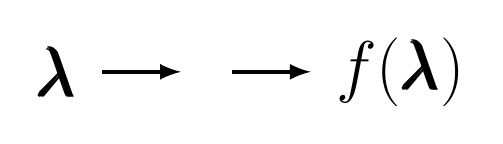
\begin{tikzpicture}
\tikzstyle{every node}=[draw,fill=white,minimum width=0cm,thin]
\tikzstyle{every path}=[-latex,ultra thick]
\node (A) [draw=white]{{\Huge{$\conf$}}};
\node (B) [right=14mm of A,draw=white] {\myblackbox{}};
\node (C) [right=14mm of B,draw=white] {{\Huge{$f(\conf)$}}};
%\node (D) [below=7mm of B, align=center, fill=black!10] {\large{Bayesian}\\\large{optimization}};

\draw ($(A.east)+(0.2,0.0)$) -- ($(B.west)+(-0.2,0.0)$);
\draw ($(B.east)+(0.2,0.0)$) -- ($(C.west)+(-0.2,0.0)$);
%\draw ($(C.south)+(0.0,-0.2)$) -| ++(0.0,0.0) |- ($(D.east)+(0.2,0.0)$);
%\draw ($(D.west)+(-0.2,0.0)$) |- ++(0.0,0.0) -| ($(A.south)+(0.0,-0.2)$);
\end{tikzpicture}
}
    	\end{center}
    	\myit{
    		\item Only mode of interaction with $f$: querying $f$'s value at a given $\conf$ 
            \item Function $f$ may not be available in closed form, not differentiable, noisy, etc. 
    	}   
\medskip
\pause

        \item Today, we'll discuss a \alert{Bayesian} approach for solving such blackbox optimization problems
\medskip
\pause
        \item Blackbox optimization can be used for hyperparameter optimization (HPO)
        \myit{
            \item Define \alert{$f(\conf) := \mathcal{L}( \mathcal{A}_{\conf}, \mathcal{D}_{train}, \mathcal{D}_{valid} )$}
    \pause
            \item Note: for formulations of HPO that go beyond blackbox optimization, see next lecture
        }
    }
}

%----------------------------------------------------------------------
%\begin{frame}[c]{Optimization problem example}

%We know that:
%\begin{itemize}
%    \item The function $\cost$ is Lipschitz continuous and differentiable.
%    \pause
%    \item The minimizer of $\cost$ is in the interval [0,1].
%    \pause
%    \item We have observed 3 evaluations of $\cost$.
%\end{itemize}

%\end{frame}
%----------------------------------------------------------------------
%\begin{frame}[c]{Problem description}
%\framesubtitle{We have 4 function evaluations}
%\begin{figure}
%    \centering
%    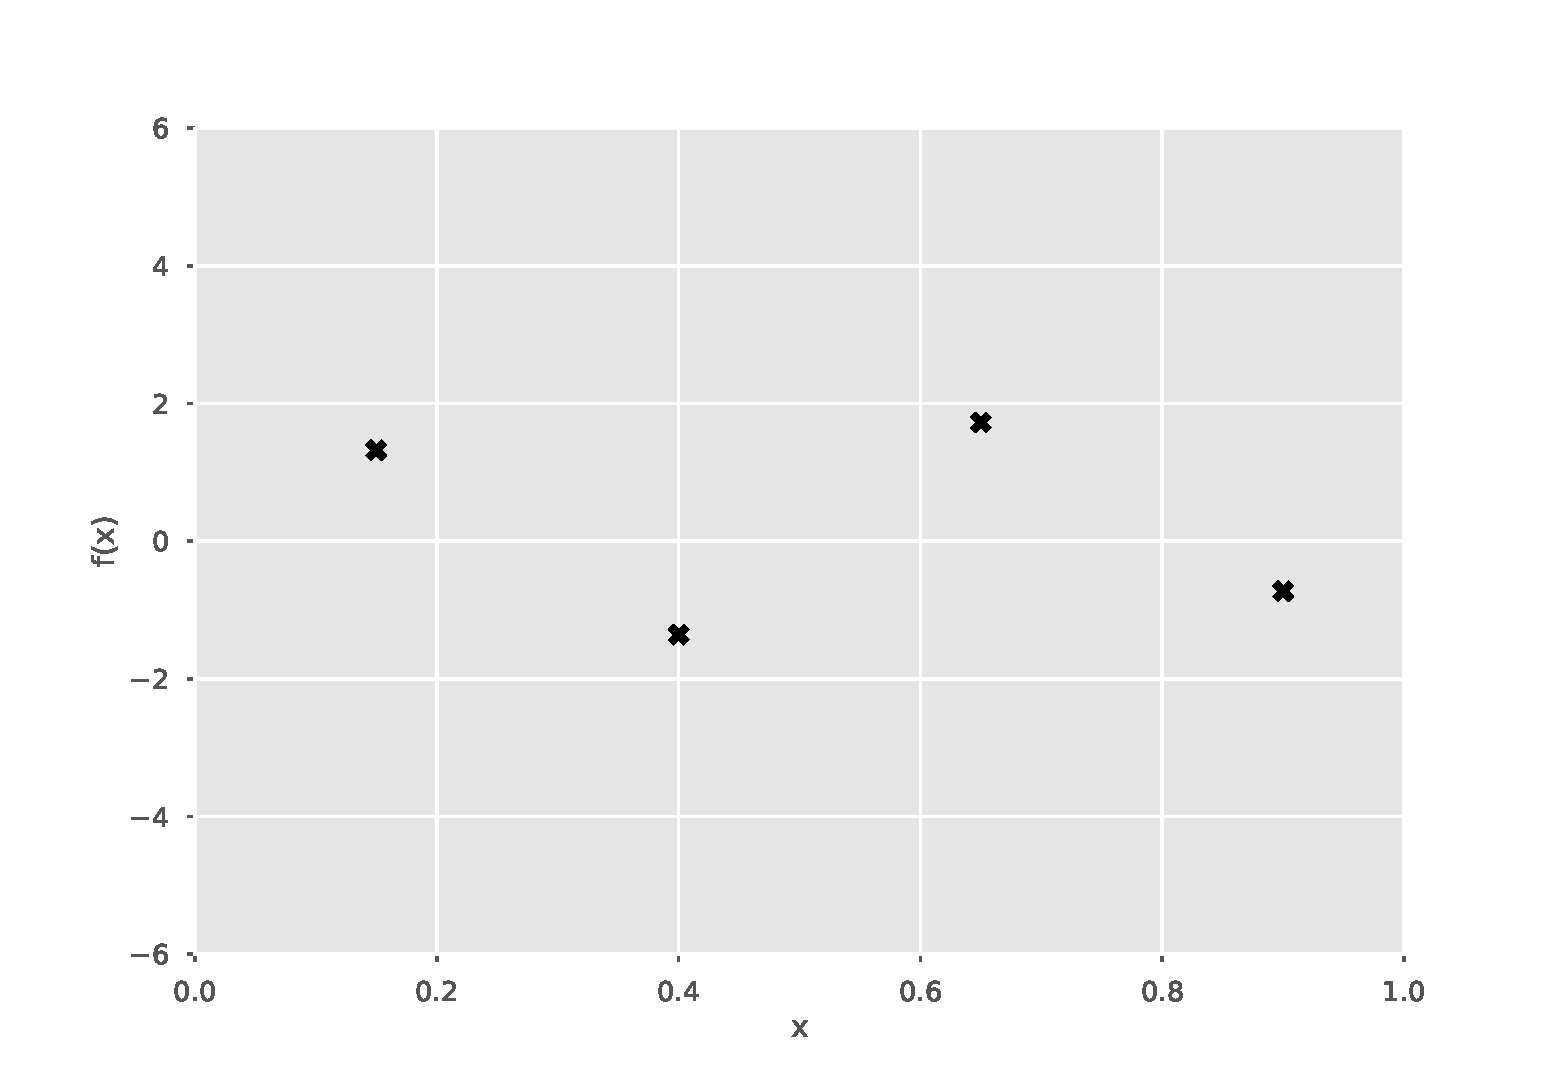
\includegraphics[width=0.8\textwidth, %height=0.38\textwidth]{images/intro_images/plot_datapoints.p%df}
%    \label{fig:my_label}
%\end{figure}
%\begin{center}
%  Where is the minimum of function $f$?  
%\end{center}
%\source{Plots are based on Javier Gonz\'alez's BO lecture %(bo\_intro.py)}



%\end{frame}

%-----------------------------------------------------------------------
%----------------------------------------------------------------------
%\begin{frame}[c]{Problem description}
%\framesubtitle{One possible curve}
%\begin{figure}
%    \centering
%    \includegraphics[width=0.7\textwidth, %height=0.4\textwidth]{images/intro_images/plot_posterior_1_s%ample.pdf}
%    \label{fig:my_label}
%\end{figure}
%\source{Plots are based on Javier Gonz\'alez's BO lecture %(bo\_intro.py)}



%\end{frame}

%-----------------------------------------------------------------------
%----------------------------------------------------------------------
%\begin{frame}[c]{Problem description}
%\framesubtitle{Three possible curves}
%\begin{figure}
%    \centering
%    \includegraphics[width=0.7\textwidth, %height=0.4\textwidth]{images/intro_images/plot_posterior_3_s%ample.pdf}
%    \label{fig:my_label}
%\end{figure}
%\source{Plots are based on Javier Gonz\'alez's BO lecture %(bo\_intro.py)}



%\end{frame}

%-----------------------------------------------------------------------
%----------------------------------------------------------------------
%\begin{frame}[c]{Problem description}
%\framesubtitle{Ten possible curves}
%\begin{figure}
%    \centering
%    \includegraphics[width=0.7\textwidth, %height=0.4\textwidth]{images/intro_images/plot_posterior_10_%sample.pdf}
%    \label{fig:my_label}
%\end{figure}
%\source{Plots are based on Javier Gonz\'alez's BO lecture %(bo\_intro.py)}



%\end{frame}

%-----------------------------------------------------------------------
%----------------------------------------------------------------------
%\begin{frame}[c]{Problem description}
%\framesubtitle{One hundred possible curves}
%\begin{figure}
%    \centering
%    \includegraphics[width=0.7\textwidth, %height=0.4\textwidth]{images/intro_images/plot_posterior_100%_sample.pdf}
%    \label{fig:my_label}
%\end{figure}
%\source{Plots are based on Javier Gonz\'alez's BO lecture %(bo\_intro.py)}



%\end{frame}

%-----------------------------------------------------------------------%----------------------------------------------------------------------
%\begin{frame}[c]{Problem description}
%\framesubtitle{One thousand possible curves}
%\begin{figure}
%    \centering
%    \includegraphics[width=0.7\textwidth, %height=0.4\textwidth]{images/intro_images/plot_posterior_100%0_sample.pdf}
%    \label{fig:my_label}
%\end{figure}
%\source{Plots are based on Javier Gonz\'alez's BO lecture (bo\_intro.py)}



%\end{frame}

%-----------------------------------------------------------------------
%----------------------------------------------------------------------
%\begin{frame}[c]{Problem description}
%\framesubtitle{Infinitely many curves}
%\begin{figure}
%    \centering
%    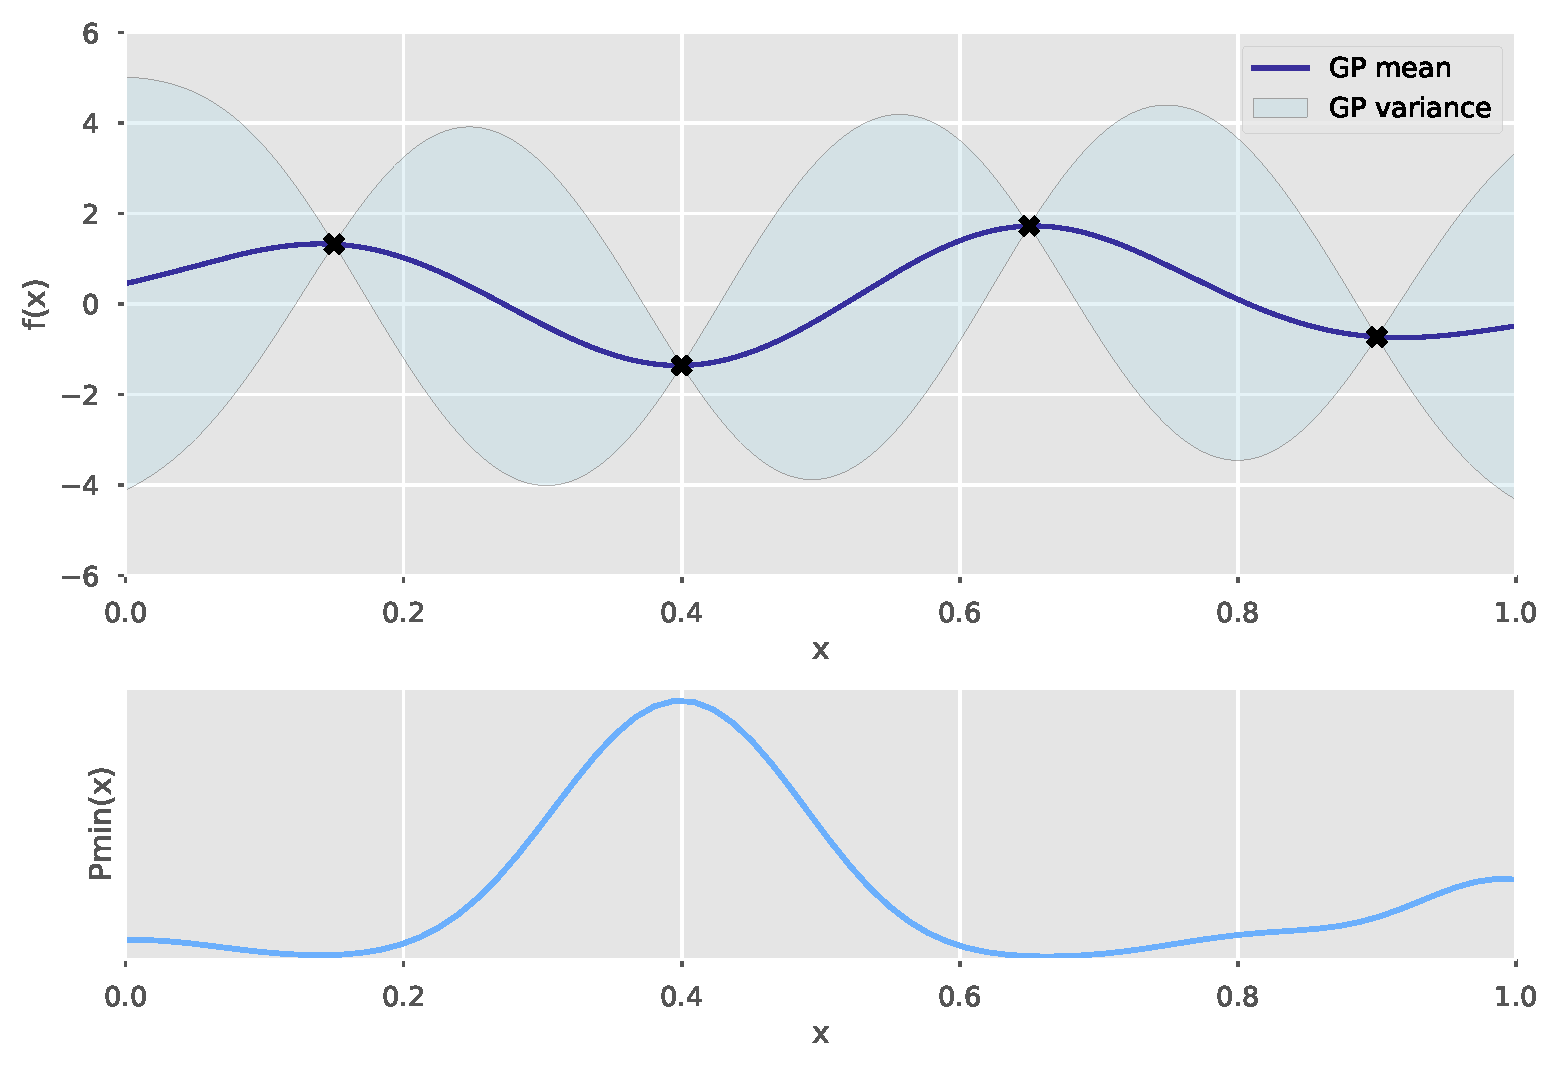
\includegraphics[width=0.7\textwidth, %height=0.4\textwidth]{images/intro_images/plot_posterior.pdf%}
%    \label{fig:my_label}
%\end{figure}
%\source{Plots are based on Javier Gonz\'alez's BO lecture (bo\_intro.py)}


%\end{frame}
%----------------------------------------------------------------------
\myframetop{Bayesian Optimization of a blackbox function in a nutshell}{

\bigskip
\bigskip
\bigskip

    \onslide<1->
    \begin{figure}
        \vspace{-1em}
        \centering
        \only<1>{
            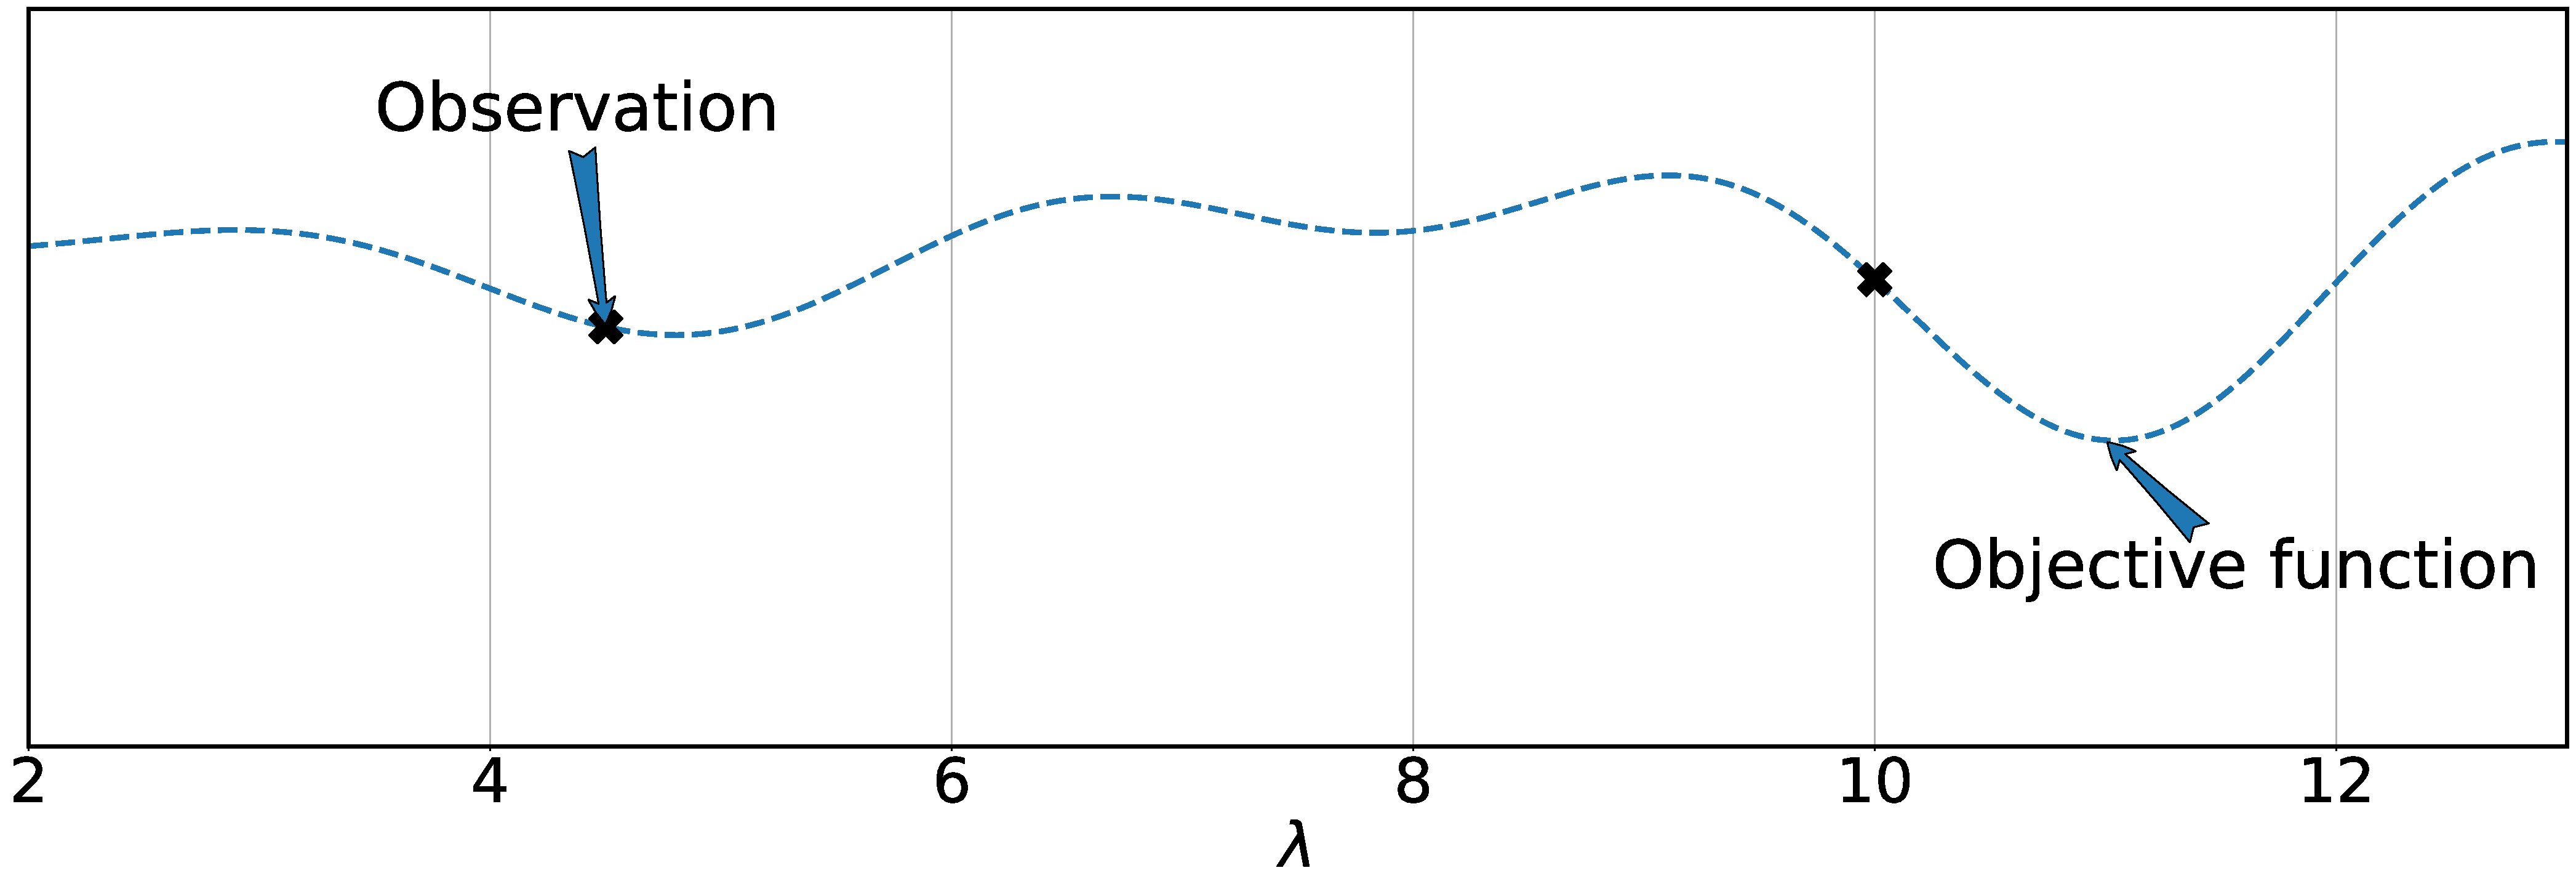
\includegraphics[width=0.95\textwidth]{images/intro_images/IntroPlots_Obs.pdf}
        }\only<2>{
            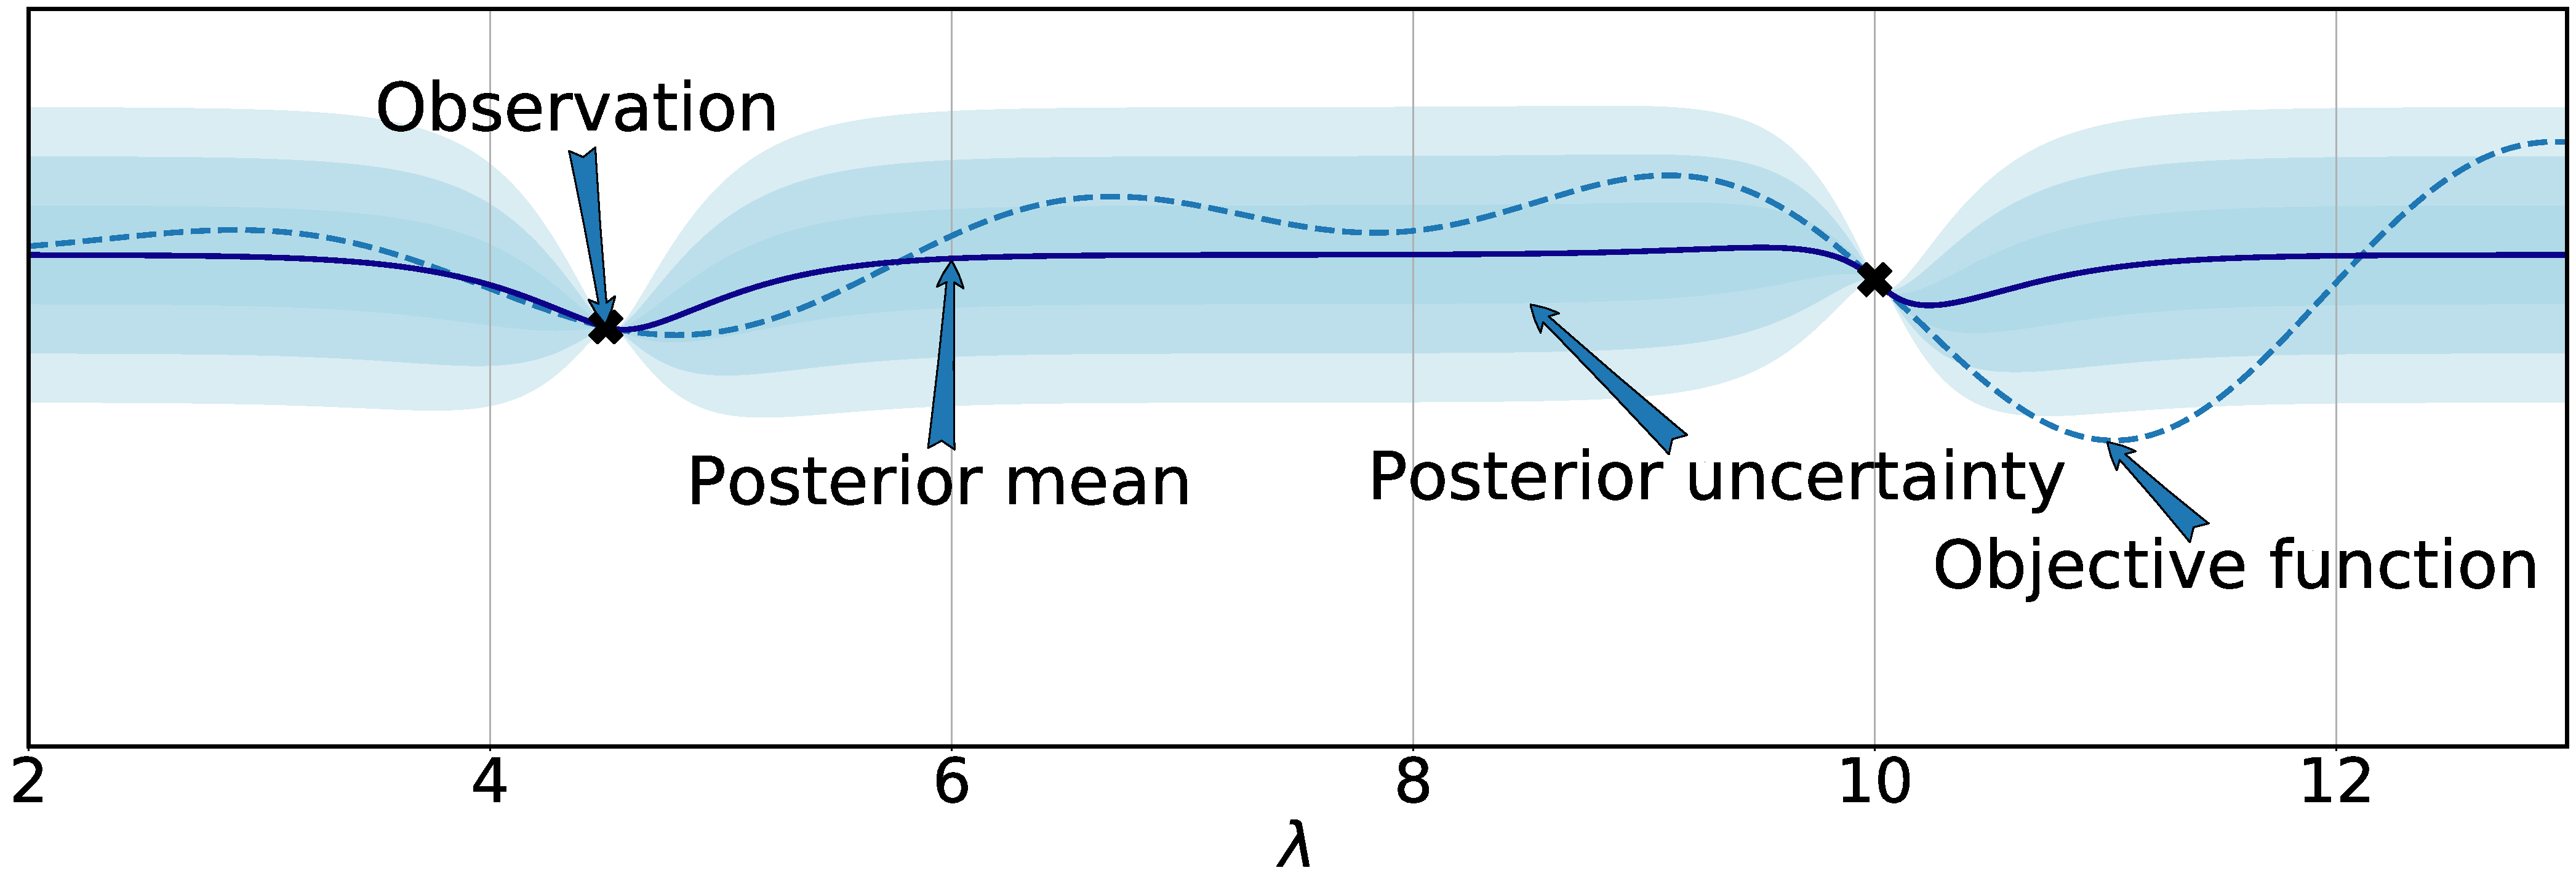
\includegraphics[width=0.95\textwidth]{images/intro_images/IntroPlots_GP.pdf}
        }\only<3>{
            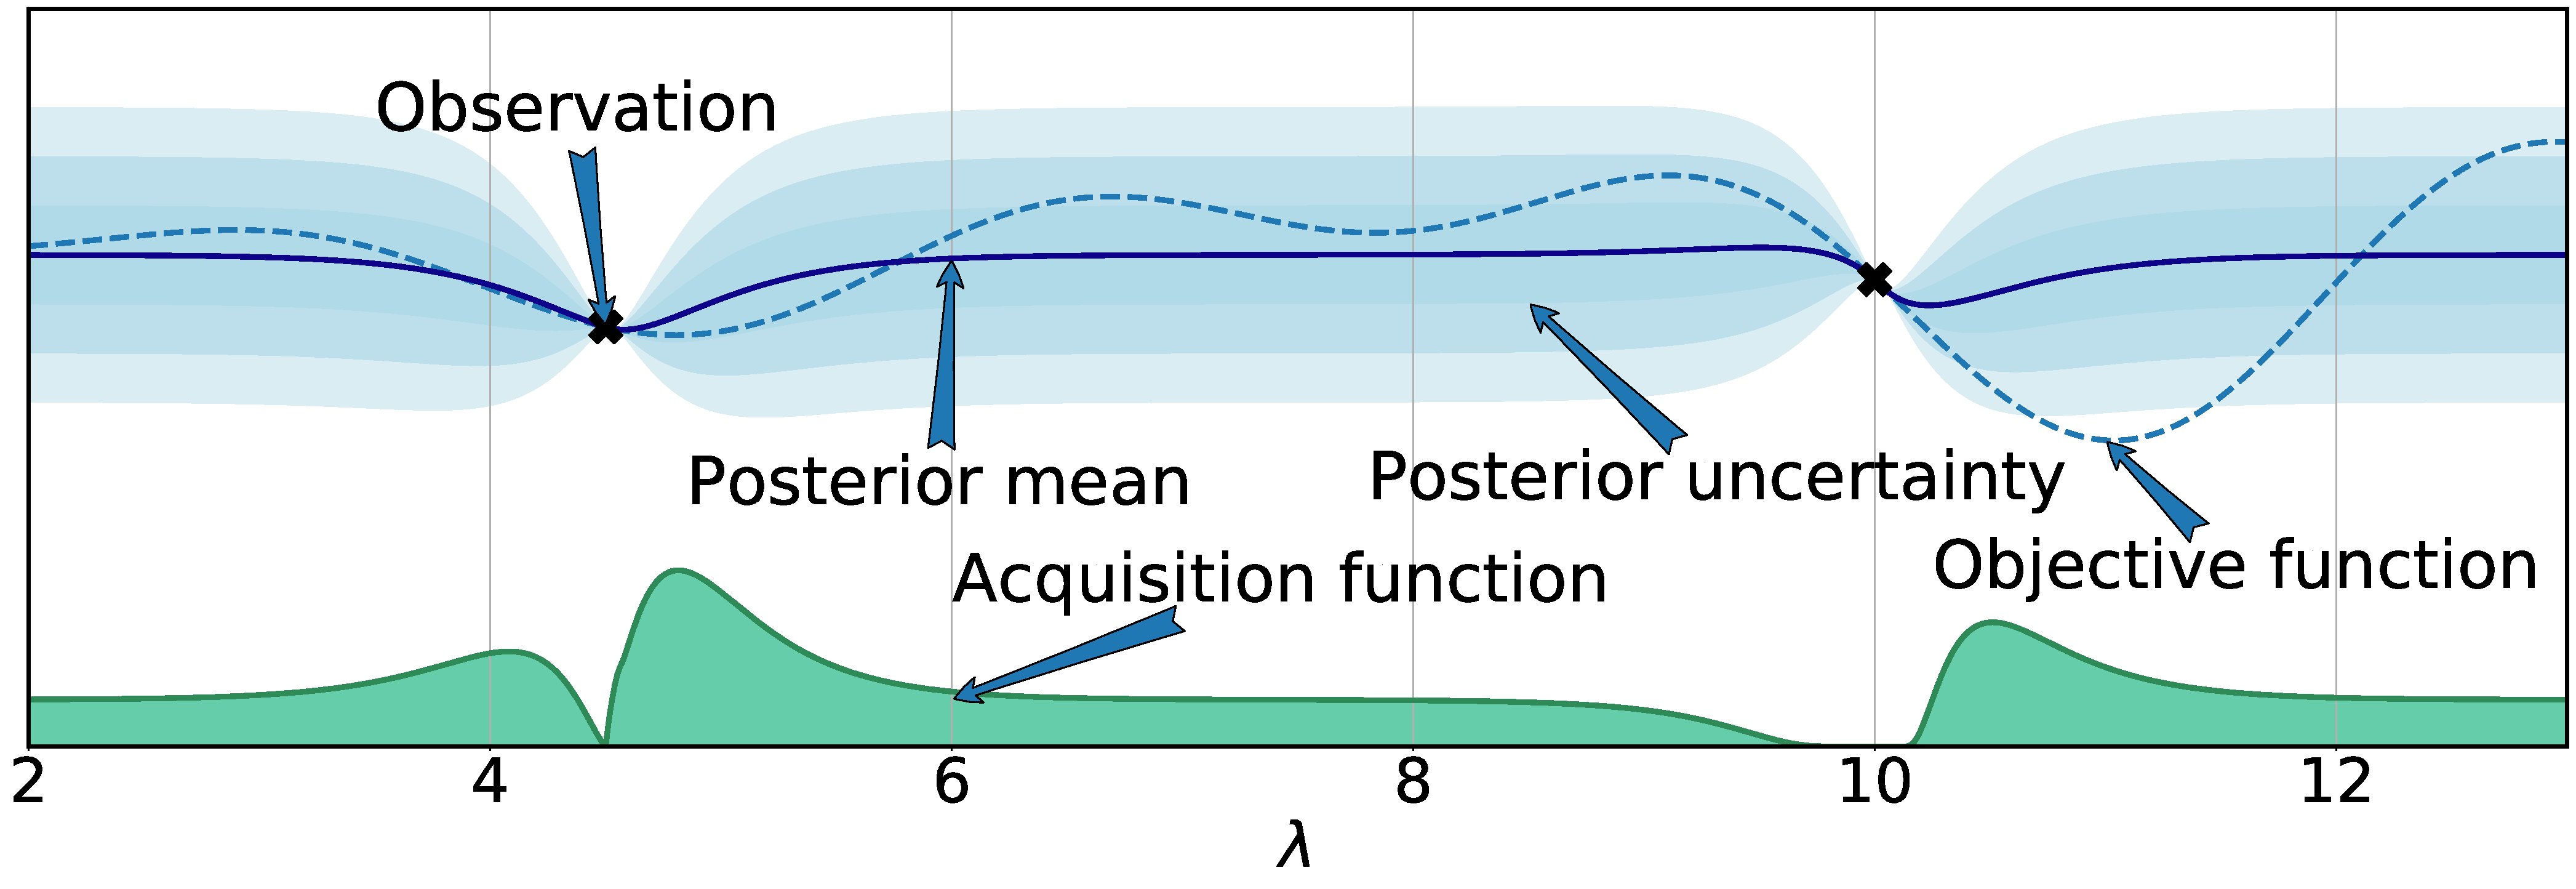
\includegraphics[width=0.95\textwidth]{images/intro_images/IntroPlots_Acqui.pdf}
        }\only<4->{
            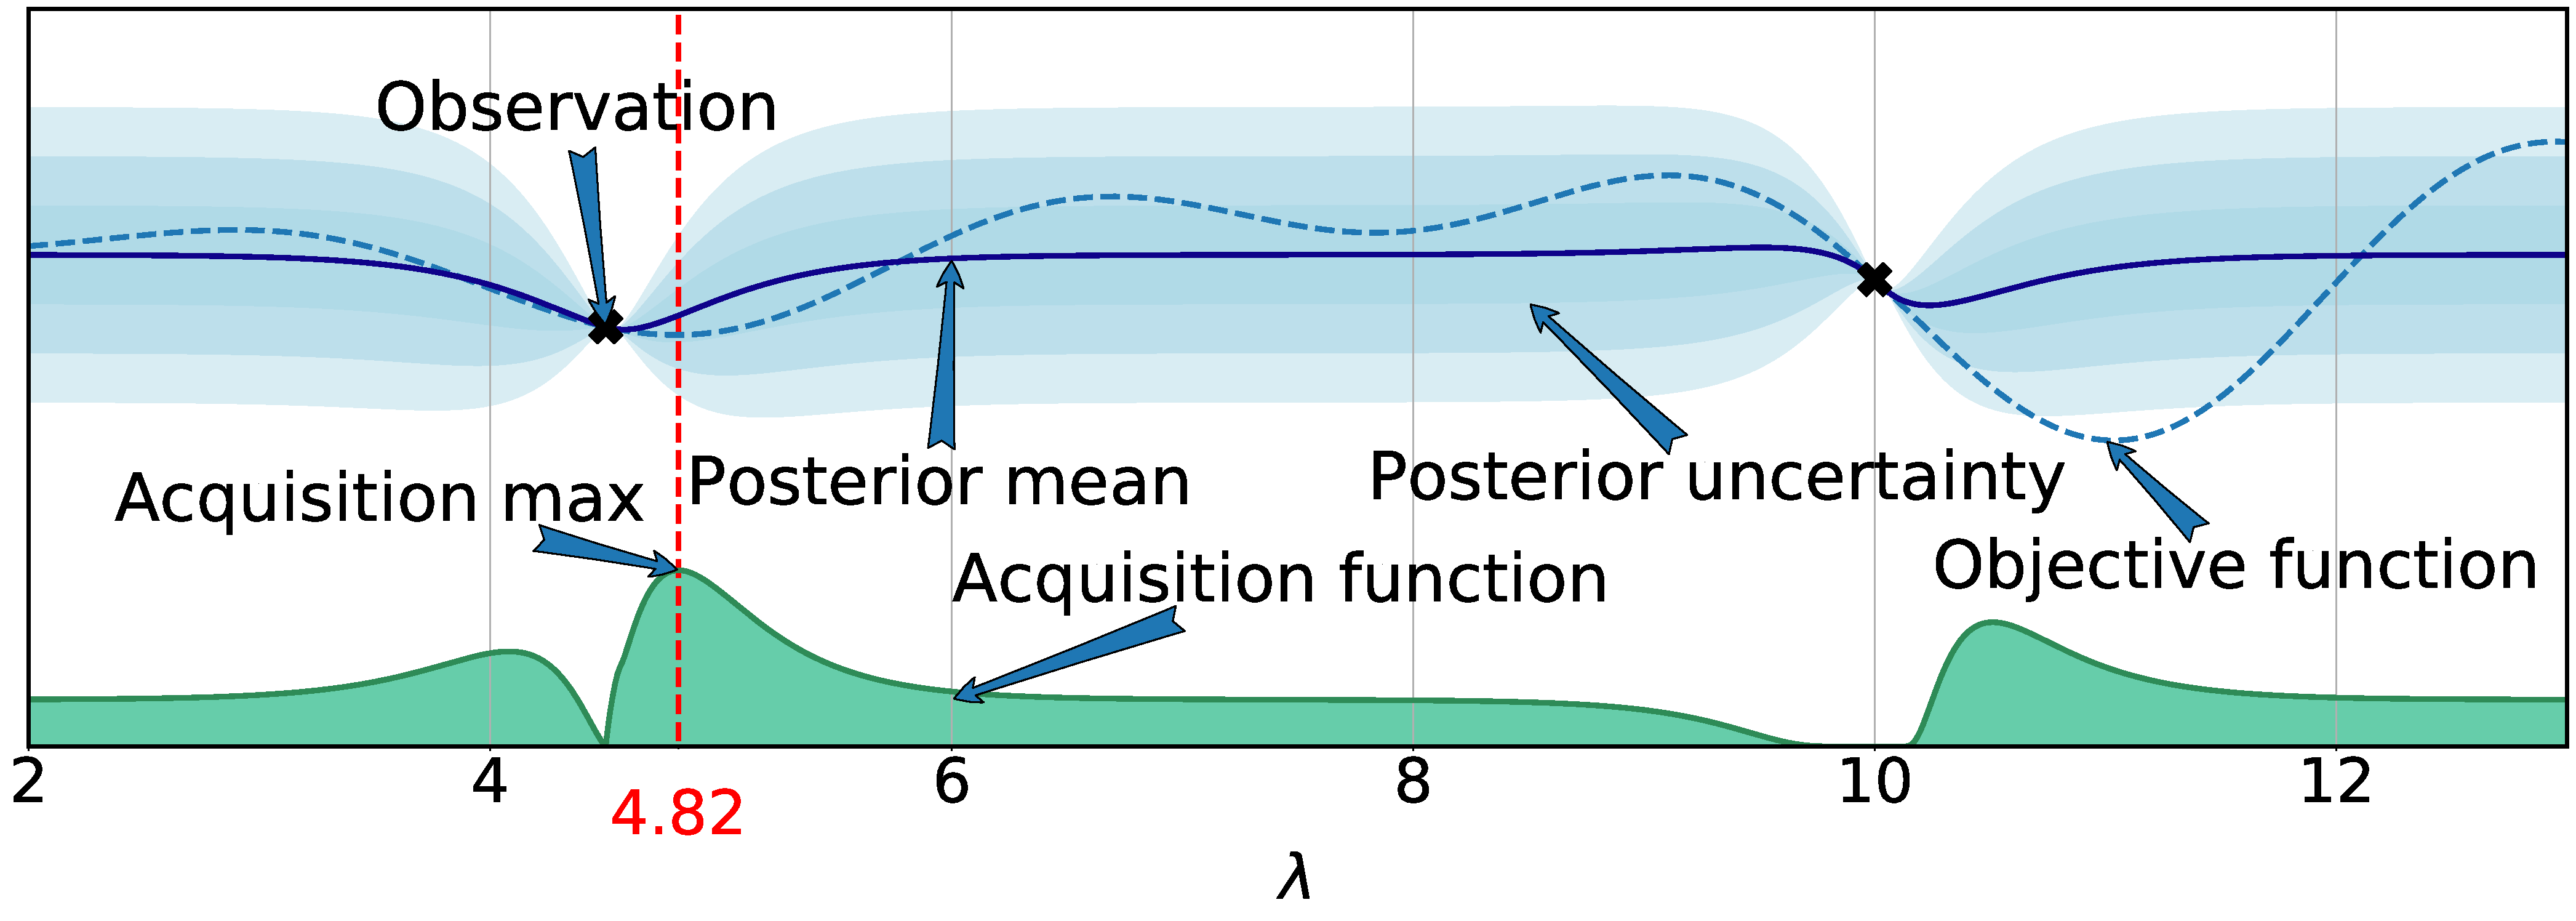
\includegraphics[width=0.95\textwidth]{images/intro_images/IntroPlots_Complete.pdf}
        }
    \end{figure}
    
% \vspace*{-0.5cm}\notefh{Can you please increase the plotted values of the acquisition function, so that it is more clearly visible? Also on the next slide. You could, e.g., normalize it to have a certain maximum (a bit larger than that of the third plot on the next slide). Also, on the next slide, can you please plot the new observation red, not green?}
}

%----------------------------------------------------------------------
\begin{frame}[c]{Bayesian Optimization of a blackbox function in a nutshell}

\begin{columns}[T]
\column{0.45\textwidth}
General approach
\begin{itemize}
    \item Fit a \alert{probabilistic model} to the collected function samples $\langle{}\conf, \cost(\conf)\rangle{}$
    \item Use the model to guide optimization, trading off \alert{exploration \vs{} exploitation}
%    \item Acquisition function for exploration-exploitation tradeoff
%    \item Optimize on acquisition function\\ to get next $x$ $\conf$ ($x$)
\end{itemize}

\bigskip

\onslide<4->{
    \alert{Popular approach in the statistics literature} since
    \href{http://link.springer.com/chapter/10.1007\%2F3-540-07165-2_55}{\footnotesize\color{black!70} Mockus et al. [1978]}
    \begin{itemize}
        \item Efficient in \#function evaluations
        \item Works when objective is \alert{nonconvex, noisy, has unknown derivatives, etc.}
        \item Recent \alert{convergence} results\\ \lit{\href{https://arxiv.org/abs/0912.3995}{Srinivas et al. 2009}; \href{http://www.jmlr.org/papers/v12/bull11a.html}{Bull et al. 2011}; \href{https://www.cs.ubc.ca/~nando/papers/BayesBandits.pdf}{de Freitas et al. 2012}; \href{http://papers.nips.cc/paper/5715-bayesian-optimization-with-exponential-convergence}{Kawaguchi et al. 2015}}
    %    \item Popular \alert{Bayesian optimization workshop} at NIPS (the premiere machine learning conference)
    \end{itemize}
}

\column{0.55\textwidth}
\onslide<1->
\begin{figure}
    \vspace{-1em}
    \centering
    \onslide<1->{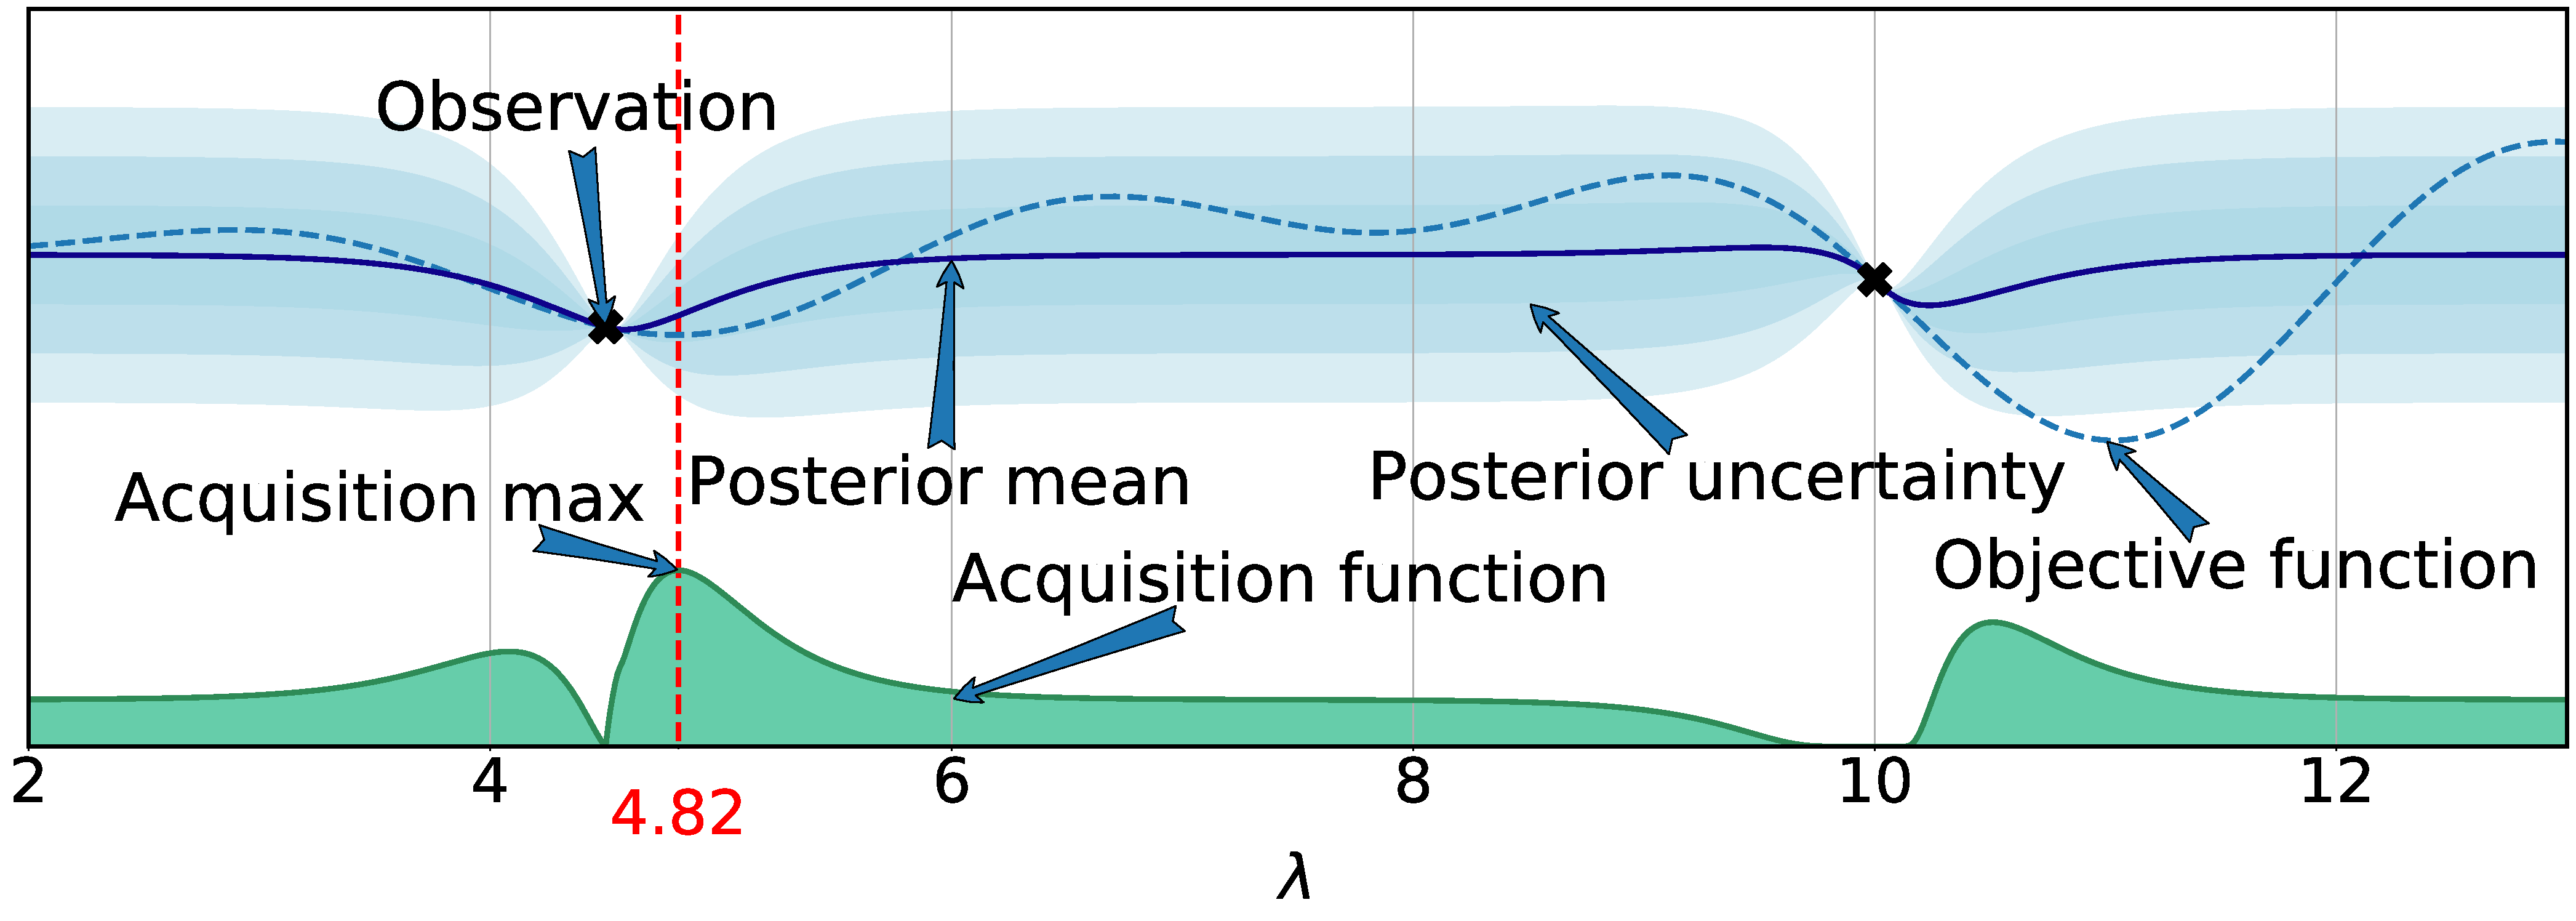
\includegraphics[width=0.8\textwidth]{images/intro_images/IntroPlots_Iter2.pdf}}
    \onslide<2->{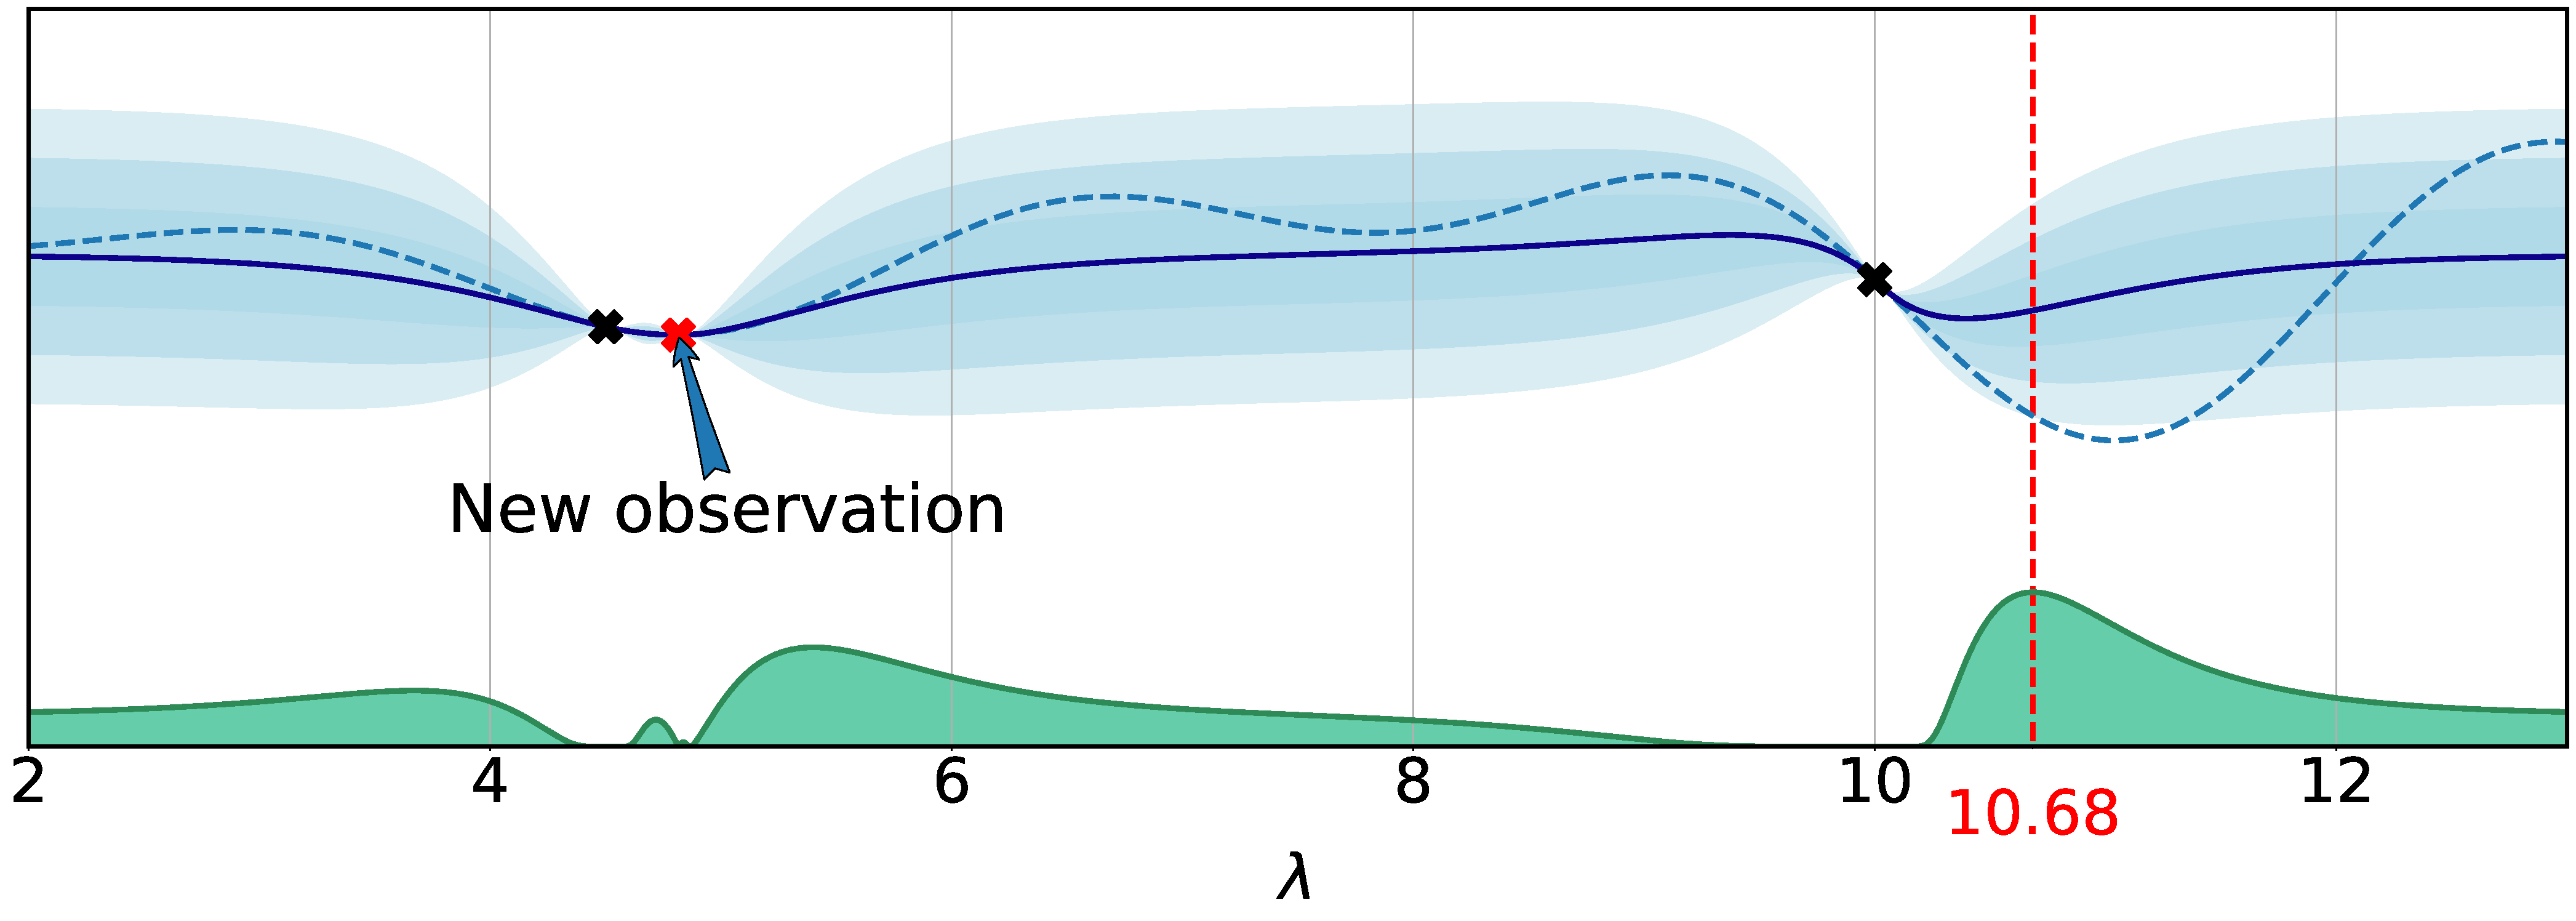
\includegraphics[width=0.8\textwidth]{images/intro_images/IntroPlots_Iter3.pdf}}
    \onslide<3->{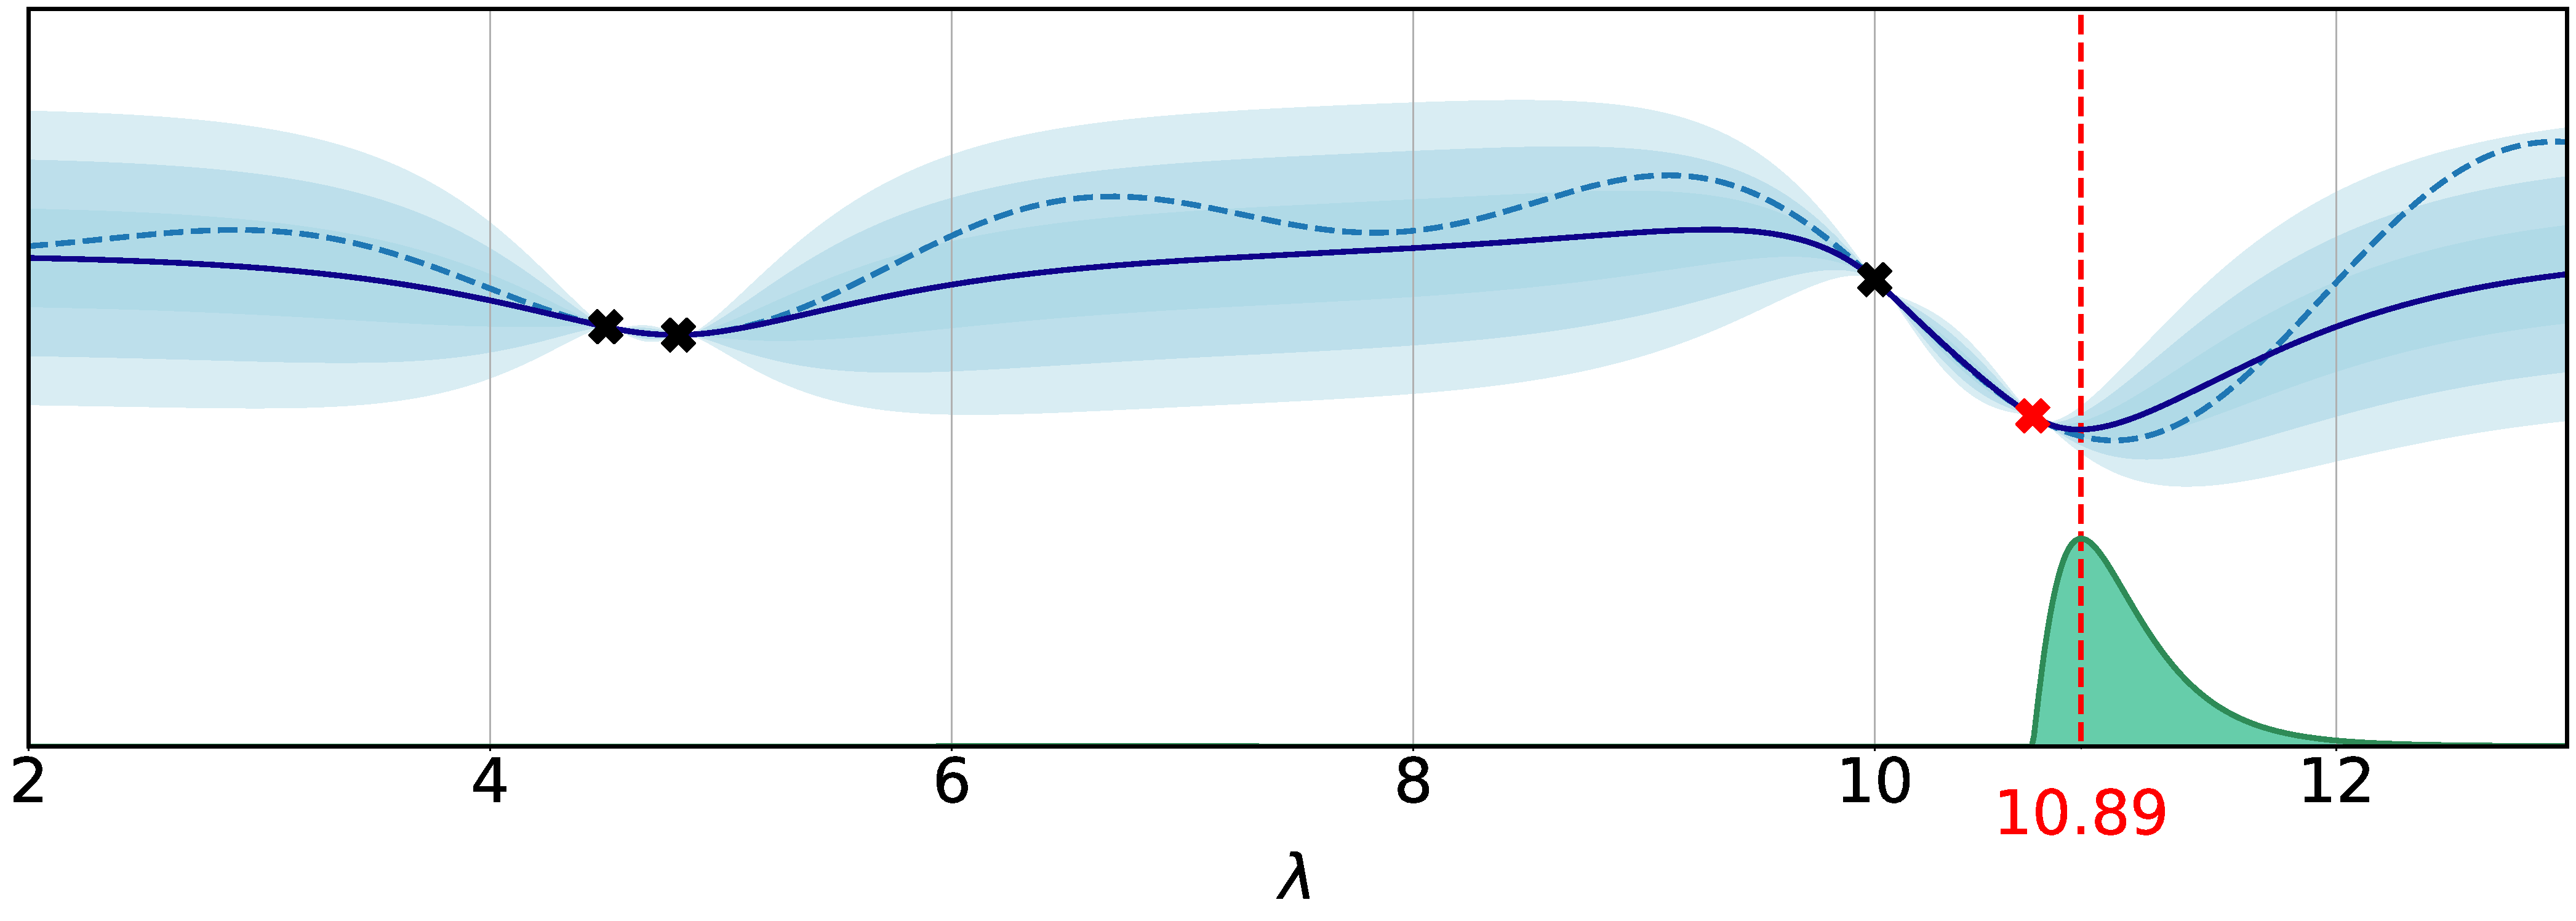
\includegraphics[width=0.8\textwidth]{images/intro_images/IntroPlots_Iter4.pdf}}
    %\only<4>{\includegraphics[width=\textwidth]{images/intro_images/plot_2.pdf}}
    %\only<5>{\includegraphics[width=\textwidth]{images/intro_images/plot_3.pdf}}
    %\only<6>{\includegraphics[width=\textwidth]{images/intro_images/plot_4.pdf}}
    %\only<7>{\includegraphics[width=\textwidth]{images/intro_images/plot_5.pdf}}
    %\only<8>{\includegraphics[width=\textwidth]{images/intro_images/plot_6.pdf}}
    %\only<9->{\includegraphics[width=\textwidth]{images/intro_images/plot_7.pdf}}
\end{figure}
\end{columns}

\end{frame}
%-----------------------------------------------------------------------
%\myframe{Bayesian Optimization in a Nutshell}{
%  
%\vspace*{-0.5cm}
%\begin{columns}[T]
%
%\column{0.6\textwidth}
%
%\myblock{General approach}{
%	\myit{
%	  \item Fit a probabilistic model to the collected function samples
%	  $\langle{}\conf, \cost(\conf)\rangle{}$
%	  \item Use the model to guide optimization, trading off
%	  exploration \vs{} exploitation
%	%  \item Acquisition function for exploration-exploitation tradeoff
%	%  \item Optimize on acquisition function\\ to get next $x$
%	  %$\conf$ ($x$)
%	}
%}
%
%\smallskip
%\onslide<5->{
%	\myblock{Popular approach in the statistics literature since \litw{\href{http://link.springer.com/chapter/10.1007\%2F3-540-07165-2_55}{Mockus,
%	1978}}}{ \myit{
%		  	\item Efficient in \# function evaluations 
%		  	\item Works when objective is nonconvex, noisy, has unknown derivatives, etc
%			\pause
%			\item Recent convergence results\\ \lit{Srinivas et al, 2010; Bull 2011;
%			de Freitas et al, 2012; Kawaguchi et al, 2015}
%			%TODO: sorry, I don't know these papers
%		%	\item Popular \alert{Bayesian optimization workshop} at NIPS (the premiere machine learning conference)
%		}
%	}
%}
%%\begin{enumerate}
%%  \item Fit an empirical performance model (EPM) 
%%  \item Acquisition function for exploration-exploitation tradeoff
%%  \item Optimize on acquisition function\\ to get next $\conf$ ($x$)
%%\end{enumerate}
%
%\column{0.4\textwidth}
%\vspace*{0.5cm}
%\onslide<2->{
%	%\includegraphics[width=1\textwidth]{../images/bo.png}
%	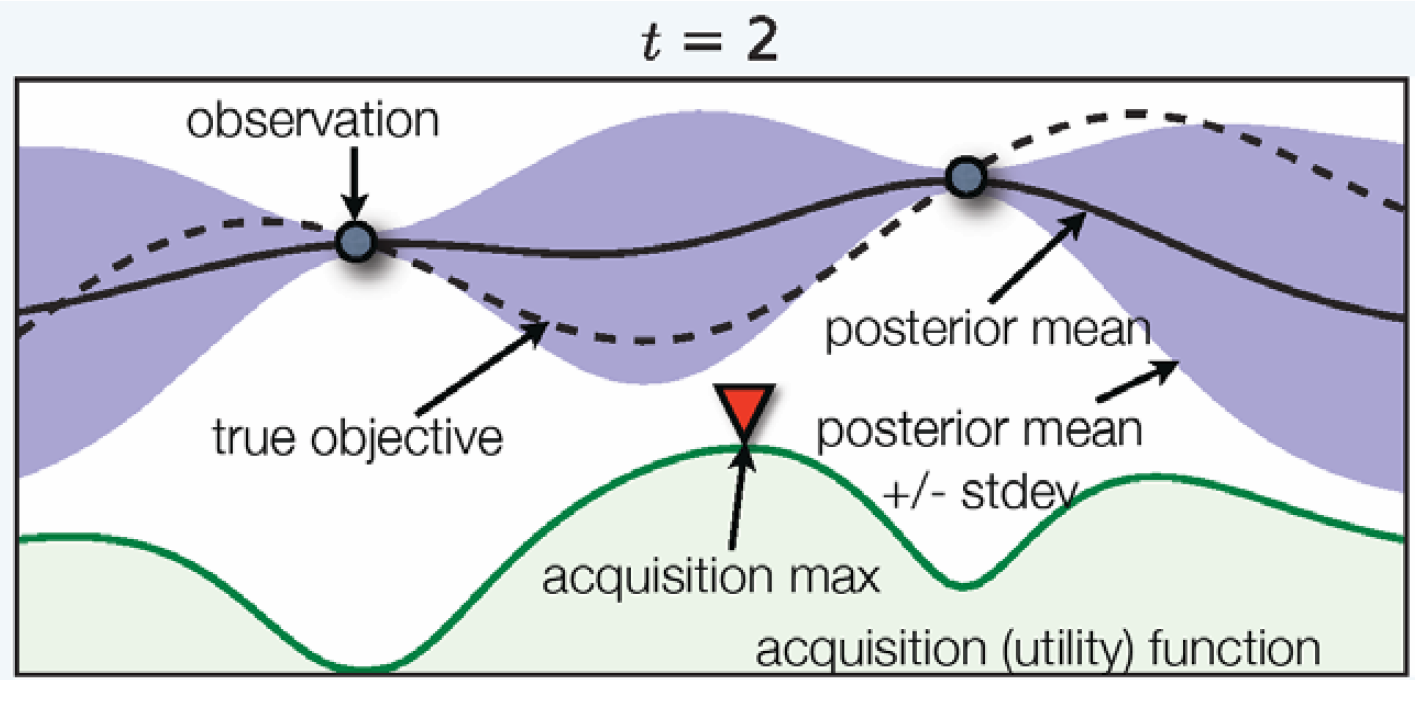
\includegraphics[width=0.9\textwidth]{plots_and_scripts/plots/bo_pic1.png}\\
%	\pause
%	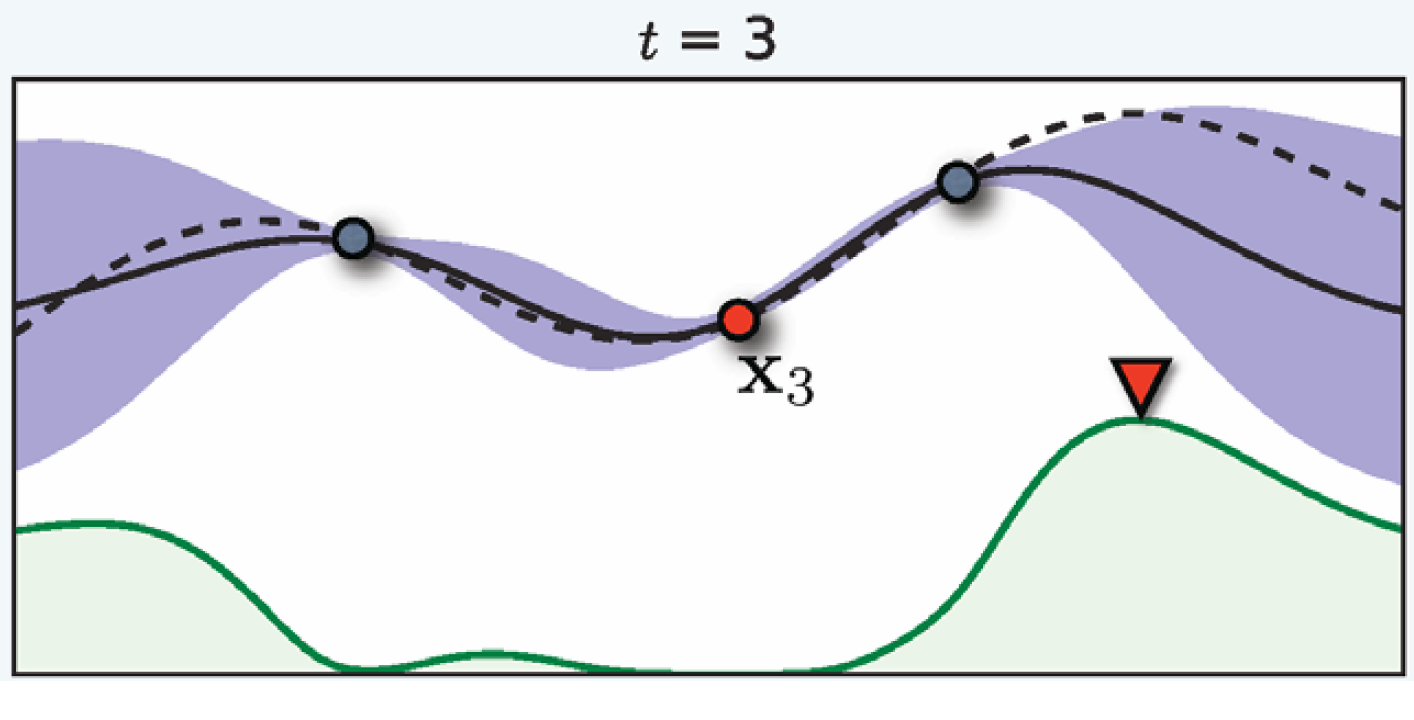
\includegraphics[width=0.9\textwidth]{plots_and_scripts/plots//bo_pic2.png}\\
%	\pause
%	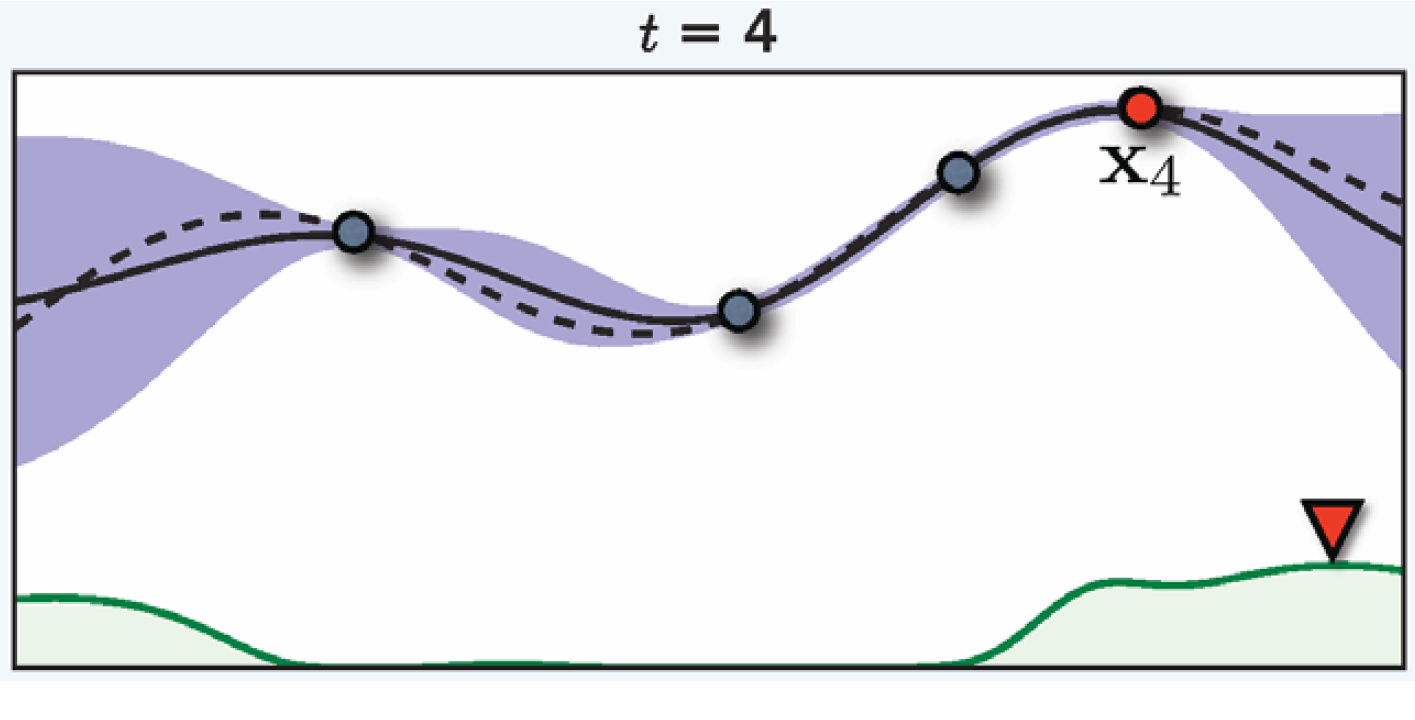
\includegraphics[width=0.9\textwidth]{plots_and_scripts/plots//bo_pic3.png}\\
%	\footnotesize{Image source: \lit{\href{https://arxiv.org/abs/1012.2599}{Brochu et al, 2010}}}
%}
%\end{columns}
%}
%----------------------------------------------------------------------
%5\begin{frame}[c]{Bayesian Optimization: Visualization of Many Steps}
%\begin{figure}
%    \centering
%    \only<1>{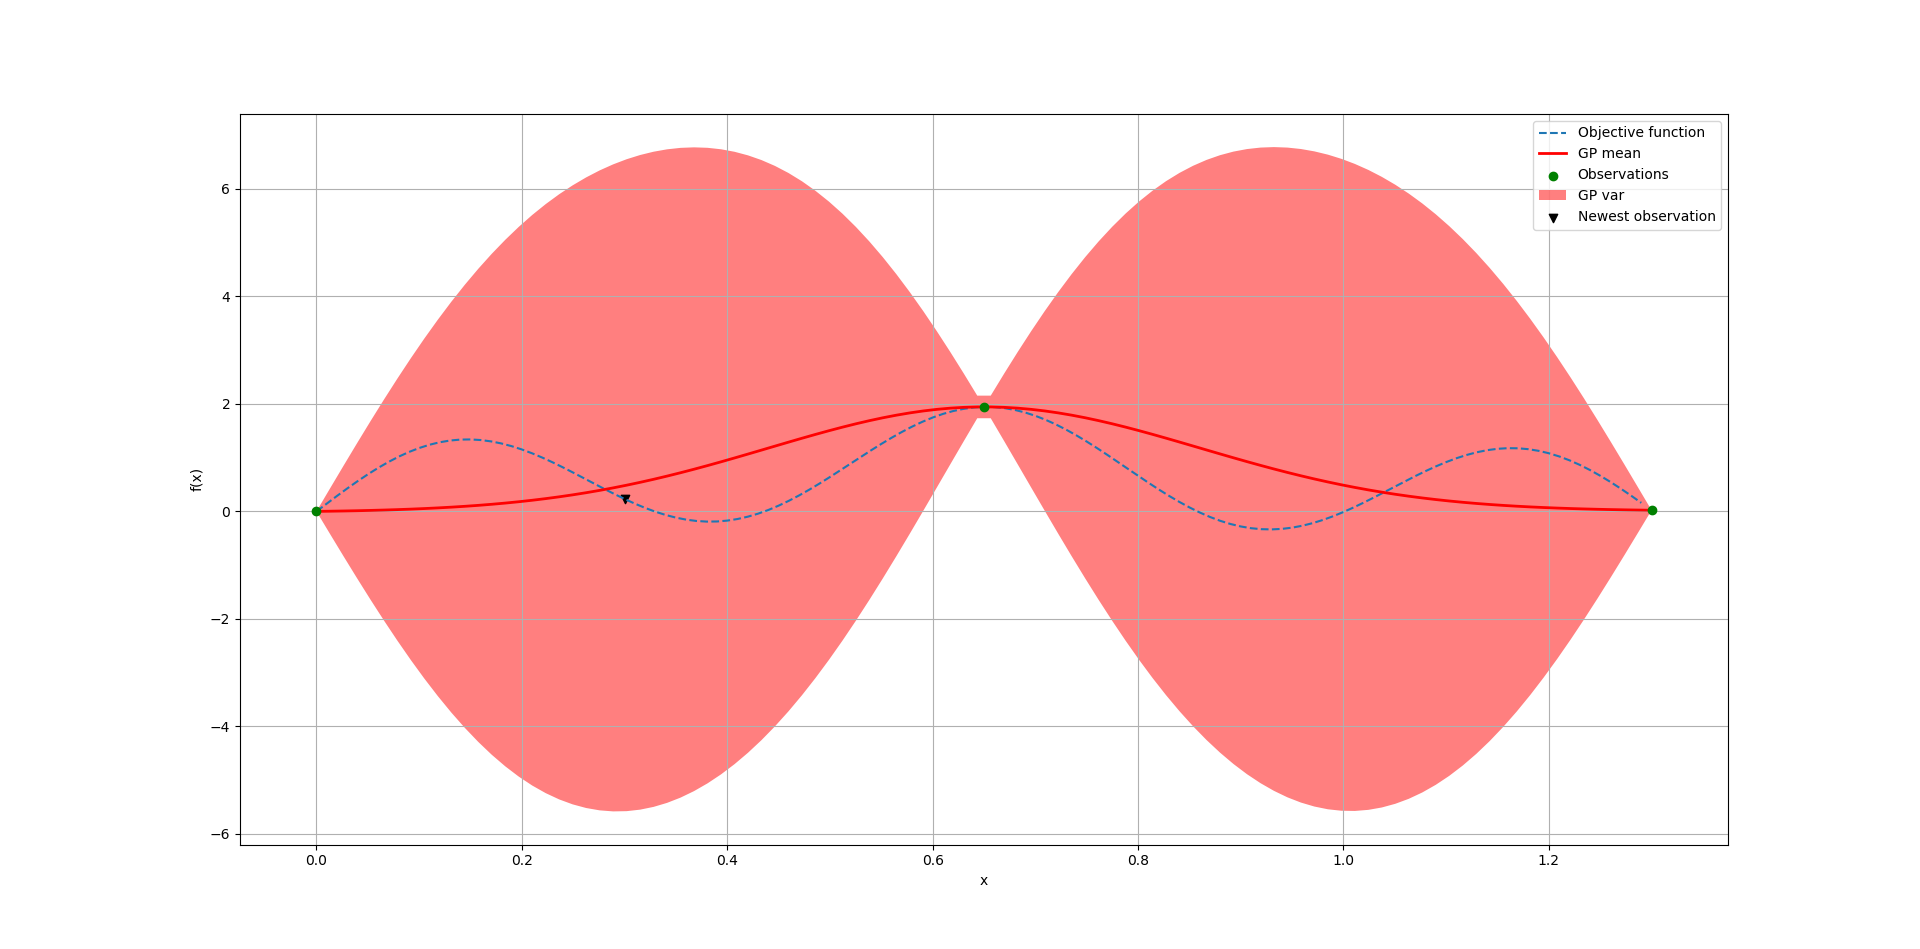
\includegraphics[width=\linewidth]{images/intro_images/BOLoop_1.png}}
%    \only<2>{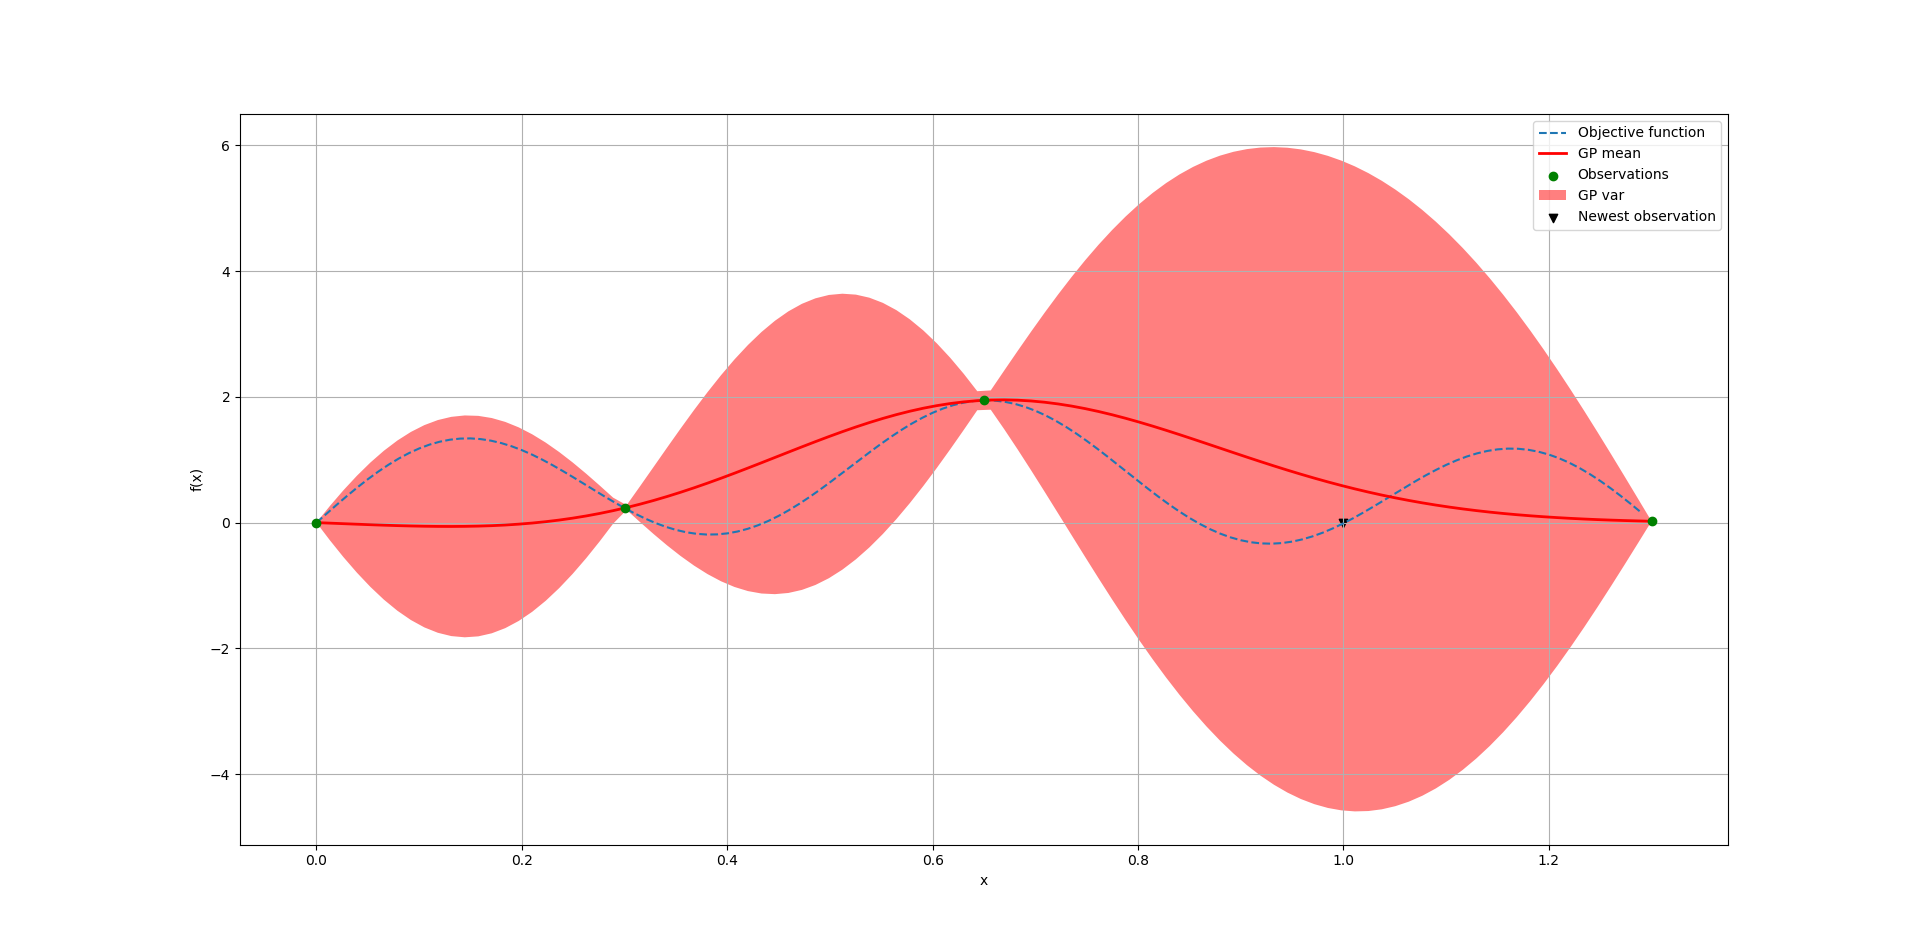
\includegraphics[width=\linewidth]{images/intro_images/BOLoop_2.png}}
%    \only<3>{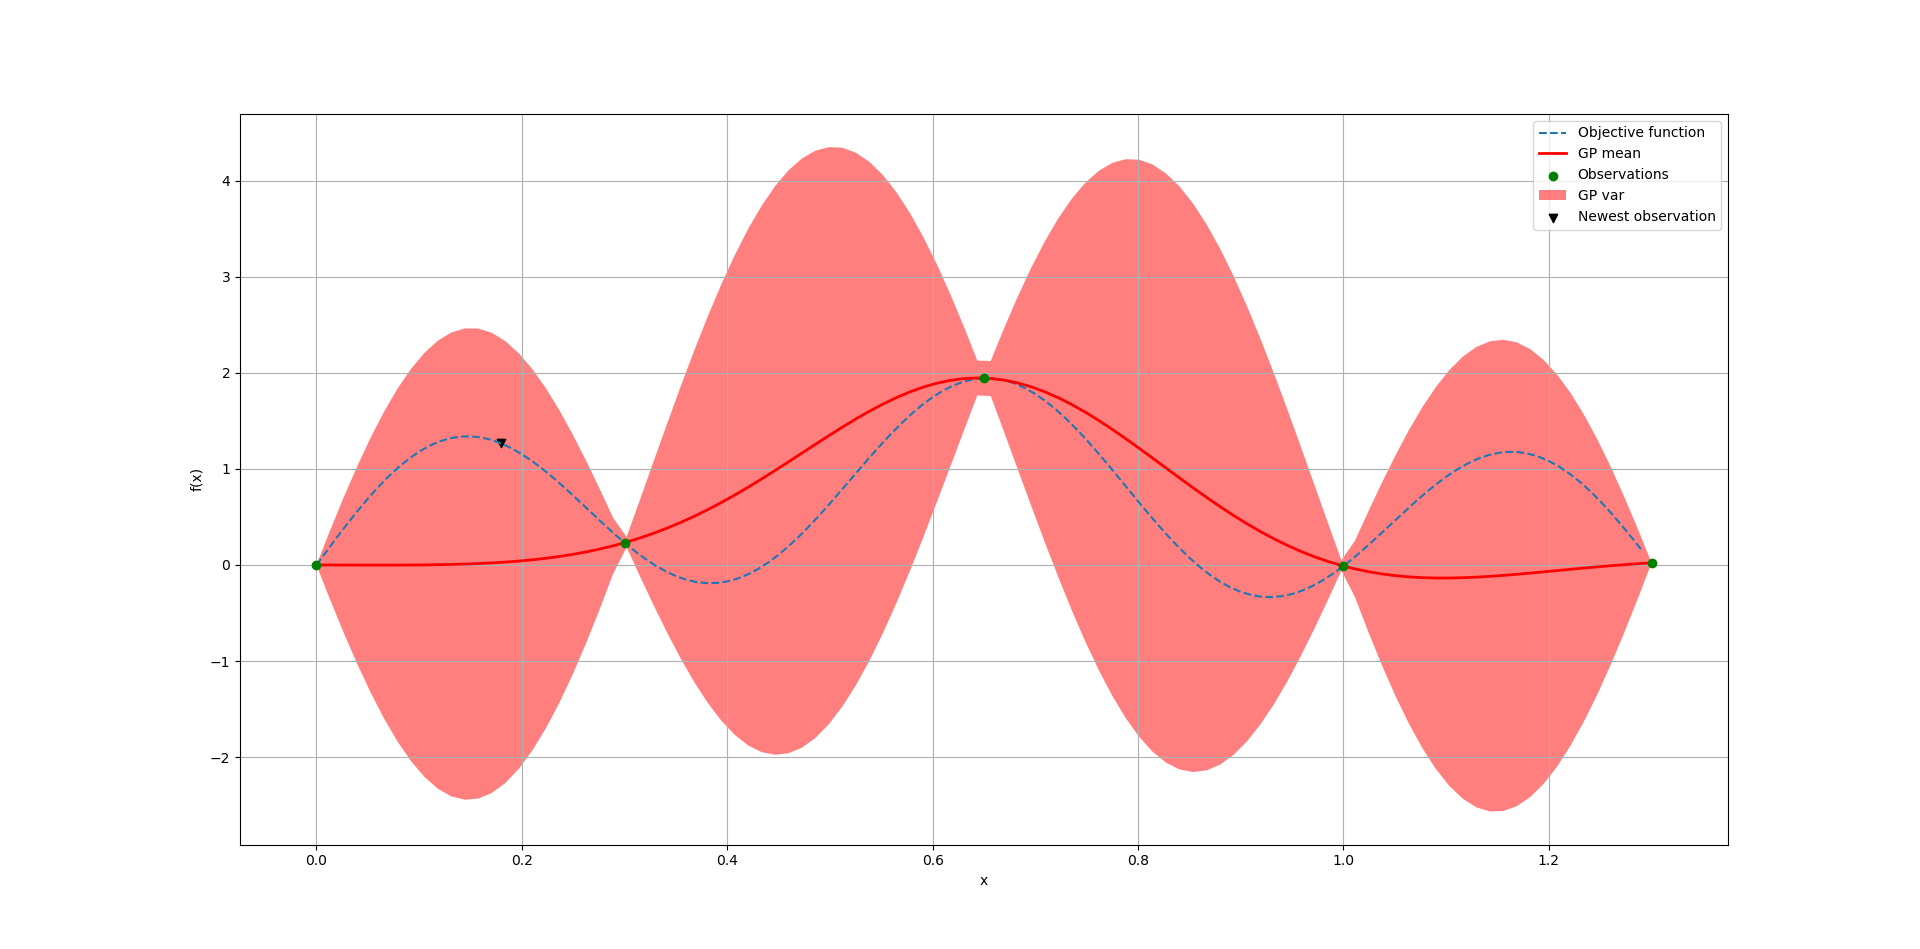
\includegraphics[width=\linewidth]{images/intro_images/BOLoop_3.png}}
%    \only<4>{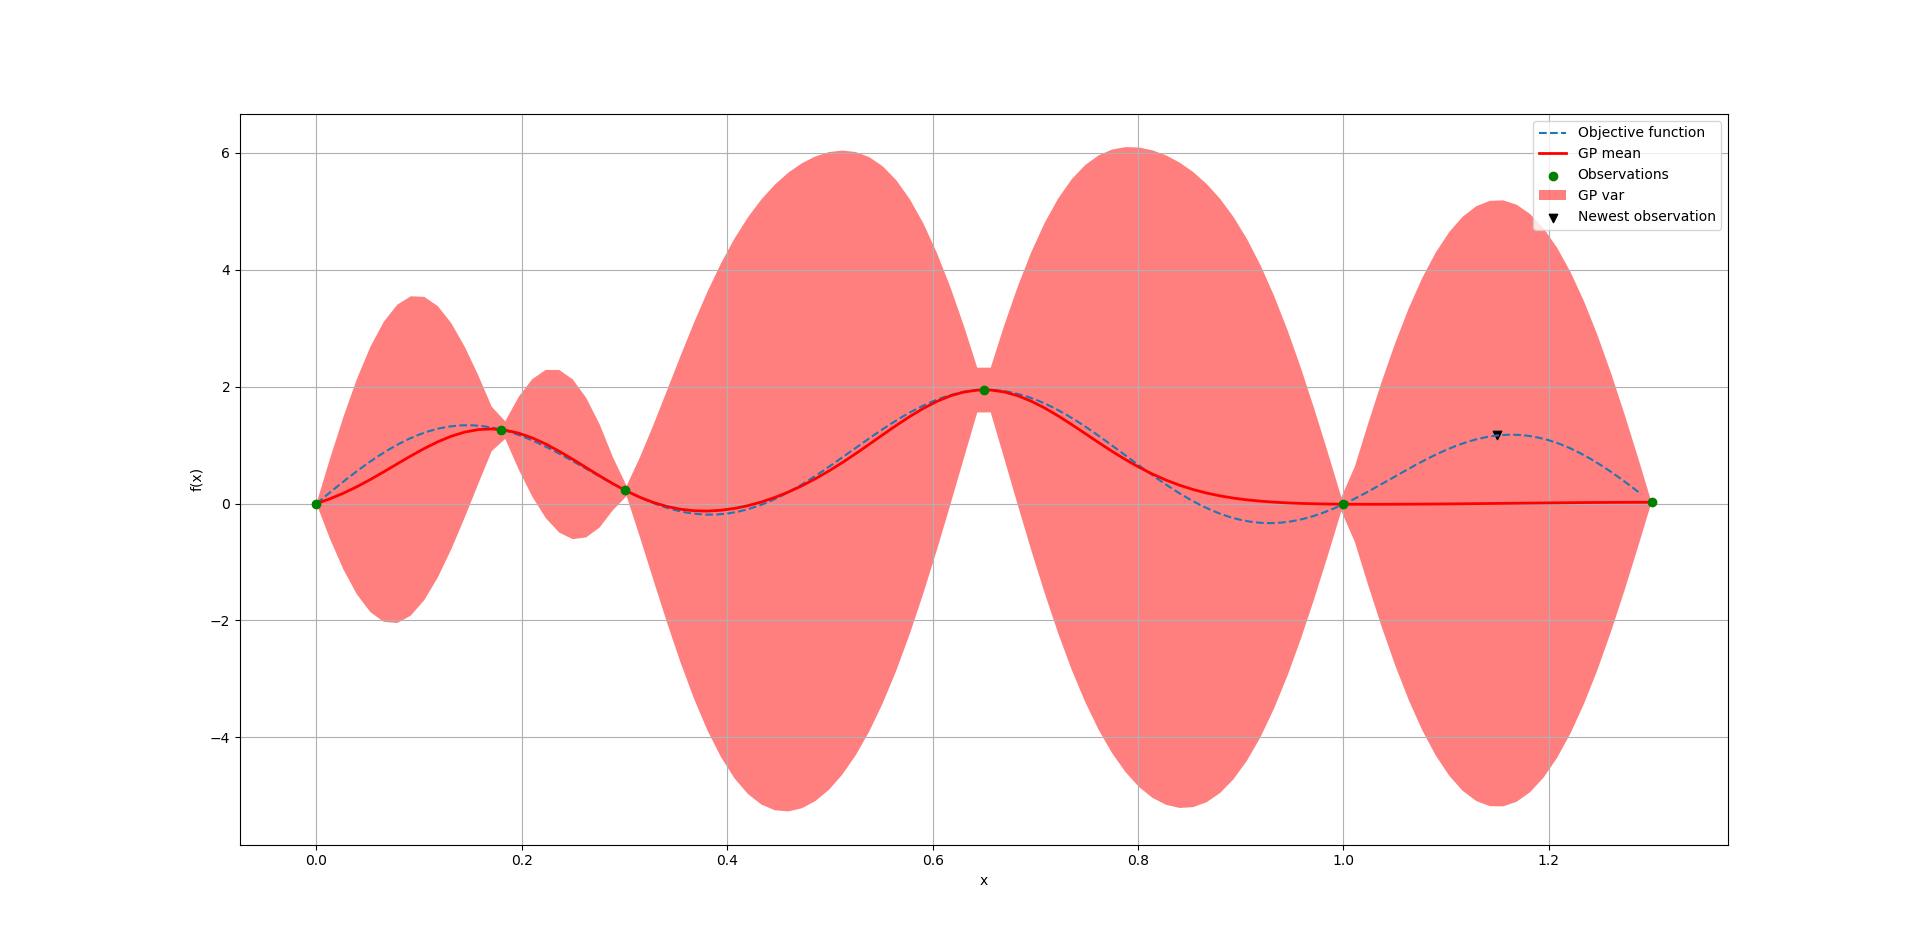
\includegraphics[width=\linewidth]{images/intro_images/BOLoop_4.png}}
%    \only<5>{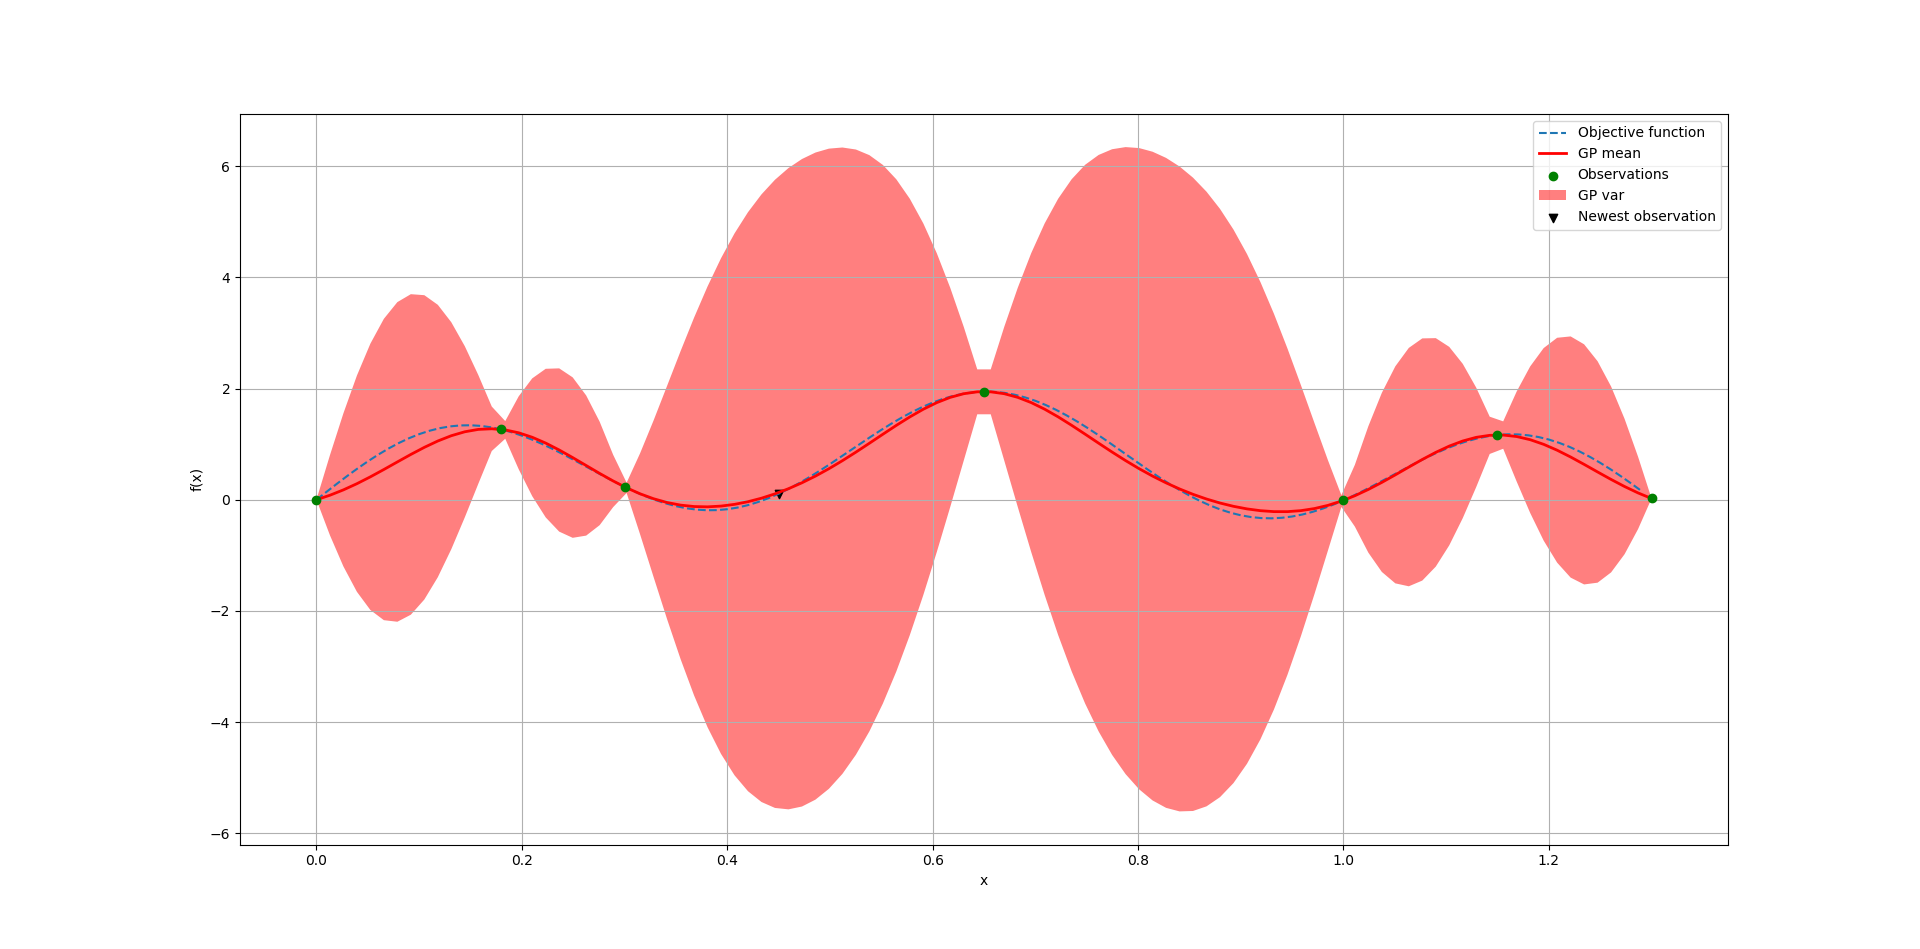
\includegraphics[width=\linewidth]{images/intro_images/BOLoop_5.png}}
%    \only<6>{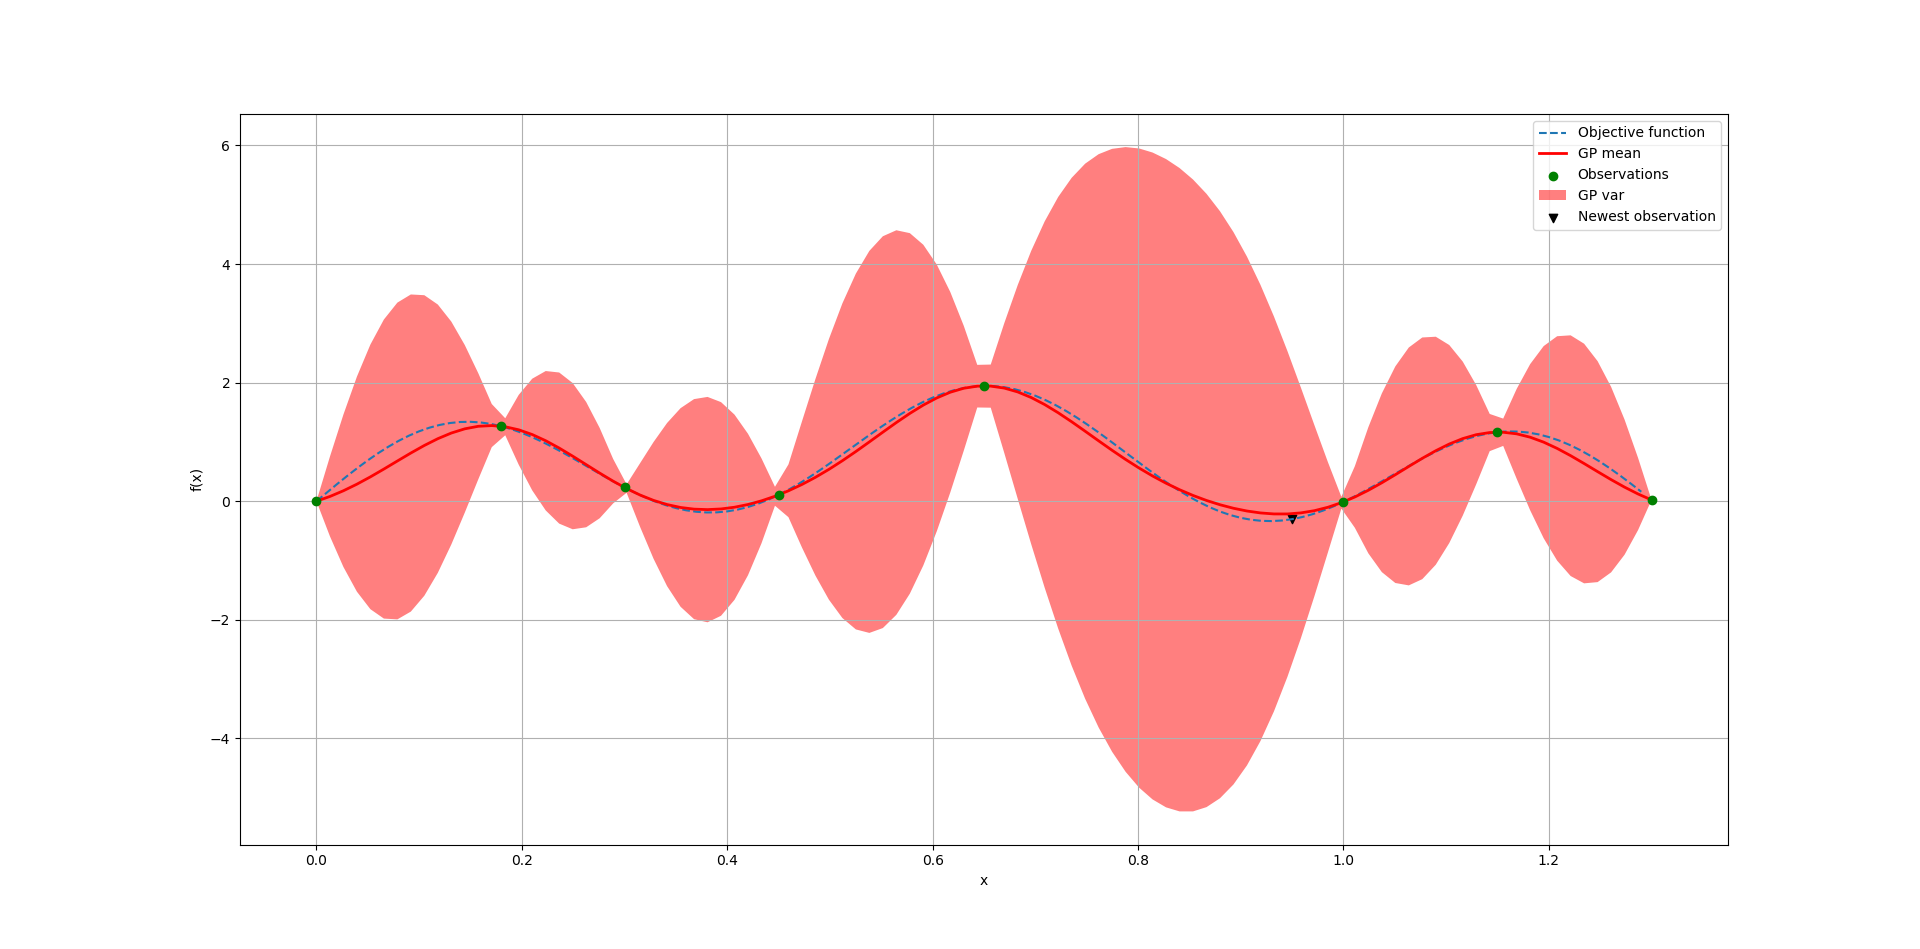
\includegraphics[width=\linewidth]{images/intro_images/BOLoop_6.png}}
%    \only<7>{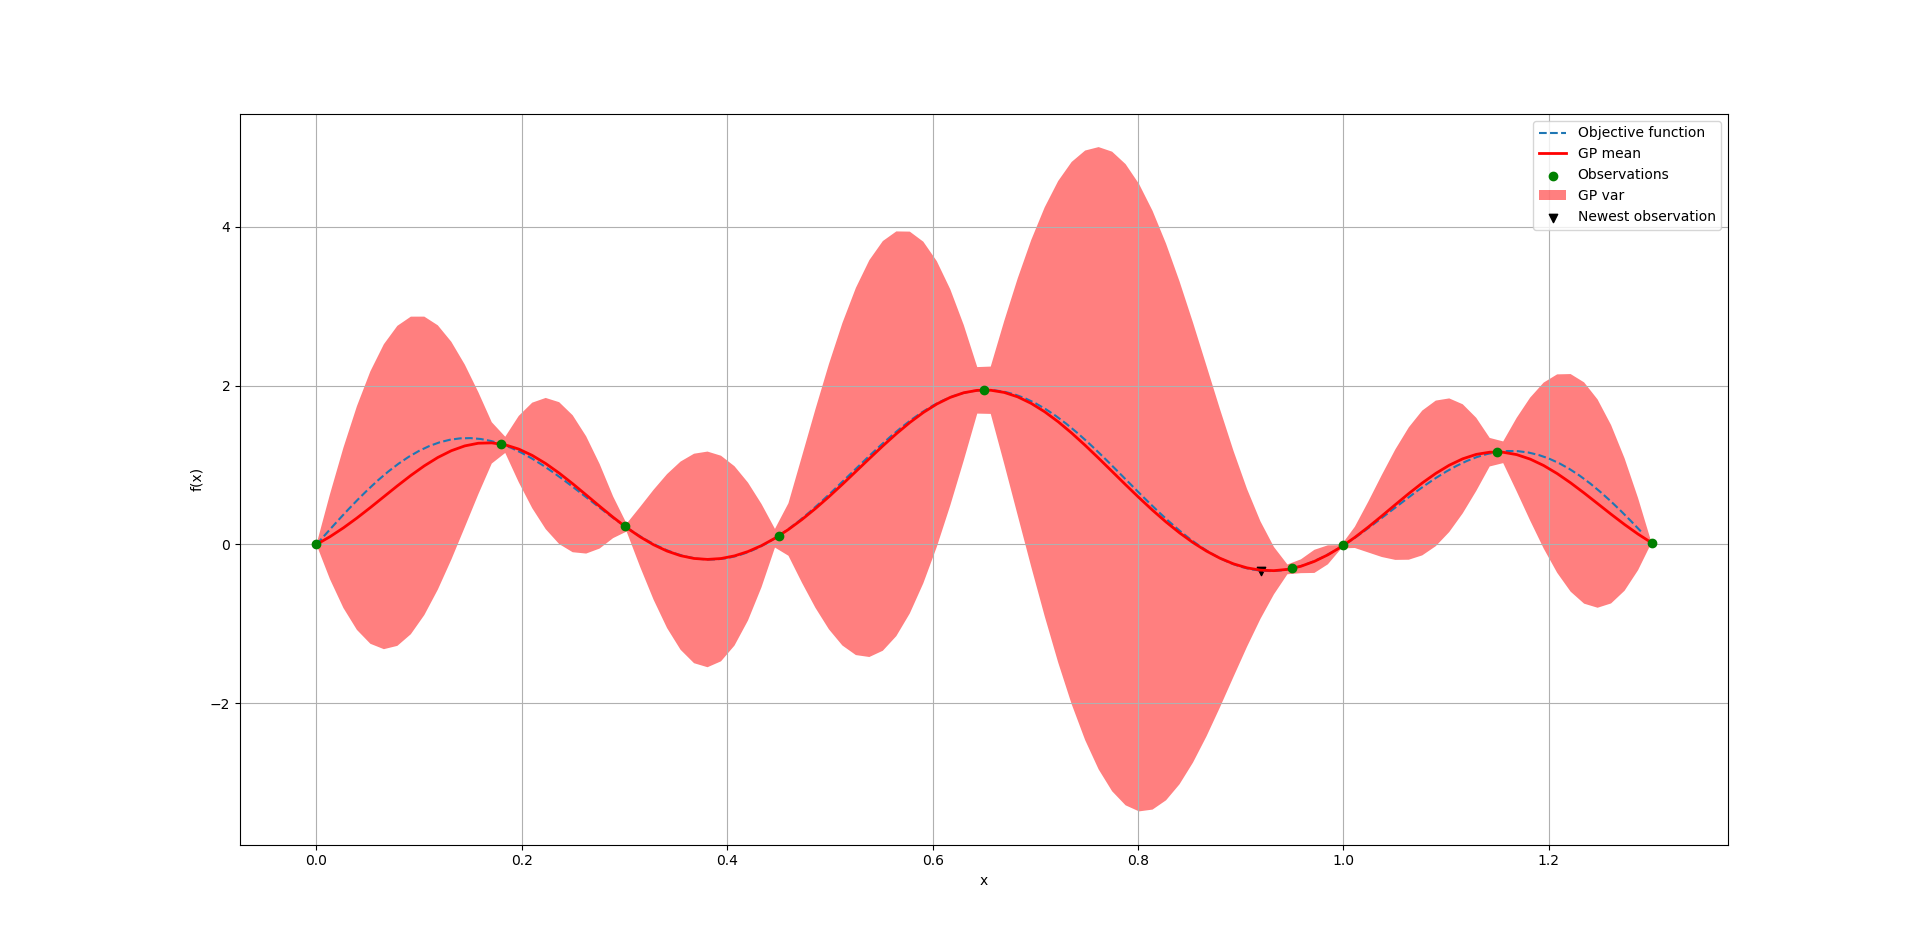
\includegraphics[width=\linewidth]{images/intro_images/BOLoop_7.png}}
%    \only<8>{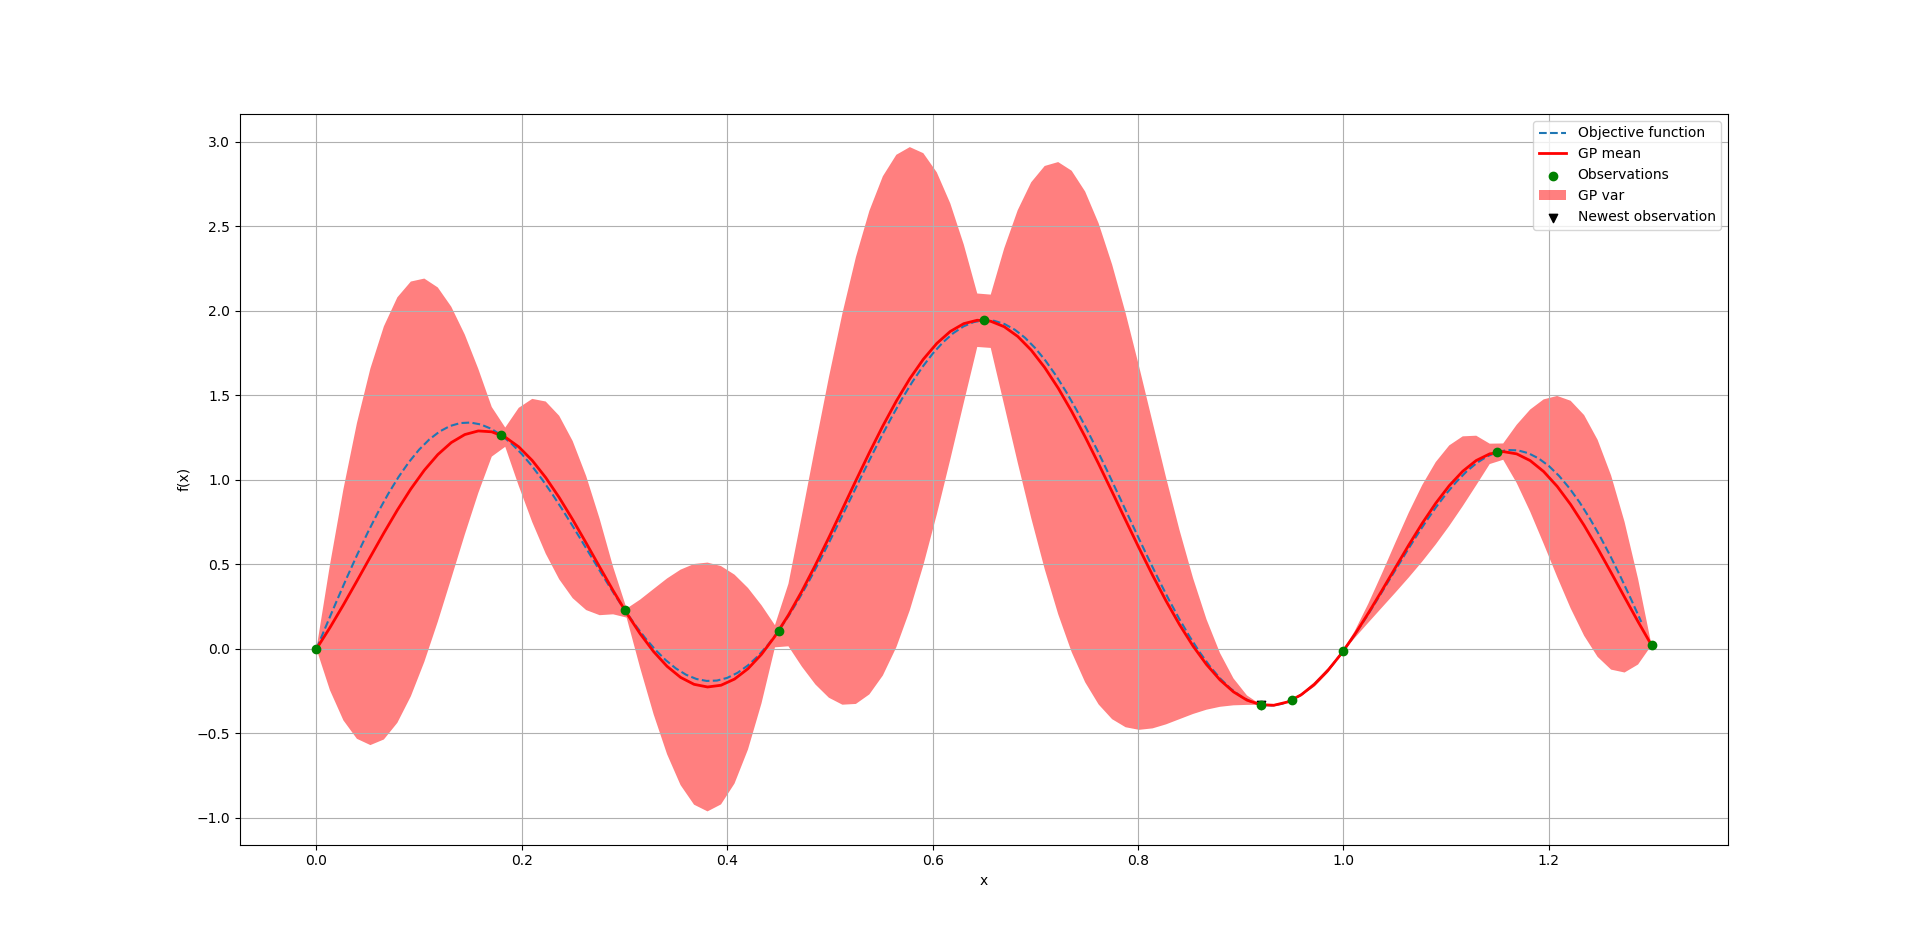
\includegraphics[width=\linewidth]{images/intro_images/BOLoop_8.png}}
%\end{figure}
%\end{frame}
%----------------------------------------------------------------------

\begin{frame}[c]{Bayesian Optimization: Pseudocode}

\begin{center}
\begin{minipage}{0.75\textwidth}
\begin{algorithm}[H]
    %\DontPrintSemicolon
%    \SetAlgoLined
    \setcounter{AlgoLine}{0}
    \SetKwInOut{Require}{Require}
    \SetKwInOut{Result}{Result}
    
    \Require{Search space $\pcs$, 
    		cost function $\cost$, 
    		acquisition function $\acq$, predictive model $\surro$,
    		maximal number of function evaluations $\bobudget$}
    \Result{Best configuration $\finconf$
    (according to $\dataset$ or 
    $\surro$)}
    
	Initialize data $\iter[0]{\dataset}$ with initial observations\;% \leftarrow \varnothing$\; 
	 
    \For{$\bocount=1$ \KwTo $\bobudget$}{
		%\While{$B$ not exhausted} {
		Fit predictive model $\iter[\bocount]{\surro}$ on $\iter[\bocount-1]{\dataset}$\;
		
		Select next query point: $\bonextsample \in \argmax_{\conf \in \pcs} \acq(\conf; \iter[\bocount-1]{\dataset}, \iter[\bocount]{\surro})$\;
		
		Query $\bonextobs$\;
		
		Update data: $\iter[\bocount]{\dataset} \leftarrow \iter[\bocount-1]{\dataset} \cup \{\langle \bonextsample, \bonextobs \rangle \}$\;
	}
	\caption*{BO loop}
\end{algorithm}
\end{minipage}
\end{center}
\end{frame}
%-----------------------------------------------------------------------
\begin{frame}[c]{Bayesian Optimization: Origin of the Name}

\begin{itemize}
    \item Bayesian optimization uses \alert{Bayes' theorem}: 
    	\begin{equation*}
    	    P(A \vert B) = \frac{P(B \vert A) \times  P(A)}{P(B)}
    	    \propto P(B \vert A) \times  P(A)
    	\end{equation*} 
    \item Bayesian optimization uses this to compute a posterior over functions: 
        \begin{equation*}
            P(\func \vert \dataset_{1:\bocount}) \propto P(\dataset_{1:\bocount} \vert \func) \times P(\func), \text{~~~~ where } \dataset_{1:\bocount} = \left \{ \conf_{1:\bocount}, \cost(\conf_{1:\bocount}) \right\}
        \end{equation*} 
\pause
\vspace*{-0.5cm}
    \item Meaning of the individual terms:
        \begin{itemize}
            \item $P(f)$ is the \alert{prior} over functions, which represents our belief about the space of possible objective functions \alert{before} we see any data
            \item $\dataset_{1:\bocount}$ is the \alert{data} (or observations, evidence)
            \item $P(\dataset_{1:\bocount} \vert \func)$ is the likelihood of the data given a function
            \item $P(\func \vert \dataset_{1:\bocount})$ is the \alert{posterior} probability over functions given the data
        \end{itemize}
    \end{itemize}
\end{frame}
%-----------------------------------------------------------------------
\begin{frame}[c]{Bayesian Optimization: Advantages and Disadvantages}

\begin{columns}[T] % align columns
\begin{column}{.48\textwidth}


\begin{block}{Advantages}
\begin{itemize}
  \item Sample efficient 
  \item Can handle noise
  \item Native incorporation of priors 
  \item Does not require gradients 
  \item Theoretical guarantees
\end{itemize}
\end{block}

\end{column}%

\hfill%
\pause 
\begin{column}{.48\textwidth}

\begin{block}{Disadvantages}
\begin{itemize}
  \item Overhead because of model training in each iteration 
  \item Crucially relies on robust surrogate model
  \item Inherently sequential (in its basic form)
\end{itemize}
\end{block}

\end{column}
\end{columns}

\end{frame}
%-----------------------------------------------------------------------
\begin{frame}[c]{Learning Goals of this Lecture}
\framesubtitle{After this lecture, students can ...}

\begin{itemize}
    \item Explain the basics of Bayesian optimization
    \item Derive \alert{simple acquisition functions}
    \item Describe \alert{advanced acquisition functions}
    \item Describe possible \alert{surrogate models} and their pros and cons 
    \item Discuss the \alert{limits of Bayesian optimization} and extensions to tackle these
%    \item Describe the \alert{alternative Bayesian optimization approach of TPE}
    \item Discuss \alert{success stories} of Bayesian optimization
\end{itemize}

\end{frame}

%-----------------------------------------------------------------------
%----------------------------------------------------------------------
%\begin{frame}[c]{Surrogate modelling}
%\framesubtitle{General idea}
%\begin{itemize}
%    \item Use a surrogate model of the expensive function $\cost$ as a cheap-to-evaluate proxy.
%    \begin{itemize}
%        \item Use a probabilistic model with well-calibrated uncertainty predictions.
%    \end{itemize}
%    \pause
%    \item Define a utility function to guide the search for new data points.
%    \pause
%    \item Use the optimization of the utility function as a decision procedure to provide inference on where to evaluate next.
%
%\end{itemize}
%\end{frame}

%-----------------------------------------------------------------------

%\end{document}
    \pdfminorversion=4 % for acroread
%\documentclass[aspectratio=169,t,xcolor={usenames,dvipsnames}]{beamer}
\documentclass[aspectratio=169,t,handout,xcolor={usenames,dvipsnames}]{beamer}
\usepackage{../beamerstyle}
\usepackage{dsfont}
\usepackage{bm}
\usepackage[english]{babel}
\usepackage[utf8]{inputenc}
\usepackage{graphicx}
\usepackage{algorithm}
\usepackage[ruled,vlined,algo2e,linesnumbered]{algorithm2e}
%\usepackage[boxed,vlined]{algorithm2e}
\usepackage{hyperref}
\usepackage{booktabs}
\usepackage{mathtools}

\usepackage{amsmath,amssymb}
\usepackage{listings}
\lstset{frame=lines,framesep=3pt,numbers=left,numberblanklines=false,basicstyle=\ttfamily\small}

\usepackage{subfig}
\usepackage{multicol}
%\usepackage{appendixnumberbeamer}
%
\usepackage{tcolorbox}

\usepackage{pgfplots}
\usepackage{tikz}
\usetikzlibrary{trees} 
\usetikzlibrary{shapes.geometric}
\usetikzlibrary{positioning,shapes,shadows,arrows,calc,mindmap}
\usetikzlibrary{positioning,fadings,through}
\usetikzlibrary{decorations.pathreplacing}
\usetikzlibrary{intersections}
\usetikzlibrary{positioning,fit,calc,shadows,backgrounds}
\pgfdeclarelayer{background}
\pgfdeclarelayer{foreground}
\pgfsetlayers{background,main,foreground}
\tikzstyle{activity}=[rectangle, draw=black, rounded corners, text centered, text width=8em]
\tikzstyle{data}=[rectangle, draw=black, text centered, text width=8em]
\tikzstyle{myarrow}=[->, thick, draw=black]

% Define the layers to draw the diagram
\pgfdeclarelayer{background}
\pgfdeclarelayer{foreground}
\pgfsetlayers{background,main,foreground}

%\usepackage{listings}
%\lstset{numbers=left,
%  showstringspaces=false,
%  frame={tb},
%  captionpos=b,
%  lineskip=0pt,
%  basicstyle=\ttfamily,
%%  extendedchars=true,
%  stepnumber=1,
%  numberstyle=\small,
%  xleftmargin=1em,
%  breaklines
%}

 
\definecolor{blue}{RGB}{0, 74, 153}

\usetheme{Boadilla}
%\useinnertheme{rectangles}
\usecolortheme{whale}
\setbeamercolor{alerted text}{fg=blue}
\useoutertheme{infolines}
\setbeamertemplate{navigation symbols}{\vspace{-5pt}} % to lower the logo
\setbeamercolor{date in head/foot}{bg=white} % blue
\setbeamercolor{date in head/foot}{fg=white}
\setbeamercolor{author  in head/foot}{bg=white} %blue
\setbeamercolor{title in head/foot}{bg=white} % blue
\setbeamercolor{title}{fg=white, bg=blue}
\setbeamercolor{block title}{fg=white,bg=blue}
\setbeamercolor{block body}{bg=blue!10}
\setbeamercolor{frametitle}{fg=white, bg=blue}
\setbeamercovered{invisible}

\makeatletter
\setbeamertemplate{footline}
{
  \leavevmode%
  \hbox{%
  \begin{beamercolorbox}[wd=.333333\paperwidth,ht=2.25ex,dp=1ex,center]{author in head/foot}%
%    \usebeamerfont{author in head/foot}\insertshortauthor
  \end{beamercolorbox}%
  \begin{beamercolorbox}[wd=.333333\paperwidth,ht=2.25ex,dp=1ex,center]{title in head/foot}%
    \usebeamerfont{title in head/foot}\insertshorttitle
  \end{beamercolorbox}%
  \begin{beamercolorbox}[wd=.333333\paperwidth,ht=2.25ex,dp=1ex,right]{date in head/foot}%
    \usebeamerfont{date in head/foot}\insertshortdate{}\hspace*{2em}
%    \insertframenumber\hspace*{2ex} 
  \end{beamercolorbox}}%
  \vskip0pt%
}
\makeatother

%\pgfdeclareimage[height=1.2cm]{automl}{images/logos/automl.png}
%\pgfdeclareimage[height=1.2cm]{freiburg}{images/logos/freiburg}

%\logo{\pgfuseimage{freiburg}}

\renewcommand{\comment}[1]{
	\noindent
	%\vspace{0.25cm}
	{\color{red}{\textbf{TODO:} #1}}
	%\vspace{0.25cm}
}
\newcommand{\notefh}[1]{\textcolor{red}{\textbf{FH:} #1}}
\renewcommand{\comment}[1]{}
\newcommand{\hide}[1]{}
\newcommand{\cemph}[2]{\emph{\textcolor{#1}{#2}}}

\newcommand{\lit}[1]{{\footnotesize\color{black!60}[#1]}}

\newcommand{\litw}[1]{{\footnotesize\color{blue!20}[#1]}}


\newcommand{\myframe}[2]{\begin{frame}[c]{#1}#2\end{frame}}
\newcommand{\myframetop}[2]{\begin{frame}{#1}#2\end{frame}}
\newcommand{\myit}[1]{\begin{itemize}#1\end{itemize}}
\newcommand{\myblock}[2]{\begin{block}{#1}#2\end{block}}


\newcommand{\votepurple}[1]{\textcolor{Purple}{$\bigstar$}}
\newcommand{\voteyellow}[1]{\textcolor{Goldenrod}{$\bigstar$}}
\newcommand{\voteblue}[1]{\textcolor{RoyalBlue}{$\bigstar$}}
\newcommand{\votepink}[1]{\textcolor{Pink}{$\bigstar$}}

\newcommand{\diff}{\mathop{}\!\mathrm{d}}
\newcommand{\refstyle}[1]{{\small{\textcolor{gray}{#1}}}}
\newcommand{\hands}[0]{
\includegraphics[height=1.5em]{images/hands}}
\newcommand{\transpose}[0]{{\textrm{\tiny{\sf{T}}}}}
\newcommand{\norm}{{\mathcal{N}}}
\newcommand{\cutoff}[0]{\kappa}
\newcommand{\instD}[0]{\dataset}
\newcommand{\insts}[0]{\mathcal{I}}
\newcommand{\inst}[0]{i}
\newcommand{\instI}[1]{i^{(#1)}}

% Iteration specific instance of variable/function/anything
% Introduced in the BO section, but moved up here to make it available within other macros
\newcommand{\iter}[2][\bocount]{{#2}^{(#1)}}

%--------HPO parameter macros-----------

% Parameter Configuration Space
\newcommand{\pcs}[0]{\pmb{\Lambda}}

% ???
\newcommand{\bx}[0]{\conf}

% Parameter Configuration
\newcommand{\conf}[0]{\pmb{\lambda}}

% Final Configuration
\newcommand{\finconf}[0]{\pmb{\hat{\lambda}}}

% Configuration corresponding to a given iteration -- better use \iter!
\newcommand{\confI}[1]{{\conf}^{(#1)}}

% Default Configuration
\newcommand{\defconf}[0]{{\conf}_{\text{def}}}

% Incumbent Configuration
\newcommand{\incumbent}[1][\bocount]{\iter[#1]{\finconf}}

% Optimal Configuration
\newcommand{\optconf}[0]{{\conf}^*}

% Configuration Space
\newcommand{\confs}[0]{\pcs}

%----------------------------------------

%\newcommand{\vlambda}[0]{\bm{\lambda}}
%\newcommand{\vLambda}[0]{\bm{\Lambda}}
\newcommand{\dataset}[0]{\mathcal{D}}
\newcommand{\datasets}[0]{\mathbf{D}}
\newcommand{\loss}[0]{L}
\newcommand{\risk}{\mathcal{R}}
\newcommand{\riske}{\mathcal{R}_{\text{emp}}}
\newcommand{\cost}[0]{c}
\newcommand{\costI}[1]{c^{(#1)}}

% Gaussian Process
\newcommand{\gp}{\mathcal{G}}
% Family of Objective Functions
\newcommand{\objF}{F}

%---------------BO Macros------------------

% BO loop counter
\newcommand{\bocount}{t}
% BO loop counter max, the counter runs from 1 to this value
\newcommand{\bobudget}{T}
% BO loop observation
\newcommand{\obs}[1][\conf]{\cost({#1})}
% BO loop observation space
\newcommand{\obsspace}{\mathcal{Y}}
% BO loop next observation
\newcommand{\bonextobs}{\obs[\iter{\conf}]}
% Acquisition Function, no args
\newcommand{\acq}{u}
% Standard Normal PDF
\newcommand{\pdf}{\phi}
% Standard Normal CDF
\newcommand{\cdf}{\Phi}
% Mean
\newcommand{\mean}{\mu}
% Standard Deviation
\newcommand{\stddev}{\sigma}
% Variance
\newcommand{\variance}{\sigma^2}
% Noise
\newcommand{\noise}{\nu}
% BO loop next selected sample
\newcommand{\bonextsample}{\confI{\bocount}}

% Single hyperparameter
\newcommand{\hyperparam}{\lambda}

% Single hyperparameter within a hyperparameter configuration
\newcommand{\hyperparami}[1][i]{{\hyperparam}_#1}

% Full definition of final configuration
\newcommand{\finconffull}{\incumbent[\bobudget]}

% Dataset
\newcommand{\datasetHPO}{{\dataset}_{HPO}}

% Dataset definition
\newcommand{\datasetHPOdef}{{\langle \bonextsample,\,\bonextobs \rangle}_{\bocount=1}^{\bobudget}}

% Double Display Fraction, forces large displays for everything in numerator and denominator
\newcommand\ddfrac[2]{\frac{\displaystyle #1}{\displaystyle #2}}

% Conditional Probability "Given That" Relation, source:https://tex.stackexchange.com/a/141685/205886
\newcommand\given[1][]{\:#1\vert\:}

% Expectation as a math operator
\DeclareMathOperator*{\E}{\mathbb{E}}

% Citation 
\newcommand{\source}[1]{
    \begin{flushright}
    	Source: \lit{#1}
    \end{flushright}
}
%-------------------------------------------

%Real numbers set
\newcommand{\realnum}{\mathbb{R}}
%Configuration space - do not use
%\newcommand{\configspace}{\Theta}
%Instances - do not use
%\newcommand{\instances}{\mathcal{I}}
%Expected value
\newcommand{\expectation}{\mathbb{E}}
%Kernel
\newcommand{\kernel}{\kappa}
%Constraint function
\newcommand{\constraintf}{c}
%Normal distribution
\newcommand{\normaldist}{\mathcal{N}}

% \renewcommand{\vec}[1]{\mathbf{#1}}
\newcommand{\hist}[0]{\dataset_{\text{Hist}}}
\newcommand{\param}[0]{p}
\newcommand{\algo}[0]{\mathcal{A}}
\newcommand{\algos}[0]{\mathbf{A}}
%\newcommand{\nn}[0]{N}
\newcommand{\feats}[0]{\mathcal{X}_{\text{meta}}}
\newcommand{\feat}[0]{\x_{\text{meta}}}
%\newcommand{\cluster}[0]{\vec{h}}
%\newcommand{\clusters}[0]{\vec{H}}
\newcommand{\perf}[0]{\mathbb{R}}
%\newcommand{\surro}[0]{\mathcal{S}}
\newcommand{\surro}[0]{\hat{\cost}}
\newcommand{\func}[0]{f}
\newcommand{\epm}[0]{\surro}
\newcommand{\portfolio}[0]{\mathbf{P}}
\newcommand{\schedule}[0]{\mathcal{S}}

% Machine Learning
\newcommand{\mdata}[0]{\dataset_{\text{meta}}}
\newcommand{\datasettrain}[0]{\dataset_{\text{train}}}
\newcommand{\datasetval}[0]{\dataset_{\text{val}}}
\newcommand{\datasettest}[0]{\dataset_{\text{test}}}
\newcommand{\x}[0]{\mathbf{x}}
\newcommand{\y}[0]{y}
\newcommand{\xI}[1]{\mathbf{x}^{(#1)}}
\newcommand{\yI}[1]{y^{(#1)}}
\newcommand{\fx}{f(\mathbf{x})}  % f(x), continuous prediction function
\newcommand{\Hspace}{\mathcal{H}} % hypothesis space where f is from
\newcommand{\fh}{\hat{f}}       % f hat, estimated prediction function

% Deep Learning
\newcommand{\weights}[0]{\theta}
\newcommand{\metaweights}[0]{\phi}


% reinforcement learning
\newcommand{\policies}[0]{\mathbf{\Pi}}
\newcommand{\policy}[0]{\pi}
\newcommand{\actionRL}[0]{a}
\newcommand{\stateRL}[0]{s}
\newcommand{\statesRL}[0]{\mathcal{S}}
\newcommand{\rewardRL}[0]{r}
\newcommand{\rewardfuncRL}[0]{\mathcal{R}}

\RestyleAlgo{algoruled}
\DontPrintSemicolon
\LinesNumbered
\SetAlgoVlined
\SetFuncSty{textsc}

\SetKwInOut{Input}{Input}
\SetKwInOut{Output}{Output}
\SetKw{Return}{return}

%\newcommand{\changed}[1]{{\color{red}#1}}

%\newcommand{\citeN}[1]{\citeauthor{#1}~(\citeyear{#1})}

\renewcommand{\vec}[1]{\mathbf{#1}}
\DeclareMathOperator*{\argmin}{arg\,min}
\DeclareMathOperator*{\argmax}{arg\,max}

%\newcommand{\aqme}{\textit{AQME}}
%\newcommand{\aslib}{\textit{ASlib}}
%\newcommand{\llama}{\textit{LLAMA}}
%\newcommand{\satzilla}{\textit{SATzilla}}
%\newcommand{\satzillaY}[1]{\textit{SATzilla'{#1}}}
%\newcommand{\snnap}{\textit{SNNAP}}
%\newcommand{\claspfolioTwo}{\textit{claspfolio~2}}
%\newcommand{\flexfolio}{\textit{FlexFolio}}
%\newcommand{\claspfolioOne}{\textit{claspfolio~1}}
%\newcommand{\isac}{\textit{ISAC}}
%\newcommand{\eisac}{\textit{EISAC}}
%\newcommand{\sss}{\textit{3S}}
%\newcommand{\sunny}{\textit{Sunny}}
%\newcommand{\ssspar}{\textit{3Spar}}
%\newcommand{\cshc}{\textit{CSHC}}
%\newcommand{\cshcpar}{\textit{CSHCpar}}
%\newcommand{\measp}{\textit{ME-ASP}}
%\newcommand{\aspeed}{\textit{aspeed}}
%\newcommand{\autofolio}{\textit{AutoFolio}}
%\newcommand{\cedalion}{\textit{Cedalion}}
\newcommand{\fanova}{\textit{fANOVA}}
\newcommand{\sbs}{\textit{SB}}
\newcommand{\oracle}{\textit{VBS}}

% like approaches
\newcommand{\claspfoliolike}[1]{\texttt{claspfolio-#1-like}}
\newcommand{\satzillalike}[1]{\texttt{SATzilla'#1-like}}
\newcommand{\isaclike}{\texttt{ISAC-like}}
\newcommand{\ssslike}{\texttt{3S-like}}
\newcommand{\measplike}{\texttt{ME-ASP-like}}

\newcommand{\irace}{\textit{I/F-race}}
\newcommand{\gga}{\textit{GGA}}
\newcommand{\smac}{\textit{SMAC}}
\newcommand{\paramils}{\textit{ParamILS}}
\newcommand{\spearmint}{\textit{Spearmint}}
\newcommand{\tpe}{\textit{TPE}}


\usepackage{pifont}
\newcommand{\itarrow}{\mbox{\Pisymbol{pzd}{229}}}
\newcommand{\ithook}{\mbox{\Pisymbol{pzd}{52}}}
\newcommand{\itcross}{\mbox{\Pisymbol{pzd}{56}}}
\newcommand{\ithand}{\mbox{\raisebox{-1pt}{\Pisymbol{pzd}{43}}}}

%\DeclareMathOperator*{\argmax}{arg\,max}

\newcommand{\ie}{{\it{}i.e.\/}}
\newcommand{\eg}{{\it{}e.g.\/}}
\newcommand{\cf}{{\it{}cf.\/}}
\newcommand{\wrt}{\mbox{w.r.t.}}
\newcommand{\vs}{{\it{}vs\/}}
\newcommand{\vsp}{{\it{}vs\/}}
\newcommand{\etc}{{\copyedit{etc.}}}
\newcommand{\etal}{{\it{}et al.\/}}

\newcommand{\pscProc}{{\bf procedure}}
\newcommand{\pscBegin}{{\bf begin}}
\newcommand{\pscEnd}{{\bf end}}
\newcommand{\pscEndIf}{{\bf endif}}
\newcommand{\pscFor}{{\bf for}}
\newcommand{\pscEach}{{\bf each}}
\newcommand{\pscThen}{{\bf then}}
\newcommand{\pscElse}{{\bf else}}
\newcommand{\pscWhile}{{\bf while}}
\newcommand{\pscIf}{{\bf if}}
\newcommand{\pscRepeat}{{\bf repeat}}
\newcommand{\pscUntil}{{\bf until}}
\newcommand{\pscWithProb}{{\bf with probability}}
\newcommand{\pscOtherwise}{{\bf otherwise}}
\newcommand{\pscDo}{{\bf do}}
\newcommand{\pscTo}{{\bf to}}
\newcommand{\pscOr}{{\bf or}}
\newcommand{\pscAnd}{{\bf and}}
\newcommand{\pscNot}{{\bf not}}
\newcommand{\pscFalse}{{\bf false}}
\newcommand{\pscEachElOf}{{\bf each element of}}
\newcommand{\pscReturn}{{\bf return}}

%\newcommand{\param}[1]{{\sl{}#1}}
\newcommand{\var}[1]{{\it{}#1}}
\newcommand{\cond}[1]{{\sf{}#1}}
%\newcommand{\state}[1]{{\sf{}#1}}
%\newcommand{\func}[1]{{\sl{}#1}}
\newcommand{\set}[1]{{\Bbb #1}}
%\newcommand{\inst}[1]{{\tt{}#1}}
\newcommand{\myurl}[1]{{\small\sf #1}}

\newcommand{\Nats}{{\Bbb N}}
\newcommand{\Reals}{{\Bbb R}}
\newcommand{\extset}[2]{\{#1 \; | \; #2\}}

\newcommand{\vbar}{$\,\;|$\hspace*{-1em}\raisebox{-0.3mm}{$\,\;\;|$}}
\newcommand{\vendbar}{\raisebox{+0.4mm}{$\,\;|$}}
\newcommand{\vend}{$\,\:\lfloor$}


\newcommand{\goleft}[2][.7]{\parbox[t]{#1\linewidth}{\strut\raggedright #2\strut}}
\newcommand{\rightimage}[2][.3]{\mbox{}\hfill\raisebox{1em-\height}[0pt][0pt]{\includegraphics[width=#1\linewidth]{#2}}\vspace*{-\baselineskip}}






\title{AutoML: Bayesian Optimization for HPO}
\subtitle{Computationally Cheap Acquisition Functions}
\author[Marius Lindauer]{Bernd Bischl \and \underline{Frank Hutter} \and Lars Kotthoff\newline \and Marius Lindauer \and Joaquin Vanschoren}
\institute{}
\date{}

\begin{document}
\maketitle

%----------------------------------------------------------------------
\begin{frame}[c]{Acquisition Functions: the Basics}
\begin{itemize}
    \item Given the surrogate model $\iter{\surro}$ at the $\bocount$-th iteration of BO, the \\
    \alert{acquisition function $\acq(\cdot)$ judges the utility (or usefulness) of evaluating $f$ at $\iter{\conf}\in \pcs$ next}
    \pause
    \bigskip
    \item The acquisition function needs to \alert{trade off exploration and exploitation}
    \begin{itemize}
        \item E.g., just picking the $\conf$ with lowest predicted mean would be too greedy
        \item We also need to take into account the uncertainty of the surrogate model $\iter{\surro}$ to explore
    \end{itemize}
\end{itemize}

\end{frame}
%-----------------------------------------------------------------------
\begin{frame}[c]{Probability of Improvement (PI): Concept}

  {
    %\framesubtitle{Probability of Improvement - Concept}
    % \begin{figure}
      \centering
      \begin{tikzpicture}
        \node<+> (img1) {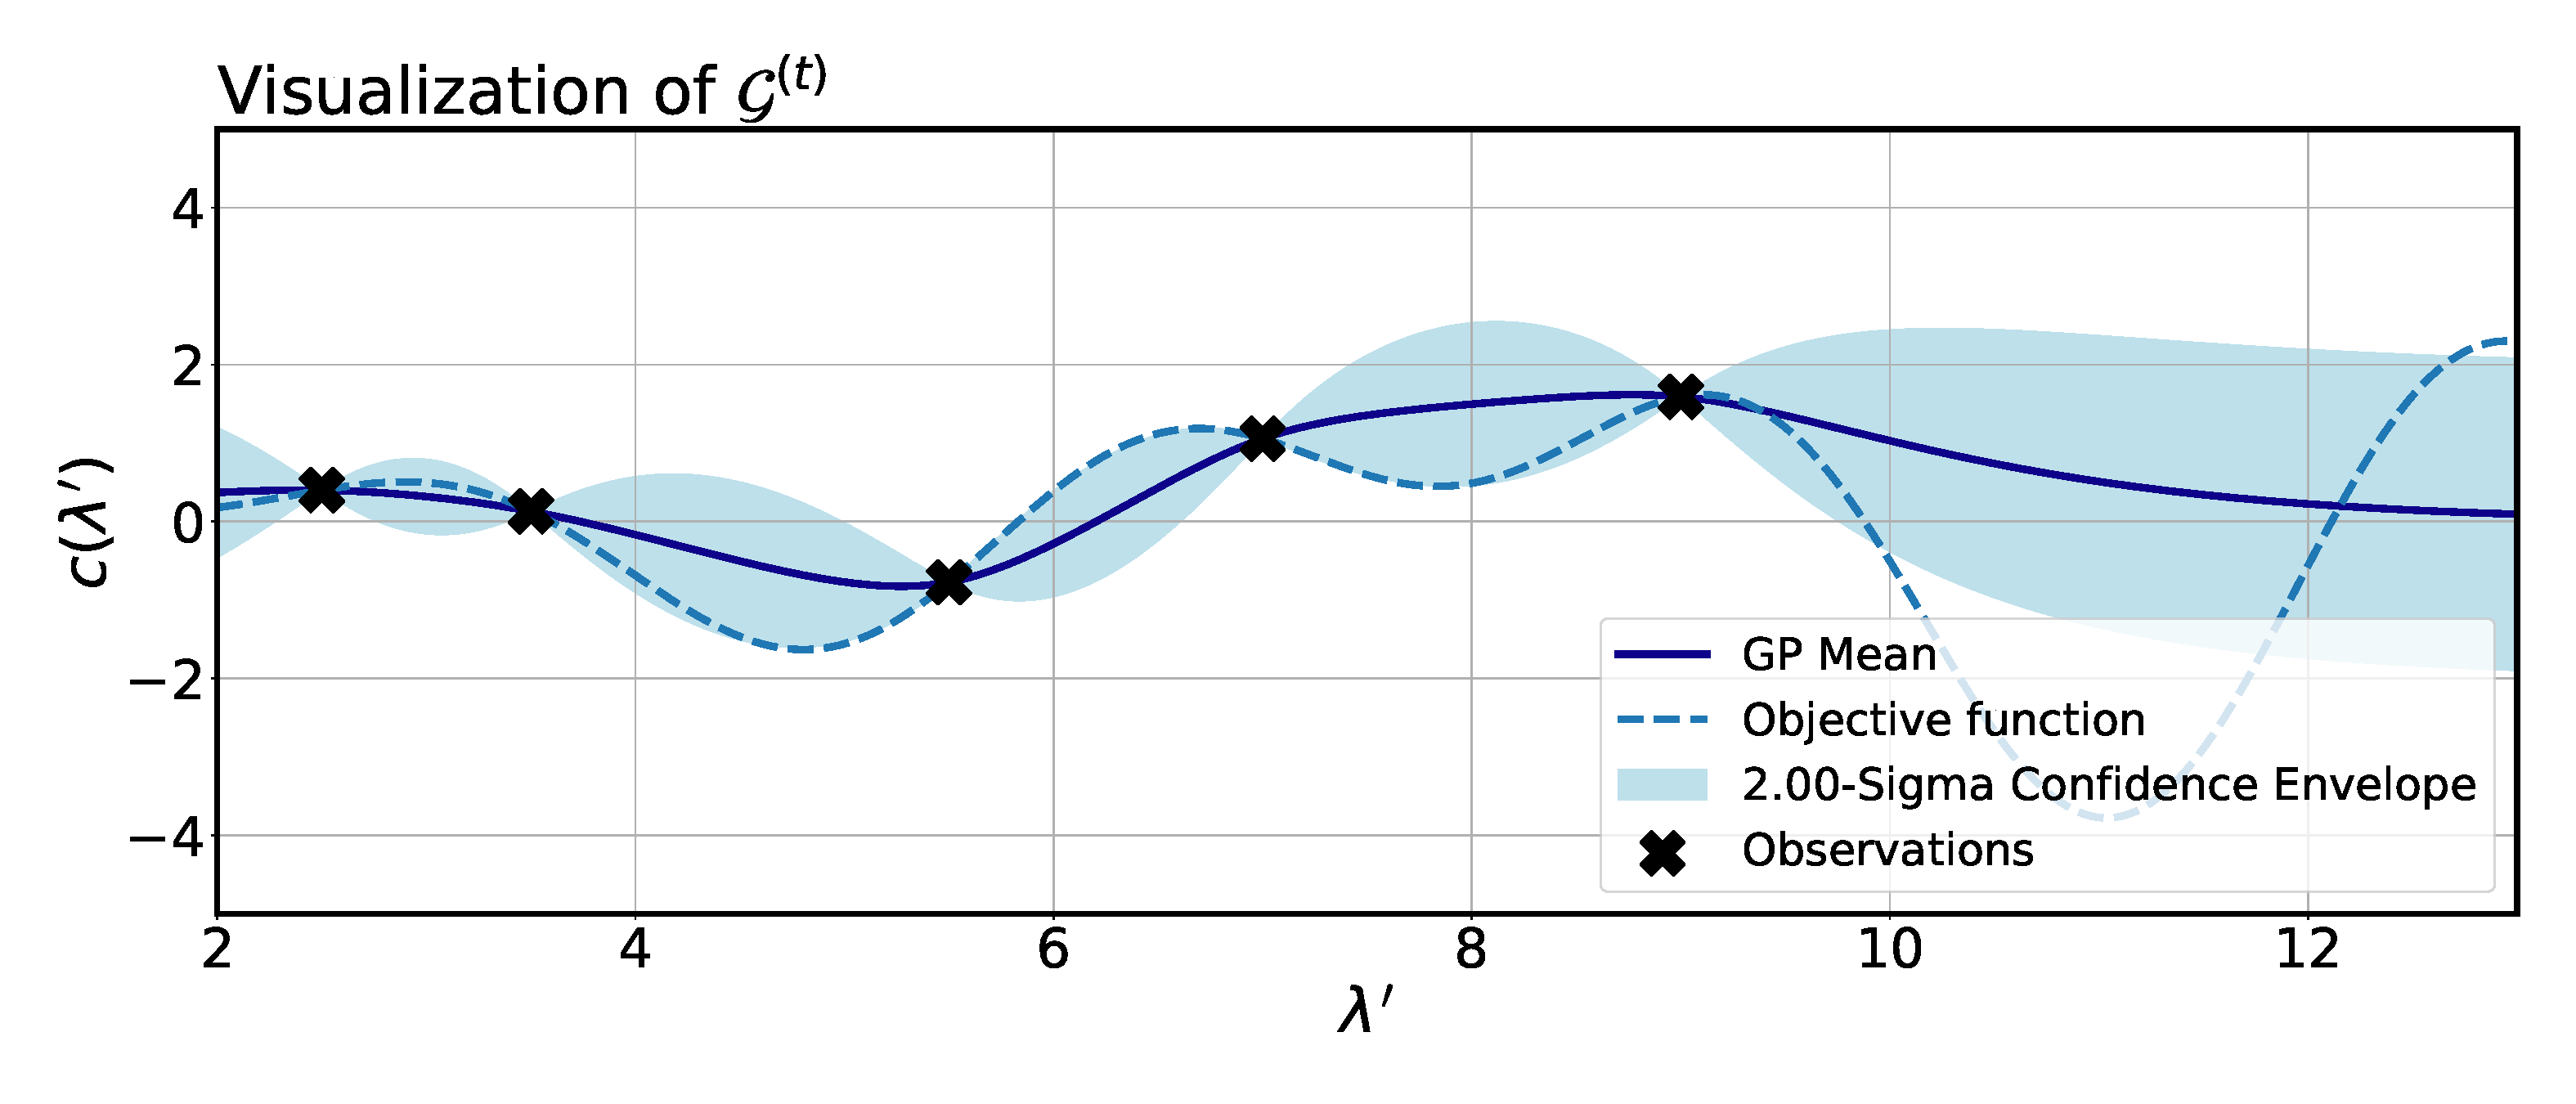
\includegraphics[width=\linewidth, height=0.7\textheight, keepaspectratio=true]{images/acq_func_images/pi/pi_1.pdf}};
        \node<.> [below=0.01\belowcaptionskip of img1, align=center]{Given the surrogate fit at iteration $\bocount$};
    
        \node<+> (img2) {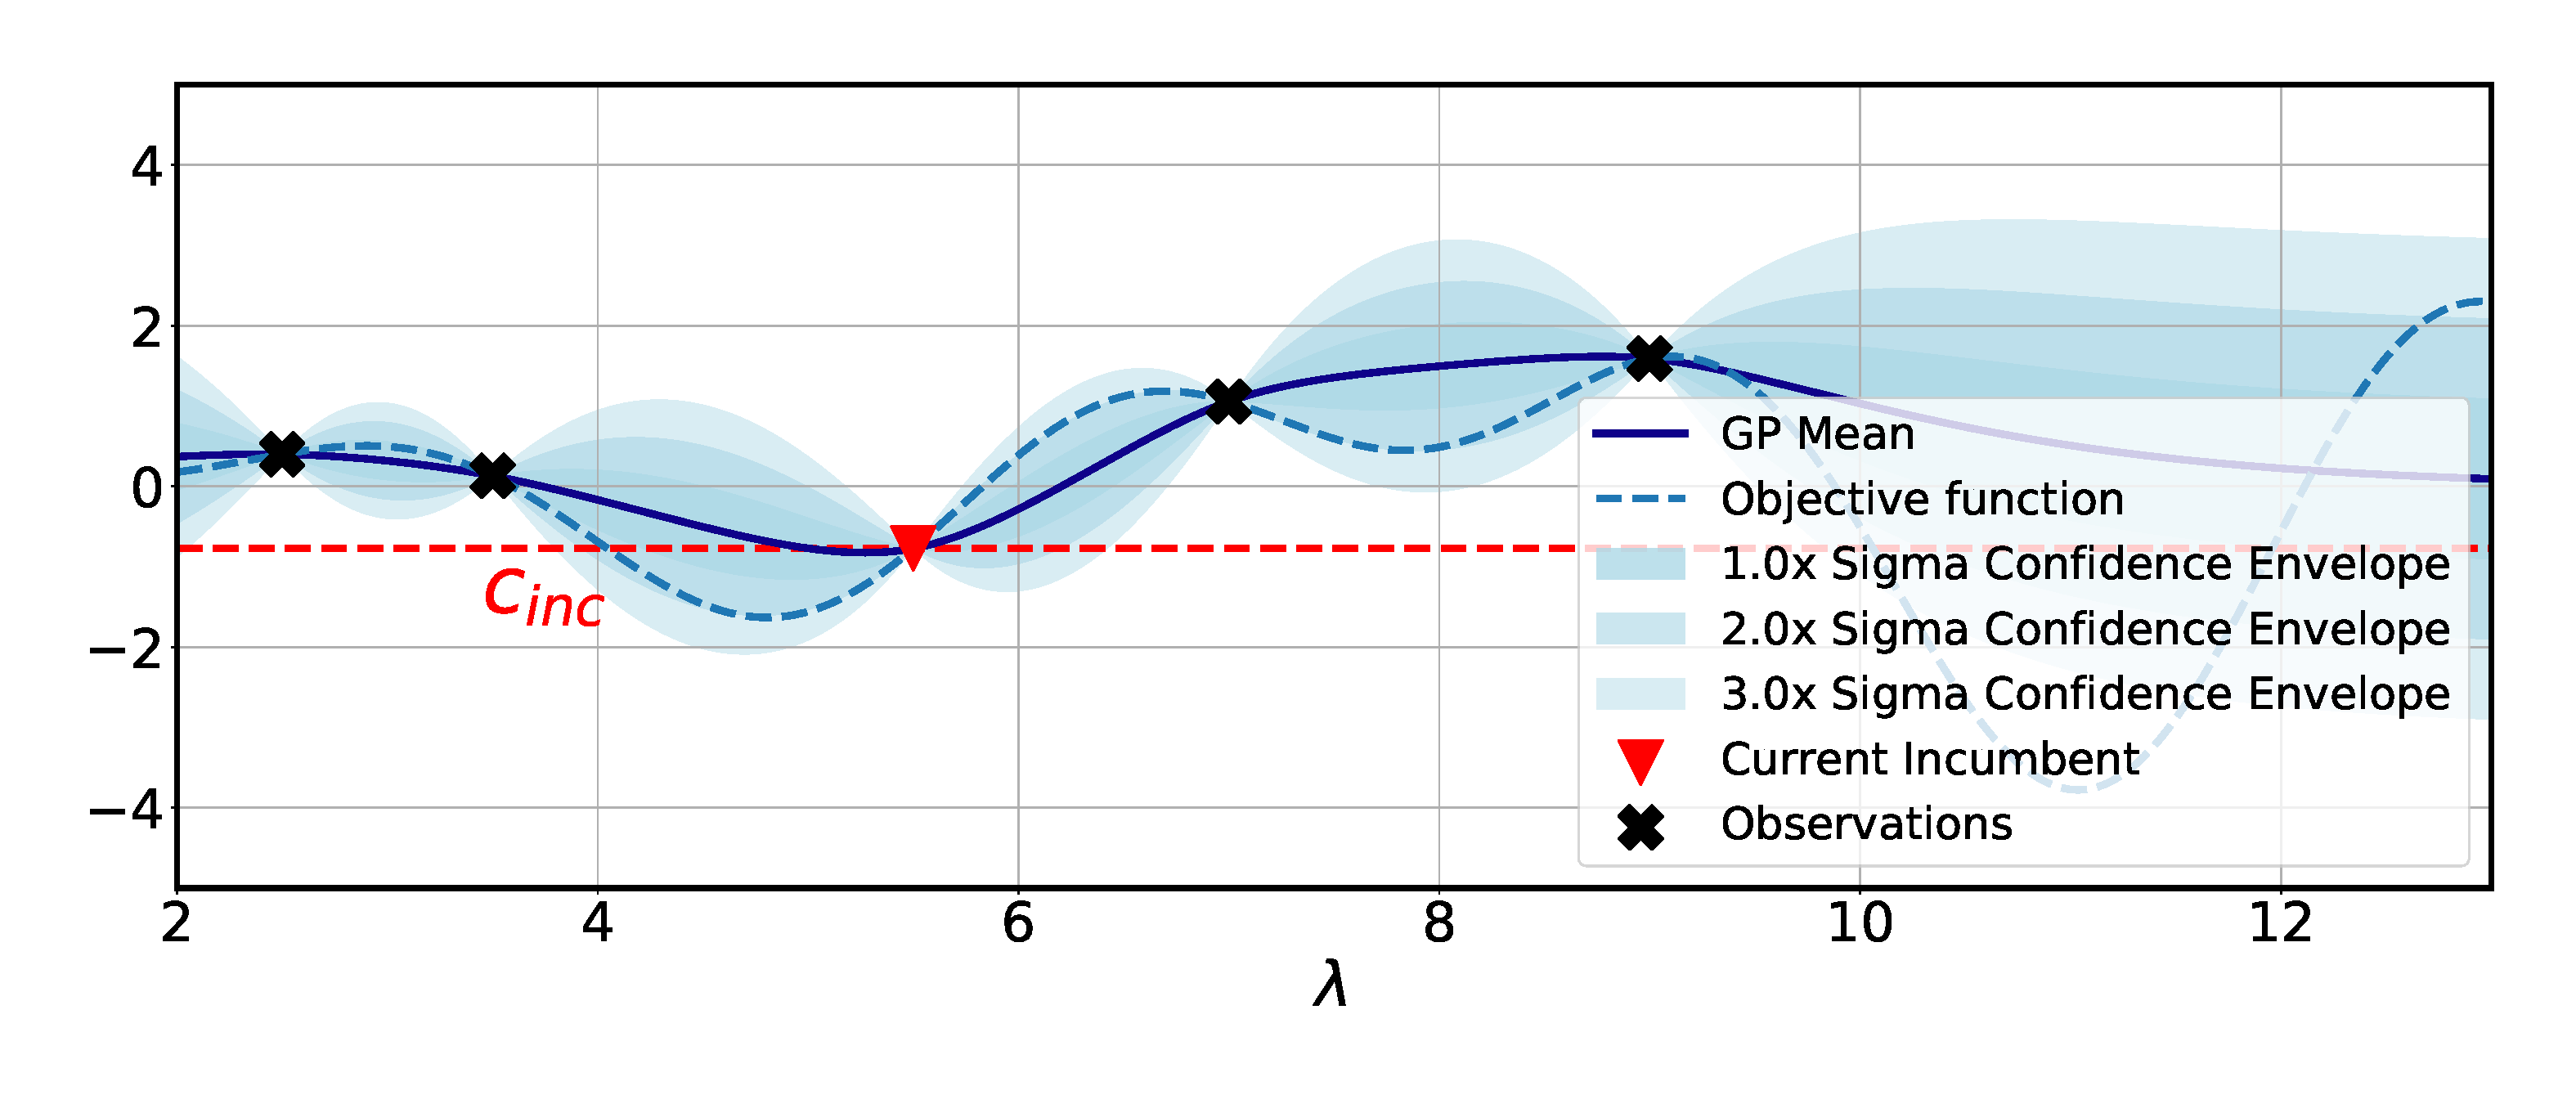
\includegraphics[width=\linewidth, height=0.7\textheight, keepaspectratio=true]{images/acq_func_images/pi/pi_2.pdf}};
        \node<.> [below=0.01\belowcaptionskip of img2, align=center]{Current incumbent $\hat{\conf}$ and its observed cost $\cost_{inc}$};
    
    
        \node<+> (img3) {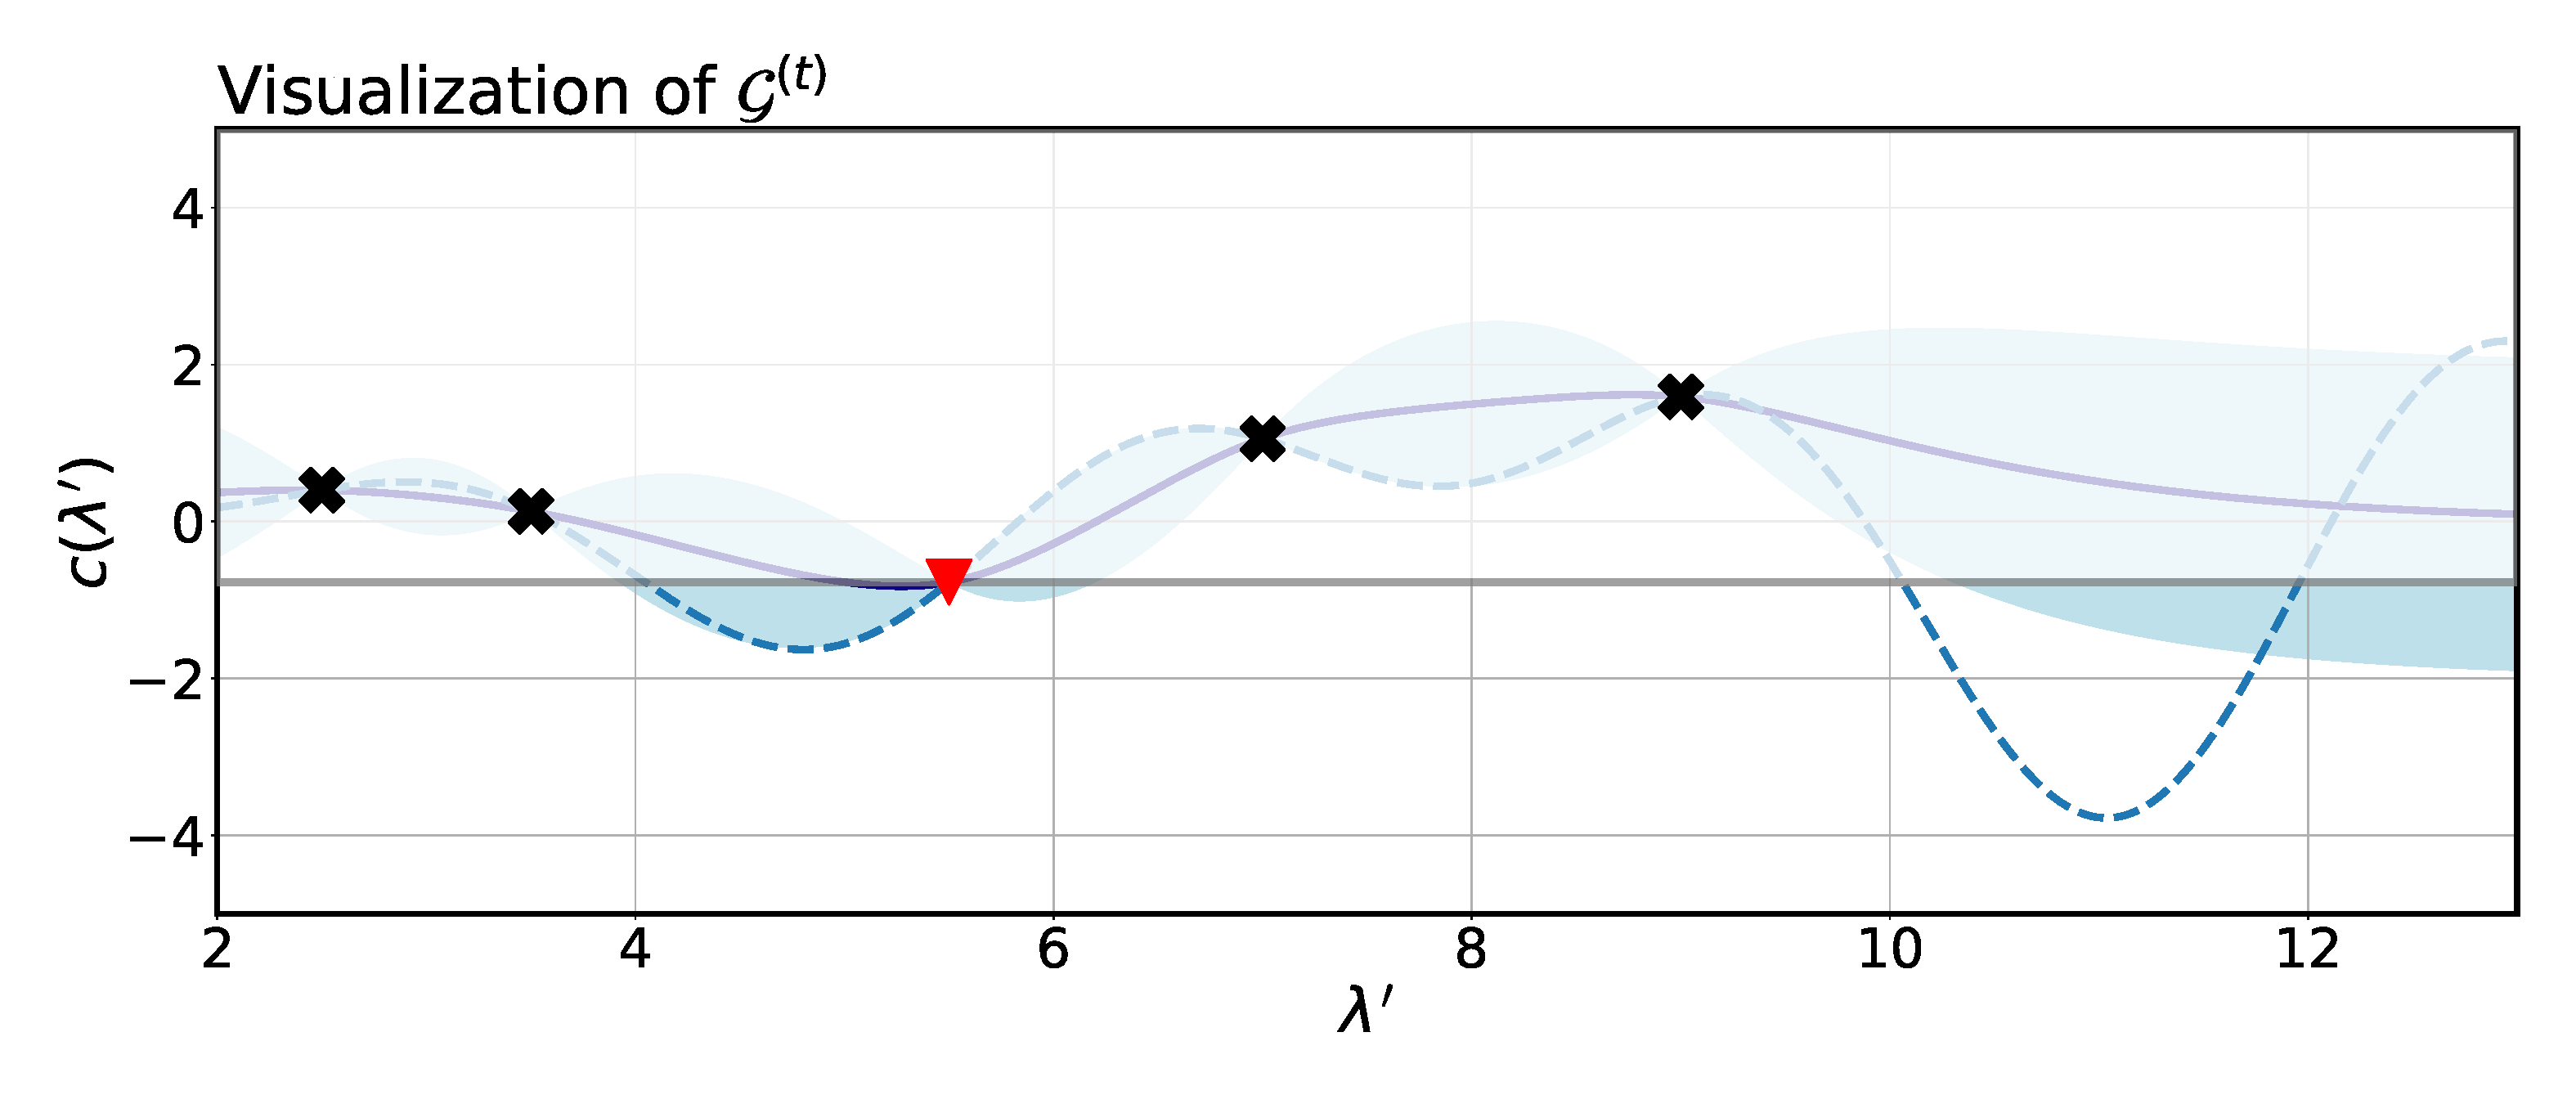
\includegraphics[width=\linewidth, height=0.7\textheight, keepaspectratio=true]{images/acq_func_images/pi/pi_3.pdf}};
        \node<.> [below=0.01\belowcaptionskip of img3, align=center]{Now let's drop the objective function - it's unknown after all!};
    
    
        \node<+> (img4) {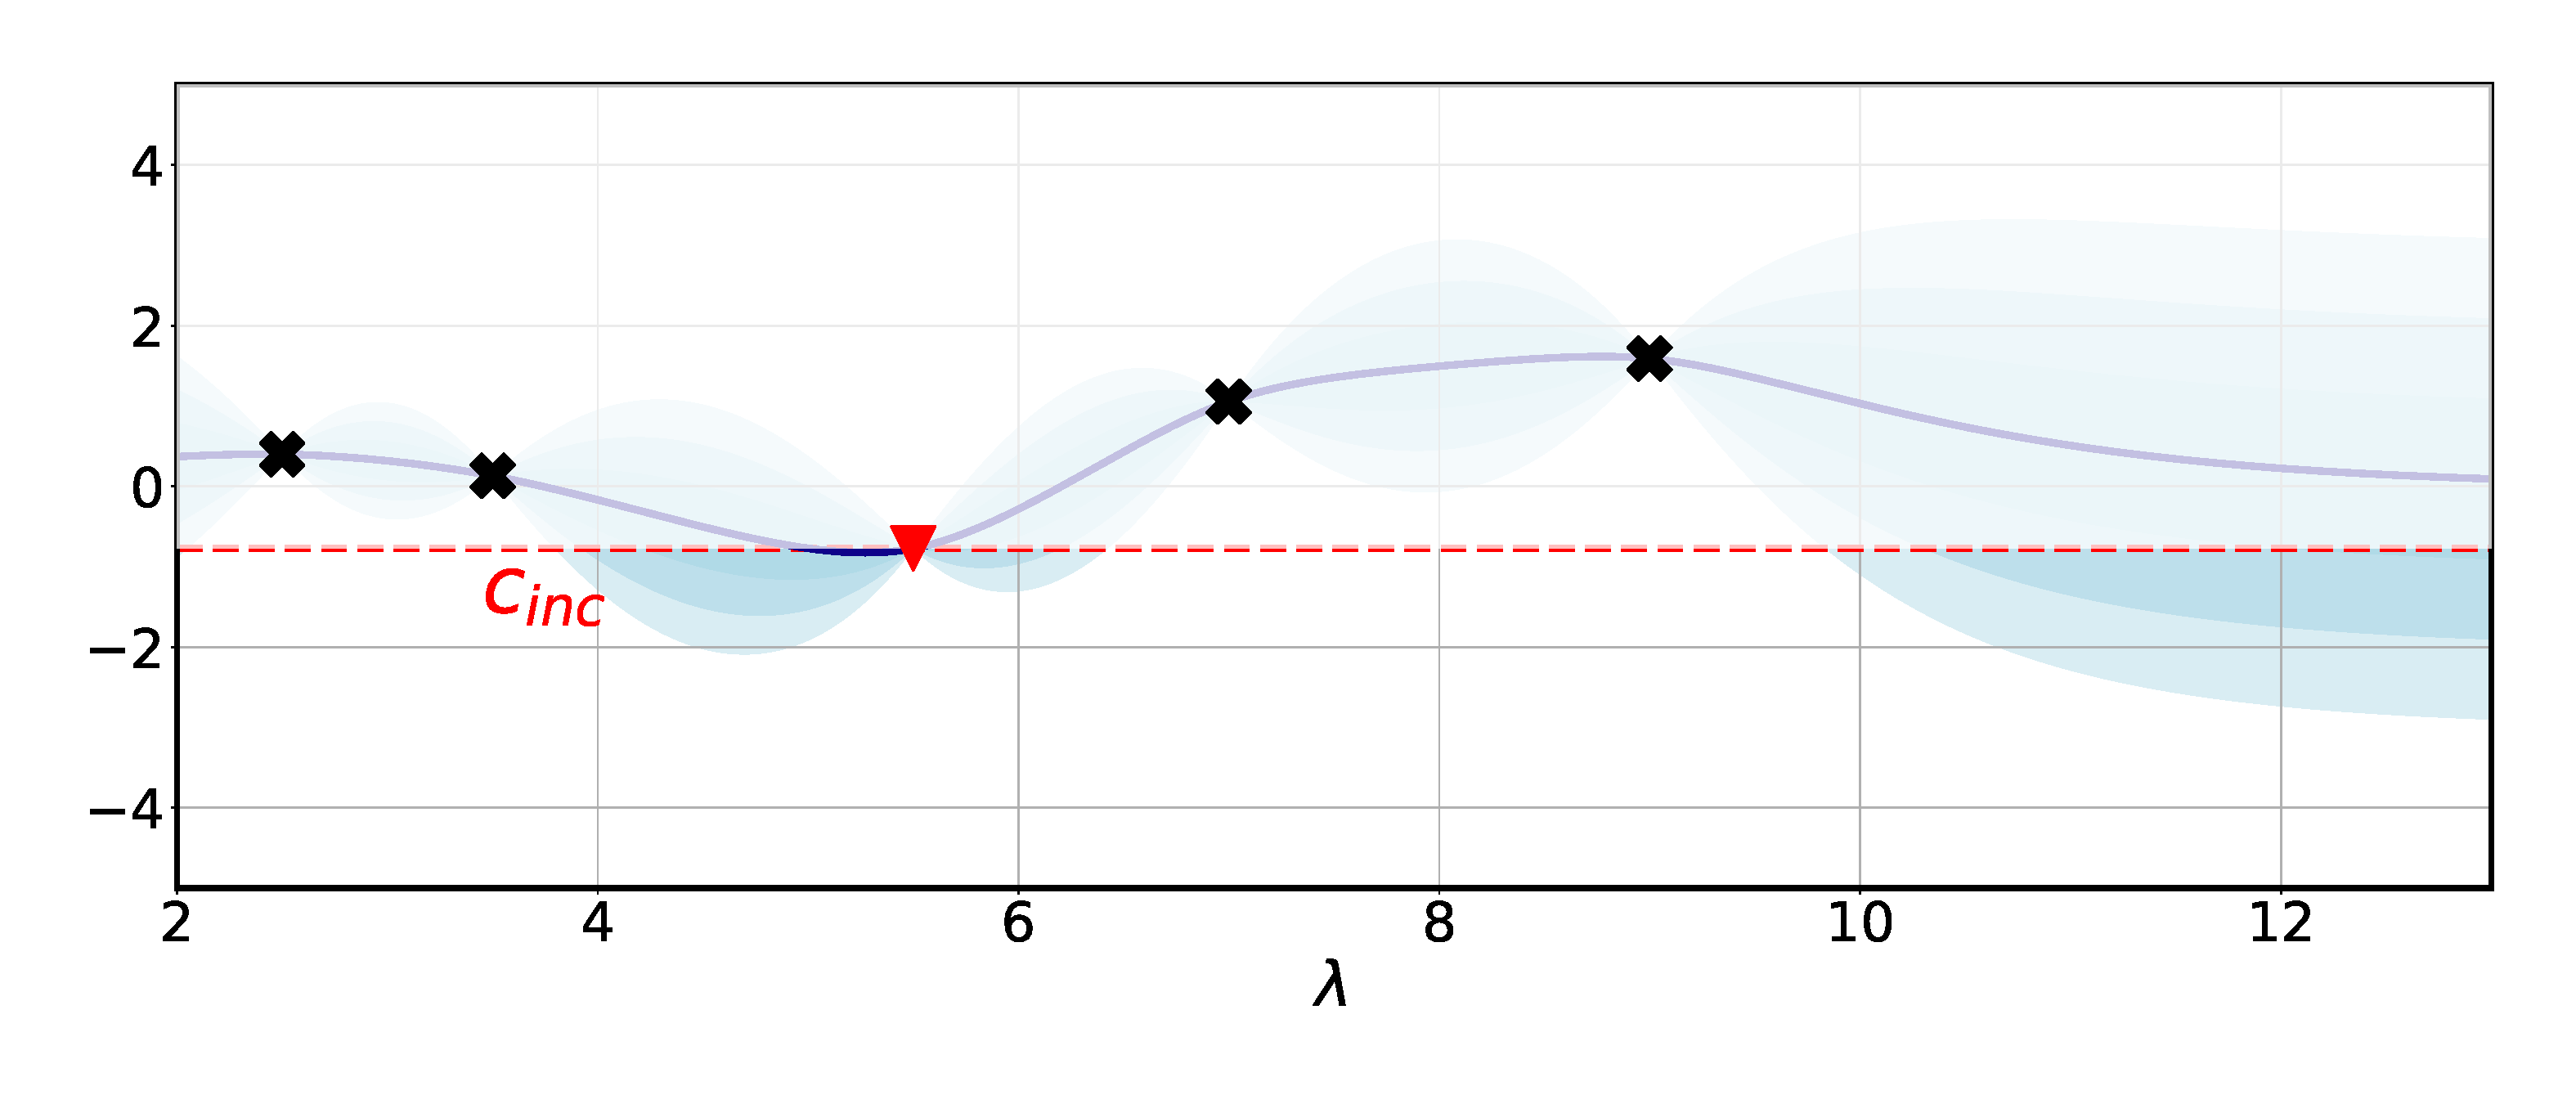
\includegraphics[width=\linewidth, height=0.7\textheight, keepaspectratio=true]{images/acq_func_images/pi/pi_4.pdf}};
        \node<.> [below=-1.0\belowcaptionskip of img4, align=center]{Intuitively, we care about the probability of improving over the current incumbent};
        \comment{We cannot be absolutely certain if there will be an improvement, but we are certain that if there is to be improvement, it is only possible in this zone.}
    
        \node<+> (img5) {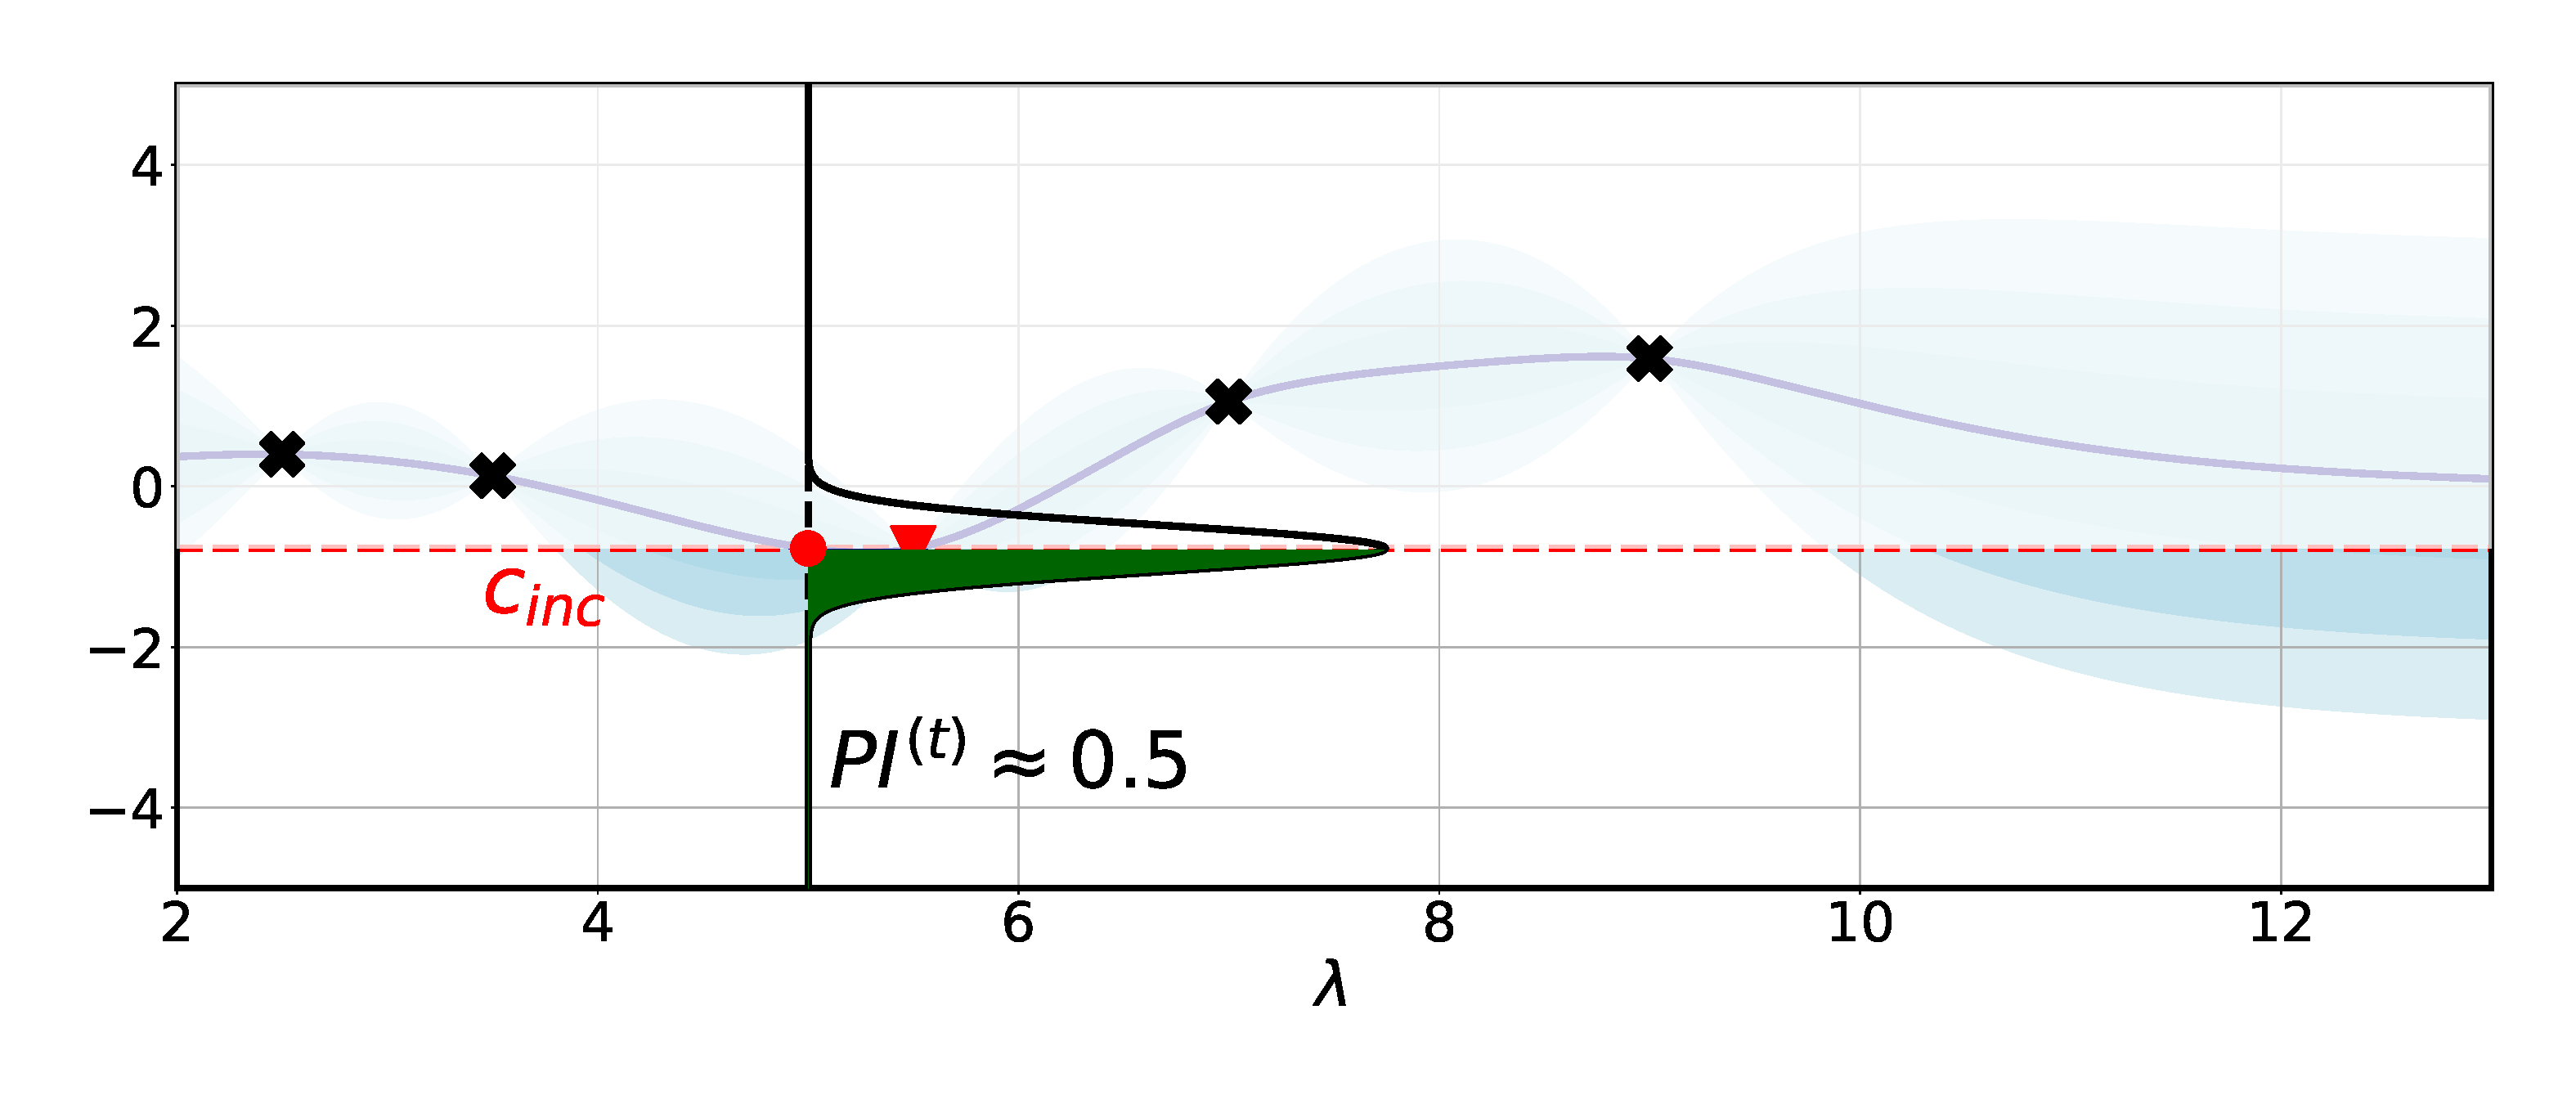
\includegraphics[width=\linewidth, height=0.7\textheight, keepaspectratio=true]{images/acq_func_images/pi/pi_5.pdf}};
        \node<.> [below=0.01\belowcaptionskip of img5, align=center]{PDF of a good candidate configuration. Only the green area is an improvement.};
    
        \node<+> (img6) {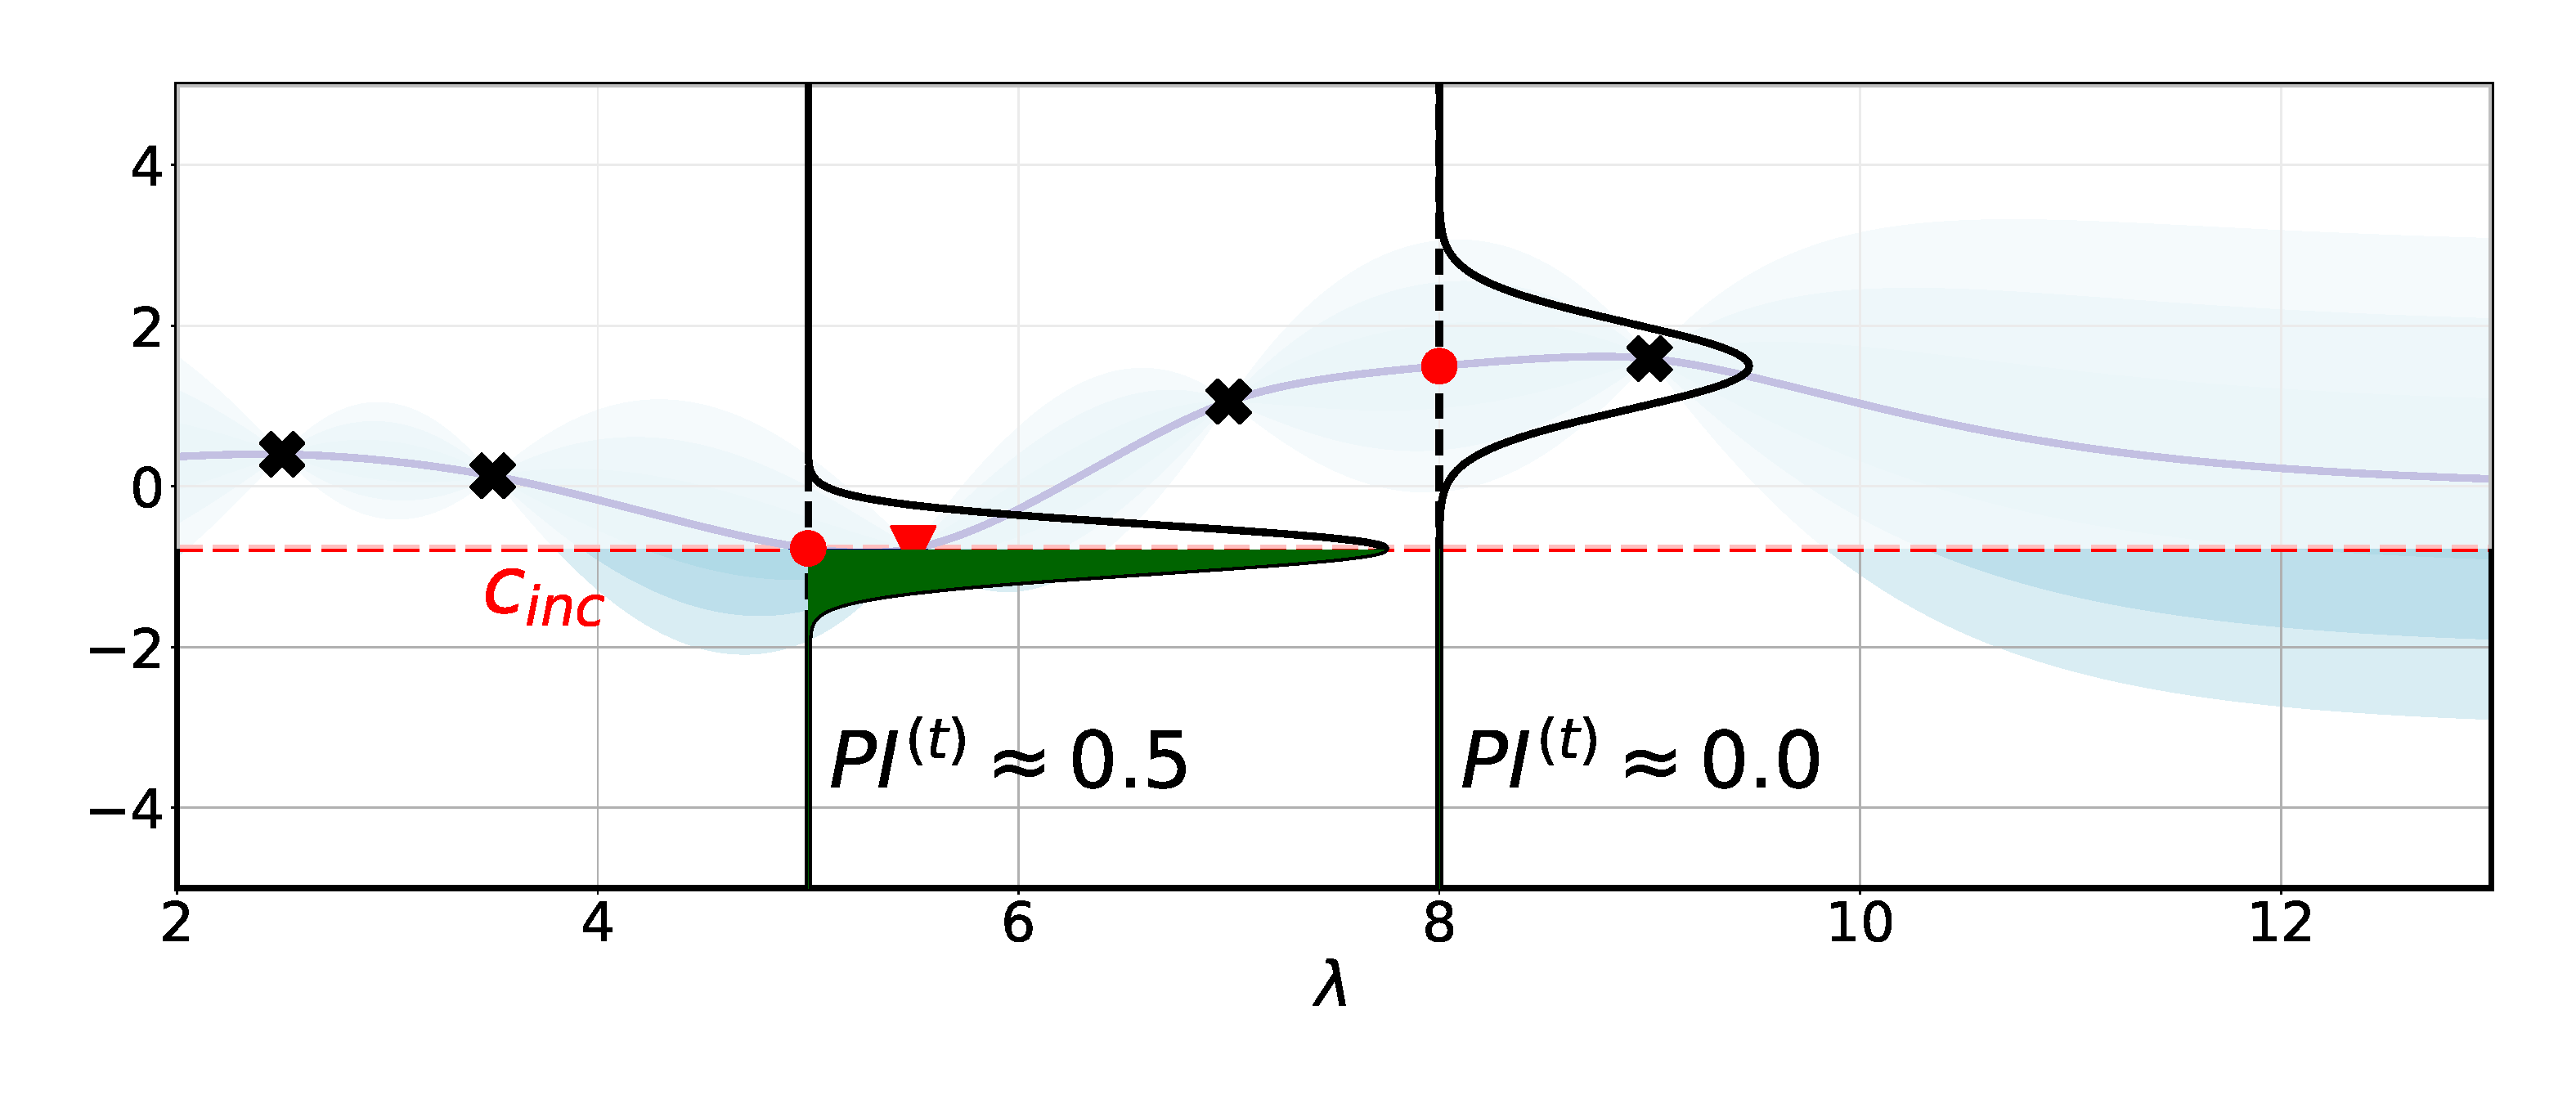
\includegraphics[width=\linewidth, height=0.7\textheight, keepaspectratio=true]{images/acq_func_images/pi/pi_6.pdf}};
        \node<.> [below=0.01\belowcaptionskip of img6, align=center]{PDF of a bad candidate configuration};
      \end{tikzpicture}
    % \end{figure}
    
}
\end{frame} 
% -----------------------------------------------------------------------
\begin{frame}[c]{Probability of Improvement (PI): Formal Definition}
%\framesubtitle{Probability of Improvement - Choosing a candidate}
%\comment{The definitions were adapted from the source to fit an acquisition function that is maximized and an objective function which is to be minimized.!}
\begin{itemize}
    \item We define the \alert{current incumbent at time step $t$} as: 
    $\incumbent[\bocount-1]\in\argmin_{\conf'\in\iter[\bocount-1]{\dataset}}\obs[\conf']$
    \item We write \alert{$\cost_{inc}$} shorthand for the \alert{cost of the current incumbent}: 
    $c_{inc} = \cost(\incumbent[\bocount-1])$
\smallskip
        \item The \alert{probability of improvement $\acq_{PI}(\conf)$} at a configuration $\conf$ is then defined as: 
        \alert{\[\iter{\acq}_{PI}(\conf) = P(\cost(\conf) \leq \cost_{inc}).\]}
    \vspace*{-0.5cm}
    \pause
    \item Since the predictive distribution for $\cost(\conf)$ is a Gaussian $\normaldist(\iter[\bocount-1]{\mean}(\conf), \iter[\bocount-1]{\variance}(\conf))$, this can be written as:
    \[
        \alert{\iter{\acq}_{PI}(\conf) = \cdf[Z]}, \quad \text{with } Z = \dfrac{\cost_{inc} - \iter[\bocount-1]{\mean}(\conf) - \xi}{\iter[\bocount-1]{\stddev}(\conf)}, 
    \]
    \newline
    where $\cdf(\cdot)$ is the CDF of the standard normal distribution and $\xi$ is an optional exploration parameter
    \pause
    \item[] \[\boxed{\text{Choose}\;\;\bonextsample \in \argmax_{\conf\in\pcs}(\iter{\acq}_{PI}(\conf))}\]
%    \comment{Source: Tutorial by Brochu et al.: https://arxiv.org/pdf/1012.2599.pdf }
\end{itemize}
\end{frame}
%-----------------------------------------------------------------------
\begin{frame}[t]{Expected Improvement (EI): Concept}
%\framesubtitle{Expected Improvement - Concept}

% \begin{figure}
  \centering
  \begin{tikzpicture}
    \node<+> (img1) {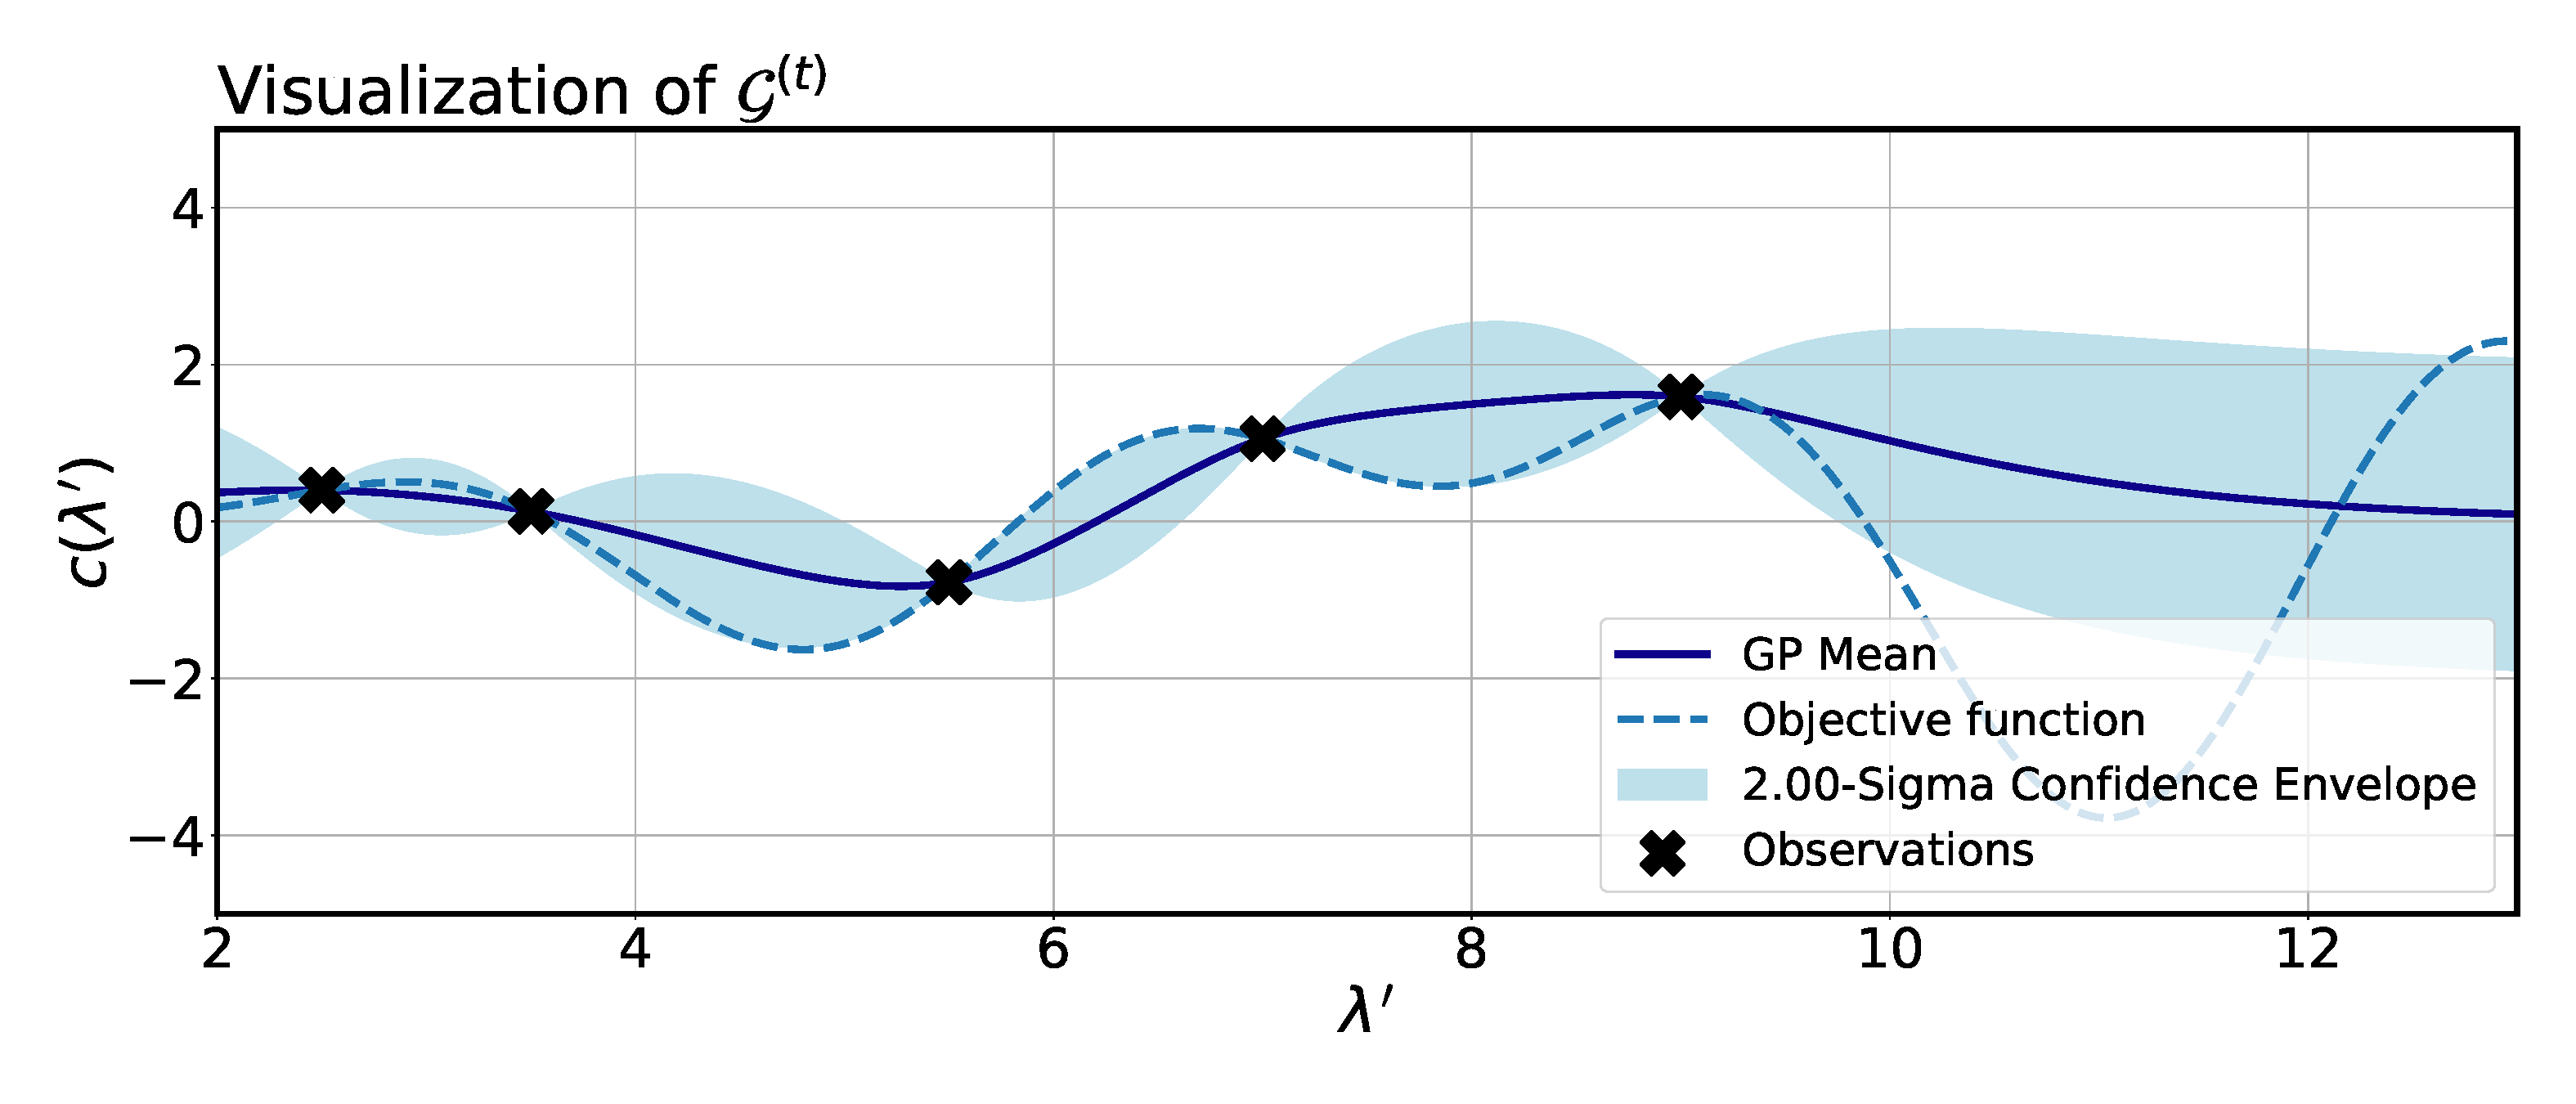
\includegraphics[width=\linewidth, height=0.7\textheight, keepaspectratio=true]{images/acq_func_images/ei/ei_1.pdf}};
    \node<.> [below=0.01\belowcaptionskip of img1, align=center]{Given the surrogate fit at iteration $\bocount$};

    \node<+> (img2a) {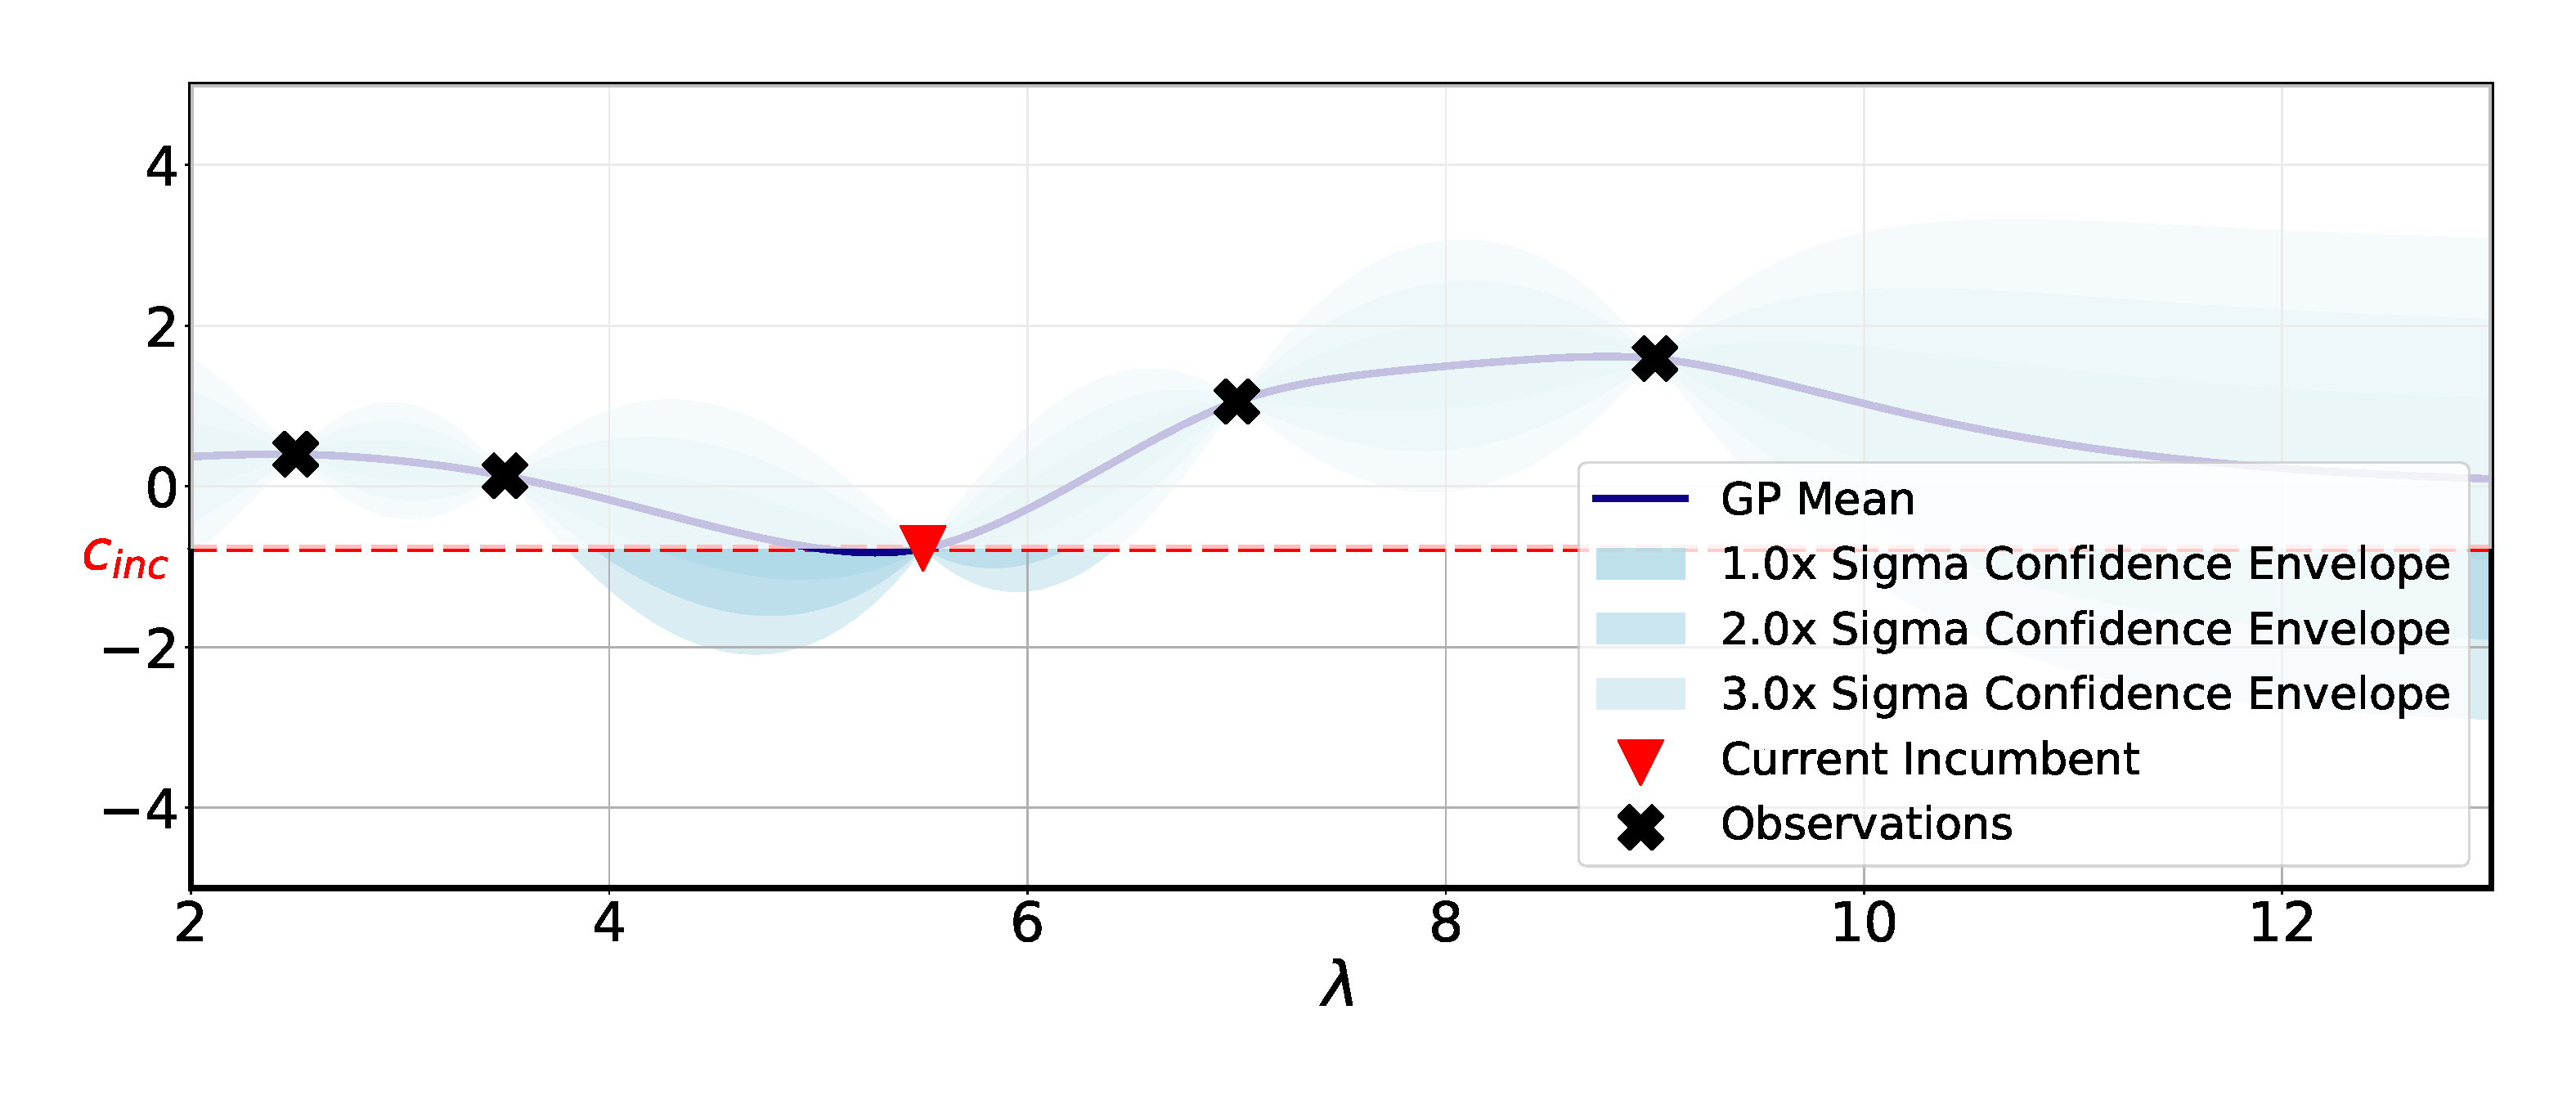
\includegraphics[width=\linewidth, height=0.7\textheight, keepaspectratio=true]{images/acq_func_images/ei/ei_2a.pdf}};
    \node<.> [below=0.01\belowcaptionskip of img2a, align=center]{Region of probable improvement -- but \alert{how large} is the improvement?};

    \node<+> (img2b) {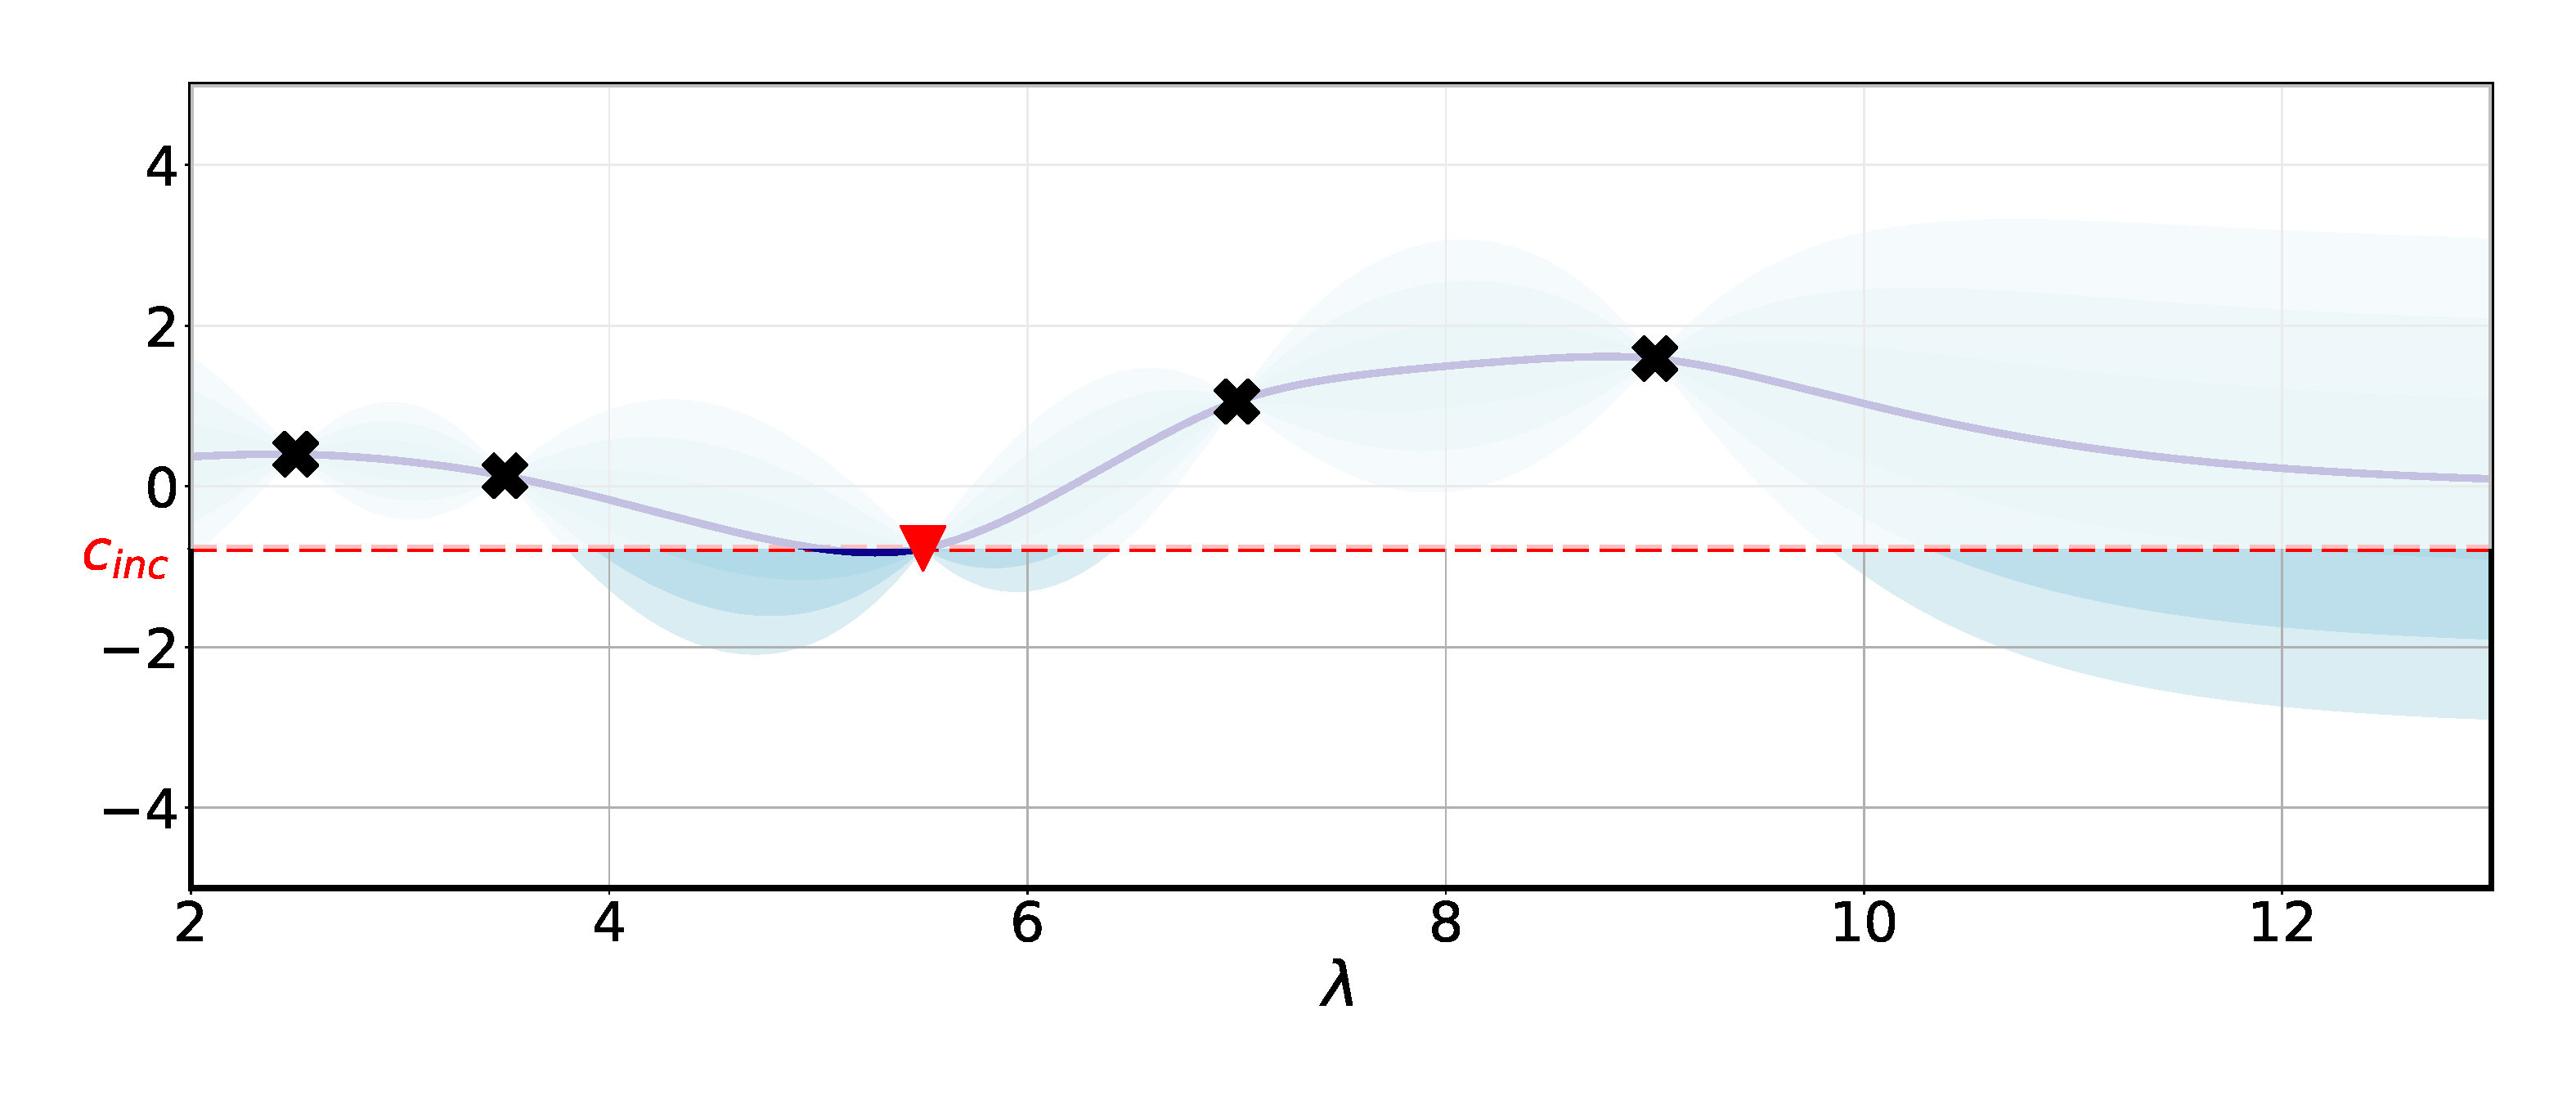
\includegraphics[width=\linewidth, height=0.7\textheight, keepaspectratio=true]{images/acq_func_images/ei/ei_2b.pdf}};
    \node<.> [below=0.01\belowcaptionskip of img2b, align=center]{Region of probable improvement -- but \alert{how large} is the improvement?};

    \node<+> (img3) {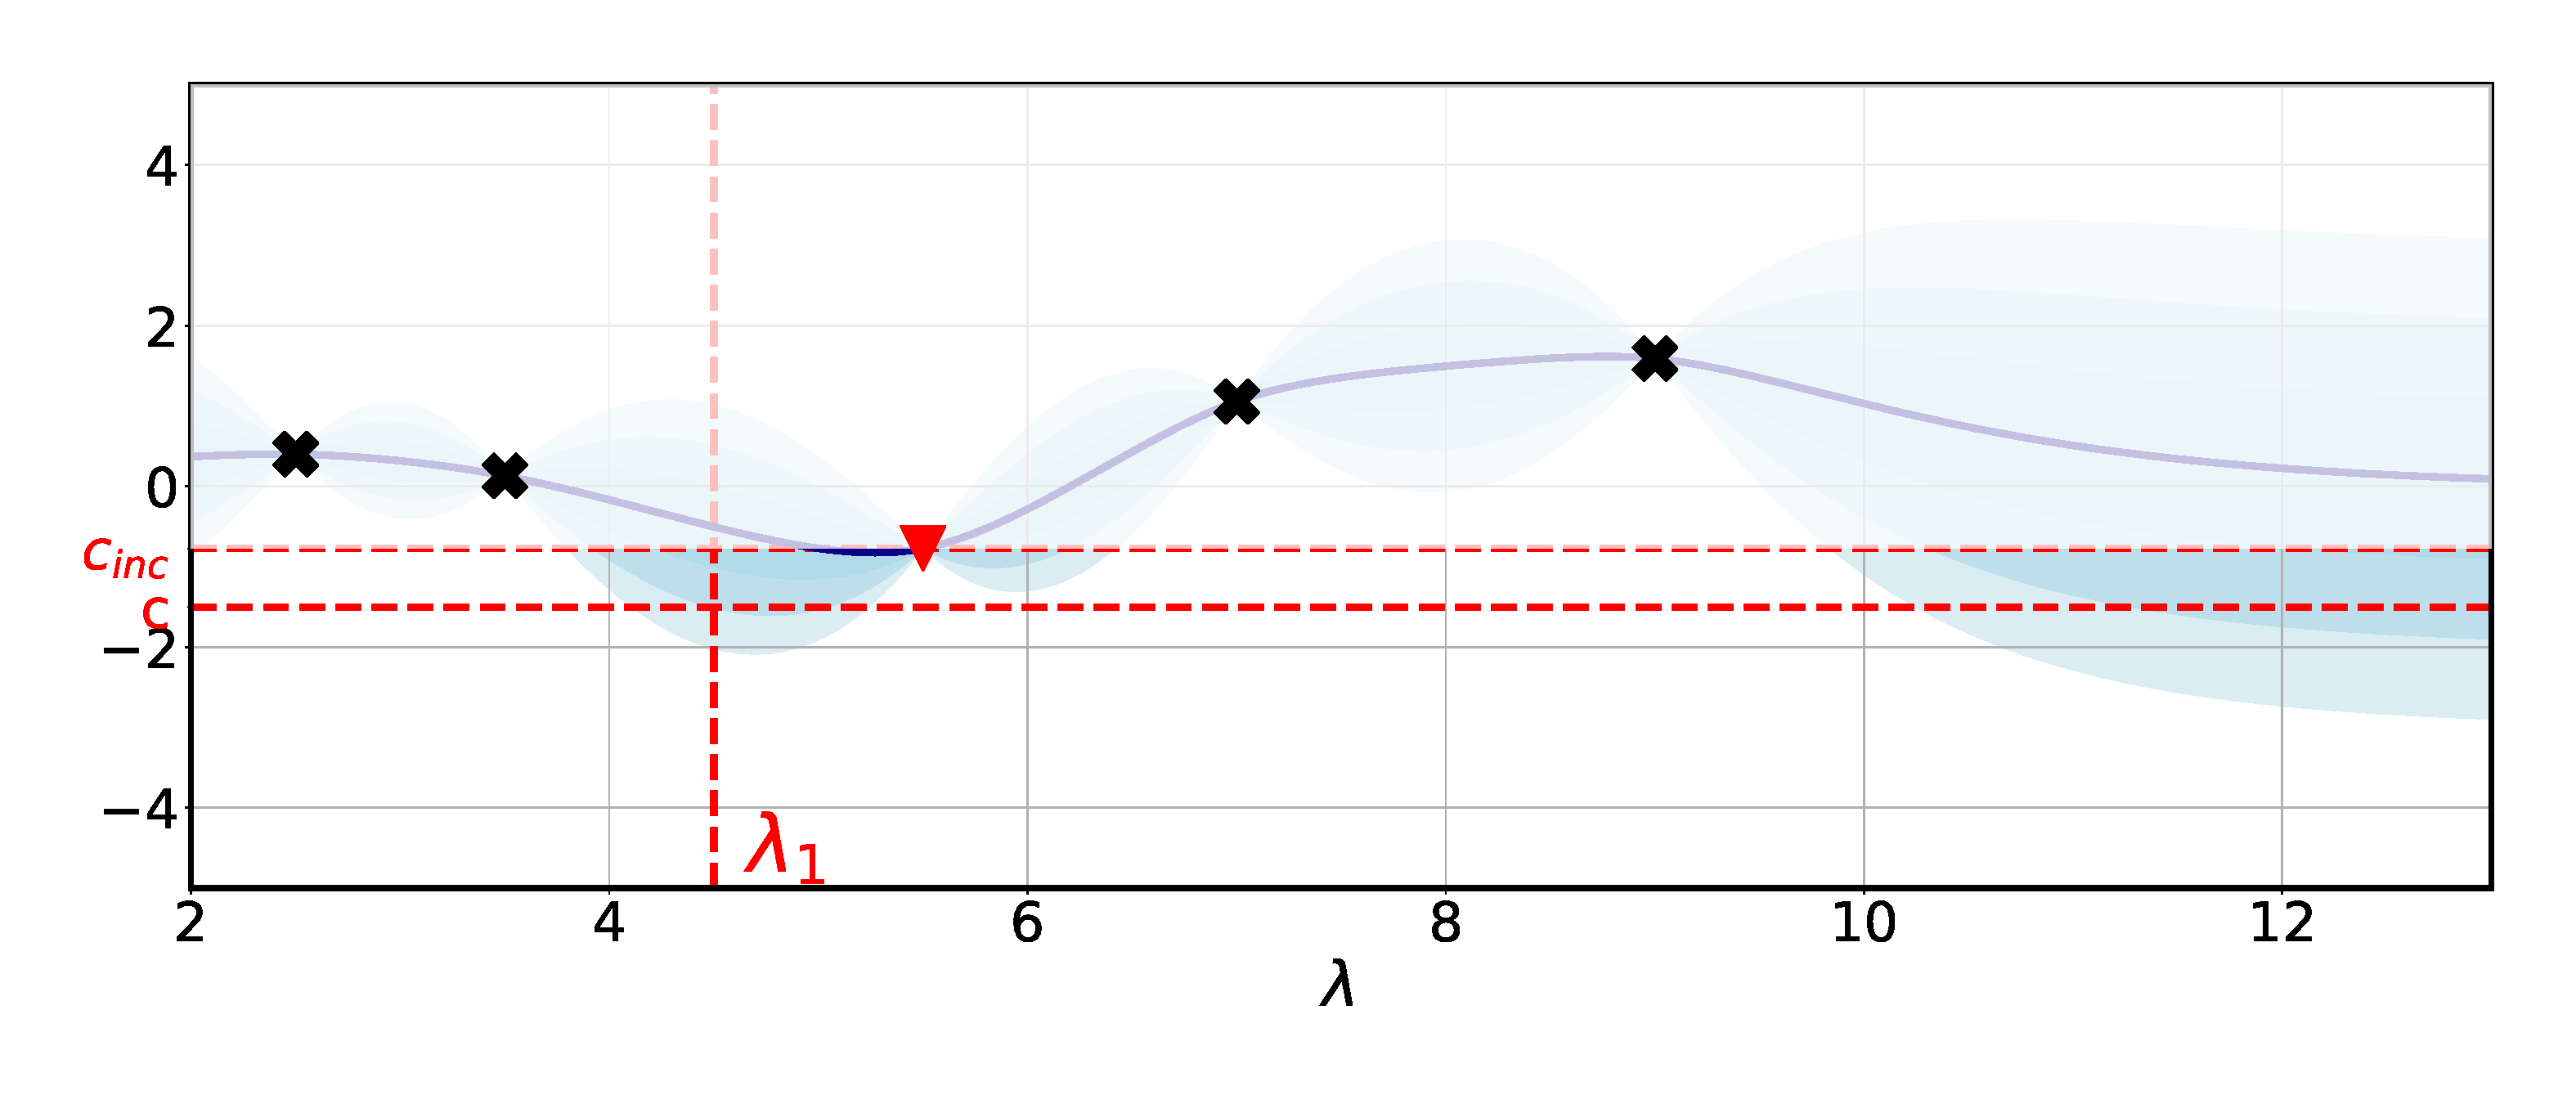
\includegraphics[width=\linewidth, height=0.7\textheight, keepaspectratio=true]{images/acq_func_images/ei/ei_3.pdf}};
    \node<.> [below=0.01\belowcaptionskip of img3, align=center]{Hypothetical \emph{real} cost $c$ at a given $\conf$ - unknown in practice without evaluating};

    \node<+> (img4) {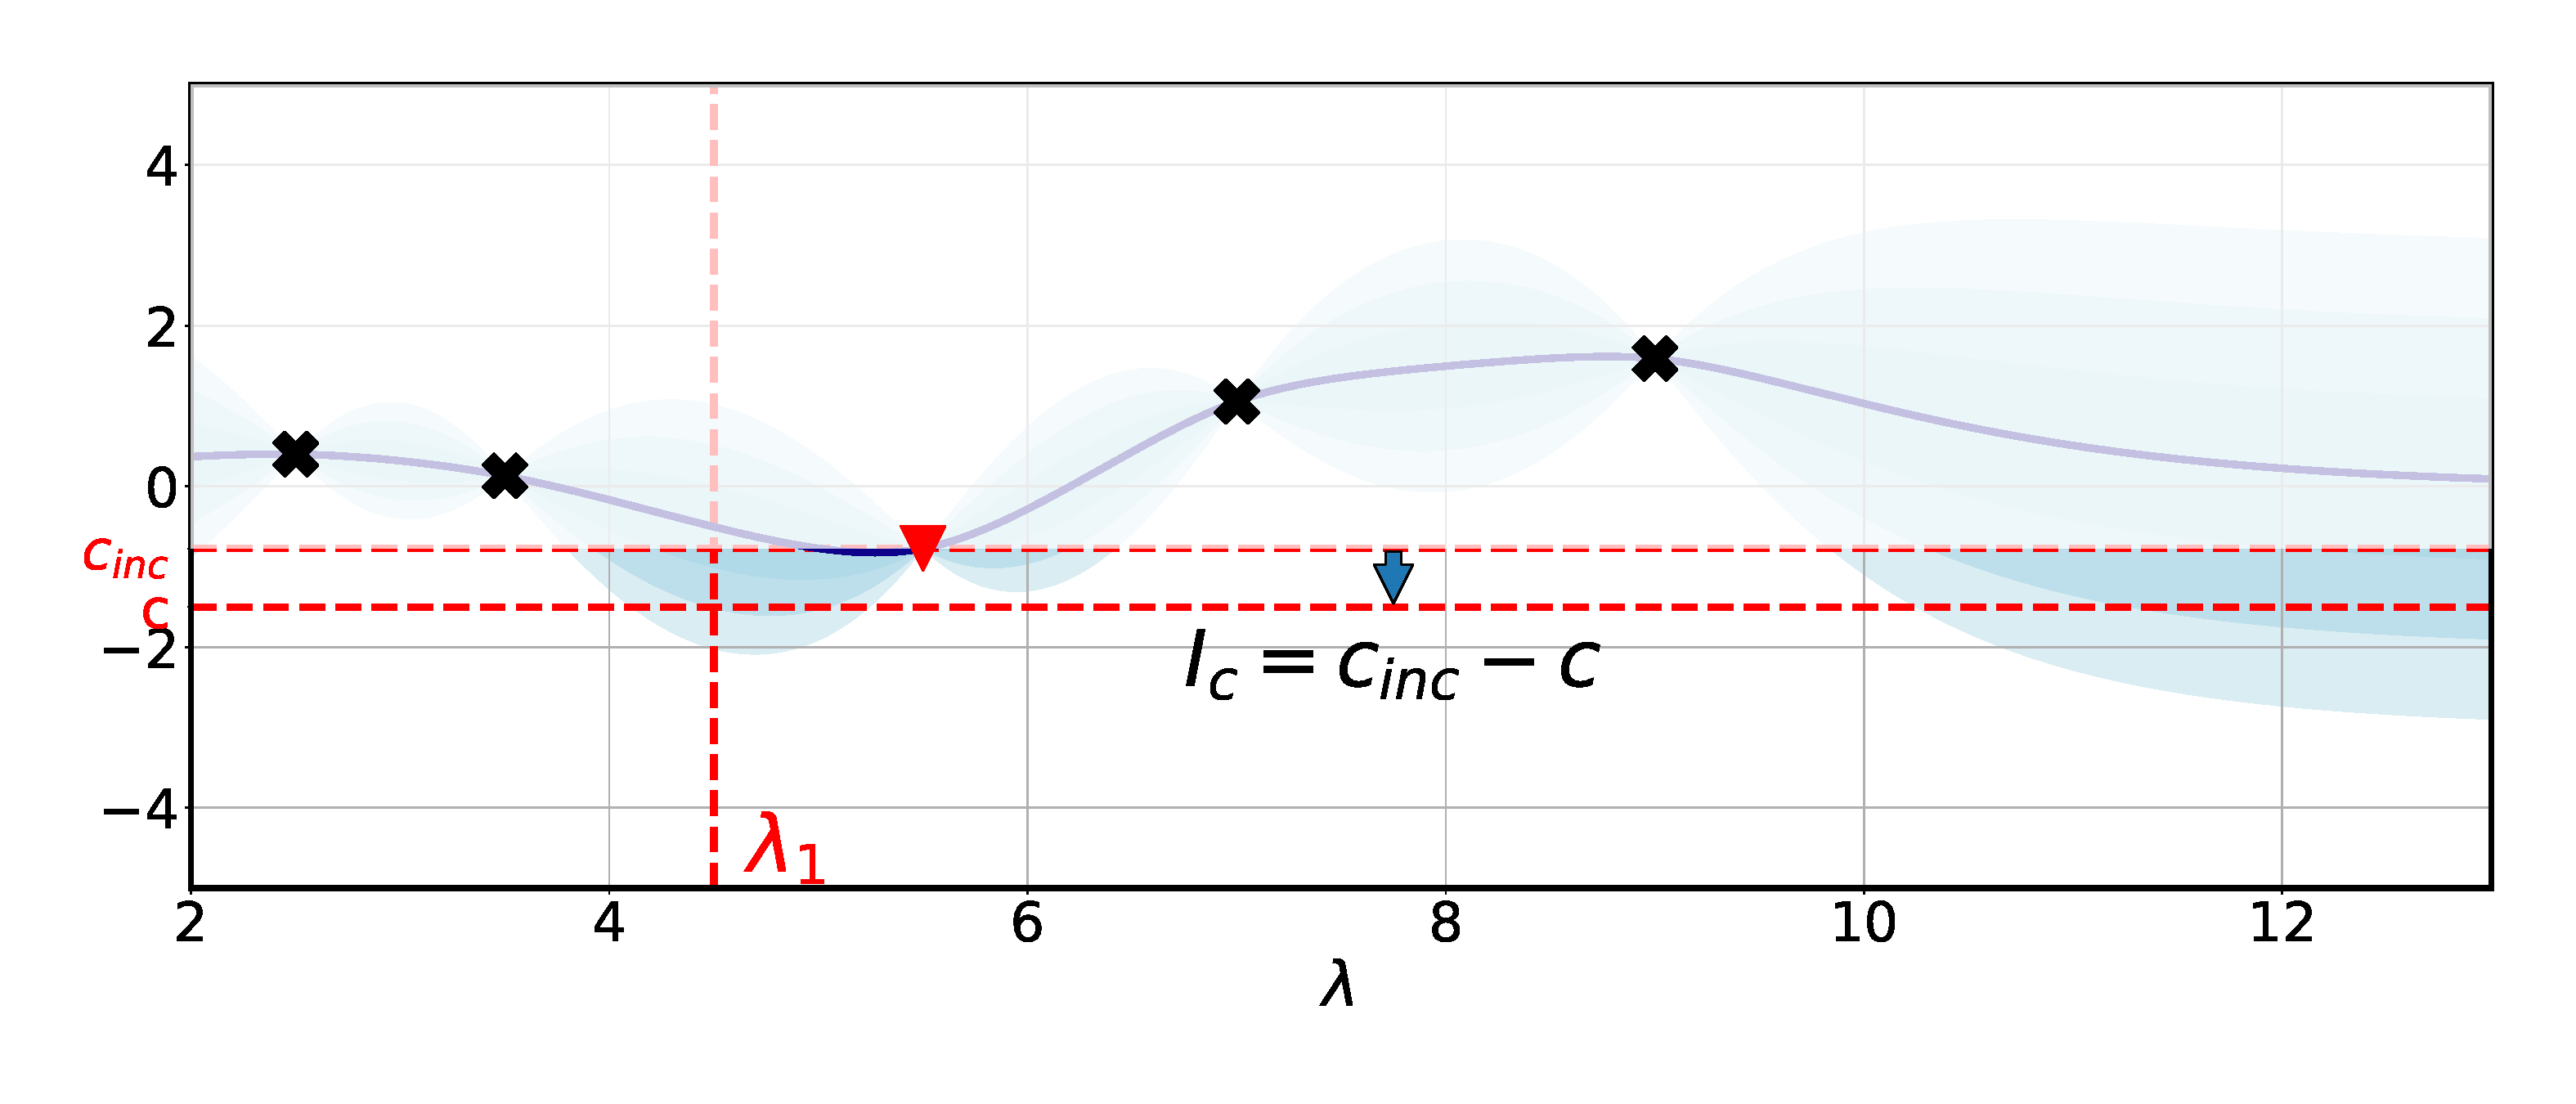
\includegraphics[width=\linewidth, height=0.7\textheight, keepaspectratio=true]{images/acq_func_images/ei/ei_4.pdf}};
    \node<.> [below=-0.01\belowcaptionskip of img4, align=center]{Given a hypothetical $c$, we can compute the improvement $I_c(\conf)$};
%    Without performing an actual evaluation, we cannot calculate $\iter{I}(\conf)$};

    \node<+> (img5) {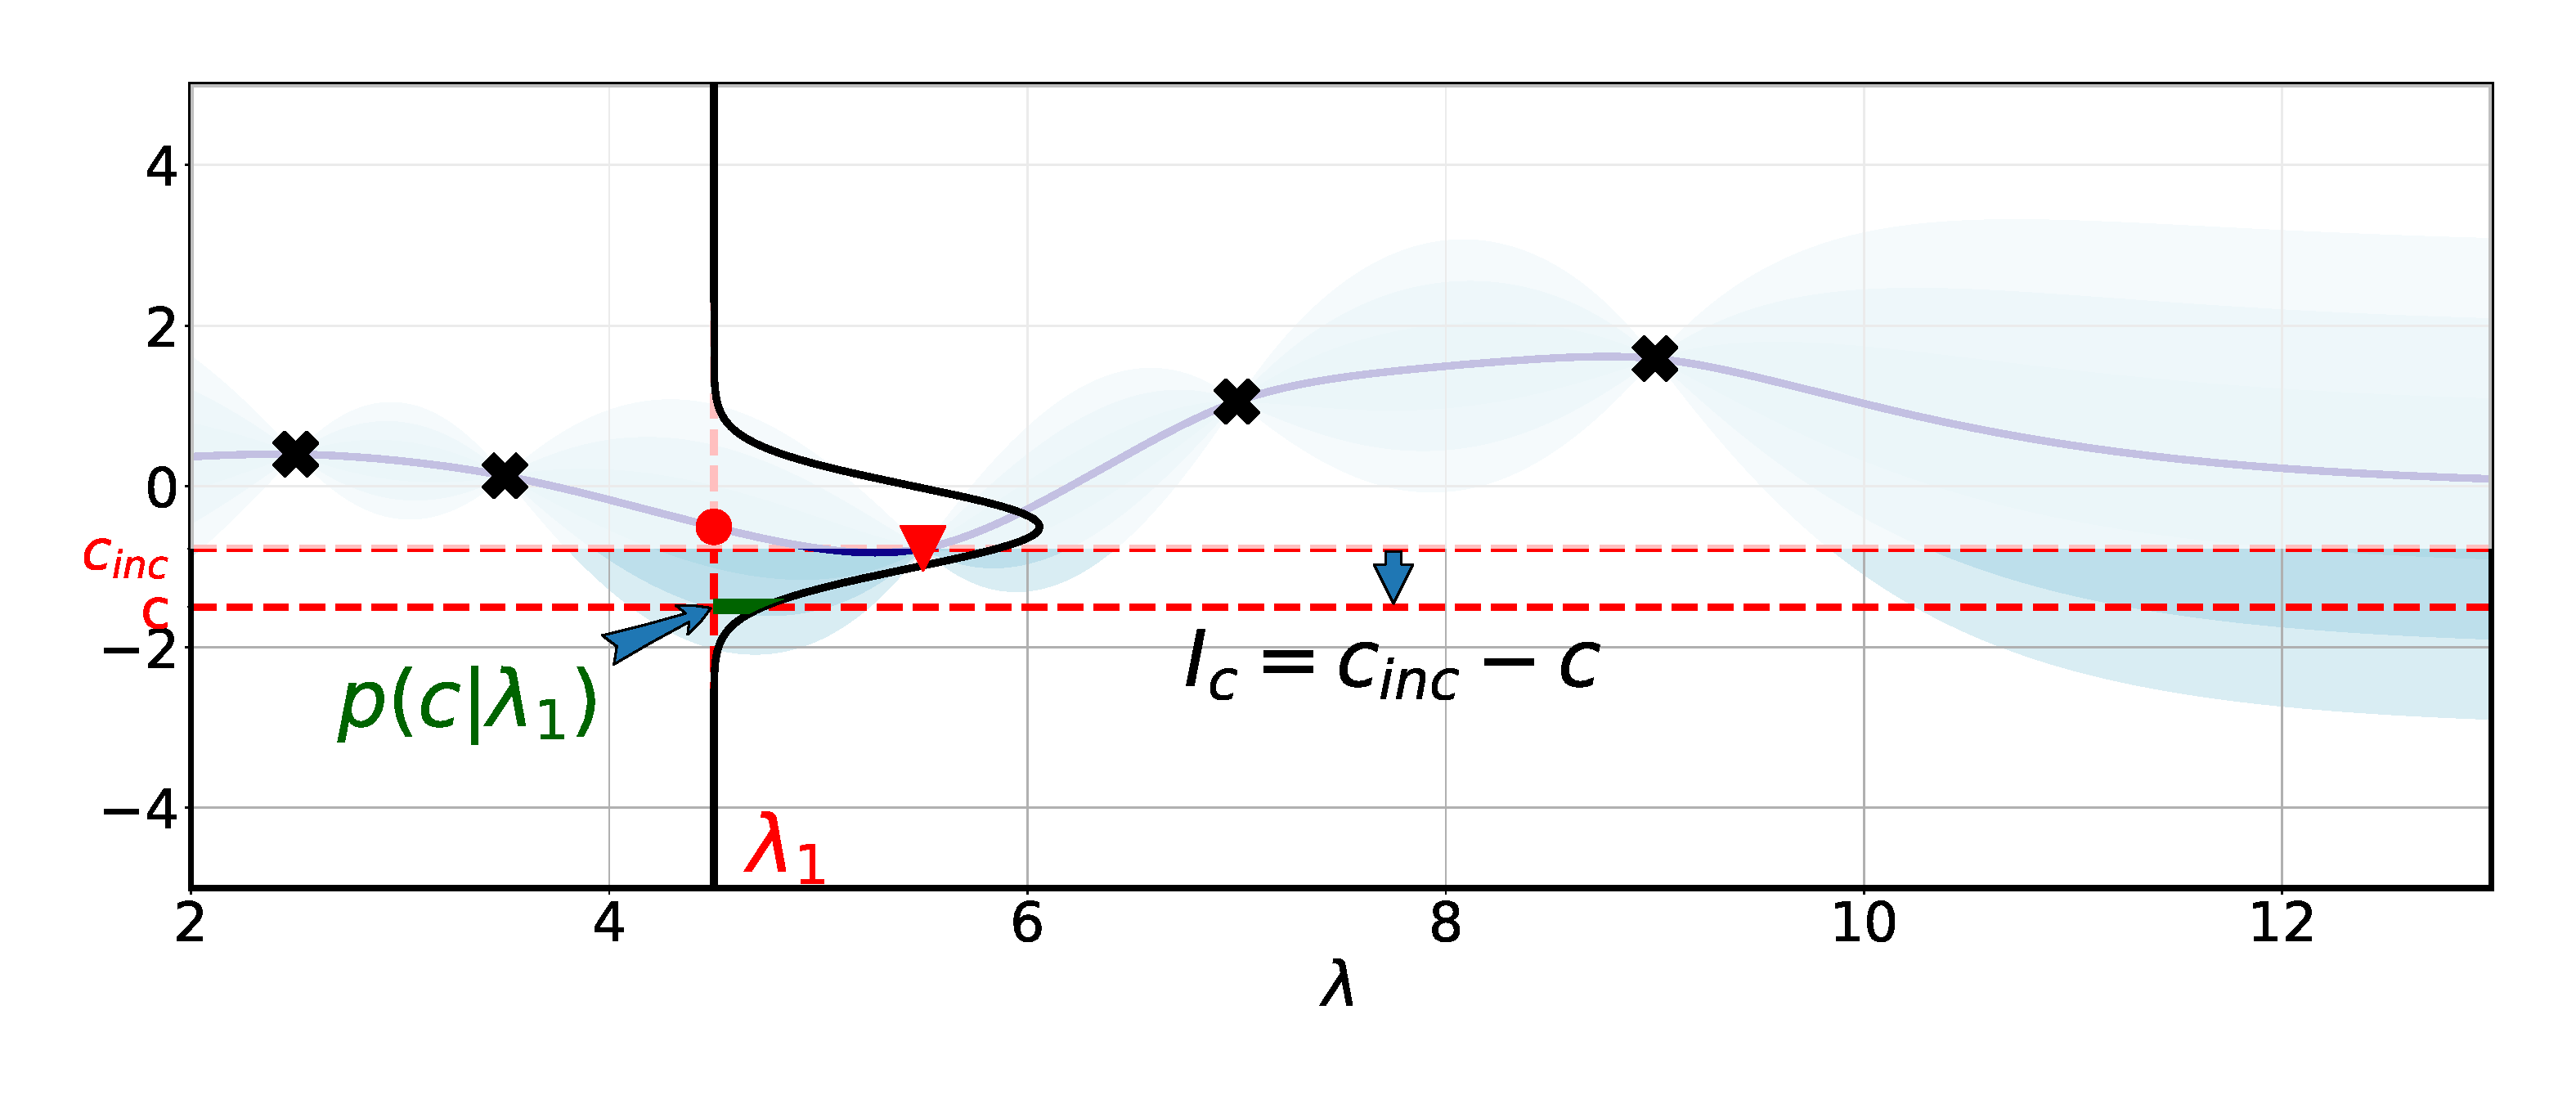
\includegraphics[width=\linewidth, height=0.7\textheight, keepaspectratio=true]{images/acq_func_images/ei/ei_5.pdf}};
    \node<.> [below=0.01\belowcaptionskip of img5, align=center]{Given $\surro(\conf) = \normaldist( \mean(\conf), \variance(\conf))$, we can also compute $p(\cost|\conf)$.};

    \node<+> (img6) {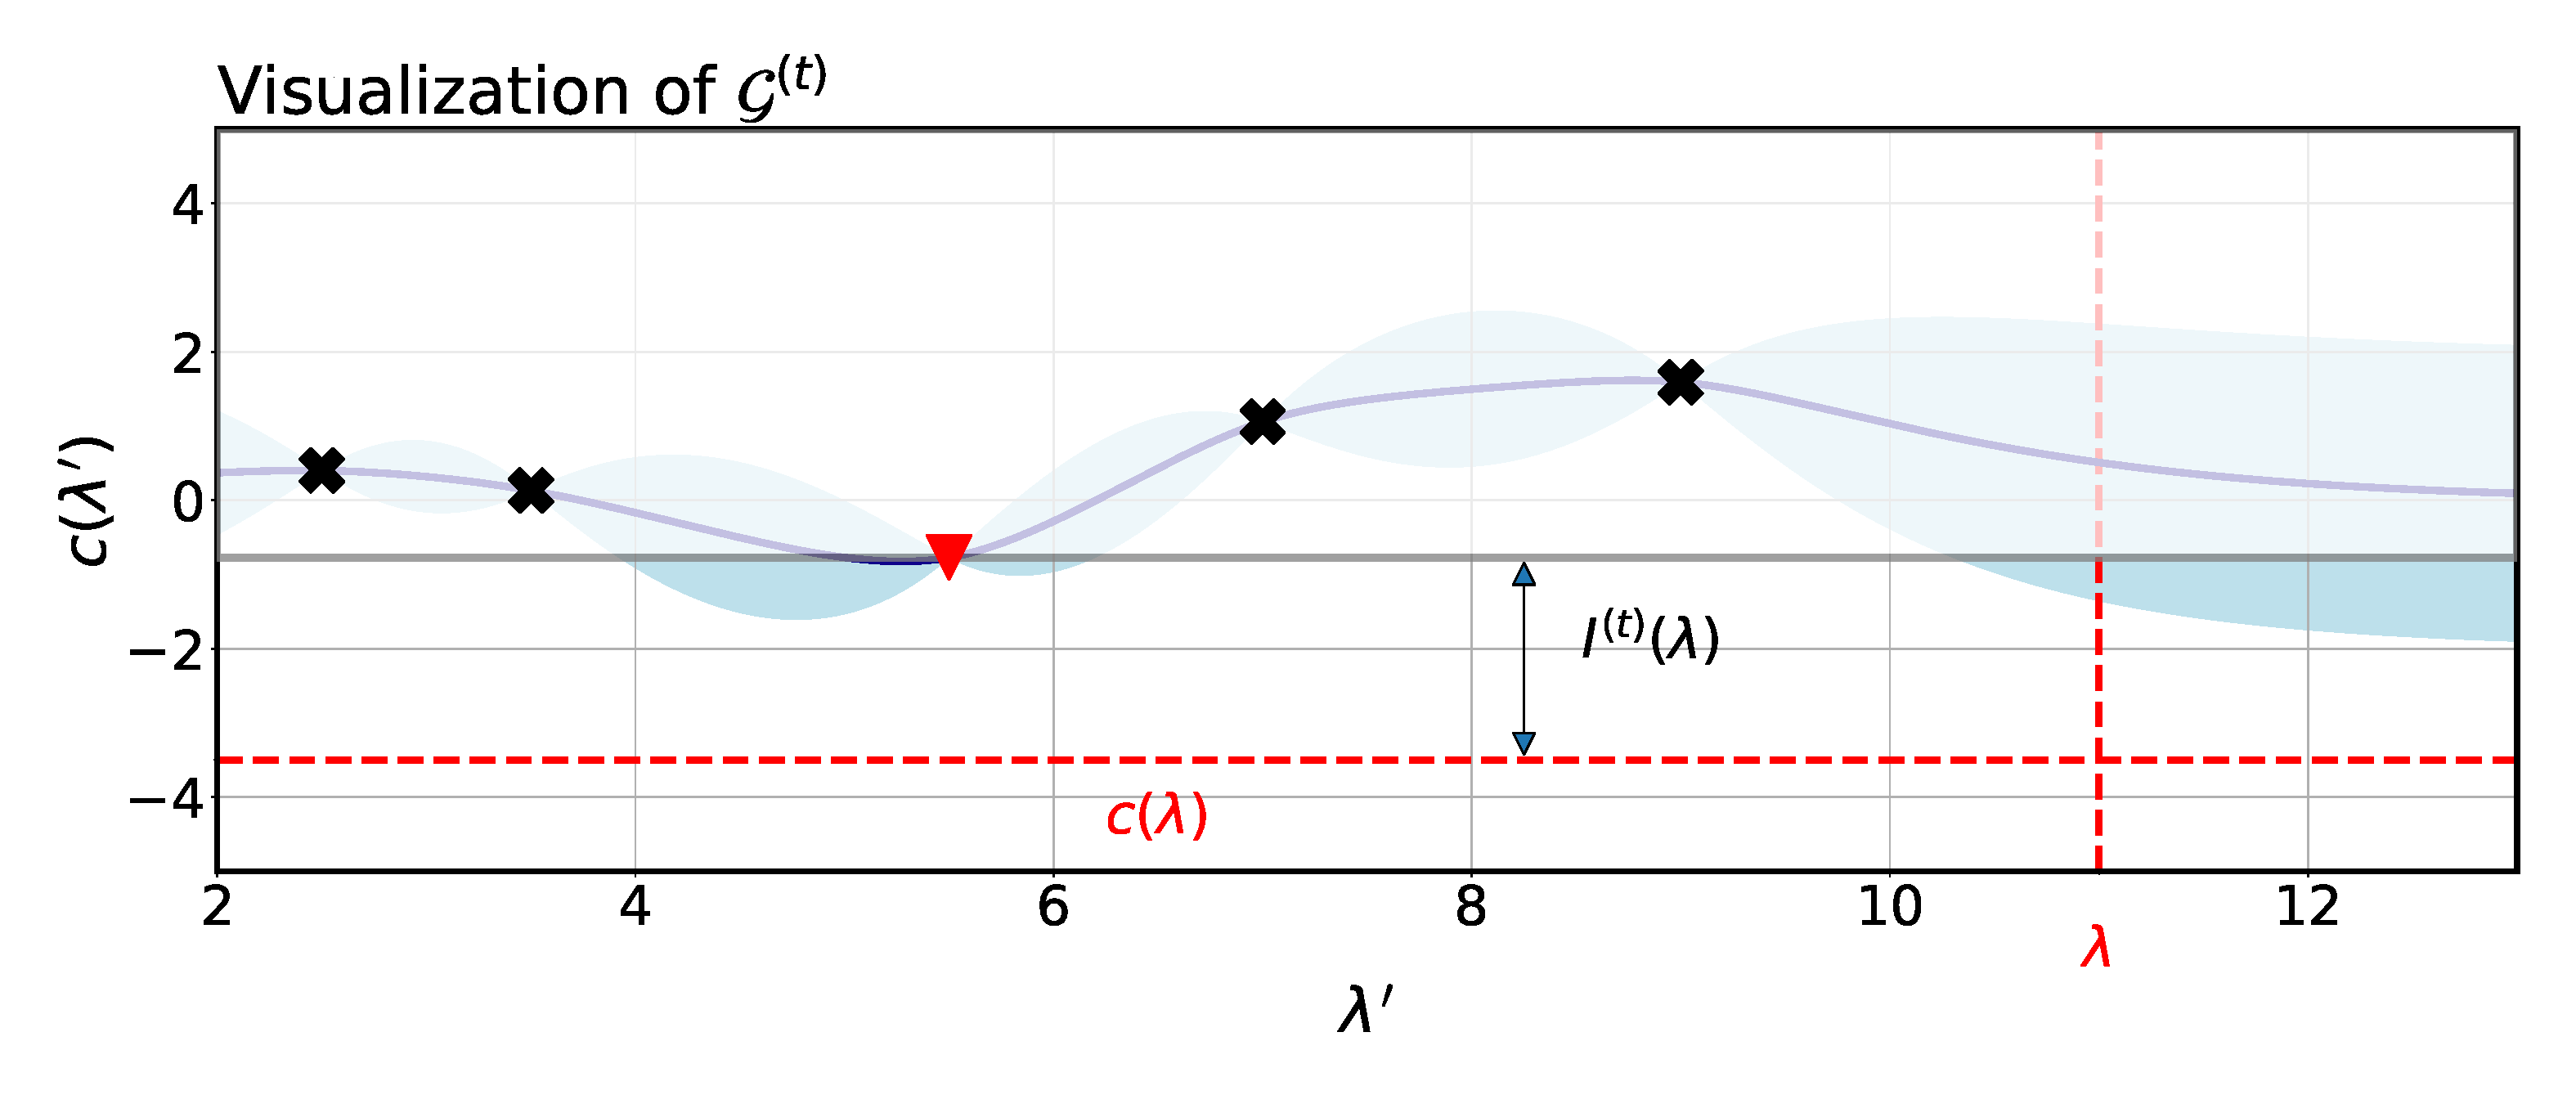
\includegraphics[width=\linewidth, height=0.7\textheight, keepaspectratio=true]{images/acq_func_images/ei/ei_6.pdf}};
    \node<.> [below=-0.01\belowcaptionskip of img6, align=center]{Compare the likelihood of a given improvement for two different configurations $\conf_1$ and $\conf_2$};

    \node<+> (img7) {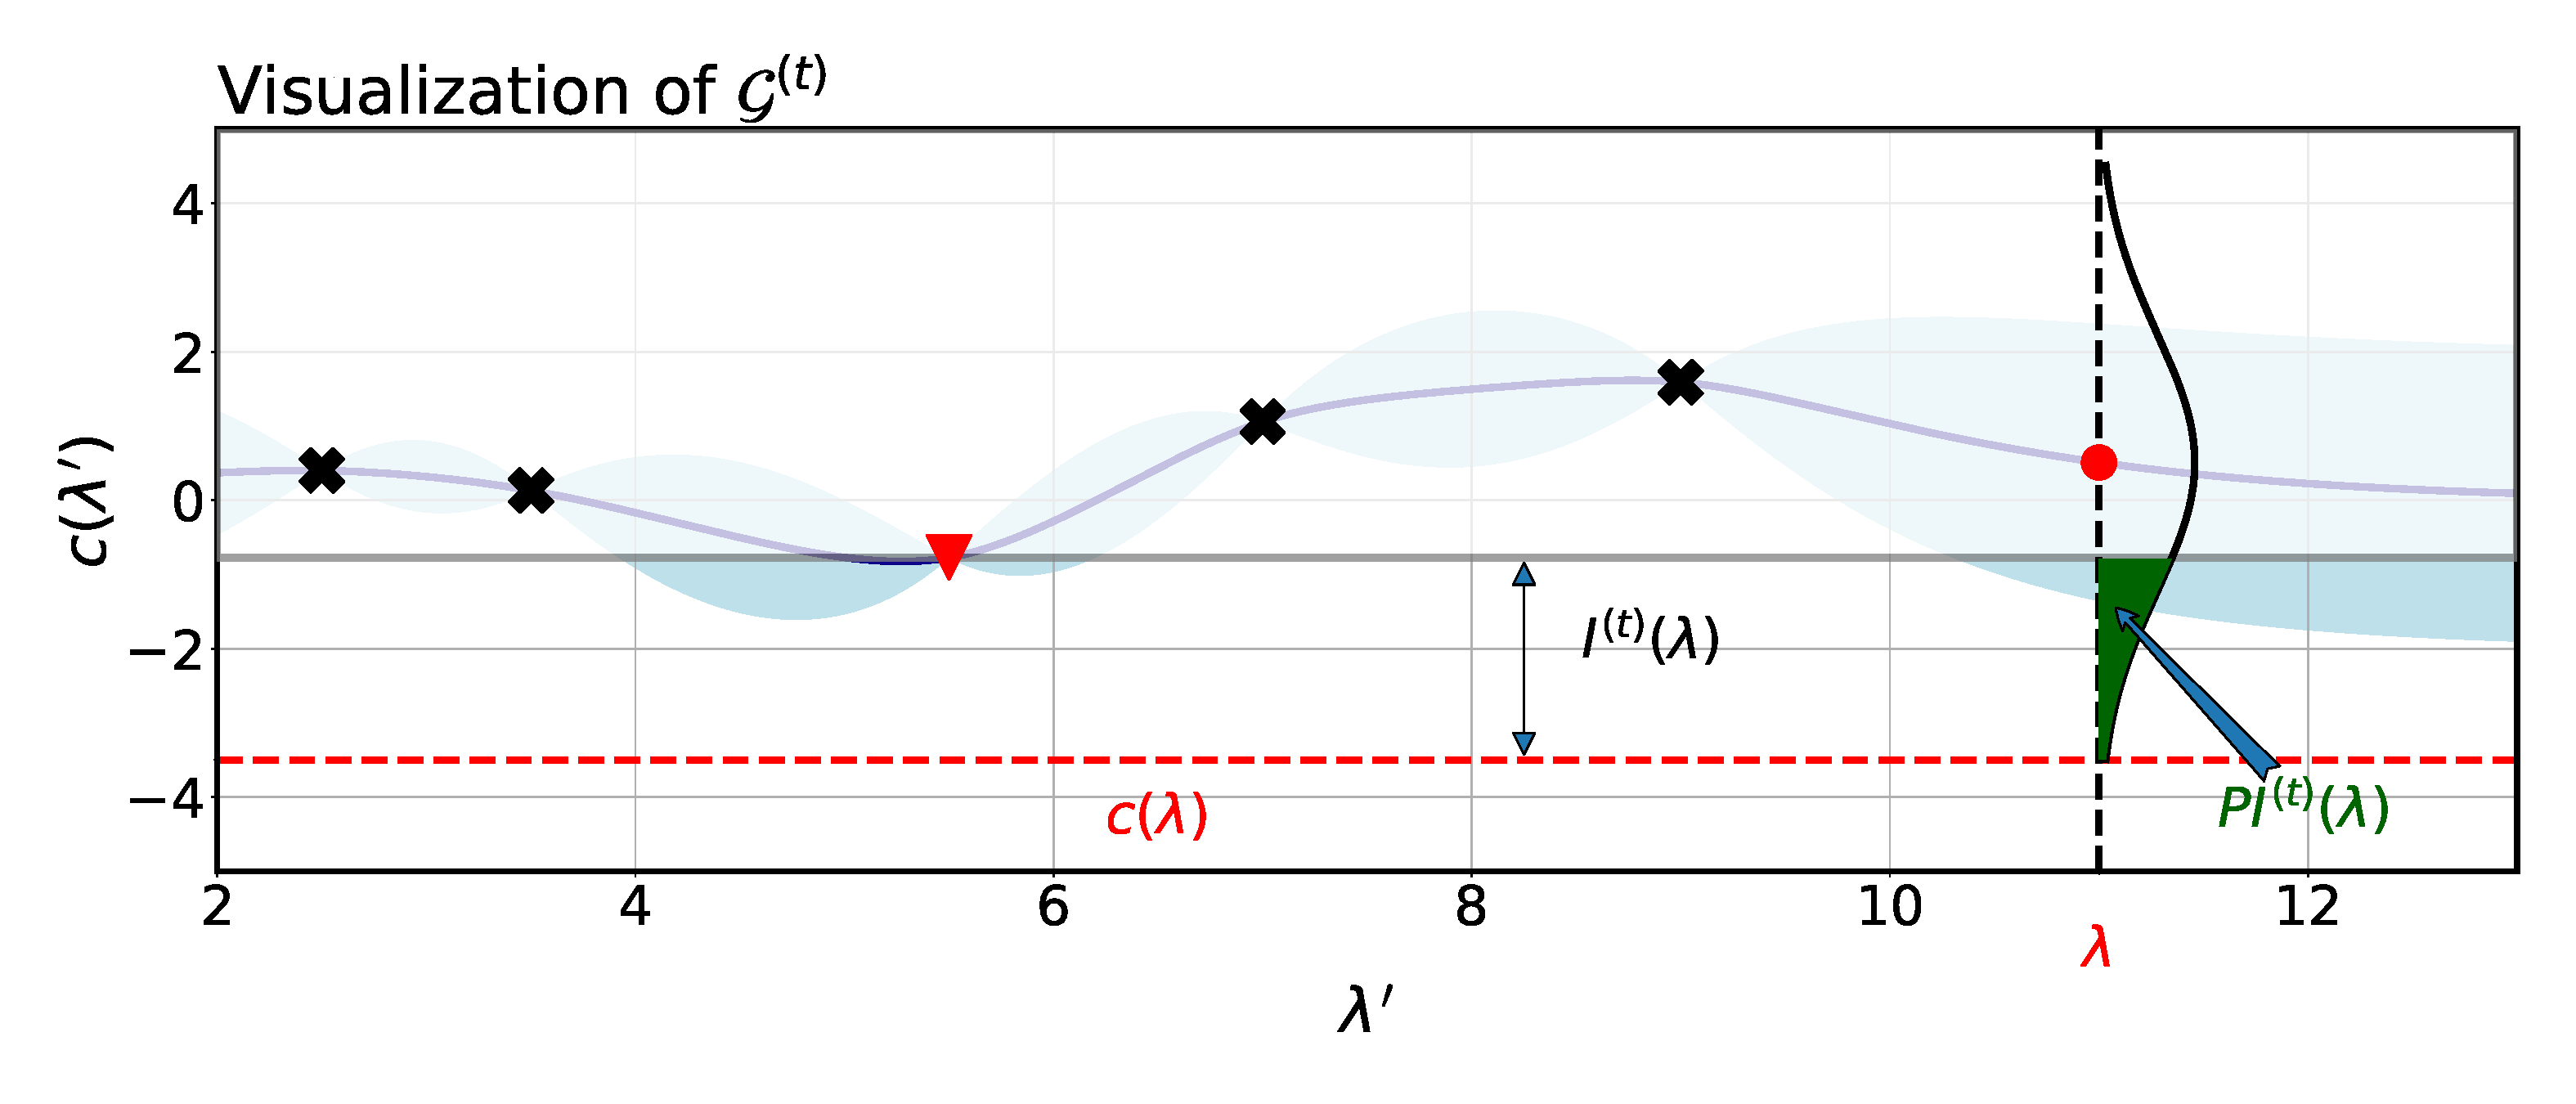
\includegraphics[width=\linewidth, height=0.7\textheight, keepaspectratio=true]{images/acq_func_images/ei/ei_7.pdf}};
    \node<.> [below=0.01\belowcaptionskip of img7, align=center]{Now consider the likelihood of a larger improvement.};
    
    \node<+> (img8) {\includegraphics[width=\linewidth, height=0.7\textheight, keepaspectratio=true]{images/acq_func_images/ei/ei_8.pdf}};
    \node<.> [below=-0.01\belowcaptionskip of img8, align=center]{Larger improvements are more likely in areas of high uncertainty.\\ To compute $\E[I(\conf)]$, intuitively, we sum $p(\cost \mid \conf) \times I_\cost$ over all possibles values of $\cost$.
    %\\We can thus use $\surro(\conf) = \normaldist( \mean(\conf), \variance(\conf))$ to calculate $\E[\iter{I}(\conf)]$.
    };

  \end{tikzpicture}
% \end{figure}

\end{frame}
%-----------------------------------------------------------------------
\begin{frame}[c]{Expected Improvement (EI): Formal Definition}
%\framesubtitle{Expected Improvement - Choosing a candidate}
    \begin{itemize}\abovedisplayskip=0em\belowdisplayskip=-0.75em
        \item We define the one-step positive \alert{improvement over the current incumbent} as
        \smallskip
        \[
            \alert{\iter{I}(\conf) = \max(0, \cost_{inc} - \cost(\conf))}
        \]
%        \comment{This is probably a great time to point out, once again, that because I is defined in terms of the actual cost function, we cannot directly compute it.}
        \smallskip
        \item Expected Improvement is then defined as \alert{\[\iter{\acq}_{EI}(\conf) = \E[\iter{I}(\conf)] = \int_{-\infty}^{\infty} \iter{p}(\cost \mid \conf) \times \iter[\bocount]{I}(\conf)\;\; d\cost.\]}
        \pause
        \smallskip
        \item Since the posterior distribution of $\surro(\conf)$ is a Gaussian, EI can be computed in closed form (see exercise):
        
%        \comment{Maybe emphasize that this is actually how and where the dependence on the actual cost function is replaced with a dependence on the surrogate.}
        \begin{align*}
            \alert{\iter{\acq}_{EI}(\conf)} &\alert{=} 
            \begin{cases}
                \alert{\iter{\stddev}(\conf)[Z\cdf(Z) + \pdf(Z)]}, & \text{if }\iter{\stddev}(\conf) > 0 \\
                0 & \text{if }\iter{\stddev}(\conf) = 0,
            \end{cases}\\
            \text{where }Z &=\dfrac{\cost_{inc} - \iter{\mean}(\conf) - \xi}{\iter{\stddev}(\conf)}
            \text{ and } \xi \text{ is an optional exploration parameter.}
        \end{align*}
%            \comment{I believe I needed to switch the signs of $\cost(\cdot)$ and $\mean(\cdot)$ as compared to the reference paper in order to accommodate for our convention of minimization/maximization. Please cross-check!}
    \pause
    \bigskip
    \[\boxed{\text{Choose}\;\;\bonextsample \in \argmax_{\conf\in\pcs}(\iter{\acq}_{EI}(\conf))}
    \]
    \end{itemize}
\end{frame}
%-----------------------------------------------------------------------
%\begin{frame}[c]{Computationally Cheap Acquisition Functions - EI}
%\framesubtitle{Expected Improvement - Choosing a candidate}
%\comment{Verify if formulae agree with minimizing the surrogate.}
%    \begin{itemize}\abovedisplayskip=0pt\belowdisplayskip=-0.5em
%        \item[] We first define one-step improvement over the current incumbent, as
%        \smallskip
%        \[
%            \iter{I}(\conf) = \max(0, \cost(\incumbent[\bocount-1]) - \cost(\conf)), \quad\incumbent[\bocount-1]\in\argmin_{\conf'\in\iter[\bocount-1]{\dataset}}\obs[\conf']\in\iter[\bocount-1]{\dataset}
%        \]
%        \comment{This is probably a great time to point out, once again, that because I is defined in terms of the actual cost function, we cannot directly compute it.}
%        \fhpause
%        \medskip
%        \item[] Expected Improvement is then defined as
%        \begin{align*}
%            \iter{\acq}_{EI}(\conf) &= \E[\iter{I}(\conf)]\\
%            &= \int_{\iter{I}=0}^{\iter{I}=\infty}\iter{I} P(\iter{I})d\iter{I}
%        \end{align*}
%        \fhpause
%        \medskip
%        \item[]Since the posterior distribution of the surrogate is a Gaussian, it can be shown that the distribution on $\iter{I}(\conf)$ is also a Gaussian, defined as
%        \[
%            P(\iter{I}) =
%                \dfrac{1}{\sqrt{2\pi}\iter{\stddev}(\conf)}\exp{\left[-\dfrac{{(\cost(\incumbent[\bocount-1])-\iter{\mean}(\conf)-\iter{I})}^2}{2\iter{\left(\variance\right)}(\conf)}
%            \right]}
%        \]
%        \comment{Maybe emphasize that this is actually how and where the dependence on the actual cost function is replaced with a dependence on the surrogate.}
%    \end{itemize}
%\end{frame}
%-----------------------------------------------------------------------
% \begin{frame}[c]{Computationally Cheap Acquisition Functions - EI}
% \framesubtitle{Expected Improvement - Choosing a candidate}
%     \begin{align*}
%         \action<+->{\iter{\acq}_{EI}(\conf) &= \int_{\iter{I}=0}^{\iter{I}=\infty}\iter{I} \dfrac{1}{\sqrt{2\pi}\iter{\stddev}(\conf)}\exp{-\dfrac{{(\cost(\incumbent[\bocount-1])-\iter{\mean}(\conf)-\iter{I})}^2}{2\iter{\left(\variance\right)}(\conf)}}d\iter{I}\\}
%         \action<+->{&= 
%             \begin{cases}
%                 (\cost(\incumbent) - \iter{\mean}(\conf) - \xi)\cdf(Z) + \iter{\stddev}(\conf) \pdf(Z), & \text{if }\iter{\stddev}(\conf) > 0 \\
%                 0 & \text{if }\iter{\stddev}(\conf) = 0
%             \end{cases}\\}
%         \action<+->{\intertext{where }Z} \action<.->{&=\dfrac{\cost(\incumbent) - \iter{\mean}(\conf) - \xi}{\iter{\stddev}(\conf)}}
%     \action<+->{\Aboxed{\bonextsample \in \argmax_{\conf\in\pcs}(\iter{\acq}_{EI}(\conf))}}
%     \end{align*}
% %    \comment{Source: Tutorial by Brochu et al.: https://arxiv.org/pdf/1012.2599.pdf }
% \end{frame}
%-----------------------------------------------------------------------
%\begin{frame}[c]{Computationally Cheap Acquisition Functions - EI}
%\framesubtitle{Expected Improvement - Choosing a candidate}
%    \begin{align*}
%        \action<+->{\iter{\acq}_{EI}(\conf) &= \int_{\iter{I}=0}^{\iter{I}=\infty}\iter{I} \dfrac{1}{\sqrt{2\pi}\iter{\stddev}(\conf)}\exp{-\dfrac{{(\cost(\incumbent[\bocount-1])-\iter{\mean}(\conf)-\iter{I})}^2}{2\iter{\left(\variance\right)}(\conf)}}d\iter{I}\\}
%        \action<+->{&= 
%            \begin{cases}
%                \iter{\stddev}(\conf)[Z\cdf(Z) + \pdf(Z)], & \text{if }\iter{\stddev}(\conf) > 0 \\
%                0 & \text{if }\iter{\stddev}(\conf) = 0
%            \end{cases}\\
%            \intertext{where }Z &=\dfrac{\cost(\incumbent[\bocount-1]) - \iter{\mean}(\conf) - \xi}{\iter{\stddev}(\conf)}}
%            \comment{I believe I needed to switch the signs of $\cost(\cdot)$ and $\mean(\cdot)$ as compared to the reference paper in order to accommodate for our convention of minimization/maximization. Please cross-check!}
%    \action<+->{\Aboxed{\text{Choose}\,\bonextsample \in \argmax_{\conf\in\pcs}(\iter{\acq}_{EI}(\conf))}}
%    \end{align*}
%    \comment{Source: Tutorial by Brochu et al.: https://arxiv.org/pdf/1012.2599.pdf }
%\end{frame}
%-----------------------------------------------------------------------
\begin{frame}[t]{Lower/Upper Confidence Bounds (LCB/UCB): Concept}

% \begin{figure}
  \centering
  \begin{tikzpicture}
    \node<+> (img1) {\includegraphics[width=\linewidth, height=0.7\textheight, keepaspectratio=true]{images/acq_func_images/lcb/lcb_1.pdf}};
    \node<.> [below=0.01\belowcaptionskip of img1, align=center]{Given the surrogate fit at iteration $\bocount$};
    %fit on dataset $\iter[\bocount-1]{\dataset}$};
    \node<+> (img2) {\includegraphics[width=\linewidth, height=0.7\textheight, keepaspectratio=true]{images/acq_func_images/lcb/lcb_2.pdf}};
    \node<.> [below=0.01\belowcaptionskip of img2, align=center]{Lower Confidence Bound, $\mean(\conf)-\alpha\stddev(\conf)$ (here, for $\alpha=3$)};
  \end{tikzpicture}
% \end{figure}

\end{frame}
%-----------------------------------------------------------------------
\begin{frame}[c]{Lower/Upper Confidence Bounds (LCB/UCB): Formal Definition}
\begin{itemize}
    \item We define the \alert{Lower Confidence Bound} as
    \[\alert{\iter{\acq}_{LCB}(\conf) = \iter{\mean}(\conf) - \alpha\iter{\stddev}(\conf)},\quad\alpha\geq0\]

\bigskip
    \item One can schedule $\alpha$ (e.g., increase it over time \lit{\href{https://arxiv.org/pdf/0912.3995.pdf}{Srinivas et al. 2009}})

\[
    \boxed{\text{Choose}\;\;\bonextsample \in \argmax_{\conf\in\pcs}\left(\alert{-} \iter{\acq}_{LCB}(\conf)\right)}
\]

\end{itemize}
    \bigskip
    \pause
    
    \begin{itemize}
    
    
        \item Note: when one aims to \alert{maximize} the objective function, one would use \alert{UCB} instead
        \begin{itemize}
            \item $\iter{\acq}_{UCB}(\conf)) = \iter{\mean}(\conf) + \alpha\iter{\stddev}(\conf)$ 
            \item For UCB, one would choose $\bonextsample \in \argmax_{\conf\in\pcs}( \iter{\acq}_{UCB}(\conf))$ 
        \end{itemize}
    \end{itemize}
   
%    \item It has been shown that using the acquisition function
%    \[\iter{\acq}_{GP-LCB}(\conf) = \iter{\mean}(\conf) - \sqrt{\nu\tau_t}\iter{\stddev}(\conf), \quad\nu>0,\] asymptotically results in zero cumulative regret with the appropriate choice of parameters $\tau$ and $\nu$ \lit{\href{https://arxiv.org/pdf/0912.3995.pdf}{Srinivas et al. 2009}}.}
%    \comment{Trying to further explain the difference between LCB and GP-LCB's parameters would've overwhelmed the intuitiveness of the slide. Instead, a quick verbal note on the difference and pointing out the reference paper by Srinivas et al. for further reading should suffice.}
    %\comment{Source: Tutorial by Brochu et al.: https://arxiv.org/pdf/1012.2599.pdf }
\end{frame}
%-----------------------------------------------------------------------
\begin{frame}[t]{Thompson Sampling (TS): Concept}

% \begin{figure}
  \centering
  \begin{tikzpicture}
    \node<+> (img1) {\includegraphics[width=\linewidth, height=0.7\textheight, keepaspectratio=true]{images/acq_func_images/ts/ts_1.pdf}};
    \node<.> [below=0.01\belowcaptionskip of img1, align=center]{Given the surrogate at iteration $\bocount$ fit on dataset $\iter[\bocount-1]{\dataset}$};
    \node<+> (img2) {\includegraphics[width=\linewidth, height=0.7\textheight, keepaspectratio=true]{images/acq_func_images/ts/ts_2.pdf}};
    \node<.> [below=0.01\belowcaptionskip of img2, align=center]{Draw a sample $g$ from the predictive surrogate model};
    \node<+> (img3) {\includegraphics[width=\linewidth, height=0.7\textheight, keepaspectratio=true]{images/acq_func_images/ts/ts_3.pdf}};
    \node<.> [below=0.01\belowcaptionskip of img3, align=center]{Then choose the minimum of this sample to evaluate at next};
  \end{tikzpicture}
% \end{figure}

\end{frame}
%-----------------------------------------------------------------------
% \begin{frame}[c]{Computationally Cheap Acquisition Functions - TS}
% \framesubtitle{Thompson Sampling - Gist}
% 
% \begin{itemize}
%     \item Draw a sample $g$ from the GP $\iter{\gp}$.
%     \item Choose $\bonextsample=\argmin_{\conf\in\pcs}(g(\conf))$
% \end{itemize}
% \end{frame}
%-----------------------------------------------------------------------
\begin{frame}[c]{Thompson Sampling (TS): Pseudocode}

\begin{center}
\begin{minipage}{0.75\textwidth}
\comment{Fix algorithm numbering}
\begin{algorithm}[H]
    %\DontPrintSemicolon
    \LinesNumbered
%    \SetAlgoLined
    \setcounter{AlgoLine}{0}
    \SetKwInOut{Require}{Require}
    \SetKwInOut{Result}{Result}
    
    \Require{Search space $\pcs$, 
    		cost function $\cost$, 
    		surrogate model $\surro$,
    		maximal number of function evaluations $\bobudget$}
\Result{Best observed configuration $\finconf$ according to $\iter[\bobudget]{\dataset}$ or $\gp$}    
	Initialize data $\iter[0]{\dataset}$ with initial observations\;% \leftarrow \varnothing$\; 
    
    \For{$\bocount=1$ \KwTo $\bobudget$}{
    
		Fit predictive model $\iter[\bocount]{\surro}$ on $\iter[\bocount-1]{\dataset}$\;
    
        \textcolor{blue}{Sample a function from the surrogate: $g\sim\iter{\surro}$}\;
    
        \textcolor{blue}{Select next query point: $\bonextsample \in \argmin_{\conf\in\pcs}g(\conf)$}\;
    
        Query $\bonextobs$\;

    	Update data: $\iter[\bocount]{\dataset} \leftarrow \iter[\bocount-1]{\dataset} \cup \{\langle \bonextsample, \bonextobs \rangle \}$\;
        }
    \caption*{Bayesian Optimization using Thompson Sampling}
\end{algorithm}
\end{minipage}
\end{center}
%\comment{Source: Paper, Kandasamy et al, http://proceedings.mlr.press/v84/kandasamy18a/kandasamy18a.pdf}
\end{frame}
%-----------------------------------------------------------------------
\begin{frame}[c]{Questions to Answer for Yourself / Discuss with Friends}

\begin{itemize}
%PI
    \item \alert{Discussion.} How would you set the exploration parameter $\xi$ for PI if you want to avoid too incremental improvements?
\medskip
%EI
    \item \alert{Derivation.} Derive the closed form solution of expected improvement.
\medskip
    \item \alert{Discussion.} In which situations would EI perform substantially differently than PI?
%LCB
%TS
\end{itemize}

\end{frame}
\end{document}
    %-----------------------------------------------------------------------
\subsection{Advanced Acquisition Functions}
\begin{frame}[c]{Advanced Acquisition Functions}
\framesubtitle{Contents}
\pause
\begin{itemize}
    \item Concept: One-step look-ahead.
    \item Knowledge Gradient
    \item Entropy Search
    \item \emph{Maybe mention that we are now going to actually trust our surrogate to somewhat accurately model the underlying objective function (or that we are now risk-neutral) - thus relaxing one of the constraints mentioned in the very beginning of the section on Acquisition Functions.}
\end{itemize}
\end{frame}

%-----------------------------------------------------------------------

\begin{frame}[c]{Advanced Acquisition Functions}
%\framesubtitle{Knowledge Gradient - Concept}
\framesubtitle{One-Step Look Ahead}
\pause

\begin{figure}
  \centering
  \begin{tikzpicture}
    \node<+> (img1) {\includegraphics[width=.7\linewidth, height=0.7\textheight, keepaspectratio=true]{latex_main/images/placeholder.png}};
    \node<.> [below=0.01\belowcaptionskip of img1, align=center]{Once more, assume such a surrogate function GP $\iter{\gp}(\cdot)$ at time-step $\bocount$.};
    
    \node<+> (img2) {\includegraphics[width=.7\linewidth, height=0.7\textheight, keepaspectratio=true]{latex_main/images/placeholder.png}};
    \node<.> [below=0.01\belowcaptionskip of img2, align=center]{\emph{If} we evaluate $\cost(\cdot)$ at a random configuration $\conf$, $\iter[\bocount+1]{\gp}(\cdot\given {\conf})$ \emph{might} look like this. \\ \emph{Show what GP might look like at time-step $\bocount+1$.}};
    
    \node<+> (img3) {\includegraphics[width=.7\linewidth, height=0.7\textheight, keepaspectratio=true]{latex_main/images/placeholder.png}};
    \node<.> [below=0.01\belowcaptionskip of img3, align=center]{Mean - $\iter[\bocount+1]{\mean} \given_{\conf}$, Variance - $\iter[\bocount+1]{\left(\variance\right)} \given_{\conf}$, Minimum of the mean function - $\iter[\bocount+1]{\left(\mean^*\right)} \given_{\conf}$. \\\emph{Point out that all these quantities are now conditionally dependent on our choice of $\conf$}};
    
    \node<+> (img4) {\includegraphics[width=.7\linewidth, height=0.6\textheight, keepaspectratio=true]{latex_main/images/placeholder.png}};
    \node<.> [below=0.01\belowcaptionskip of img4, align=center]{This distribution is purely hypothetical - as shown by the conditional - \\and is called a one-step look-ahead. \emph{Just a re-statement of the GP's conditional nature at $\bocount+1$}};
  \end{tikzpicture}
\end{figure}

\end{frame}
%-----------------------------------------------------------------------

\begin{frame}[c]{Advanced Acquisition Functions - KG}
%\framesubtitle{Knowledge Gradient - Concept}
\framesubtitle{Knowledge Gradient - Concept}
\pause

\begin{figure}
  \centering
  \begin{tikzpicture}
    \node<+> (img1) {\includegraphics[width=.7\linewidth, height=0.7\textheight, keepaspectratio=true]{latex_main/images/placeholder.png}};
    \node<.> [below=0.01\belowcaptionskip of img1, align=center]{Once more, assume such a surrogate function GP $\iter{\gp}(\cdot)$ at time-step $\bocount$.};
    
    \node<+> (img2) {\includegraphics[width=.7\linewidth, height=0.6\textheight, keepaspectratio=true]{latex_main/images/placeholder.png}};
    \node<.> [below=0.01\belowcaptionskip of img2, align=center]{Given that we are risk-neutral, the configuration corresponding to the minimum \\of the mean function, $\iter{\left(\mean^*\right)}$, is the best choice here.};
    
    \node<+> (img3) {\includegraphics[width=.7\linewidth, height=0.7\textheight, keepaspectratio=true]{latex_main/images/placeholder.png}};
    \node<.> [below=0.01\belowcaptionskip of img3, align=center]{We perform a one-step look-ahead to get $\iter[\bocount+1]{\gp}(\cdot\given {\conf})$.};
    
    \node<+> (img4) {\includegraphics[width=.7\linewidth, height=0.7\textheight, keepaspectratio=true]{latex_main/images/placeholder.png}};
    \node<.> [below=0.01\belowcaptionskip of img4, align=center]{The best risk-neutral choice is again given by the minimum \\of the new conditional mean function - $\iter[\bocount+1]{\left(\mean^*\right)} \given_{\conf}$.};
    
    \node<+> (img5) {\includegraphics[width=.7\linewidth, height=0.7\textheight, keepaspectratio=true]{latex_main/images/placeholder.png}};
    \node<.> [below=0.01\belowcaptionskip of img5, align=center]{The expected value of the improvement in cost - from $\iter{\left(\mean^*\right)}$ to $\iter[\bocount+1]{\left(\mean^*\right)}$ - is \\ Knowledge Gradient. \emph{Show side-by-side comparison of the two GPs}};
  \end{tikzpicture}
\end{figure}

\end{frame}
%-----------------------------------------------------------------------
\begin{frame}[c]{Advanced Acquisition Functions - KG}
\framesubtitle{Knowledge Gradient - Choosing a candidate}
\pause
\begin{itemize}\abovedisplayskip=0.5em\belowdisplayskip=0.5em
    \action<+->{\item Given a GP $\iter{\gp}$ fit on $\iter[\bocount-1]{\dataset}$, on the $\bocount\,$th iteration we have}
    \action<+->{\[\iter{\left(\mean^*\right)} = \max_{\conf'\in\pcs}(\iter{\mean}(\conf'\given{\dataset_{\bocount-1}}))\]}
    \action<+->{\item If we choose a candidate $\bonextsample=\conf$ to evaluate $\cost(\cdot)$ at,}
    %\action<+->{\[\dataset_{\bocount}\given{\conf} = \{(\conf_1, \boobs_1),\dots,(\conf_{\bocount-1}, \boobs_{\bocount-1})\}\cup\{(\iter{\conf},\iter{\boobs})\given{\bonextsample=\conf}\}.\]}
    \action<+->{\[\iter{\dataset}\given\conf = \iter[\bocount-1]{\dataset}\cup\{\langle\bonextsample,\,\bonextobs\rangle\given{\bonextsample=\conf}\}.\]}
    \action<+->{\item Thus, if we hypothesize about the $\bocount+1\,$th iteration, we would get}
    \action<+->{\[\iter[\bocount+1]{\left(\mean^*\right)} \given_{\conf} = \max_{\conf'\in\pcs}(\iter[\bocount+1]{\mean}(\conf'\given{\iter{\dataset},\bonextsample=\conf}))\]}
\end{itemize}
\comment{Source:https://arxiv.org/pdf/1807.02811.pdf}
\end{frame}
%-----------------------------------------------------------------------
\begin{frame}[c]{Advanced Acquisition Functions - KG}
\framesubtitle{Knowledge Gradient - Choosing a candidate}
\begin{itemize}\abovedisplayskip=1em\belowdisplayskip=0em
    \action<+->{\item In a risk-neutral setting, $\iter{\left(\mean^*\right)}$ and $\iter[\bocount+1]{\left(\mean^*\right)}$ are the global optima for $\iter{\mean}$ and $\iter[\bocount+1]{\mean}\given_{\conf}$ respectively.}
    \action<+->{\item Thus, the conditional improvement in the cost (adjusted for maximization) is \[\iter{\left(\mean^*\right)} - \left.\iter[\bocount+1]{\left(\mean^*\right)} \right|_{\bonextsample=\conf}\]}
    \action<+->{\item We cannot directly compute this improvement, but we can compute its expected value, which we call Knowledge Gradient:}
    \action<+->{\[\iter{KG}(\conf) = \E\left[ \iter{\left(\mean^*\right)} - \left. \iter[\bocount+1]{\left(\mean^*\right)} \right|_{\bonextsample=\conf} \right]\]}
    \action<+->{\item Finally, \[\boxed{\bonextsample = \argmax_{\conf\in\pcs}(\iter{KG}(\conf))}\]}
\end{itemize}
\comment{Source:https://arxiv.org/pdf/1807.02811.pdf}
\end{frame}
%-----------------------------------------------------------------------
\begin{frame}[c]{Advanced Acquisition Functions - ES}
\framesubtitle{Entropy Search - Concept}
\pause

\begin{figure}
  \centering
  \begin{tikzpicture}
    \node<+> (img1) {\includegraphics[width=.7\linewidth, height=0.6\textheight, keepaspectratio=true]{latex_main/images/placeholder.png}};
    \node<.> [below=0.01\belowcaptionskip of img1, align=center]{We consider the global optimum's position to be a random variable $\conf^*$, \\with uniform prior probability. \emph{Show the probability distribution below the GP throughout ES}};
    
    \node<+> (img2) {\includegraphics[width=.7\linewidth, height=0.7\textheight, keepaspectratio=true]{latex_main/images/placeholder.png}};
    \node<.> [below=0.01\belowcaptionskip of img2, align=center]{The minimum of a sample from the GP $\iter{\gp}$ provides some evidence for where $\conf^*$ may lie. \\\emph{Visualization for demonstrative purposes only, not actual implementation.}};
    
    \node<+> (img3) {\includegraphics[width=.7\linewidth, height=0.7\textheight, keepaspectratio=true]{latex_main/images/placeholder.png}};
    \node<.> [below=0.01\belowcaptionskip of img3, align=center]{Each new sample provides more information about where the global minimum lies - \\i.e. has an assosciated \emph{information gain}.};
    
    \node<+> (img4) {\includegraphics[width=.7\linewidth, height=0.7\textheight, keepaspectratio=true]{latex_main/images/placeholder.png}};
    \node<.> [below=0.01\belowcaptionskip of img4, align=center]{After $S$ such samples, we can narrow down the approximate location of the global minimum\\ i.e. reduce entropy of the search space.};
  \end{tikzpicture}
\end{figure}

\end{frame}
%----------------------------------------------------------------------
\begin{frame}[c]{Advanced Acquisition Functions - ES}
\framesubtitle{Entropy Search - Choosing a candidate}
\begin{itemize}
    \item Provide formulae for entropy search - pseudocode for the sampling-based version, formula for overall entropy search (integral of H) only
    \item Mention existence of more complicated but efficient search procedure, mention differences.
    \item Mention: Repeated Thompson Sampling is an approximation to sampling based entropy-search.
    \item Provide link to paper.
\end{itemize}
\comment{Source:https://arxiv.org/pdf/1807.02811.pdf}
\end{frame}
%-----------------------------------------------------------------------
    \videotitle{Surrogate Models}

%-----------------------------------------------------------------------
\myframetop{Desiderata for Surrogate Models in Bayesian Optimization}{

    \begin{columns}[T] % align columns
    \begin{column}{.48\textwidth}
    \only<1-2>{
        \begin{block}{In all cases}
        \begin{itemize}
        	\item Regression model with uncertainty estimates
        	\item Accurate predictions
        \end{itemize}
        \end{block}
    }
    \only<2-2>{
        \begin{block}{Depending on the application}
        \begin{itemize}
        	\item Is cheap to train
        	\item Scales well in the number of data points
        	\item Scales well in the number of dimensions
        	\item Can handle different types of inputs (categorical and continuous)
        \end{itemize}
        \end{block}
    }
    \end{column}%
    
    \hfill%
    
    \begin{column}{.48\textwidth}
    \bigskip
    \bigskip
    %\only<1-1>{\includegraphics[width=1.\textwidth]{images/bo_loop_overview/03_mean.png}}
    %\only<2-6>{
    \includegraphics[width=\textwidth]{images/bo_loop_overview/Uncertainty.pdf}
    %}
    
    \end{column}%
    \end{columns}
}
%-----------------------------------------------------------------------

%-----------------------------------------------------------------------
%-----------------------------------------------------------------------
\begin{frame}[c]{Overview of the Surrogate Models We'll Discuss}

%\begin{columns}[T] % align columns
%\begin{column}{.38\textwidth}
%\begin{minipage}[c][.6\textheight][c]{\linewidth}
\begin{itemize}
	\item Gaussian Processes \note[item]{(quite common)}
	\item Random Forests \note[item]{(our default choice)}
	\item Bayesian Neural Networks \note[item]{(recent trend)}

\end{itemize}
%\end{minipage}
%\end{column}%

%\hfill%
%\begin{column}{.58\textwidth}
%
%\begin{columns}[T] % align columns
%\begin{column}{.48\textwidth}
%    \includegraphics[width=1.\textwidth]{images/surrogate_models/uncertainty_gp.jpg}
%\end{column}%
%
%\hfill%
%
%\begin{column}{.48\textwidth}
%    \includegraphics[width=1.\textwidth]{images/surrogate_models/uncertainty_forest.jpg}
%\end{column}%
%\end{columns}
%
%\vspace*{\fill}
%\begin{center}
%  \includegraphics[width=.6\textwidth]{images/surrogate_models/uncertainty_dngo.jpg}
%  
%\end{center}
%\vspace*{\fill}
%
%\end{column}%
%\end{columns}
%
%\hspace{5.5cm}\footnotesize{Image source: \lit{\href{}{A. Klein: Introduction Automated Machine Learning}}}


\end{frame}
%-----------------------------------------------------------------------
\begin{frame}[c]{Gaussian Processes (GPs): Reminder of Pros and Cons}

\begin{columns}[T] % align columns
\begin{column}{.48\textwidth}

    \begin{block}{Advantages}
    \begin{itemize}
    	\item Smooth and reliable uncertainty estimates 
		\item Strong sample efficiency
    	\item We can encode expert knowledge about the design space in the kernel 
    \end{itemize}
    \end{block}
\bigskip
\fhpause
\hspace*{0.5cm}These advantages make GPs the\\
\hspace*{0.5cm}\alert{most commonly-used model\\
\hspace*{0.5cm}in Bayesian optimization}

\end{column}%

\hfill%
\fhpause

\begin{column}{.48\textwidth}
    \begin{block}{Disadvantages}
    \begin{itemize}
    	\item Performance can be quite sensitive to the choice of kernel
    	\note[item]{(if we don't optimize small-dimensional, continuous functions)}
    	\item Cost scales cubically with the number of observations 
    	\item Weak performance for high dimensionality
    	\note[item]{(because of inverting the kernel)}
    	\item Not easily applicable in discrete or conditional spaces 
    	\item Sensitive to its own hyperparameters
    \end{itemize}
\end{block}

\end{column}
\end{columns}

\note[item]{
	\begin{itemize}
		 \item e.g., special kernels for categorical hyperparameters and\\ conditional dependencies
	\end{itemize}
}
	
\note[item]{
    \begin{itemize}
    	\item to address this issue, there are sparse GPs\\ \lit{Snelson and Ghahramani. 2005}
    \end{itemize}
}

\end{frame}
%-----------------------------------------------------------------------

%-----------------------------------------------------------------------
%-----------------------------------------------------------------------
%\begin{frame}[c]{Gaussian Processes - reminder}
%
%\begin{itemize}
%    \item<1-3> The prior is a GP with constant mean and variance; draws are jointly Gaussian
%    \item<2-3> The kernel (covariance) function $K$ tells us how correlated the function values at two points are
%    \item<3-3> The posterior is also a GP, with predictive distribution:
 %   \begin{equation*}
 %        P(\func_{\bocount+1} \vert \dataset_{1:\bocount}, \conf_{\bocount+1}) =  \mathcal{N}(\mean_{\bocount}(\conf_{\bocount+1}), \variance_{\bocount}(\conf_{\bocount+1}))
 %   \end{equation*}
 %   \begin{equation*}
 %       \mean_{\bocount}(\conf_{\bocount+1}) = \bm{k}^{T} \bm{K}^{-1} \bm{\func_{1:\bocount}}
 %   \end{equation*}
 %   \begin{equation*}
 %       \variance_{\bocount}(\conf_{\bocount+1}) = k(\conf_{\bocount+1}, \conf_{\bocount+1}) - \bm{k}^{T} \bm{K}^{-1} \bm{k}
 %   \end{equation*}
%\end{itemize}
%
%\note[item]{for the review of GPs - Rasmussen and Williams}
%
%\end{frame}
%-----------------------------------------------------------------------
 
% %-----------------------------------------------------------------------
% %-----------------------------------------------------------------------
% \begin{frame}[c]{Surrogate Models: GPs - kernel hyperparameters}

% \begin{itemize}
%     \item After choosing the kernel, we must also manage the hyperparameters that govern its behaviour, as well as that of the mean function.  \fhpause
%     \item For our problems of interest, typically we have $D + 3$ GPs hyperparameters:  
%     \begin{itemize}
%         \item $D$ length scales $\theta_{1:D}$, 
%         \item the covariance amplitude $\theta_{0}$, 
%         \item the observation noise $\noise$, 
%         \item a constant mean $\mean$. 
%     \end{itemize}
% \end{itemize}

% \end{frame}
% %-----------------------------------------------------------------------


%-----------------------------------------------------------------------
%-----------------------------------------------------------------------
\begin{frame}[c]{Gaussian Processes (GPs): Kernel Hyperparameters}

\begin{columns}[T] % align columns
\begin{column}{.6\textwidth}
\begin{itemize}
    \item We could optimize GP hyperparameters (maximum likelihood, MLE, or maximum a posteriori, MAP)


    \item<+-> But \alert{sampling} GP  hyperparameters from the posterior distribution performs better; e.g., via \alert{Markov-Chain Monte-Carlo (MCMC)}


    \item<+-> \alert{Marginalize} over GP hyperparameters $\theta$ and compute an \alert{integrated acquisition function}:
        \begin{equation*}
        \begin{aligned}
            \Bar{\acq}(\conf) = \int \acq (\conf, \surro_\theta)p(\theta)d\theta
        \end{aligned}
        \end{equation*}

 
    \item<+-> Downside: computational expense
    \myit{
        \item MCMC is computationally expensive
        \item Acquisition function now has to be calculated for each sample
    }
\end{itemize}
\end{column}
%
\begin{column}{.4\textwidth}
\only<2->{
    \centering
    \includegraphics[width=0.7\textwidth]{images/surrogate_models/kernel_hp_mcmc.jpg}
    
    \footnotesize{Image source: \lit{\href{https://arxiv.org/pdf/1206.2944.pdf}{Snoek et al. 2012}}}
}


   
\end{column}

\end{columns}

\end{frame}
%-----------------------------------------------------------------------
\begin{frame}[c]{Random Forests (RFs): Reminder \& How To Compute Uncertainties}

\centering
    \includegraphics[width=0.5\textwidth]{images/surrogate_models/random_forest_pic}

\begin{columns}[T] % align columns
\begin{column}{.48\textwidth}

\begin{block}{RF Training}
\begin{itemize}
	\item Fit a set of \alert{randomized} regression trees
	\item Randomization via bootstrapping \& random selection of split variables / split points
	\item Each tree yields a possible explanation for the observations
\end{itemize}
\end{block}
\end{column}

\fhpause
\hfill

\begin{column}{.48\textwidth}
    \begin{block}{RF Prediction}
    \begin{itemize}
    	\item Predict with each tree
    	\item Aggregate predictions (e.g., average)
    	\item Uncertainty estimate:\\ \alert{empirical variance across tree predictions}
    \end{itemize}
    \end{block}
\end{column}
\end{columns}

\end{frame}
%-----------------------------------------------------------------------
\begin{frame}[c]{Random Forests (RFs): Impact of Basic Model Choices}
\vspace{-25pt}

\begin{columns}
\column{0.5\textwidth}

\begin{figure}[h]
\captionsetup[subfigure]{position=top}
\centering

\renewcommand{\thesubfigure}{a}
\subfloat[][no bootstrapping, \\ no random splits]{
\includegraphics[width=0.55\textwidth, clip]{images/surrogate_models/rf_noboot_middle_split.png}

}
\qquad
\renewcommand{\thesubfigure}{b}
\subfloat[][with bootstrapping, \\ no random splits]{
\includegraphics[width=0.55\textwidth, clip]{images/surrogate_models/rf_boot_middle_split.png}
}
\end{figure}

\column{0.5\textwidth}
\begin{figure}[h]
\captionsetup[subfigure]{position=top}
\centering

\fhpause
\renewcommand{\thesubfigure}{c}
\subfloat[][no bootstrapping, \\ with random splits]{
\includegraphics[width=0.55\textwidth, clip]{images/surrogate_models/rf_noboot_rand_split.png}

}
\qquad
\renewcommand{\thesubfigure}{d}
\subfloat[][with bootstrapping, \\ with random splits]{
\includegraphics[width=0.55\textwidth, clip]{images/surrogate_models/rf_boot_rand_split.png}
}

\end{figure}
\end{columns}

\end{frame}
%-----------------------------------------------------------------------
\begin{frame}[c]{Random Forests (RFs): Overview of Pros and Cons}

\begin{columns}[T] % align columns
\begin{column}{.48\textwidth}

    \begin{block}{Advantages}
    \begin{itemize}
        \item Cheap to train 
        \item Scales well with \#observations $n$: 
        \begin{itemize}
        	\item Fitting: $O(n \log n)$ 
        	\item Prediction: $O(\log n)$
        \end{itemize}
        \item Scales well with \#dimensions
        \item Training can be parallelized 
        \item Can easily handle conditional, categorical, continuous and discrete spaces 
        \item Quite robust against its own hyperparameters
    \end{itemize}
    \end{block}
\end{column}%

\hfill%
\fhpause

\begin{column}{.48\textwidth}
    \begin{block}{Disadvantages}
    \begin{itemize}
        \item Poor uncertainty estimates 
        \item Poor extrapolation (constant) 
    	\item Priors cannot be incorporated easily 
    \end{itemize}
    \end{block}

\fhpause
\bigskip
\bigskip
\hspace*{0.5cm}These qualities make RFs a \alert{robust} \\
\hspace*{0.5cm}\alert{option} for Bayesian optimization in \\ \hspace*{0.5cm}\alert{high dimensions}, for \alert{categorical spaces},\\
\hspace*{0.5cm}or when function evaluations are quite fast

\end{column}
\end{columns}

\end{frame}
%-----------------------------------------------------------------------
\begin{frame}[c]{Bayesian Neural Networks: Overview}

\begin{itemize}
    \item Neural networks are more flexible \& scalable than Gaussian processes 
    \item But for use in Bayesian optimization, neural networks need to be made probabilistic
    
\fhpause
    \item Bayesian deep learning aims to deal with all sources of uncertainty \fhpause
    \begin{itemize}
        \item E.g., we don't have a single weight vector anymore, but a distribution over weights
    \end{itemize}

\centering
\includegraphics[width=0.6\textwidth]{images/surrogate_models/bnn.jpg}

\footnotesize{Image source: \lit{\href{http://proceedings.mlr.press/v37/blundell15.pdf}{Blundell et al. 2015}}}

\end{itemize}



\end{frame}
%-----------------------------------------------------------------------
%\begin{frame}[c]{Surrogate Models: Bayesian Neural Networks - Idea}
%
%\begin{itemize}
%    \item Extend regression NNs to model uncertainty
%    \item Deal with all sources of parameter uncertainty
%    \item If possible, one would also deal with uncertainty about the network architecture
%     \begin{itemize}
%        \item For every architecture, one would still want to be Bayesian about its weights... 
%        \item Nobody is really Bayesian about architectures these days 
%        \item This has been too expensive; but that may change with efficient gradient-based architecture search methods...
%    \end{itemize}
%\end{itemize}
%
%\end{frame}

%-----------------------------------------------------------------------

\begin{frame}[c]{Simplest Way of Incorporating Uncertainty in Neural Networks: DNGO}


\begin{itemize}
    \item Fit a standard regression neural network to the data (with a linear output layer)
    \item Use the representation in the last hidden layer as \alert{basis functions $\phi(x)$} of the input $x$ 
    \item \alert{Use Bayesian linear regression with these basis functions} \fhpause
    \begin{itemize}
        \item The last layer is linear in its parameters $\theta$  
        \item Therefore, the Bayesian linear regression formulas work directly 
        \item Feasible in closed form, in time $O(N d^3)$, where $N$ is the number of data points\\ and $d$ is the number of hidden units in the last layer 
    \end{itemize}
    \item Not fully Bayesian yet, but already allows scalable Bayesian optimization \lit{\href{https://arxiv.org/pdf/1502.05700.pdf}{Snoek et al. 2015}}

\end{itemize}

%\vspace{1cm}
%\hspace{12cm}
%\lit{\href{https://arxiv.org/pdf/1502.05700.pdf}{Snoek et al. 2015}}

\end{frame}


%-----------------------------------------------------------------------

\begin{frame}[c]{Bayesian Optimization with BNNs: Overview of Existing Approaches}

\begin{itemize}
	    \item \lit{\href{https://arxiv.org/pdf/1502.05700.pdf}{Snoek et al. 2015}} Scalable Bayesian Optimization Using Deep Neural Networks (DNGO)
	    \item \lit{\href{https://papers.nips.cc/paper/6117-bayesian-optimization-with-robust-bayesian-neural-networks.pdf}{Springenberg et al. 2016}} Bayesian Optimization with Robust Bayesian Neural Networks
	    \item \lit{\href{https://arxiv.org/abs/1706.01825}{Hern\'andez-Lobato et al. 2017}} Parallel and Distributed Thompson Sampling for Large-scale Accelerated Exploration of Chemical Space
\bigskip
\fhpause
        \item \lit{\href{https://www.ismll.uni-hildesheim.de/pub/pdfs/schilling2015-ecml.pdf}{Schilling et al. 2015}} Hyperparameter Optimization with Factorized Multilayer Perceptrons
        \item \lit{\href{https://papers.nips.cc/paper/7917-scalable-hyperparameter-transfer-learning}{Perrone et al. 2018}} Scalable Hyperparameter Transfer Learning

\end{itemize}

\end{frame}
%-----------------------------------------------------------------------
\begin{frame}[c]{Bayesian Neural Networks (BNNs): Overview of Pros and Cons}

\begin{columns}[T] % align columns
\begin{column}{.48\textwidth}

    \begin{block}{Advantages}
    \begin{itemize}
        \item Scales linearly with \#observations 
        \item Can obtain nice and smooth uncertainty estimates 
        \item Flexibility: handling of categorical, continuous and discrete spaces
    \end{itemize}
    \end{block}

\onslide<3->{
\bigskip
\bigskip
\hspace*{0.5cm}These qualities make BNNs an \\
\hspace*{0.5cm}\alert{ever-more promising alternative}
%\hspace*{0.5cm}Needed: robust auto-tuned(?) implementation
}
\end{column}%

\hfill%

\begin{column}{.48\textwidth}
\onslide<2->{
    \begin{block}{Disadvantages}
    \begin{itemize}
    	\item Usually needs more data than Gaussian processes
    	\item Uncertainty estimates often worse than for Gaussian processes 
        \item Many meta-design decisions 
    	\item No robust off-the-shelf implementation 
    \end{itemize}
    \end{block}
}
\end{column}
\end{columns}

\end{frame}
%-----------------------------------------------------------------------
\begin{frame}[c]{Bayesian Neural Networks (BNNs): Further Reading}

There is a lot more work on BNNs that hasn't been applied to Bayesian optimization yet:
\begin{itemize}
%        \item \lit{\href{https://www.cs.utoronto.ca/~radford/bnn.book.html}{Neal 1995}} Bayesian Learning for Neural Networks
%        \item \lit{\href{https://www.microsoft.com/en-us/research/uploads/prod/2006/01/Bishop-Pattern-Recognition-and-Machine-Learning-2006.pdf}{Bishop 2006}} Pattern Recognition and Machine Learning
        \item Ensembles obtained simply by running SGD several times \lit{\href{https://arxiv.org/abs/1612.01474}{Lakshminarayanan et al. 2017}}
        %: Simple and Scalable Predictive Uncertainty Estimation using Deep Ensembles
        \item Dropout \lit{\href{https://arxiv.org/abs/1506.02142}{Gal et al. 2016}} 
        %Dropout as a Bayesian Approximation:
        %Representing Model Uncertainty in Deep Learning
        \item Monte Carlo Batch Normalization \lit{\href{https://arxiv.org/abs/1802.06455}{Teye et al. 2018}} %Bayesian Uncertainty Estimation for Batch Normalized Deep Networks
        \item Snapshot Ensembles \lit{\href{https://arxiv.org/abs/1704.00109}{Gao Huang et al. 2017}} 
        %Snapshot Ensembles: Train 1, get M for free
\end{itemize}


\end{frame}
%-----------------------------------------------------------------------
\begin{frame}[c]{Questions to Answer for Yourself / Discuss with Friends}

\begin{itemize}
    %GP
%    \item \alert{Repetition.} What are the most important hyperparameters of a GP that you would want to optimize for Bayesian Optimization? 
    %RF
    \item \alert{Discussion.} For which optimization problems would you rather use a RF than a GP? When would you use a BNN?
\medskip
%BNN
%    \item \alert{Discussion.} Can a BNN be trained with standard MCMC in theory and in practice?
    %DNGO
    \item \alert{Discussion.} Why can DNGO's Bayesian Linear Regression approach only be applied to the last layer of a Deep Neural Network, not to all layers?
\medskip    
    \item \alert{Open Question.} All of the surrogate models we saw have pros and cons. Would it be possible to select the best model (and its hyperparameters) dependent on the data at hand, and could this be done effectively? (This is a possible research project.)

\end{itemize}
\end{frame}
    \pdfminorversion=4 % for acroread
%\documentclass[aspectratio=169,t,xcolor={usenames,dvipsnames}]{beamer}
\documentclass[aspectratio=169,t,handout,xcolor={usenames,dvipsnames}]{beamer}
\usepackage{../beamerstyle}
\usepackage{dsfont}
\usepackage{bm}
\usepackage[english]{babel}
\usepackage[utf8]{inputenc}
\usepackage{graphicx}
\usepackage{algorithm}
\usepackage[ruled,vlined,algo2e,linesnumbered]{algorithm2e}
%\usepackage[boxed,vlined]{algorithm2e}
\usepackage{hyperref}
\usepackage{booktabs}
\usepackage{mathtools}

\usepackage{amsmath,amssymb}
\usepackage{listings}
\lstset{frame=lines,framesep=3pt,numbers=left,numberblanklines=false,basicstyle=\ttfamily\small}

\usepackage{subfig}
\usepackage{multicol}
%\usepackage{appendixnumberbeamer}
%
\usepackage{tcolorbox}

\usepackage{pgfplots}
\usepackage{tikz}
\usetikzlibrary{trees} 
\usetikzlibrary{shapes.geometric}
\usetikzlibrary{positioning,shapes,shadows,arrows,calc,mindmap}
\usetikzlibrary{positioning,fadings,through}
\usetikzlibrary{decorations.pathreplacing}
\usetikzlibrary{intersections}
\usetikzlibrary{positioning,fit,calc,shadows,backgrounds}
\pgfdeclarelayer{background}
\pgfdeclarelayer{foreground}
\pgfsetlayers{background,main,foreground}
\tikzstyle{activity}=[rectangle, draw=black, rounded corners, text centered, text width=8em]
\tikzstyle{data}=[rectangle, draw=black, text centered, text width=8em]
\tikzstyle{myarrow}=[->, thick, draw=black]

% Define the layers to draw the diagram
\pgfdeclarelayer{background}
\pgfdeclarelayer{foreground}
\pgfsetlayers{background,main,foreground}

%\usepackage{listings}
%\lstset{numbers=left,
%  showstringspaces=false,
%  frame={tb},
%  captionpos=b,
%  lineskip=0pt,
%  basicstyle=\ttfamily,
%%  extendedchars=true,
%  stepnumber=1,
%  numberstyle=\small,
%  xleftmargin=1em,
%  breaklines
%}

 
\definecolor{blue}{RGB}{0, 74, 153}

\usetheme{Boadilla}
%\useinnertheme{rectangles}
\usecolortheme{whale}
\setbeamercolor{alerted text}{fg=blue}
\useoutertheme{infolines}
\setbeamertemplate{navigation symbols}{\vspace{-5pt}} % to lower the logo
\setbeamercolor{date in head/foot}{bg=white} % blue
\setbeamercolor{date in head/foot}{fg=white}
\setbeamercolor{author  in head/foot}{bg=white} %blue
\setbeamercolor{title in head/foot}{bg=white} % blue
\setbeamercolor{title}{fg=white, bg=blue}
\setbeamercolor{block title}{fg=white,bg=blue}
\setbeamercolor{block body}{bg=blue!10}
\setbeamercolor{frametitle}{fg=white, bg=blue}
\setbeamercovered{invisible}

\makeatletter
\setbeamertemplate{footline}
{
  \leavevmode%
  \hbox{%
  \begin{beamercolorbox}[wd=.333333\paperwidth,ht=2.25ex,dp=1ex,center]{author in head/foot}%
%    \usebeamerfont{author in head/foot}\insertshortauthor
  \end{beamercolorbox}%
  \begin{beamercolorbox}[wd=.333333\paperwidth,ht=2.25ex,dp=1ex,center]{title in head/foot}%
    \usebeamerfont{title in head/foot}\insertshorttitle
  \end{beamercolorbox}%
  \begin{beamercolorbox}[wd=.333333\paperwidth,ht=2.25ex,dp=1ex,right]{date in head/foot}%
    \usebeamerfont{date in head/foot}\insertshortdate{}\hspace*{2em}
%    \insertframenumber\hspace*{2ex} 
  \end{beamercolorbox}}%
  \vskip0pt%
}
\makeatother

%\pgfdeclareimage[height=1.2cm]{automl}{images/logos/automl.png}
%\pgfdeclareimage[height=1.2cm]{freiburg}{images/logos/freiburg}

%\logo{\pgfuseimage{freiburg}}

\renewcommand{\comment}[1]{
	\noindent
	%\vspace{0.25cm}
	{\color{red}{\textbf{TODO:} #1}}
	%\vspace{0.25cm}
}
\newcommand{\notefh}[1]{\textcolor{red}{\textbf{FH:} #1}}
\renewcommand{\comment}[1]{}
\newcommand{\hide}[1]{}
\newcommand{\cemph}[2]{\emph{\textcolor{#1}{#2}}}

\newcommand{\lit}[1]{{\footnotesize\color{black!60}[#1]}}

\newcommand{\litw}[1]{{\footnotesize\color{blue!20}[#1]}}


\newcommand{\myframe}[2]{\begin{frame}[c]{#1}#2\end{frame}}
\newcommand{\myframetop}[2]{\begin{frame}{#1}#2\end{frame}}
\newcommand{\myit}[1]{\begin{itemize}#1\end{itemize}}
\newcommand{\myblock}[2]{\begin{block}{#1}#2\end{block}}


\newcommand{\votepurple}[1]{\textcolor{Purple}{$\bigstar$}}
\newcommand{\voteyellow}[1]{\textcolor{Goldenrod}{$\bigstar$}}
\newcommand{\voteblue}[1]{\textcolor{RoyalBlue}{$\bigstar$}}
\newcommand{\votepink}[1]{\textcolor{Pink}{$\bigstar$}}

\newcommand{\diff}{\mathop{}\!\mathrm{d}}
\newcommand{\refstyle}[1]{{\small{\textcolor{gray}{#1}}}}
\newcommand{\hands}[0]{\includegraphics[height=1.5em]{images/hands}}
\newcommand{\transpose}[0]{{\textrm{\tiny{\sf{T}}}}}
\newcommand{\norm}{{\mathcal{N}}}
\newcommand{\cutoff}[0]{\kappa}
\newcommand{\instD}[0]{\dataset}
\newcommand{\insts}[0]{\mathcal{I}}
\newcommand{\inst}[0]{i}
\newcommand{\instI}[1]{i^{(#1)}}

% Iteration specific instance of variable/function/anything
% Introduced in the BO section, but moved up here to make it available within other macros
\newcommand{\iter}[2][\bocount]{{#2}^{(#1)}}

%--------HPO parameter macros-----------

% Parameter Configuration Space
\newcommand{\pcs}[0]{\pmb{\Lambda}}

% ???
\newcommand{\bx}[0]{\conf}

% Parameter Configuration
\newcommand{\conf}[0]{\pmb{\lambda}}

% Final Configuration
\newcommand{\finconf}[0]{\pmb{\hat{\lambda}}}

% Configuration corresponding to a given iteration -- better use \iter!
\newcommand{\confI}[1]{{\conf}^{(#1)}}

% Default Configuration
\newcommand{\defconf}[0]{{\conf}_{\text{def}}}

% Incumbent Configuration
\newcommand{\incumbent}[1][\bocount]{\iter[#1]{\finconf}}

% Optimal Configuration
\newcommand{\optconf}[0]{{\conf}^*}

% Configuration Space
\newcommand{\confs}[0]{\pcs}

%----------------------------------------

%\newcommand{\vlambda}[0]{\bm{\lambda}}
%\newcommand{\vLambda}[0]{\bm{\Lambda}}
\newcommand{\dataset}[0]{\mathcal{D}}
\newcommand{\datasets}[0]{\mathbf{D}}
\newcommand{\loss}[0]{L}
\newcommand{\risk}{\mathcal{R}}
\newcommand{\riske}{\mathcal{R}_{\text{emp}}}
\newcommand{\cost}[0]{c}
\newcommand{\costI}[1]{c^{(#1)}}

% Gaussian Process
\newcommand{\gp}{\mathcal{G}}
% Family of Objective Functions
\newcommand{\objF}{F}

%---------------BO Macros------------------

% BO loop counter
\newcommand{\bocount}{t}
% BO loop counter max, the counter runs from 1 to this value
\newcommand{\bobudget}{T}
% BO loop observation
\newcommand{\obs}[1][\conf]{\cost({#1})}
% BO loop observation space
\newcommand{\obsspace}{\mathcal{Y}}
% BO loop next observation
\newcommand{\bonextobs}{\obs[\iter{\conf}]}
% Acquisition Function, no args
\newcommand{\acq}{u}
% Standard Normal PDF
\newcommand{\pdf}{\phi}
% Standard Normal CDF
\newcommand{\cdf}{\Phi}
% Mean
\newcommand{\mean}{\mu}
% Standard Deviation
\newcommand{\stddev}{\sigma}
% Variance
\newcommand{\variance}{\sigma^2}
% Noise
\newcommand{\noise}{\nu}
% BO loop next selected sample
\newcommand{\bonextsample}{\confI{\bocount}}

% Single hyperparameter
\newcommand{\hyperparam}{\lambda}

% Single hyperparameter within a hyperparameter configuration
\newcommand{\hyperparami}[1][i]{{\hyperparam}_#1}

% Full definition of final configuration
\newcommand{\finconffull}{\incumbent[\bobudget]}

% Dataset
\newcommand{\datasetHPO}{{\dataset}_{HPO}}

% Dataset definition
\newcommand{\datasetHPOdef}{{\langle \bonextsample,\,\bonextobs \rangle}_{\bocount=1}^{\bobudget}}

% Double Display Fraction, forces large displays for everything in numerator and denominator
\newcommand\ddfrac[2]{\frac{\displaystyle #1}{\displaystyle #2}}

% Conditional Probability "Given That" Relation, source:https://tex.stackexchange.com/a/141685/205886
\newcommand\given[1][]{\:#1\vert\:}

% Expectation as a math operator
\DeclareMathOperator*{\E}{\mathbb{E}}

% Citation 
\newcommand{\source}[1]{
    \begin{flushright}
    	Source: \lit{#1}
    \end{flushright}
}
%-------------------------------------------

%Real numbers set
\newcommand{\realnum}{\mathbb{R}}
%Configuration space - do not use
%\newcommand{\configspace}{\Theta}
%Instances - do not use
%\newcommand{\instances}{\mathcal{I}}
%Expected value
\newcommand{\expectation}{\mathbb{E}}
%Kernel
\newcommand{\kernel}{\kappa}
%Constraint function
\newcommand{\constraintf}{c}
%Normal distribution
\newcommand{\normaldist}{\mathcal{N}}

% \renewcommand{\vec}[1]{\mathbf{#1}}
\newcommand{\hist}[0]{\dataset_{\text{Hist}}}
\newcommand{\param}[0]{p}
\newcommand{\algo}[0]{\mathcal{A}}
\newcommand{\algos}[0]{\mathbf{A}}
%\newcommand{\nn}[0]{N}
\newcommand{\feats}[0]{\mathcal{X}_{\text{meta}}}
\newcommand{\feat}[0]{\x_{\text{meta}}}
%\newcommand{\cluster}[0]{\vec{h}}
%\newcommand{\clusters}[0]{\vec{H}}
\newcommand{\perf}[0]{\mathbb{R}}
%\newcommand{\surro}[0]{\mathcal{S}}
\newcommand{\surro}[0]{\hat{\cost}}
\newcommand{\func}[0]{f}
\newcommand{\epm}[0]{\surro}
\newcommand{\portfolio}[0]{\mathbf{P}}
\newcommand{\schedule}[0]{\mathcal{S}}

% Machine Learning
\newcommand{\mdata}[0]{\dataset_{\text{meta}}}
\newcommand{\datasettrain}[0]{\dataset_{\text{train}}}
\newcommand{\datasetval}[0]{\dataset_{\text{val}}}
\newcommand{\datasettest}[0]{\dataset_{\text{test}}}
\newcommand{\x}[0]{\mathbf{x}}
\newcommand{\y}[0]{y}
\newcommand{\xI}[1]{\mathbf{x}^{(#1)}}
\newcommand{\yI}[1]{y^{(#1)}}
\newcommand{\fx}{f(\mathbf{x})}  % f(x), continuous prediction function
\newcommand{\Hspace}{\mathcal{H}} % hypothesis space where f is from
\newcommand{\fh}{\hat{f}}       % f hat, estimated prediction function

% Deep Learning
\newcommand{\weights}[0]{\theta}
\newcommand{\metaweights}[0]{\phi}


% reinforcement learning
\newcommand{\policies}[0]{\mathbf{\Pi}}
\newcommand{\policy}[0]{\pi}
\newcommand{\actionRL}[0]{a}
\newcommand{\stateRL}[0]{s}
\newcommand{\statesRL}[0]{\mathcal{S}}
\newcommand{\rewardRL}[0]{r}
\newcommand{\rewardfuncRL}[0]{\mathcal{R}}

\RestyleAlgo{algoruled}
\DontPrintSemicolon
\LinesNumbered
\SetAlgoVlined
\SetFuncSty{textsc}

\SetKwInOut{Input}{Input}
\SetKwInOut{Output}{Output}
\SetKw{Return}{return}

%\newcommand{\changed}[1]{{\color{red}#1}}

%\newcommand{\citeN}[1]{\citeauthor{#1}~(\citeyear{#1})}

\renewcommand{\vec}[1]{\mathbf{#1}}
\DeclareMathOperator*{\argmin}{arg\,min}
\DeclareMathOperator*{\argmax}{arg\,max}

%\newcommand{\aqme}{\textit{AQME}}
%\newcommand{\aslib}{\textit{ASlib}}
%\newcommand{\llama}{\textit{LLAMA}}
%\newcommand{\satzilla}{\textit{SATzilla}}
%\newcommand{\satzillaY}[1]{\textit{SATzilla'{#1}}}
%\newcommand{\snnap}{\textit{SNNAP}}
%\newcommand{\claspfolioTwo}{\textit{claspfolio~2}}
%\newcommand{\flexfolio}{\textit{FlexFolio}}
%\newcommand{\claspfolioOne}{\textit{claspfolio~1}}
%\newcommand{\isac}{\textit{ISAC}}
%\newcommand{\eisac}{\textit{EISAC}}
%\newcommand{\sss}{\textit{3S}}
%\newcommand{\sunny}{\textit{Sunny}}
%\newcommand{\ssspar}{\textit{3Spar}}
%\newcommand{\cshc}{\textit{CSHC}}
%\newcommand{\cshcpar}{\textit{CSHCpar}}
%\newcommand{\measp}{\textit{ME-ASP}}
%\newcommand{\aspeed}{\textit{aspeed}}
%\newcommand{\autofolio}{\textit{AutoFolio}}
%\newcommand{\cedalion}{\textit{Cedalion}}
\newcommand{\fanova}{\textit{fANOVA}}
\newcommand{\sbs}{\textit{SB}}
\newcommand{\oracle}{\textit{VBS}}

% like approaches
\newcommand{\claspfoliolike}[1]{\texttt{claspfolio-#1-like}}
\newcommand{\satzillalike}[1]{\texttt{SATzilla'#1-like}}
\newcommand{\isaclike}{\texttt{ISAC-like}}
\newcommand{\ssslike}{\texttt{3S-like}}
\newcommand{\measplike}{\texttt{ME-ASP-like}}

\newcommand{\irace}{\textit{I/F-race}}
\newcommand{\gga}{\textit{GGA}}
\newcommand{\smac}{\textit{SMAC}}
\newcommand{\paramils}{\textit{ParamILS}}
\newcommand{\spearmint}{\textit{Spearmint}}
\newcommand{\tpe}{\textit{TPE}}


\usepackage{pifont}
\newcommand{\itarrow}{\mbox{\Pisymbol{pzd}{229}}}
\newcommand{\ithook}{\mbox{\Pisymbol{pzd}{52}}}
\newcommand{\itcross}{\mbox{\Pisymbol{pzd}{56}}}
\newcommand{\ithand}{\mbox{\raisebox{-1pt}{\Pisymbol{pzd}{43}}}}

%\DeclareMathOperator*{\argmax}{arg\,max}

\newcommand{\ie}{{\it{}i.e.\/}}
\newcommand{\eg}{{\it{}e.g.\/}}
\newcommand{\cf}{{\it{}cf.\/}}
\newcommand{\wrt}{\mbox{w.r.t.}}
\newcommand{\vs}{{\it{}vs\/}}
\newcommand{\vsp}{{\it{}vs\/}}
\newcommand{\etc}{{\copyedit{etc.}}}
\newcommand{\etal}{{\it{}et al.\/}}

\newcommand{\pscProc}{{\bf procedure}}
\newcommand{\pscBegin}{{\bf begin}}
\newcommand{\pscEnd}{{\bf end}}
\newcommand{\pscEndIf}{{\bf endif}}
\newcommand{\pscFor}{{\bf for}}
\newcommand{\pscEach}{{\bf each}}
\newcommand{\pscThen}{{\bf then}}
\newcommand{\pscElse}{{\bf else}}
\newcommand{\pscWhile}{{\bf while}}
\newcommand{\pscIf}{{\bf if}}
\newcommand{\pscRepeat}{{\bf repeat}}
\newcommand{\pscUntil}{{\bf until}}
\newcommand{\pscWithProb}{{\bf with probability}}
\newcommand{\pscOtherwise}{{\bf otherwise}}
\newcommand{\pscDo}{{\bf do}}
\newcommand{\pscTo}{{\bf to}}
\newcommand{\pscOr}{{\bf or}}
\newcommand{\pscAnd}{{\bf and}}
\newcommand{\pscNot}{{\bf not}}
\newcommand{\pscFalse}{{\bf false}}
\newcommand{\pscEachElOf}{{\bf each element of}}
\newcommand{\pscReturn}{{\bf return}}

%\newcommand{\param}[1]{{\sl{}#1}}
\newcommand{\var}[1]{{\it{}#1}}
\newcommand{\cond}[1]{{\sf{}#1}}
%\newcommand{\state}[1]{{\sf{}#1}}
%\newcommand{\func}[1]{{\sl{}#1}}
\newcommand{\set}[1]{{\Bbb #1}}
%\newcommand{\inst}[1]{{\tt{}#1}}
\newcommand{\myurl}[1]{{\small\sf #1}}

\newcommand{\Nats}{{\Bbb N}}
\newcommand{\Reals}{{\Bbb R}}
\newcommand{\extset}[2]{\{#1 \; | \; #2\}}

\newcommand{\vbar}{$\,\;|$\hspace*{-1em}\raisebox{-0.3mm}{$\,\;\;|$}}
\newcommand{\vendbar}{\raisebox{+0.4mm}{$\,\;|$}}
\newcommand{\vend}{$\,\:\lfloor$}


\newcommand{\goleft}[2][.7]{\parbox[t]{#1\linewidth}{\strut\raggedright #2\strut}}
\newcommand{\rightimage}[2][.3]{\mbox{}\hfill\raisebox{1em-\height}[0pt][0pt]{\includegraphics[width=#1\linewidth]{#2}}\vspace*{-\baselineskip}}






\title{AutoML: Bayesian Optimization for HPO}
\subtitle{Extensions of Bayesian Optimization}
\author[Marius Lindauer]{Bernd Bischl \and \underline{Frank Hutter} \and Lars Kotthoff\newline \and Marius Lindauer \and Joaquin Vanschoren}
\institute{}
\date{}
    
    
    
\begin{document}
\maketitle

%-----------------------------------------------------------------------
\begin{frame}{Beyond the Standard Bayesian Optimization Setting}
\begin{block}{Standard Bayesian optimization problems}
\begin{itemize}
    \item Low-dimensional functions
    \item Continuous, smooth functions
    \item Sequential optimization
%    \item Noise-free evaluations
%    \item No constraints
\end{itemize}
\end{block}
\medskip
%    \fhpause
\begin{block}{Extensions}
\begin{itemize}
    \item Structured search spaces: categorical \& conditional hyperparameters 
	\item High dimensions
%    \item Disconnected search spaces
    \item Parallel evaluations
%    \item Noisy evaluations
    \item Optimization with constraints
%    \item Multi-objective Bayesian optimization
\end{itemize}
\end{block}    
\end{frame}

%\begin{frame}[c]{Categorical and Conditional Parameters}
%\framesubtitle{Introduction}
%\begin{itemize}
%    \item<+->{Our parameter configuration space $\pcs$ can possibly contain:
%    \begin{itemize}
%        \item<+->{Neural Network Architectures.}
%        \item<+->{Model-specific parameters.}
%        \item<+->{General optimization parameters.} 
%    \end{itemize}
%    }
%    \item<+->{Consider searching through such a space of parameters. Is every individual dimension of this search space-
%    \begin{itemize}
%        \item<+->{Continuous?}
%        \item<+->{Relevant?}
%    \end{itemize}
%    }
%\end{itemize}
%\end{frame}
%-----------------------------------------------------------------------
%\begin{frame}[c]{Categorical and Conditional Parameters}
%\framesubtitle{Categorical Parameters}
%\begin{itemize}
%    \item<+-> Parameters that draw values from a discrete domain instead of a real-valued domain.
%    \item<+-> Mathematically, a parameter $\hyperparam$ is a categorical parameter if $\hyperparam\in P$, where $P=\{p_1, p_2, \dots\}$ is a set of finite, discrete values.
%    \item<+-> Examples:
%    \begin{itemize}
%        \item<+-> For training a neural network, we may choose one flavor of SGD out of $\{Vanilla, \,RMSProp, \,Adam\}$.
%        \item<+-> For a layer in a Multi-Layer Perceptron, we may choose one activation function out of $\{tanh, \,sigmoid, \,relu, \,unit\}$.
%    \end{itemize}
%    \item<+-> Categorical parameters present a challenge: inferring gradients is not possible for unordered categories!
%    \item<+-> Another challenge: Each individual category, or possible value of a categorical parameter, contributes to the curse of dimensionality in naive search approaches.
%\end{itemize}
%\end{frame}
%%-----------------------------------------------------------------------
%\begin{frame}[c]{Categorical and Conditional Parameters}
%\framesubtitle{Hamming Distance Kernel}
%\begin{center}
%Placeholder - Describe Hamming Distance Kernel from Frank's PhD thesis, include visualization
%\end{center}
%\end{frame}
%-----------------------------------------------------------------------
%\begin{frame}[c]{Categorical and Conditional Parameters}
%\framesubtitle{Conditional Parameters}
%\begin{itemize}
%    \item<+-> Some parameters in the search space are only relevant in the context of specific values of other parameters.
%    \item<+-> For example, if we are training a Neural Network using SGD, the momentum parameter is only relevant when using a flavour of SGD that supports it, such as Adam,
%    \item<+-> Such parameters can be used to define conditional dependencies between parameters
%    \item<+-> These dependencies define active/inactive sub-spaces within the search space
%    \item<+-> Conditional parameters are most recognizable in the context of categorical parameters, but they need not be categorical
%    \item<+-> Similar to categorical parameters, inferring gradients is not possible due to the presence of active/inactive sub-spaces
%\end{itemize}
%\end{frame}
%-----------------------------------------------------------------------
% \begin{frame}[c]{Categorical and Conditional Hyperparameters}
% \framesubtitle{Structured Search Spaces}
% \begin{itemize}
%     \item<+-> In HPO, we have prior knowledge about when some hyperparameters in the search space are completely irrelevant
%     \item<+-> Naively searching over the entire search space while disregarding any conditional dependencies is inefficient
%     \item<+-> We can impose a structure over the search space with the help of conditional dependencies between the various parameters to speed-up and optimize the HPO task
% \end{itemize}
% \end{frame}
%-----------------------------------------------------------------------
\begin{frame}[c]{Structured Search Spaces: Categorical \&  Conditional Hyperparameters}
\begin{center}
    \includegraphics[width=.9\linewidth, height=0.9\textheight, keepaspectratio=true]{images/categ_cond_params/Conditional_Parameters_AutoML_Book.png}
    \newline
    Example of a structured search space \lit{\href{https://www.automl.org/wp-content/uploads/2019/05/AutoML_Book.pdf\#page=106&zoom=auto,-103,604}{Hutter et al. 2019}}
\end{center}
\end{frame}
%-----------------------------------------------------------------------
\begin{frame}[c]{Structured Search Spaces: Categorical Hyperparameters}

\begin{columns}[T]
\column{0.65\textwidth}

\medskip
Properties of categorical hyperparameters:
\begin{itemize}
    \item \alert{Finite, discrete} set of values
    \item \alert{No natural order} between values 
    \item Potentially different distances between values
\end{itemize}


\column{0.35\textwidth}
\vspace{0.5cm}
\includegraphics[width=1\textwidth]{images/categ_cond_params/categorical.png}
%
\end{columns}

\pause
\vspace*{-0.4cm}
This has to be taken into account by the surrogate model:
%
\begin{itemize}
    \item Random Forests \alert{natively} handle categorical inputs \lit{\href{https://ml.informatik.uni-freiburg.de/papers/11-LION5-SMAC.pdf}{Hutter et al, 2011}}
    \item \emph{One-hot} encoding provides a simple general solution
    \item Gaussian Processes can use a (weighted) \alert{Hamming Distance Kernel} \lit{\href{https://www.cs.ubc.ca/~hutter/papers/Hutter09PhD.pdf}{Hutter. 2009}}:
\vspace*{-0.2cm}
\begin{equation*}
    \kernel_{\theta}(\conf_i, \conf_j) = \exp{\sum_{l=1}^d (-\theta \cdot \delta(\hyperparam_{i,l} \neq \hyperparam_{j,l}))}
\end{equation*}

\vspace*{-0.2cm}
\item Neural networks can learn \alert{entity embeddings} for categorical inputs \lit{\href{https://arxiv.org/pdf/1604.06737.pdf}{Guc and Berkhahn. 2016}}
\end{itemize}
%
\end{frame}
%-----------------------------------------------------------------------
\begin{frame}[c]{Structured Search Spaces: Conditional Hyperparameters}


\begin{columns}[T]
\column{0.65\textwidth}
\vspace*{0.2cm}
Conditional hyperparameters:
\begin{itemize}
    \item Are \alert{only relevant if} certain other hyperparameters take on certain values
    \item \alert{Should be ignored} by the model \alert{if not active}
\end{itemize}

\column{0.35\textwidth}
\vspace{0.5cm}
\includegraphics[width=1\textwidth]{images/categ_cond_params/conditional.png}
%
\end{columns}

\pause 
\vspace*{-0.2cm}
Modelling conditional hyperparameters:
\begin{itemize}
    \item Setting the values for inactive hyperparameter to a specific value (e.g. $0$)

      \item Random Forests \lit{\href{https://ml.informatik.uni-freiburg.de/papers/11-LION5-SMAC.pdf}{Hutter et al. 2011}} and Tree Parzen Estimators 
    \lit{\href{https://proceedings.neurips.cc/paper/2011/file/86e8f7ab32cfd12577bc2619bc635690-Paper.pdf}{Bergstra et al. 2011}} can \alert{natively} handle conditional inputs
    \item There exist \alert{several kernels for Gaussian Processes} to handle conditional inputs
    
    \lit{\href{https://arxiv.org/pdf/1310.5738.pdf}{Hutter and Osborne. 2013}; \href{https://www.etsmtl.ca/Unites-de-recherche/LIVIA/Recherche-et-innovation/Publications/Publications-2017/Levesque_ijcnn_2017.pdf}{ Lévesque et al. 2017}; \href{https://dl.acm.org/doi/pdf/10.5555/3305381.3305552}{ Jenatton et al. 2017}} 
\end{itemize}

%
\pause
\vspace{0.4cm}
Overall, structured search spaces are \alert{still an active research topic} and far from solved
\end{frame}

%-----------------------------------------------------------------------
\begin{frame}[c]{High Dimensions}
\begin{columns}[T]
\column{0.65\linewidth}
	\begin{itemize}
		\item Issues
		\begin{itemize}
			\item Standard Gaussian processes \\ do not tend to fit well in high dimensions
			\item Maximizing the acquisition function \\ is computationally challenging
		\end{itemize}
		\smallskip
		\onslide<2->{
			\item There is still hope
			\begin{itemize}		
				\item Many optimization problems have\\ \alert{low effective dimensionality}
				\item Not all dimensions interact with each other
			\end{itemize}
		}
		\onslide<3->{
			\smallskip
			\pause		
			\item Possible solutions
			\begin{itemize}
			
				\item Optimize in a lower-dimensional \\
				embedding \lit{\href{https://ml.informatik.uni-freiburg.de/papers/16-JAIR-REMBO.pdf}{Wang et al. 2016}}
				\item Fit additive models on subsets \\ of dimensions \lit{\href{http://proceedings.mlr.press/v37/kandasamy15.pdf}{Kandasamy et al. 2015}}
				\item Use other models; e.g., random forests
			\end{itemize}
		}
	\end{itemize}

    \column{0.35\linewidth}

%\bigskip
	{\onslide<2->{
	    \begin{figure}
	    	\includegraphics[width=0.8\textwidth]{images/highdim_images/Random_embeddings_in_a_nutshell1.png}\\
	    \end{figure}
    }}
%\bigskip
	{\onslide<3->{
	    \begin{figure}
	    	\includegraphics[width=0.65\textwidth]{images/highdim_images/Random_embeddings_in_a_nutshell2.png}
	    \end{figure}
    }}

\end{columns}    
	
\end{frame}
%-----------------------------------------------------------------------



\begin{frame}[c]{Parallel Bayesian Optimization: Multi-point Acquisition Functions}

\begin{itemize}
    \item Often, we have many parallel compute units
    \item How should these be exploited in (the typically inherently sequential) Bayesian optimization?
\medskip
\pause
    \item To select a batch of $q$ points in parallel, we need to compute the multi-point acquisition function.
    E.g., for expected improvement:
    \begin{equation*}
        q\text{-EI}(\conf_{1, \dots, q}) = \E \left[ \cost(\incumbent) - \min_{i=1, \dots, q} \surro(\conf_i) \right]
    \end{equation*}
\pause
\medskip

    \item For EI and KG, this requires \emph{expensive-to-compute} q-dimensional Gaussian cumulative distributions \lit{\href{https://hal.archives-ouvertes.fr/hal-00260579/document}{Ginsbourger et al. 2008}; \href{https://arxiv.org/pdf/1606.04414v4.pdf}{ Wu and Frazier. 2018}; \href{https://arxiv.org/pdf/1602.05149.pdf}{ Wang et al. 2019}}
    \pause
    \item Nevertheless, multi-point acquisition functions can be optimized efficiently with gradient descent via the reparameterization trick \lit{\href{https://papers.nips.cc/paper/2018/file/498f2c21688f6451d9f5fd09d53edda7-Paper.pdf}{Wilson et al. 2018}}
\end{itemize}

\end{frame}


%----------------------------------------------------------------------
\begin{frame}[c]{Asynchronous Parallel Bayesian Optimization with Pending Evaluations}

\begin{itemize}
    \item In practice, typically, not all function evaluations take the same amount of time
    \begin{itemize}
        \item Thus, we need to select \alert{some new points} while we're still waiting for \alert{pending evaluations} at other points
    \end{itemize}
\pause
\bigskip
%
    \item Simple solution: \alert{hallucinate observations for pending evaluations}, and use otherwise standard methods:
    \pause
    \begin{itemize}
        \item \alert{Constant Liar}: Choose a fixed value (constant) \lit{\href{http://www.cs.ubc.ca/labs/beta/EARG/stack/2010_CI_Ginsbourger-ParallelKriging.pdf}{Ginsbourger et al. 2010}}
\smallskip
\item \alert{Kriging Believer}: Use the current mean prediction (belief)  \lit{\href{http://www.cs.ubc.ca/labs/beta/EARG/stack/2010_CI_Ginsbourger-ParallelKriging.pdf}{Ginsbourger et al. 2010}}
\smallskip
\item \alert{Monte Carlo Fantasies} 
        \pause
        \begin{itemize}
            \item Sample pending evaluations from the model
            \item Update copy of the model with these samples
            \item Compute acquisition function under each updated copy 
            \item Define acquisition function as an average over these sampled acquisition functions
%            (fantasies, more details on the next slide).
        \end{itemize}
    \end{itemize}
\end{itemize}

\end{frame}
%----------------------------------------------------------------------
\iffalse
\myframetop{Asynchronous Parallel Bayesian Optimization with Pending Evaluations}{
    %
    Assume we have observed data $\left\{ \left\langle \bonextsample, \bonextobs \right\rangle \right\}^{N}_{\bocount = 1}$ and $J$ evaluations are pending $\left \{\conf_{j} \right \}^{J}_{j = 1}$. We can compute the expected mean function using the following integral: \fhpause
    \begin{equation*}
    \begin{aligned}
        \Bar{\acq} \left( \conf; \left\{ \left\langle \bonextsample, \bonextobs \right\rangle \right\}^{N}_{\bocount = 1}, \left \{\conf_{j} \right \}^{J}_{j = 1} \right) =  \fhpause
        \int_{\mathbb{R}^J}  \acq \left( \conf; \left\{ \left\langle \bonextsample, \bonextobs \right\rangle \right\}^{N}_{\bocount = 1}, \left \{ \left\langle \conf_j, \obs_j \right\rangle \right \}^{J}_{j=1} \right) \\
        p( \{ \obs_j \}^{J}_{j = 1}  \rvert \{ \conf_j \}^{J}_{j = 1}, \left \left\{ \left\langle \bonextsample, \bonextobs \right\rangle \right\}^{N}_{\bocount = 1} )d\obs_1 \dots d\obs_J
    \end{aligned}
    \end{equation*}
    %
    \vspace{-0.8cm}
    \begin{columns}
    \column{0.6\textwidth}
    \only<4->{
    \begin{enumerate}
        \only<4->{\item Evaluated observations: $\left \{\conf_1, \conf_3, \conf_4 \right \}$, pending: $\left \{\conf_2, \conf_5 \right \}$.}
        \only<5->{\item Fit a model for each possible realization of $\left \{\cost(\conf_2), \cost(\conf_5) \right \}$.}
        \only<6->{\item Calculate acquisition function for each model.}
        \only<7->{\item Integrate all acquisition functions over $\conf$.}
    \end{enumerate}
    }
    
    \column{0.4\textwidth}
        \only<4-5>{
        \begin{figure}
            \centering
            \includegraphics[width=0.8\textwidth]{images/parallel/parallel_a.jpg}
        \end{figure}
        }
        \only<6>{
        \begin{figure}
            \centering
            \includegraphics[width=0.8\textwidth]{images/parallel/parallel_b.jpg}
        \end{figure}
        }
        \only<7->{
        \begin{figure}
            \centering
            \includegraphics[width=0.8\textwidth]{images/parallel/parallel_c.jpg}
        \end{figure}
        }
    \end{columns}
    
    \source{\href{https://papers.nips.cc/paper/4522-practical-bayesian-optimization-of-machine-learning-algorithms.pdf}{Snoek et al. 2012}}

\vspace*{-0.4cm}
% \notefh{As I mentioned in class, I think the EI plot is wrong; it needs to be zero at the points where fantasies are being evaluated. Can you code this up and make a proper plot this week? Otherwise, I would drop this slide.}

}
\fi
%
%\begin{frame}
%\begin{itemize}
%    \item <+-> Utilize tractable properties of GP to get Monte Carlo estimates of %acquisition function under different results from pending function evaluations. \fhpause
%    \item <+-> Consider the case where $N$ evaluations have completed, with data $\left \{\bonextsample, \bonextobs \right \}^{N}_{\bocount = 1}$ and $J$ evaluations are pending $\left \{\conf_{j} \right \}^{J}_{j = 1}$: \fhpause
%    \begin{equation*}
%        \begin{aligned}
%            \hat{\acq} ( \conf; \left \{ \bonextsample, \bonextobs \right \}, \left \{ \conf_j \right \} ) =  \fhpause
%            \int_{\mathbb{R}^J}  \fhpause \acq ( \conf; \left \{ \bonextsample, %\bonextobs \right \}, \left \{ \conf_j, \obs_j \right \} ) \\  \fhpause
%            p(\left \{ \obs_j \right \}^{J}_{j = 1}  \rvert \left \{ \conf_j \right \}^{J}_{j = 1}, \left \{ \bonextsample, \bonextobs \right \}^{N}_{\bocount=1} )d\obs_1 \dots d\obs_J
%        \end{aligned}
%    \end{equation*}
%\end{itemize}

%\source{\href{https://csc2541-f17.github.io/}{Scalable and Flexible Models of Uncertainty, University of Toronto}}

%\end{frame}
%-----------------------------------------------------------------------
\iffalse
\begin{frame}[c]{Noisy Evaluations}

    \begin{columns}[T]
    
        \column{0.6\textwidth}
    
        \myit{
            \item The probabilistic model natively supports Gaussian noise
            \myit{
                \item A good hyperprior for the noise variance might be needed to robustly determine the right size of the noise
                \item Noise that is not Gaussian (and not Student t \lit{\href{https://www.asc.ohio-state.edu/santner.1/TJS-BJW-WIN/master-driver.pdf}{Santner et al, 2014}}) would require approximations 
            }
        }
    
        \column{0.4\textwidth}
        \includegraphics[width=\textwidth]{images/extensions/BO_Loop_Noisy3.png}
        
    \end{columns}
    %        Given noisy evaluations, GP regression proceeds similarly to the noiseless case by adding the variance to the diagonal of the covariance matrix.
    %        \vspace{-0.2cm}
    %        \item KG and ES directly handle noisy function evaluations~\lit{\href{https://arxiv.org/abs/1807.02811}{Frazier 2018}}.
    %        \vspace{-0.2cm}
    
\fhpause
\bigskip
    \myit{
        \item The acquisition function might need adaptation
        \myit{
            \item LBC, TS, ES, and KG, are not affected
            \item PI and EI are based on an the cost $\cost_{inc}$ of the incumbent; it is unclear how to compute this
            \begin{itemize}
                \item Uncertainty about which point is the current incumbent 
                \item Uncertainty about the costs $\cost(\conf_i)$.
                \item \alert{Noisy Expected Improvement}~\lit{\href{https://arxiv.org/abs/1706.07094}{Letham et al. 2019}} extends  regular EI by integrating over the predictive posterior of the model using Monte Carlo
            \end{itemize}
        }
    %        Computing EI with observation noise is challenging:
    %        \vspace{-0.2cm}
}
    

%\begin{itemize}
%    \item Noisy Expected Improvement~\lit{\href{https://arxiv.org/abs/1706.07094}{Letham et al. 2019}} extends the regular Expected Improvement by integrating over the predictive posterior of the model:
%    % There's an additional paper by Gramacy and Lee from 2011 which does a more complicated treatment of noise in EI
%    \begin{equation*}
%        \acq_{NEI}(\conf|\dataset)=\int_{\surro}\acq_{EI}(\conf|\surro)p(\surro|\dataset)\text{d}\surro
%    \end{equation*}
%    \vspace{-0.2cm}
%    \begin{itemize}
%        \item Compute with Monte Carlo Integration.
%        \item Each sample from the model posterior has its own incumbent $\incumbent[\bocount-1]$.
%    \end{itemize}
%    \end{itemize}
\end{frame}
\fi
%----------------------------------------------------------------------

\begin{frame}[c]{Bayesian Optimization with Constraints}

\begin{columns}[T]

\column{0.6\textwidth}

Several types of constraints 
% \notefh{Four? There are 3 listed here. Also, from the description here I don't see a difference between unknown and hidden constraints, just that in the unknown case you're trying to model them!? @Matthias: this might be most efficient to discuss on the phone.}
\begin{small}
\begin{enumerate}
    \item \alert{Known constraints}:\\ can be accounted for when optimizing $\acq$
    %\item Policy constraints: function value is observed, but deemed forbidden~\lit{\href{https://www.soe.ucsc.edu/sites/default/files/technical-reports/UCSC-SOE-10-10.pdf}{Lee and Gramacy 2010}}
    \item \alert{Hidden constraints}: no function value is observed due to a failed function evaluation~\lit{\href{https://www.soe.ucsc.edu/sites/default/files/technical-reports/UCSC-SOE-10-10.pdf}{Lee et al. 2010}}
    \item \alert{Unknown constraints}: there's an additional, but unknown constraint function (e.g., memory used), which can be observed and modeled
\end{enumerate}
\end{small}

\column{0.35\textwidth}
\includegraphics[width=0.9\textwidth]{images/extensions/notebooks_constrained_bo_4_0.png}\\
\vspace*{-0.5cm}
\begin{center}
	%Hidden constraints. 
	\footnotesize{Image source: \lit{\href{https://gpflowopt.readthedocs.io/en/latest/notebooks/constrained_bo.html}{GPFlowOpt Tutorial, Apache 2 License}}}
\end{center}	
\end{columns}

\vspace*{0.2cm}
\pause

Most general solution: \alert{Expected Constrained Improvement}~\lit{\href{https://www.soe.ucsc.edu/sites/default/files/technical-reports/UCSC-SOE-10-10.pdf}{Lee et al. 2010}}:
\vspace{-0.1cm}
\begin{equation}
\nonumber    \alert{ECI(\conf) = EI(\conf)h(\conf)},
\end{equation}
\vspace{-0.1cm}
\noindent{}where $h(\conf)$ is the probability that $\conf$ is a valid configuration.

\vspace{0.4cm}
Further literature in \lit{\href{https://arxiv.org/pdf/1807.02811.pdf}{Frazier. 2018}} and \lit{\href{https://www.automl.org/wp-content/uploads/2018/09/chapter1-hpo.pdf}{Feurer and Hutter 2019}}.

\end{frame}
%----------------------------------------------------------------------
\begin{frame}[c]{Even more extensions}
Bayesian optimization has been extended to numerous scenarios:
\begin{itemize}
    \item Multi-task, Multi-fidelity and Meta-learning $\rightarrow$ separate lecture
    \item Multi-objective Bayesian optimization $\rightarrow$ separate lecture
    \item Bayesian optimization with safety guarantees~\lit{\href{http://proceedings.mlr.press/v37/sui15.pdf}{Sui et al. 2015}}
    \item Directly optimizing for ensemble performance~\lit{\href{http://auai.org/uai2016/proceedings/papers/73.pdf}{Lévesque et al. 2016}}
    \item Combination with local search methods~\lit{\href{https://www.researchgate.net/publication/241216681_Bayesian_Guided_Pattern_Search_for_Robust_Local_Optimization}{Taddy et al. 2009};\href{https://papers.nips.cc/paper/8788-scalable-global-optimization-via-local-bayesian-optimization.pdf}{ Eriksson et al. 2019}}
    \item Optimization of arbitrary spaces that can be described by a kernel (e.g., neural network architectures~\lit{\href{https://papers.nips.cc/paper/7472-neural-architecture-search-with-bayesian-optimisation-and-optimal-transport.pdf}{Kandasamy et al. 2018}} or 
    %a latent embedding, such as
    molecules~\lit{\href{https://arxiv.org/pdf/1709.05501.pdf}{Griffiths and Hernández-Lobato. 2017}})
    \item Many more (too many to mention)
\end{itemize}
  
\end{frame}
%-----------------------------------------------------------------------
\begin{frame}[c]{Questions to Answer for Yourself / Discuss with Friends}

\begin{itemize}
% Categorical and Conditional
\item \alert{Discussion.} What would happen if you treat a categorical hyperparameter as continuous (e.g., $\{A, B, C\}$ as $\{0, 0.5, 1\}$), in Bayesian optimization using a Gaussian Process?
\medskip
% Parallel
\item \alert{Repetition.} Which methods can you use to impute values for outstanding evaluations? What are advantages and disadvantages of each method?
\medskip
% Noise & Constrained
\item \alert{Discussion.} What are worst case scenarios that could happen if you ignore the noise during Bayesian optimization?
% Further
\end{itemize}
\end{frame}
\end{document}
    \section{Tree-Parzen Estimator}
%-----------------------------------------------------------------------
\begin{frame}[c]{Tree-Parzen Estimator}
\framesubtitle{Introduction}

\begin{itemize}
    \item Instead of modelling $
            P(\func \vert \dataset_{1:\bocount}) \propto P(\dataset_{1:\bocount} \vert \func) \times P(\func)$, TPE models $P(\dataset_{1:\bocount} \vert \func)$
    %\item \emph{Recall.} Bayesian optimization approach:
    %    \begin{equation*}
    %         P(\obs \vert \conf) \propto P(\conf \vert \obs) \times P(\obs)
    %    \end{equation*}
    \item TPE then defines two such distributions, $l$ and $g$:
        \begin{equation*}
            P(\conf \vert \obs) = 
                \begin{cases}
                    l(\conf) \text{ if } \obs < \obs^*\\
                    g(\conf) \text{ otherwise} 
                \end{cases}
        \end{equation*}
    where $\obs^*$ is an empirical threshold for a well-performing configuration (e.g., a $\gamma$ percentile of all observed $\obs$ in $D$)
    \item Distributions are approximated by kernel density estimators (Parzen estimators)
    \item Optimizing $l(\conf)/g(\conf)$ is equivalent to optimizing \emph{expected improvement} as the acquisition function in Bayesian optimization
    \item The \emph{tree} in the name is there because TPE can handle tree-structured search spaces 
        
\end{itemize}

\source{\href{https://papers.nips.cc/paper/4443-algorithms-for-hyper-parameter-optimization.pdf}{Bergstra et al. 2011}}

\end{frame}
%-----------------------------------------------------------------------
\begin{frame}[c]{Tree-Parzen Estimator}
\framesubtitle{Pseudocode}


\begin{center}
\begin{minipage}{0.75\textwidth}
\begin{algorithm}[H]
    %\DontPrintSemicolon
    \SetAlgoLined
    \setcounter{AlgoLine}{0}
    \SetKwInOut{Require}{Require}
    \SetKwInOut{Result}{Result}
    \Require{Search space $\pcs$, 
    		cost function $\cost$, 
    		\textcolor{blue}{percentile $\gamma$},
    		maximal number of function evaluations $\bobudget$}
    \Result{Best observed configuration $\conf$ according to $\iter[\bobudget]{\dataset}$}
    
    $\iter[0]{\dataset} \leftarrow \varnothing$\; 
    
    \For{$\bocount=1$ \KwTo $\bobudget$}{
		\textcolor{blue}{$\dataset_\text{good}, \dataset_\text{bad}$ $\leftarrow$ split $\iter[\bocount-1]{\dataset}$};\

        \textcolor{blue}{$l(\conf)$, $g(\conf)$ $\leftarrow$ fit KDE on $\dataset_\text{good}$, $\dataset_\text{bad}$ respectively};\

		\textcolor{blue}{$\pcs_\text{cand}$ $\leftarrow$ draw samples from $l$};\

		\textcolor{blue}{$\bonextsample \leftarrow \bonextsample \in \argmax_{\conf \in \pcs_\text{cand}} l(\conf) / g(\conf)$};\
		
		Query $\bonextobs$\;
		
		$\iter[\bocount]{\dataset} \leftarrow \iter[\bocount-1]{\dataset} \cup \{\langle \bonextsample, \bonextobs \rangle \}$\;
	}
    \caption{TPE loop}
\end{algorithm}
\end{minipage}
\end{center}

\source{Bergstra et al. 2011}

\end{frame}
%-----------------------------------------------------------------------
%-----------------------------------------------------------------------
\begin{frame}[c]{Tree-Parzen Estimator}
\framesubtitle{Example}
\onslide<1->
\begin{figure}
    \centering
    \only<1>{\includegraphics[width=0.6\textwidth]{w07_hpo_grey_box/images/tpe/tpeiter_1_observations.png}}
    \only<2>{\includegraphics[width=0.6\textwidth]{w07_hpo_grey_box/images/tpe/tpeiter_1_pdfs.png}}
    \only<3>{\includegraphics[width=0.6\textwidth]{w07_hpo_grey_box/images/tpe/tpeiter_2_observations.png}}
    \only<4>{\includegraphics[width=0.6\textwidth]{w07_hpo_grey_box/images/tpe/tpeiter_2_pdfs.png}}
    \only<5>{\includegraphics[width=0.6\textwidth]{w07_hpo_grey_box/images/tpe/tpeiter_3_observations.png}}
    \only<6>{\includegraphics[width=0.6\textwidth]{w07_hpo_grey_box/images/tpe/tpeiter_3_pdfs.png}}
\end{figure}
\centering

\end{frame}
%-----------------------------------------------------------------------
\begin{frame}[c]{Tree-Parzen Estimator}
\framesubtitle{Further Details}

Remarks:

\begin{itemize}
	\item TPE models $p(\conf | \obs)$
	\begin{itemize}
		\item we can multiply it with a prior to add expert knowledge
	\end{itemize}
	\smallskip
	
	\pause
	
	\item Performance of TPE depends on:
	\begin{itemize}
		\item setting of $\gamma$ to trade-off exploration and exploitation
		\item bandwidth of the KDEs 
	\end{itemize}
	
	\pause
	
	\smallskip
	
	\smallskip
	\item A successful tool implementing TPE is \lit{\href{https://github.com/hyperopt/hyperopt}{hyperopt}}
\end{itemize}

\end{frame}
%-----------------------------------------------------------------------
\begin{frame}[c]{Tree-Parzen Estimator}
\framesubtitle{Summary}

\begin{columns}[T] % align columns
\begin{column}{.48\textwidth}
    \begin{block}{Advantages}
    \begin{itemize}
    	\item Efficient $O(N*d)$
    	\item Parallelizable
    	\item Robust
    	\item Deal with complex search spaces with priors
    \end{itemize}
    \end{block}
\end{column}%

\hfill%

\pause

\begin{column}{.48\textwidth}
    \begin{block}{Disadvantages}
    \begin{itemize}
    	\item Less sample-efficient than GPs
    \end{itemize}
    \end{block}
\end{column}
\end{columns}   

\end{frame}
%-----------------------------------------------------------------------
\begin{frame}[c]{Questions to Answer for Yourself / Discuss with Friends}

\begin{itemize}
    \item \emph{Discussion.} Is TPE really Bayesian optimization?
    \item \emph{Discussion.} How does $\gamma$ impact the optimization procedure?
    \item \emph{Repetition.} Derive that optimizing $l(\conf) / g(\conf)$ is equivalent to optimizing Expected Improvement.
\end{itemize}

\end{frame}
    \videotitle{Success Stories}

%----------------------------------------------------------------------
\begin{frame}[c]{Spearmint \litw{\href{https://papers.nips.cc/paper/4522-practical-bayesian-optimization-of-machine-learning-algorithms.pdf}{Snoek et al. 2012}}}

\small
\begin{itemize}
    \item First successful open source Bayesian optimization implementation     
%    \item Was used to tune a neural network to state-of-the-art performance on CIFAR-10 in 2012
    \item Implements standard Bayesian optimization with MCMC integration of the acquisition function, asynchronous parallelism, 
    input warping 
    and constraints
    \item \alert{Startup based on Spearmint got acquired by Twitter in 2015}
    \item Still heavily used and cited and available at \url{https://github.com/HIPS/spearmint}:
    \begin{center}
        \only{\includegraphics[width=0.7\linewidth, keepaspectratio=true]{images/success_stories/jsnoek_spearmint_git_stats.png}}
        
        \only{\includegraphics[width=0.7\linewidth, keepaspectratio=true]{images/success_stories/hips_spearmint_git_stats.png}}
        
        \only{\includegraphics[width=.5\linewidth, keepaspectratio=true]{images/success_stories/spearmint_alt_stats.png}}
%        \newline Google Scholar screenshot from 3rd March, 2020
    \end{center}
\end{itemize}
\end{frame}

%-----------------------------------------------------------------------
\begin{frame}[c]{Hyperopt \litw{\href{https://papers.nips.cc/paper/4443-algorithms-for-hyper-parameter-optimization.pdf}{Bergstra et al. 2011}; \href{http://proceedings.mlr.press/v28/bergstra13.pdf}{Bergstra et al. 2013}; \href{http://citeseerx.ist.psu.edu/viewdoc/download?doi=10.1.1.704.3494&rep=rep1&type=pdf}{Bergstra et al. 2013}; \href{https://iopscience.iop.org/article/10.1088/1749-4699/8/1/014008/ampdf}{Bergstra et al. 2015}}}
\begin{itemize}
    \item Hyperopt is another successful open source Bayesian optimization package
    \item Implements the TPE algorithm and supports asynchronous parallel evaluations
    \item Maintained since 2013
    \item Available at \url{https://github.com/hyperopt/hyperopt}
\end{itemize}
\vspace{1cm}
\includegraphics[width=\linewidth, height=\textheight, keepaspectratio=true]{images/success_stories/hyperopt_git_stats.png}

\vspace{1cm}
\hspace{2cm}


\end{frame}

%---------------------------------------------------------------------
\begin{frame}[c]{SMAC  \litw{\href{https://ml.informatik.uni-freiburg.de/papers/11-LION5-SMAC.pdf}{Hutter et al. 2011}}}

\begin{itemize}
    \item Standard BO tool based on random forests (RFs), reflecting the strengths of RFs in terms of \alert{scalability \& flexibility}:
    \begin{itemize}
        \item High dimensionality (low effective dimensionality)
        \item Computational efficiency ($\rightarrow$ low overhead)
        \item Supports continuous/categorical/conditional parameters
        \item Supports non-standard noise (non-Gaussian, heteroscedastic)
        \item Usability off the shelf (robustness towards model's own hyperparameters)
    \end{itemize}

\fhpause
\smallskip
    \item SMAC also handles a more general problem:
    $\argmin_{\conf\in\confs} \sum_{i=1}^N \cost(\conf,i)$
\fhpause
\smallskip
    \item Maintained since 2011, now available in version 3: \url{https://github.com/automl/SMAC3}

\begin{columns}
\column{0.05\textwidth}
\column{0.45\textwidth}
~\\
%\vspace*{0.1cm}
\includegraphics[width=1\linewidth, keepaspectratio=true]{images/success_stories/SMAC_citations.png}
\column{0.45\textwidth}
~\\
~\\
~\\
\includegraphics[width=1\linewidth, keepaspectratio=true]{images/success_stories/SMAC_paper.png}
~\\
\column{0.05\textwidth}
\end{columns}    
\end{itemize}
\end{frame}
%----------------------------------------------------------------------

%-----------------------------------------------------------------------
\begin{frame}[c]{Tuning AlphaGo \litw{\href{https://arxiv.org/pdf/1812.06855.pdf}{Chen et al. 2018}}}
\begin{itemize}
    \item ``During the development of AlphaGo, \alert{its many hyperparameters were tuned with Bayesian optimization multiple times.}''
\medskip
    \item ``This automatic tuning process resulted in \alert{substantial improvements in playing strength}. For example, prior to the match with Lee Sedol, we tuned the latest AlphaGo agent and this \alert{improved its win-rate from 50\% to 66.5\%} in self-play games. \alert{This tuned version was deployed in the final match.}
\medskip
    \item Of course, since we tuned AlphaGo many times during its development cycle, the \alert{compounded contribution was even higher than this percentage.}
\end{itemize}

\end{frame}

%-----------------------------------------------------------------------
\begin{frame}[c]{Company usage}
\begin{itemize}
    \item SIGOPT: startup offering Bayesian optimization as a service
    \item Facebook provides an open source Bayesian optimization package \lit{\href{https://botorch.org/}{BoTorch}}
    \item Amazon provides an open source Bayesian optimization package \lit{\href{https://amzn.github.io/emukit/}{EmuKit}}
    \item Uber tunes algorithms for \emph{Uber Pool}, \emph{UberX} and \emph{Uber Eats} \lit{\href{http://mcqmc2016.stanford.edu/Frazier-Peter.pdf}{source}}
    \item Many more, but less openly
\end{itemize}
\end{frame}

%-----------------------------------------------------------------------
\begin{frame}[c]{Auto-WEKA \litw{\href{https://ml.informatik.uni-freiburg.de/papers/13-KDD2013-AutoWEKA.pdf}{Thornton et al. 2013}; \href{http://www.jmlr.org/papers/volume18/16-261/16-261.pdf}{Kotthoff et al. 2017}; \href{https://www.jmlr.org/papers/volume18/16-261/16-261.pdf}{Kotthoff et al. 2019}}}

    \myit{
        \item First \alert{general AutoML system}, carrying out  \alert{\textbf{C}ombined \textbf{A}lgorithm \textbf{S}election and \textbf{H}yperparameter optimization} (CASH), jointly optimizing
        \begin{itemize}
            \item Choice of algorithm (out of 26 classifiers)
            \item The algorithm's hyperparameters (up to 10)
            \item Choice of preprocessing method and its hyperparameters
            \item Choice of ensemble \& meta methods
        \end{itemize}
    }

\begin{columns}
\column{0.0\textwidth}
\column{0.55\textwidth}

\onslide<2->
\vspace*{-0.4cm}
    \myit{
        \item Parameterized WEKA: \alert{768 hyperparameters}, 4 leves of conditionality \lit{\href{https://www.cs.waikato.ac.nz/ml/weka/Witten_et_al_2016_appendix.pdf}{Frank et al. 2016}}
    }
    \onslide<3->{
    \myit{\item Optimized 10-fold cross-validation via SMAC 
    \lit{\href{https://ml.informatik.uni-freiburg.de/papers/11-LION5-SMAC.pdf}{Hutter et al. 2011}}
    }
    }
\column{0.45\textwidth}
\vspace*{-0.4cm}
\onslide<2->{
\includegraphics[width=\linewidth, keepaspectratio=true]{images/success_stories/AutoWEKA_space.png}
    }
\end{columns}

\onslide<4->
    \myit{
    \vspace*{-0.9cm}
    \item Results: 
        \myit{
                \item \alert{Better than an oracle of the 26 base classifiers} with default hyperparameters
                \item \alert{100$\times$ faster than grid search} over base classifiers, and still better in 14/21 cases
                \item Better than the only other applicable method TPE in \alert{19/21 cases}
        }
    \item Impact for practitioners: Auto-WEKA plugin was downloaded tens of thousands of times
    }

\end{frame}

%-----------------------------------------------------------------------

%-----------------------------------------------------------------------
\begin{frame}[c]{Questions to Answer for Yourself / Discuss with Friends}

\begin{itemize}
    \item \alert{Repetition.} List several success stories of Bayesian optimization
\medskip
    \item \alert{Repetition.} List several prominent tools for Bayesian optimization
\medskip
    \item \alert{Discussion.} Recall the algorithm selection  problem; how does CASH relate to this (after all, it also has ``algorithm selection'' as part of its name)? 
    (Hint: they are quite different.)
\end{itemize}

\end{frame}
%%%    \pdfminorversion=4 % for acroread
%\documentclass[aspectratio=169,t,xcolor={usenames,dvipsnames}]{beamer}
\documentclass[aspectratio=169,t,handout,xcolor={usenames,dvipsnames}]{beamer}
\usepackage{../beamerstyle}
\usepackage{dsfont}
\usepackage{bm}
\usepackage[english]{babel}
\usepackage[utf8]{inputenc}
\usepackage{graphicx}
\usepackage{algorithm}
\usepackage[ruled,vlined,algo2e,linesnumbered]{algorithm2e}
%\usepackage[boxed,vlined]{algorithm2e}
\usepackage{hyperref}
\usepackage{booktabs}
\usepackage{mathtools}

\usepackage{amsmath,amssymb}
\usepackage{listings}
\lstset{frame=lines,framesep=3pt,numbers=left,numberblanklines=false,basicstyle=\ttfamily\small}

\usepackage{subfig}
\usepackage{multicol}
%\usepackage{appendixnumberbeamer}
%
\usepackage{tcolorbox}

\usepackage{pgfplots}
\usepackage{tikz}
\usetikzlibrary{trees} 
\usetikzlibrary{shapes.geometric}
\usetikzlibrary{positioning,shapes,shadows,arrows,calc,mindmap}
\usetikzlibrary{positioning,fadings,through}
\usetikzlibrary{decorations.pathreplacing}
\usetikzlibrary{intersections}
\usetikzlibrary{positioning,fit,calc,shadows,backgrounds}
\pgfdeclarelayer{background}
\pgfdeclarelayer{foreground}
\pgfsetlayers{background,main,foreground}
\tikzstyle{activity}=[rectangle, draw=black, rounded corners, text centered, text width=8em]
\tikzstyle{data}=[rectangle, draw=black, text centered, text width=8em]
\tikzstyle{myarrow}=[->, thick, draw=black]

% Define the layers to draw the diagram
\pgfdeclarelayer{background}
\pgfdeclarelayer{foreground}
\pgfsetlayers{background,main,foreground}

%\usepackage{listings}
%\lstset{numbers=left,
%  showstringspaces=false,
%  frame={tb},
%  captionpos=b,
%  lineskip=0pt,
%  basicstyle=\ttfamily,
%%  extendedchars=true,
%  stepnumber=1,
%  numberstyle=\small,
%  xleftmargin=1em,
%  breaklines
%}

 
\definecolor{blue}{RGB}{0, 74, 153}

\usetheme{Boadilla}
%\useinnertheme{rectangles}
\usecolortheme{whale}
\setbeamercolor{alerted text}{fg=blue}
\useoutertheme{infolines}
\setbeamertemplate{navigation symbols}{\vspace{-5pt}} % to lower the logo
\setbeamercolor{date in head/foot}{bg=white} % blue
\setbeamercolor{date in head/foot}{fg=white}
\setbeamercolor{author  in head/foot}{bg=white} %blue
\setbeamercolor{title in head/foot}{bg=white} % blue
\setbeamercolor{title}{fg=white, bg=blue}
\setbeamercolor{block title}{fg=white,bg=blue}
\setbeamercolor{block body}{bg=blue!10}
\setbeamercolor{frametitle}{fg=white, bg=blue}
\setbeamercovered{invisible}

\makeatletter
\setbeamertemplate{footline}
{
  \leavevmode%
  \hbox{%
  \begin{beamercolorbox}[wd=.333333\paperwidth,ht=2.25ex,dp=1ex,center]{author in head/foot}%
%    \usebeamerfont{author in head/foot}\insertshortauthor
  \end{beamercolorbox}%
  \begin{beamercolorbox}[wd=.333333\paperwidth,ht=2.25ex,dp=1ex,center]{title in head/foot}%
    \usebeamerfont{title in head/foot}\insertshorttitle
  \end{beamercolorbox}%
  \begin{beamercolorbox}[wd=.333333\paperwidth,ht=2.25ex,dp=1ex,right]{date in head/foot}%
    \usebeamerfont{date in head/foot}\insertshortdate{}\hspace*{2em}
%    \insertframenumber\hspace*{2ex} 
  \end{beamercolorbox}}%
  \vskip0pt%
}
\makeatother

%\pgfdeclareimage[height=1.2cm]{automl}{images/logos/automl.png}
%\pgfdeclareimage[height=1.2cm]{freiburg}{images/logos/freiburg}

%\logo{\pgfuseimage{freiburg}}

\renewcommand{\comment}[1]{
	\noindent
	%\vspace{0.25cm}
	{\color{red}{\textbf{TODO:} #1}}
	%\vspace{0.25cm}
}
\newcommand{\notefh}[1]{\textcolor{red}{\textbf{FH:} #1}}
\renewcommand{\comment}[1]{}
\newcommand{\hide}[1]{}
\newcommand{\cemph}[2]{\emph{\textcolor{#1}{#2}}}

\newcommand{\lit}[1]{{\footnotesize\color{black!60}[#1]}}

\newcommand{\litw}[1]{{\footnotesize\color{blue!20}[#1]}}


\newcommand{\myframe}[2]{\begin{frame}[c]{#1}#2\end{frame}}
\newcommand{\myframetop}[2]{\begin{frame}{#1}#2\end{frame}}
\newcommand{\myit}[1]{\begin{itemize}#1\end{itemize}}
\newcommand{\myblock}[2]{\begin{block}{#1}#2\end{block}}


\newcommand{\votepurple}[1]{\textcolor{Purple}{$\bigstar$}}
\newcommand{\voteyellow}[1]{\textcolor{Goldenrod}{$\bigstar$}}
\newcommand{\voteblue}[1]{\textcolor{RoyalBlue}{$\bigstar$}}
\newcommand{\votepink}[1]{\textcolor{Pink}{$\bigstar$}}

\newcommand{\diff}{\mathop{}\!\mathrm{d}}
\newcommand{\refstyle}[1]{{\small{\textcolor{gray}{#1}}}}
\newcommand{\hands}[0]{\includegraphics[height=1.5em]{images/hands}}
\newcommand{\transpose}[0]{{\textrm{\tiny{\sf{T}}}}}
\newcommand{\norm}{{\mathcal{N}}}
\newcommand{\cutoff}[0]{\kappa}
\newcommand{\instD}[0]{\dataset}
\newcommand{\insts}[0]{\mathcal{I}}
\newcommand{\inst}[0]{i}
\newcommand{\instI}[1]{i^{(#1)}}

% Iteration specific instance of variable/function/anything
% Introduced in the BO section, but moved up here to make it available within other macros
\newcommand{\iter}[2][\bocount]{{#2}^{(#1)}}

%--------HPO parameter macros-----------

% Parameter Configuration Space
\newcommand{\pcs}[0]{\pmb{\Lambda}}

% ???
\newcommand{\bx}[0]{\conf}

% Parameter Configuration
\newcommand{\conf}[0]{\pmb{\lambda}}

% Final Configuration
\newcommand{\finconf}[0]{\pmb{\hat{\lambda}}}

% Configuration corresponding to a given iteration -- better use \iter!
\newcommand{\confI}[1]{{\conf}^{(#1)}}

% Default Configuration
\newcommand{\defconf}[0]{{\conf}_{\text{def}}}

% Incumbent Configuration
\newcommand{\incumbent}[1][\bocount]{\iter[#1]{\finconf}}

% Optimal Configuration
\newcommand{\optconf}[0]{{\conf}^*}

% Configuration Space
\newcommand{\confs}[0]{\pcs}

%----------------------------------------

%\newcommand{\vlambda}[0]{\bm{\lambda}}
%\newcommand{\vLambda}[0]{\bm{\Lambda}}
\newcommand{\dataset}[0]{\mathcal{D}}
\newcommand{\datasets}[0]{\mathbf{D}}
\newcommand{\loss}[0]{L}
\newcommand{\risk}{\mathcal{R}}
\newcommand{\riske}{\mathcal{R}_{\text{emp}}}
\newcommand{\cost}[0]{c}
\newcommand{\costI}[1]{c^{(#1)}}

% Gaussian Process
\newcommand{\gp}{\mathcal{G}}
% Family of Objective Functions
\newcommand{\objF}{F}

%---------------BO Macros------------------

% BO loop counter
\newcommand{\bocount}{t}
% BO loop counter max, the counter runs from 1 to this value
\newcommand{\bobudget}{T}
% BO loop observation
\newcommand{\obs}[1][\conf]{\cost({#1})}
% BO loop observation space
\newcommand{\obsspace}{\mathcal{Y}}
% BO loop next observation
\newcommand{\bonextobs}{\obs[\iter{\conf}]}
% Acquisition Function, no args
\newcommand{\acq}{u}
% Standard Normal PDF
\newcommand{\pdf}{\phi}
% Standard Normal CDF
\newcommand{\cdf}{\Phi}
% Mean
\newcommand{\mean}{\mu}
% Standard Deviation
\newcommand{\stddev}{\sigma}
% Variance
\newcommand{\variance}{\sigma^2}
% Noise
\newcommand{\noise}{\nu}
% BO loop next selected sample
\newcommand{\bonextsample}{\confI{\bocount}}

% Single hyperparameter
\newcommand{\hyperparam}{\lambda}

% Single hyperparameter within a hyperparameter configuration
\newcommand{\hyperparami}[1][i]{{\hyperparam}_#1}

% Full definition of final configuration
\newcommand{\finconffull}{\incumbent[\bobudget]}

% Dataset
\newcommand{\datasetHPO}{{\dataset}_{HPO}}

% Dataset definition
\newcommand{\datasetHPOdef}{{\langle \bonextsample,\,\bonextobs \rangle}_{\bocount=1}^{\bobudget}}

% Double Display Fraction, forces large displays for everything in numerator and denominator
\newcommand\ddfrac[2]{\frac{\displaystyle #1}{\displaystyle #2}}

% Conditional Probability "Given That" Relation, source:https://tex.stackexchange.com/a/141685/205886
\newcommand\given[1][]{\:#1\vert\:}

% Expectation as a math operator
\DeclareMathOperator*{\E}{\mathbb{E}}

% Citation 
\newcommand{\source}[1]{
    \begin{flushright}
    	Source: \lit{#1}
    \end{flushright}
}
%-------------------------------------------

%Real numbers set
\newcommand{\realnum}{\mathbb{R}}
%Configuration space - do not use
%\newcommand{\configspace}{\Theta}
%Instances - do not use
%\newcommand{\instances}{\mathcal{I}}
%Expected value
\newcommand{\expectation}{\mathbb{E}}
%Kernel
\newcommand{\kernel}{\kappa}
%Constraint function
\newcommand{\constraintf}{c}
%Normal distribution
\newcommand{\normaldist}{\mathcal{N}}

% \renewcommand{\vec}[1]{\mathbf{#1}}
\newcommand{\hist}[0]{\dataset_{\text{Hist}}}
\newcommand{\param}[0]{p}
\newcommand{\algo}[0]{\mathcal{A}}
\newcommand{\algos}[0]{\mathbf{A}}
%\newcommand{\nn}[0]{N}
\newcommand{\feats}[0]{\mathcal{X}_{\text{meta}}}
\newcommand{\feat}[0]{\x_{\text{meta}}}
%\newcommand{\cluster}[0]{\vec{h}}
%\newcommand{\clusters}[0]{\vec{H}}
\newcommand{\perf}[0]{\mathbb{R}}
%\newcommand{\surro}[0]{\mathcal{S}}
\newcommand{\surro}[0]{\hat{\cost}}
\newcommand{\func}[0]{f}
\newcommand{\epm}[0]{\surro}
\newcommand{\portfolio}[0]{\mathbf{P}}
\newcommand{\schedule}[0]{\mathcal{S}}

% Machine Learning
\newcommand{\mdata}[0]{\dataset_{\text{meta}}}
\newcommand{\datasettrain}[0]{\dataset_{\text{train}}}
\newcommand{\datasetval}[0]{\dataset_{\text{val}}}
\newcommand{\datasettest}[0]{\dataset_{\text{test}}}
\newcommand{\x}[0]{\mathbf{x}}
\newcommand{\y}[0]{y}
\newcommand{\xI}[1]{\mathbf{x}^{(#1)}}
\newcommand{\yI}[1]{y^{(#1)}}
\newcommand{\fx}{f(\mathbf{x})}  % f(x), continuous prediction function
\newcommand{\Hspace}{\mathcal{H}} % hypothesis space where f is from
\newcommand{\fh}{\hat{f}}       % f hat, estimated prediction function

% Deep Learning
\newcommand{\weights}[0]{\theta}
\newcommand{\metaweights}[0]{\phi}


% reinforcement learning
\newcommand{\policies}[0]{\mathbf{\Pi}}
\newcommand{\policy}[0]{\pi}
\newcommand{\actionRL}[0]{a}
\newcommand{\stateRL}[0]{s}
\newcommand{\statesRL}[0]{\mathcal{S}}
\newcommand{\rewardRL}[0]{r}
\newcommand{\rewardfuncRL}[0]{\mathcal{R}}

\RestyleAlgo{algoruled}
\DontPrintSemicolon
\LinesNumbered
\SetAlgoVlined
\SetFuncSty{textsc}

\SetKwInOut{Input}{Input}
\SetKwInOut{Output}{Output}
\SetKw{Return}{return}

%\newcommand{\changed}[1]{{\color{red}#1}}

%\newcommand{\citeN}[1]{\citeauthor{#1}~(\citeyear{#1})}

\renewcommand{\vec}[1]{\mathbf{#1}}
\DeclareMathOperator*{\argmin}{arg\,min}
\DeclareMathOperator*{\argmax}{arg\,max}

%\newcommand{\aqme}{\textit{AQME}}
%\newcommand{\aslib}{\textit{ASlib}}
%\newcommand{\llama}{\textit{LLAMA}}
%\newcommand{\satzilla}{\textit{SATzilla}}
%\newcommand{\satzillaY}[1]{\textit{SATzilla'{#1}}}
%\newcommand{\snnap}{\textit{SNNAP}}
%\newcommand{\claspfolioTwo}{\textit{claspfolio~2}}
%\newcommand{\flexfolio}{\textit{FlexFolio}}
%\newcommand{\claspfolioOne}{\textit{claspfolio~1}}
%\newcommand{\isac}{\textit{ISAC}}
%\newcommand{\eisac}{\textit{EISAC}}
%\newcommand{\sss}{\textit{3S}}
%\newcommand{\sunny}{\textit{Sunny}}
%\newcommand{\ssspar}{\textit{3Spar}}
%\newcommand{\cshc}{\textit{CSHC}}
%\newcommand{\cshcpar}{\textit{CSHCpar}}
%\newcommand{\measp}{\textit{ME-ASP}}
%\newcommand{\aspeed}{\textit{aspeed}}
%\newcommand{\autofolio}{\textit{AutoFolio}}
%\newcommand{\cedalion}{\textit{Cedalion}}
\newcommand{\fanova}{\textit{fANOVA}}
\newcommand{\sbs}{\textit{SB}}
\newcommand{\oracle}{\textit{VBS}}

% like approaches
\newcommand{\claspfoliolike}[1]{\texttt{claspfolio-#1-like}}
\newcommand{\satzillalike}[1]{\texttt{SATzilla'#1-like}}
\newcommand{\isaclike}{\texttt{ISAC-like}}
\newcommand{\ssslike}{\texttt{3S-like}}
\newcommand{\measplike}{\texttt{ME-ASP-like}}

\newcommand{\irace}{\textit{I/F-race}}
\newcommand{\gga}{\textit{GGA}}
\newcommand{\smac}{\textit{SMAC}}
\newcommand{\paramils}{\textit{ParamILS}}
\newcommand{\spearmint}{\textit{Spearmint}}
\newcommand{\tpe}{\textit{TPE}}


\usepackage{pifont}
\newcommand{\itarrow}{\mbox{\Pisymbol{pzd}{229}}}
\newcommand{\ithook}{\mbox{\Pisymbol{pzd}{52}}}
\newcommand{\itcross}{\mbox{\Pisymbol{pzd}{56}}}
\newcommand{\ithand}{\mbox{\raisebox{-1pt}{\Pisymbol{pzd}{43}}}}

%\DeclareMathOperator*{\argmax}{arg\,max}

\newcommand{\ie}{{\it{}i.e.\/}}
\newcommand{\eg}{{\it{}e.g.\/}}
\newcommand{\cf}{{\it{}cf.\/}}
\newcommand{\wrt}{\mbox{w.r.t.}}
\newcommand{\vs}{{\it{}vs\/}}
\newcommand{\vsp}{{\it{}vs\/}}
\newcommand{\etc}{{\copyedit{etc.}}}
\newcommand{\etal}{{\it{}et al.\/}}

\newcommand{\pscProc}{{\bf procedure}}
\newcommand{\pscBegin}{{\bf begin}}
\newcommand{\pscEnd}{{\bf end}}
\newcommand{\pscEndIf}{{\bf endif}}
\newcommand{\pscFor}{{\bf for}}
\newcommand{\pscEach}{{\bf each}}
\newcommand{\pscThen}{{\bf then}}
\newcommand{\pscElse}{{\bf else}}
\newcommand{\pscWhile}{{\bf while}}
\newcommand{\pscIf}{{\bf if}}
\newcommand{\pscRepeat}{{\bf repeat}}
\newcommand{\pscUntil}{{\bf until}}
\newcommand{\pscWithProb}{{\bf with probability}}
\newcommand{\pscOtherwise}{{\bf otherwise}}
\newcommand{\pscDo}{{\bf do}}
\newcommand{\pscTo}{{\bf to}}
\newcommand{\pscOr}{{\bf or}}
\newcommand{\pscAnd}{{\bf and}}
\newcommand{\pscNot}{{\bf not}}
\newcommand{\pscFalse}{{\bf false}}
\newcommand{\pscEachElOf}{{\bf each element of}}
\newcommand{\pscReturn}{{\bf return}}

%\newcommand{\param}[1]{{\sl{}#1}}
\newcommand{\var}[1]{{\it{}#1}}
\newcommand{\cond}[1]{{\sf{}#1}}
%\newcommand{\state}[1]{{\sf{}#1}}
%\newcommand{\func}[1]{{\sl{}#1}}
\newcommand{\set}[1]{{\Bbb #1}}
%\newcommand{\inst}[1]{{\tt{}#1}}
\newcommand{\myurl}[1]{{\small\sf #1}}

\newcommand{\Nats}{{\Bbb N}}
\newcommand{\Reals}{{\Bbb R}}
\newcommand{\extset}[2]{\{#1 \; | \; #2\}}

\newcommand{\vbar}{$\,\;|$\hspace*{-1em}\raisebox{-0.3mm}{$\,\;\;|$}}
\newcommand{\vendbar}{\raisebox{+0.4mm}{$\,\;|$}}
\newcommand{\vend}{$\,\:\lfloor$}


\newcommand{\goleft}[2][.7]{\parbox[t]{#1\linewidth}{\strut\raggedright #2\strut}}
\newcommand{\rightimage}[2][.3]{\mbox{}\hfill\raisebox{1em-\height}[0pt][0pt]{\includegraphics[width=#1\linewidth]{#2}}\vspace*{-\baselineskip}}






\title{AutoML: Bayesian Optimization for HPO}
\subtitle{High-Dimensional Bayesian Optimization}
\author[Marius Lindauer]{Bernd Bischl \and \underline{Frank Hutter} \and Lars Kotthoff\newline \and Marius Lindauer \and Joaquin Vanschoren}
\institute{}
\date{}
    
    
    
\begin{document}
\maketitle

%-----------------------------------------------------------------------
\begin{frame}[c]{High-Dimensional Bayesian Optimization: Motivation}

\begin{itemize}
%    \item Bayesian Optimization success stories:
%    \begin{itemize}
%        \item robotics, planning, recommendation, automatic algorithm configuration etc.
%    \end{itemize}
%    \pause
    \item Issue: Standard BO works best on problems of moderate dimensions $d\leq20$
%    \pause
    \begin{itemize}
        \item Standard Gaussian processes do not tend to fit well in high dimensions
        \item Maximizing the acquisition function is also computationally challenging
    \end{itemize}
\medskip
\pause

    \item Possible solutions we will discuss:
    \begin{itemize}
        \item Different models, in particular random forests \lit{\href{https://ml.informatik.uni-freiburg.de/papers/11-LION5-SMAC.pdf}{Hutter et al. 2011}}
        \item Embedding into a low-dimensional space (REMBO) \lit{\href{https://ml.informatik.uni-freiburg.de/papers/16-JAIR-REMBO.pdf}{Wang et al. 2016}}
        \item Additive models \lit{\href{http://proceedings.mlr.press/v37/kandasamy15.pdf}{Kandasamy et al. 2015}}
    \end{itemize}
\end{itemize}


\end{frame}


%----------------------------------------------------------------------

\begin{frame}[c]{Low Effective Dimensionality}

\begin{itemize}
%    \item Good coverage of $\pcs$ is required to ensure that the global optimum is found
%    \item The number of evaluations needed to cover $\pcs$ increases exponentially with dimensionality
    \item Many optimization problems in practice have \alert{low effective dimensionality}
    \begin{itemize}
        \item E.g., HPO for deep neural networks
        \lit{\href{http://www.jmlr.org/papers/volume13/bergstra12a/bergstra12a.pdf}{Bergstra et al. 2012}}
        \item E.g., algorithm configuration for combinatorial optimization solvers \lit{\href{http://www.jmlr.org/papers/volume13/bergstra12a/bergstra12a.pdf}{Hutter et al. 2014}}
    \end{itemize}
\pause
\medskip
    \item \alert{Idea: Exploit low effective dimensionality to cover a lower-dimensional space well}
\end{itemize}

\end{frame}

%----------------------------------------------------------------------

%---------------------------------------------------------------------
\begin{frame}[c]{Using Random Forests for High Dimensions / Low Effective Dimensionality}

    \myit{
        \item Random forests are \alert{automatic feature detectors}
        \myit{
            \item They automatically select the important (axis-aligned) inputs
        }
        \medskip
        \item Random forests have indeed be used effectively on spaces of more than 700 hyperparameters
        \myit{
            \item In terms of computational efficiency, they do not pose a bottleneck
            \item In terms of statistical efficiency, they scale more gracefully to high dimensions than GPs
        }
    }
\end{frame}
%----------------------------------------------------------------------

%----------------------------------------------------------------------
\begin{frame}[c]{Random Embeddings for Exploiting Low Effective Dimensionality: Overview}

Given a $D=2$ dimensional black-box function $\cost(x_{1},x_{2})$:
\begin{itemize}
\begin{columns}[T]
\begin{column}{0.45\linewidth}


    \item Assume we know $\cost$ has only $d=1$ important dimensions, but we don't know which one it is.
    \end{column}
    \begin{column}{0.5\linewidth}
        \begin{figure}
    \includegraphics[width=0.5\textwidth]{images/highdim_images/Random_embeddings_in_a_nutshell1.png}
    \end{figure}
    \end{column}
\end{columns}
    \pause
    \begin{columns}[T]
    \begin{column}{0.45\linewidth}
    \vspace{-1em}
    \item Subspace $x_1=x_2$ is guaranteed to include the optimum.
        \end{column}
        \begin{column}{0.5\linewidth}
    \begin{figure}
    \includegraphics[width=0.5\textwidth]{images/highdim_images/Random_embeddings_in_a_nutshell2.png}
    \end{figure}
    \end{column}
\end{columns}
    \pause
\begin{columns}
\begin{column}{0.45\linewidth}
    \vspace{-8em}
    \item This idea applies to any $d$-dimensional linear subspace; allows scaling to arbitrary $D$ (e.g., $D=1$ billion)
\end{column}
\begin{column}{0.5\linewidth}

\end{column}
\end{columns}
\end{itemize}


\end{frame}

%----------------------------------------------------------------------
\begin{frame}[c]{Random Embedding Bayesian Optimization (REMBO)}
\begin{columns}[T]
\begin{column}{0.01\textwidth}
\end{column}
\begin{column}{0.5\textwidth}
\begin{itemize}
    \item Generate a \alert{random matrix $A \in \realnum^{D \times d}$}
%    \item Choose a bounded region set $\obsspace\subset\realnum^d$
    \item \alert{Use BO to optimize $g(\conf)=\cost(\pmb{Ay})$} instead of high dimensional $\cost(\conf)$
\end{itemize}

\onslide<2->{   
\bigskip
\myblock{Theorem}{
If the effective dimensionality of $c$ is at most d, then with probability 1, for any $\conf\in \realnum^{D}$, there exists a $\pmb{y}\in\realnum^d$ such that $c(\conf) = c(\pmb{Ay})$.}
}
\end{column}
\onslide<1->{
\begin{column}{0.49\textwidth}
\begin{figure}
\includegraphics[width=0.8\textwidth]{images/highdim_images/Embedding.png}
\end{figure}
\end{column}
}

\end{columns} 
\end{frame}

%----------------------------------------------------------------------

%----------------------------------------------------------------------
\begin{frame}[c]{High Dimensional Bayesian Optimization: REMBO Pseudocode}

\begin{center}
\begin{minipage}{0.85\textwidth}

\begin{algorithm}[H]
%    \SetAlgoLined
    \setcounter{AlgoLine}{0}
    \SetKwInOut{Require}{Require}
    \SetKwInOut{Result}{Result}
    
    \Require{Search space $\pcs$, cost function $\cost$, acquisition function $\acq$, predictive model $\surro$, maximal number of function evaluations $\bobudget$}
    \Result{Best observed configuration $\finconf$ according to $\iter[\bobudget]{\dataset}$ or $\surro$}
    
    \textcolor{blue}{Generate a random matrix $\pmb{A} \in \realnum^{D\times d}$}\;
    
%    \textcolor{blue}{Choose the bounded region set $\obsspace\subset\realnum^d$}\;
    
    $\iter[0]{\dataset} \leftarrow \varnothing$\; 
	 
    \For{$\bocount=1$ \KwTo $\bobudget$}{
		$\iter[\bocount]{\surro} \leftarrow$ fit predictive model on $\iter[\bocount-1]{\dataset}$\;
		
		\textcolor{blue}{$\pmb{y} \leftarrow \pmb{y} \in \argmax_{\pmb{y}\in\obsspace} \acq(\pmb{y}|\iter[\bocount-1]{\dataset}, \iter[\bocount]{\surro})$}\;
		
		Query $\cost(\textcolor{blue}{\pmb{A}\pmb{y}})$;
		
		$\iter[\bocount]{\dataset} \leftarrow \iter[\bocount-1]{\dataset} \cup \{\langle \textcolor{blue}{\pmb{A}\pmb{y}}, \cost(\textcolor{blue}{\pmb{A}\pmb{y}}) \rangle \}$\;
	}
    \caption*{REMBO: Bayesian Optimization with Random Embedding}
\end{algorithm}

\end{minipage}
\end{center}

\end{frame}
%----------------------------------------------------------------------
\begin{frame}[c]{High Dimensional Bayesian Optimization}
\framesubtitle{Random Embedding Bayesian Optimization - Summary}
\begin{columns}[T] % align columns
\begin{column}{.48\textwidth}


    \begin{block}{Advantages}
    \begin{itemize}
    	\item Exploits low effective dimensionality 
    	\item Allows scaling to arbitrarily high extrinsic dimensions
    	\item Applies to both continuous and categorical variables
    	\item Trivial modification of BO algorithm
    	\item Coordinate independent (invariant under rotations)
    \end{itemize}
    \end{block}
\pause
\end{column}%

\hfill%

\begin{column}{.48\textwidth}

    \begin{block}{Disadvantages}
    \begin{itemize}
    	\item Sensitive to the definition of the bounded low dimensional constrained space $\obsspace$
    	\item Assumes truly unimportant dimensions
    	%Limits a high dimensional function in a low dimensional embedding
    	%\item Sensitive to the effective dimension
    \end{itemize}
\end{block}

\end{column}
\end{columns}   
\end{frame}

%----------------------------------------------------------------------
\begin{frame}[c]{High Dimensional Bayesian Optimization via Additive Models}

\medskip
\begin{itemize}
    \item Recall:

    \begin{itemize}
        \item Standard GPs do not tend to fit well in high dimensions
        \item Maximizing the acquisition function is also computationally challenging
    \end{itemize}
\medskip
\pause
    \item Idea:
    \begin{itemize}
        \item Assume additive structure of the objective function \lit{\href{http://proceedings.mlr.press/v37/kandasamy15.pdf}{Kandasamy et al. 2015}}:
        \begin{equation*}
            \alert{f(\conf)=f^{(1)}(\conf^{(1)})+f^{(2)}(\conf^{(2)})+...+f^{(M)}(\conf^{(M)})}
        \end{equation*}
        \item Model each $f^{(i)}$ by an individual GP
\medskip
\pause
        \item If the decomposition does not overlap:\\
        can maximize acquisition function separately for each of the $f^{(i)}$
\medskip
\pause
        \item Best results for known decomposition, but also possible to learn decomposition from the data
    \end{itemize}
\end{itemize}

\end{frame}

\iffalse
%----------------------------------------------------------------------
\begin{frame}[c]{High Dimensional Bayesian Optimization}
\framesubtitle{Additive GP Models in a nutshell}
        \begin{equation*}
            f(\conf)=f^{(1)}(\conf^{(1)})+f^{(2)}(\conf^{(2)})+...+f^{(M)}(\conf^{(M)})
        \end{equation*}
\begin{itemize}
\begin{columns}[T]
\begin{column}{0.45\linewidth}

\hspace{2em}
    \item Key assumption: $f$ decomposes into lower-dimensional additive components $\conf^{(j)} \in \pcs^{(j)}, j \in \{1,..,M\}$
    \item The decompositions are disjoint $\conf^{(i)} \cap \conf^{(j)} = \varnothing$
    \pause
    \item Each decomposition $f^{(j)}(\conf^{(j)})$ is modelled by an individual GP
    \pause
    \end{column}
    \begin{column}{0.45\linewidth}
        \begin{figure}
    \includegraphics[width=0.7\textwidth]{images/highdim_images/additive-models.png}
    \caption{Decomposition in two additive components (M=2)} 
    \end{figure}
    \end{column}
\end{columns}
\end{itemize}
\end{frame}

%----------------------------------------------------------------------

\begin{frame}[c]{High Dimensional Bayesian Optimization}
\framesubtitle{Additive GP-UCB}
\begin{itemize}

    \item Idea: Represent acquisition function as sum of functions on decompositions:
    \begin{equation*}
        \acq_{t}(\conf) = \sum_{j}\acq_{t}^{(j)}(\conf^{(j)})
    \end{equation*}
\pause
\medskip    
    \item $\acq_{t}$ is maximized by maximizing each $\acq_{t}^{(j)}$ separately:
    \begin{equation*}
        \hat{\varphi}_{t}^{(j)}(\conf^{(j)}) = \mean_{t-1}^{(j)}(\conf^{(j)}) + \beta_{t}^{1/2}\stddev_{t-1}^{(j)}(\conf^{(j)})
    \end{equation*}
    \item Authors have used UCB for this work, but other acquisition functions are possible, too.
\end{itemize}
\source{\href{http://proceedings.mlr.press/v37/kandasamy15.pdf}{Kandasamy et al. 2015}}
\end{frame}
%----------------------------------------------------------------------

\fi
% \begin{frame}[c]{High Dimensional Bayesian Optimization}
% \framesubtitle{Additive GP-UCB- Pseudocode}
% \begin{algorithm}[H]
%     %\DontPrintSemicolon
%     \LinesNumbered
%     \SetAlgoLined
%     \setcounter{AlgoLine}{0}
%     \SetKwInOut{Input}{Input}
    
%     %\Input{Kernels $\kernel^{(1)},...,\kernel^{(M)}$, Decomposition $(\pcs^{(j)})_{j=1}^{M}$}\\
%     \Input{ Kernels $\kernel^{(1)},...,\kernel^{(M)}$, Decomposition $(\pcs^{(j)})_{j=1}^{M}$
%     $\dataset_{0}\leftarrow\varnothing$}
%     \For{$j=1,...,M$, $(\mean_0^{(j)},\kernel_0^{(j)})\leftarrow(0,\kernel^{(j)})$.}{
%         \For{$j=1,...,M$,}{
%             $\confI{t}_{(j)}\leftarrow\argmax_{z\in\pcs^{(j)}}\mean_{t-1}^{(j)}(z) +\sqrt{\beta_{t}}\stddev_{t-1}^{(j)}(z)$;\
            
%             $\confI{t}\leftarrow\bigcup_{j=1}^{M} \confI{t}_{(j)}$;\
            
%             $\obs\leftarrow$ Query $\cost$ at $\confI{t}$;\
            
%             $\dataset_{t}=\dataset_{t-1}\cup\{(\confI{t},\obs)\}$;\
            
%             Perform Bayesian Optimization posterior updates conditioned on $\dataset_{t}$ to obtain $\mean_{t}^{(j)},\stddev_{t}^{(j)}$ for $j=1,...,M$;\
%         }
%     }
%     \caption{Add-GP-UCB}
% \end{algorithm}
% \end{frame}


%----------------------------------------------------------------------
\begin{frame}[c]{High Dimensional Bayesian Optimization via Additive Models}
\begin{columns}[T] % align columns
\begin{column}{.48\textwidth}


    \begin{block}{Advantages}
    \begin{itemize}
    	\item Exploits low effective dimensionality
    	\item Scales GPs to high-dimensional parameter spaces
    	\item Regret is linearly dependent on the dimension D when $\cost$ is additive
%    	\item Add-GP-UCB applies to an additive kernel
    \end{itemize}
    \end{block}
\pause
\end{column}%

\hfill%

\begin{column}{.48\textwidth}

    \begin{block}{Disadvantages}
    \begin{itemize}
    	\item Sensitive to the number of additive components
    	\item Restricted to an axis-aligned representation
        \item Relies on assumption of additivity
        %structural assumptions about the objective function
    \end{itemize}
\end{block}

\end{column}
\end{columns}   
\end{frame}


%%%%%%%%%%%%%%%%%%%%%%%%%%%%%%%%%%%%%%%%%%%%%%%%%%%%%%
\begin{frame}[c]{Questions to Answer for Yourself / Discuss with Friends}

\begin{itemize}

\item \alert{Repetition.} What is the main assumption behind REMBO?
\medskip

\item \alert{Repetition.} What is the main assumption behind additive modelling? 
\medskip

\item \alert{Discussion.} Are these assumptions likely satisfied for tuning deep neural networks?
\medskip

\item \alert{Discussion.} How do random forests help deal with high dimensions and low effective dimensionality? Can they also model additive structure?


\end{itemize}
\end{frame}
\end{document}
    %\videotitle{Further Reading}
\begin{frame}[c]{Further Reading}

Survey on hyperparameter optimization:     \lit{\href{https://www.automl.org/wp-content/uploads/2018/09/chapter1-hpo.pdf}{Feurer and Hutter. 2019}}

\end{frame}
    
\end{document}
